\documentclass[conference]{IEEEtran}
\IEEEoverridecommandlockouts

% Packages
\usepackage{amsmath,amssymb,amsfonts}
\usepackage{algpseudocode}
\usepackage{algorithm}
\usepackage{graphicx}
\graphicspath{{assets/}{./}}
\DeclareGraphicsExtensions{.pdf,.png,.jpg,.jpeg}
\usepackage{textcomp}
\usepackage{xcolor}
\usepackage{gensymb}
\usepackage{hyperref}
\usepackage{xparse}
\usepackage{booktabs} % Required for \toprule, \midrule, \bottomrule in tables
\usepackage{array,tabularx} % Full-width tables with wrapping columns
\newcolumntype{Y}{>{\raggedright\arraybackslash}X}
\usepackage{placeins} % Provides \FloatBarrier to keep figures from moving too far

\usepackage{subcaption} % Required for \subcaption inside figures (Kalman section)

% \usepackage{cite} % Edit: incompatible with already existing biblatex (l, 48)
\usepackage{url}
\usepackage{microtype}
\usepackage{balance}
\usepackage{enumitem}

\usepackage{tikz}
\usetikzlibrary{arrows.meta,positioning,shapes.geometric,shapes.symbols, calc, decorations.pathmorphing}

% Packages required for the PID section
\usepackage{wrapfig}
\usepackage{siunitx}
\usepackage{caption}

% Command used in the PID section
\newcommand{\source}[2][Source]{\vspace{-6pt} \caption*{#1: #2}}
\newcommand{\R}{\mathbb{R}}
\newcommand{\q}{\mathbf{q}}
\newcommand{\vct}[1]{\mathbf{#1}}
\newcommand{\quatmul}{\otimes}
\newcommand{\quat}{\mathbf{q}}


% Bibliography
% Compile sequence: pdflatex -> biber -> pdflatex -> pdflatex
\usepackage[backend=biber,style=ieee,sorting=none]{biblatex}
\addbibresource{Bibliography.bib}

\def\BibTeX{{\rm B\kern-.05em{\sc i\kern-.025em b}\kern-.08em
    T\kern-.1667em\lower.7ex\hbox{E}\kern-.125emX}}

% =========================================================
% Toggle: page breaks between mini papers
% =========================================================
\newif\ifchapterpagebreaks

% Change exactly one of these two lines:
% \chapterpagebreakstrue     % page breaks ON
\chapterpagebreaksfalse  % page breaks OFF

\newcommand{\chapterbreak}{%
    \FloatBarrier
    \ifchapterpagebreaks
        \clearpage
    \fi
}

% =========================================================
% Clickable grouped email helper
% =========================================================
\newcommand{\emaildomain}{study.thws.de}
\newcommand{\emaillocal}[1]{\href{mailto:#1@\emaildomain}{#1}}

\newcommand{\thwsemaildomain}{thws.de}
\newcommand{\thwsemaillocal}[1]{\href{mailto:#1@\thwsemaildomain}{#1}}

% =========================================================
% IEEE wide figure helpers
% =========================================================
% Command version:
% \wideimage[width]{path-without-extension}{caption}{label}
\NewDocumentCommand{\wideimage}{O{0.95\textwidth} m m m}{%
    \begin{figure*}[!t]
        \centering
        \includegraphics[width=#1]{#2}
        \caption{#3}
        \label{#4}
    \end{figure*}
}

% Environment version:
% \begin{widefigureenv}{caption}{label}
%   ... any figure content ...
% \end{widefigureenv}
\NewDocumentEnvironment{widefigureenv}{m m}{%
    \begin{figure*}[!t]
        \centering
}{%
        \caption{#1}
        \label{#2}
    \end{figure*}
}

\title{DentaVision: Automating Intraoral Scanning \& Digital 3D Dental Modeling with Robotics}

\author{
\IEEEauthorblockN{
Marvin Kraus \quad Sebastian Nagles \quad Irmak Damla Özdemir \quad Manuel Stöth\\
\quad Pascal Meißner
}
\IEEEauthorblockA{
\{\emaillocal{marvin.kraus} \textbar~\emaillocal{sebastian.nagles} \textbar~\emaillocal{irmakdamla.oezdemir} \textbar~\emaillocal{manuel.stoeth}\}@\emaildomain\\
\{\thwsemaillocal{pascal.meissner}\}@\thwsemaildomain\\
\textit{Faculty of Computer Science and Business Information Systems (FIW)}\\
\textit{Technical University of Applied Sciences Wuerzburg-Schweinfurt (THWS)}\\
Sanderheinrichsleitenweg 20, 97074 Würzburg, Germany
}
}

\newcommand{\sectionauthors}[1]{%
    \par
    \begin{center}
        \vspace{-0.5em}
        {\small\textit{Authors: #1}}
        \vspace{-0.2em}
    \end{center}
}
\begin{document}

\maketitle
\thispagestyle{plain}
\pagestyle{plain}

\begin{abstract}
%abstract here
Intraoral scanning is commonly performed manually by trained dental personnel, making the process costly, time-consuming, and dependent on operator experience. At the same time, automating this task is challenging, because a robot must move safely around complex dental geometry while capturing sufficient data without causing any harm to the patient. This project investigates whether existing robotics software, scanning, and computer vision technologies can be combined into an automated system for intraoral dental scanning and modeling.
\newline\newline
The project aims to create a pipeline that encompasses the process of scanning dental geometry and creating a 3D model of said dental geometry into a continuous integration, to evaluate if automation of this process is feasible. The concrete setup is roughly as follows: A simulation of an UR5e collaborative robot, equipped with a camera toolhead creates synthetic images of dental geometry using preexisting datasets. This is then operated through a multitude of preexisting components and libraries, that are chained together in order to recreate the initial jaw model using stereo reconstruction and registration.
\newline\newline
The scope of the project includes a pybullet simulation that renders multiple image pairs belonging to specific jawsides using blender, an analysis of different methods for achieving a 3D reconstruction from the rectified image pair and exporting it as a point cloud in .ply format, a xxx... and a prototype of a touchscreen user interface, built with Qt Creator that functions as a control panel, tracking a patient's head position and orientation through a camera and estimating the target coordinates a robotic arm would need to reach a selected tooth during a dental scanning procedure.
\newline\newline
Evaluation is currently done by using external datasets on their respective components, as they weren't yet developed far enough, to test the complete pipeline. However, as they have been designed to connect together, with more work, a finished pipeline could be evaluated by comparing the input 3D model to the reconstructed \& registrated 3D model.
\newline\newline
The resulting system may provide a basis for further investigating automated intraoral scanning under controlled conditions. The simulated image generation for example could be improved by using gazebo, with a much better ROS integration instead of pybullet, which in turn could allow using a real ur5e for image generation. Similarly, The head position and orientation estimation could be improved by replacing the current 2D landmark-based approximation with a real 3D calculation, using a calibrated camera matrix together with a method such as \texttt{solvePnP}. And in the future, the results of this project may be used to create a specialized medical robot, designed to be certified to work with real humans, thus making trained personnel available for other tasks.

\end{abstract}

\begin{IEEEkeywords}
UR5e, Simulation, etc
\end{IEEEkeywords}


\chapterbreak
\section{Simulation-based image generation}
\sectionauthors{Manuel Stöth}
%Simulation-based image generation
\subsection{Introduction}\label{ms:introduction}

To evaluate stereo-based 3D reconstruction algorithms, a large dataset of closely spaced image pairs with known relative camera poses is required.
That is difficult to obtain in practice, since jaw scans involve complex geometries and limited access paths. This section presents a simulation
environment that automatically generates such image datasets from pre-scanned jaw models, controlling the relative pose between adjacent images precisely.
The environment combines an UR5e collaborative robot \cite{universalrobots_ur5e_datasheet} with a custom camera tool modeled after the Sirona Omnicam\cite{dentsplysirona_cerec_ac_omnicam} scanner in PyBullet \cite{coumans2016pybullet}, using a modified IK solver for
arbitrary pose planning. High-quality images are rendered via a separate Blender instance that mirrors the simulation state, with customizable rendering settings \cite{blender_online_community}.
\subsection{Design Decisions and Implementation}\label{ms:design}

\subsubsection{Simulation with PyBullet}\label{ms:pybullet}

PyBullet \cite{coumans2016pybullet} serves as the physics and kinematics backbone. It loads the UR5e robot from a URDF description, provides forward and
inverse kinematics, collision detection and a GUI for inspection. All quantities are kept in SI units (metres) so that camera poses exported for the
reconstruction pipeline can be used without scaling. PyBullet was chosen because it is easy to use and well documented repo. The implementation builds on an
existing project repo\cite{ur5e_file_source}, that already provides a working UR5e model and basic motion planning, which was used as a starting point and extended with a custom ik solver
and integration into the whole program flow.

\subsubsection{Robot model and camera tool}\label{ms:ik}

An UR5e collaborative robot arm \cite{universalrobots_ur5e_datasheet} is modeled with six revolute joints, based on the afore mentioned repo\cite{ur5e_file_source}.
The custom camera tool is mounted on the tool flange and
consists of a scanner body plus left and right pinhole cameras with adjustable lateral offset, roll, field of view and near/far clipping. To reach the
dense waypoint sweeps around the jaw, the IK solver is used in a modified fashion: after the damped least-squares IK, a short iterative refinement with
the analytic Jacobian converges the end effector onto the desired tool-pose, and several collision-free seed configurations are tried when the first
result is in collision. Movement between waypoints is planned with the \emph{pybullet-planning} library (RRT with smoothing, fixed seed for
reproducibility) \cite{garrett2018pybulletplanning}.

\subsubsection{Realistic rendering with Blender}\label{ms:blender}

Physics-based rendering with PyBullet's built-in renderer is not photo-realistic enough for validating stereo reconstruction algorithms. Instead, a
separate Blender instance \cite{blender_online_community} builds the scene procedurally from the same URDF data and renders left/right image pairs with
the Cycles engine on the GPU. The Blender scene mirrors the simulation state over a TCP socket, so the rendered images correspond exactly to the
simulated camera poses.

\subsection{Code Structure and Workflows}\label{ms:structure}

\subsubsection{Component architecture}\label{ms:architecture}

The simulation is implemented as the Python package \code{ur5e\_bullet} (Figure~\ref{fig:ms-architecture}). \code{config.py} holds all parameters and is
standalone-loadable (no \code{pybullet} import, no relative imports), which allows the Blender scripts to import the same configuration in Blender's
own Python environment. \code{waypoints.py} supplies the parabola waypoints for each start position, \code{math\_utils.py} the quaternion
arithmetic, \code{sim.py} the simulation and IK/RRT planning, \code{camera.py} the camera poses in the jaw frame, \code{blender\_link.py} the TCP
client that mirrors joint states and coordinates rendering, and \code{demo.py} the interactive control loop. On the Blender side, \code{rig.py} builds
the scene and \code{mirror.py} provides the socket server and runs the Cycles rendering.

\begin{figure}[H]
    \centering
    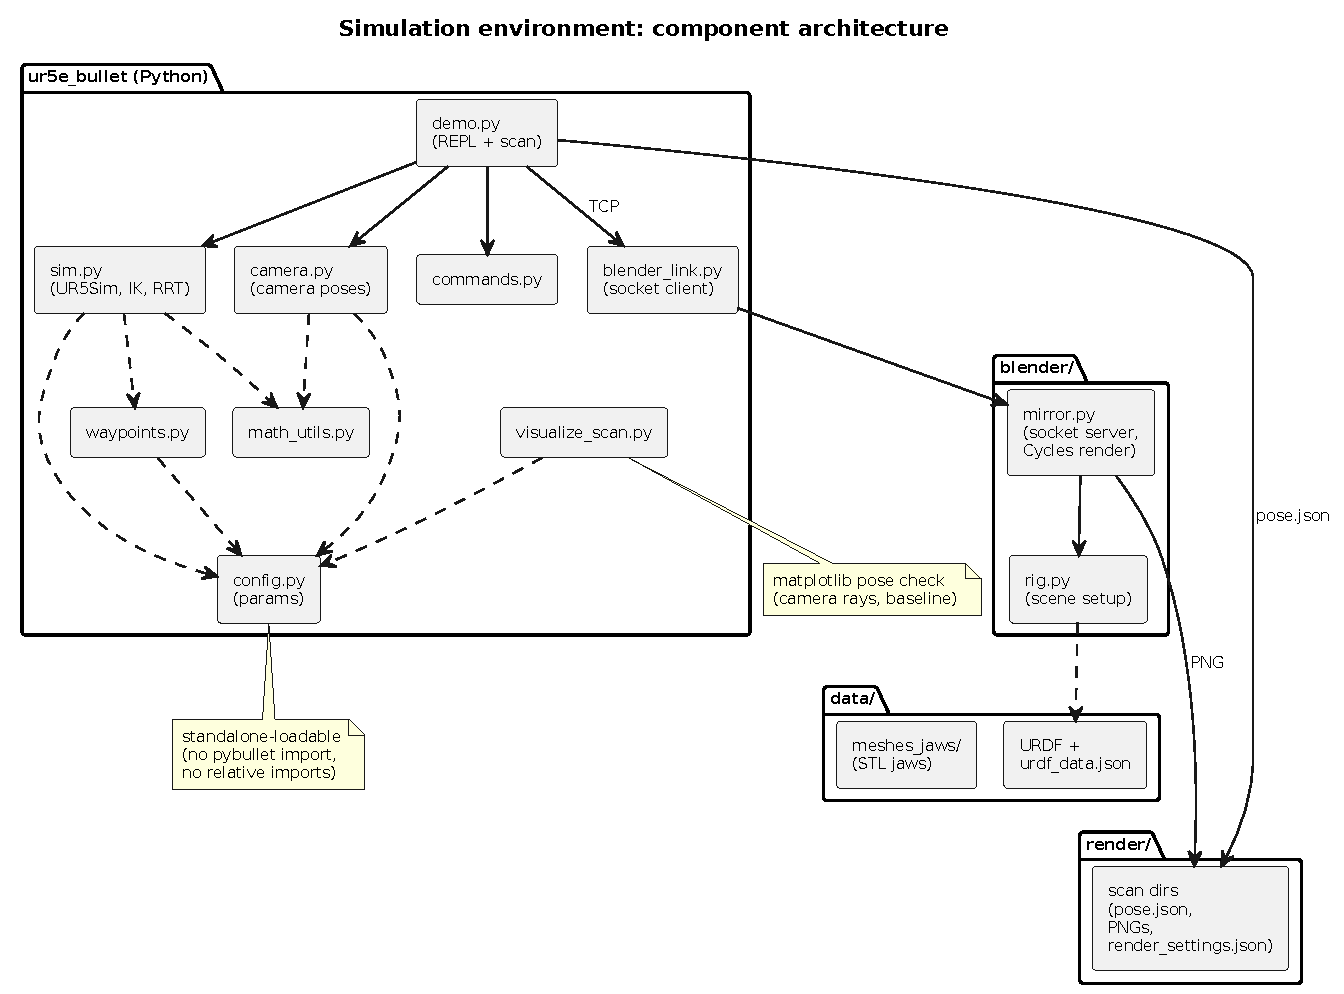
\includegraphics[width=\columnwidth]{assets/manuel/Architecture.pdf}
    \caption{Component architecture of the simulation environment. \code{config.py} is shared between the PyBullet pipeline and the Blender side.}
    \label{fig:ms-architecture}
\end{figure}

\subsubsection{Scan workflow}\label{ms:scan-workflow}

Starting from a user-selected start position with its jaw model loaded (STL geometry placed both in PyBullet and Blender), the scan sweep visits every
waypoint in order. At each waypoint the robot moves to the tool pose, the left/right camera poses are computed in the jaw frame and written to
\code{<n>\_pose.json}, and a render request for the left and right image is sent to Blender. Blender renders both views via Cycles on the GPU and
reports completion before the sweep advances. Figure~\ref{fig:ms-scan-workflow} shows the workflow; Figure~\ref{fig:ms-dataflow} details the message
and data flow for one waypoint together with the offline visualization step.

\begin{figure}[H]
    \centering
    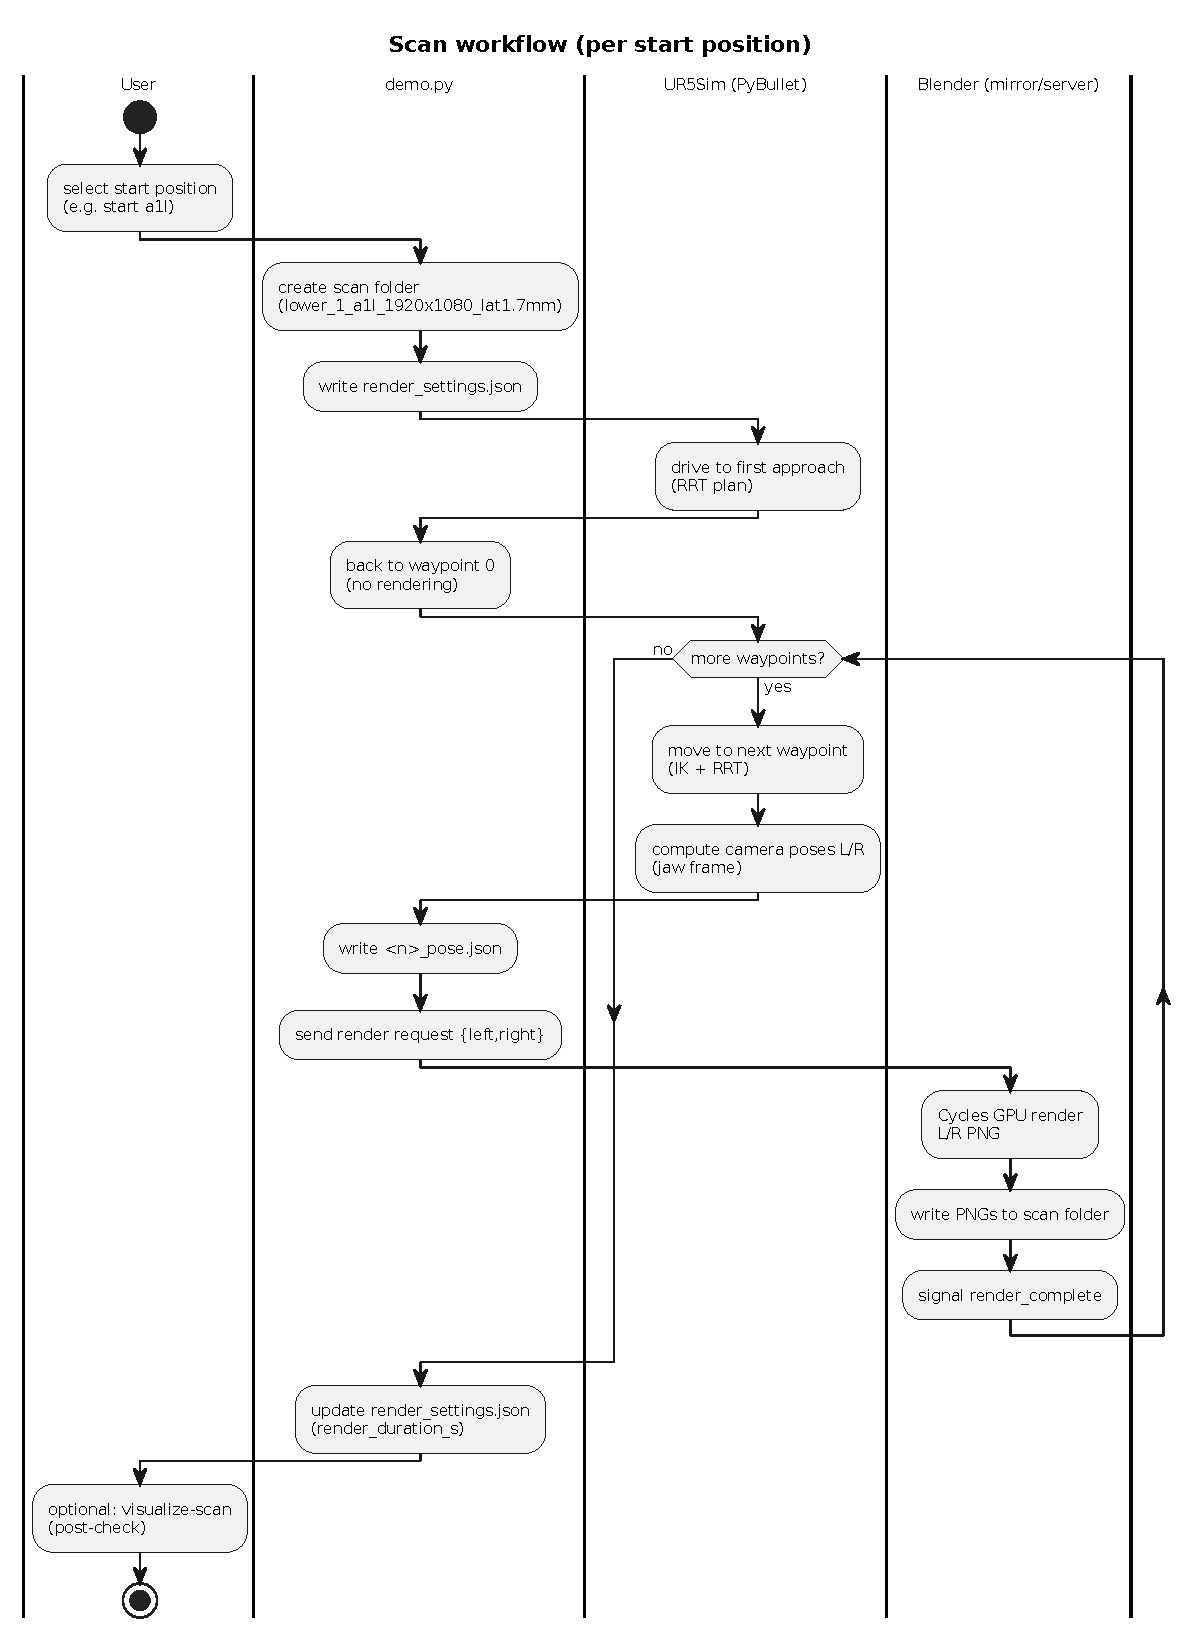
\includegraphics[width=\columnwidth]{assets/manuel/scan_workflow}
    \caption{Scan workflow for one start position. The sweep is driven by \code{demo.py}, executed by the PyBullet simulation and rendered by the Blender mirror.}
    \label{fig:ms-scan-workflow}
\end{figure}

\begin{figure}[H]
    \centering
    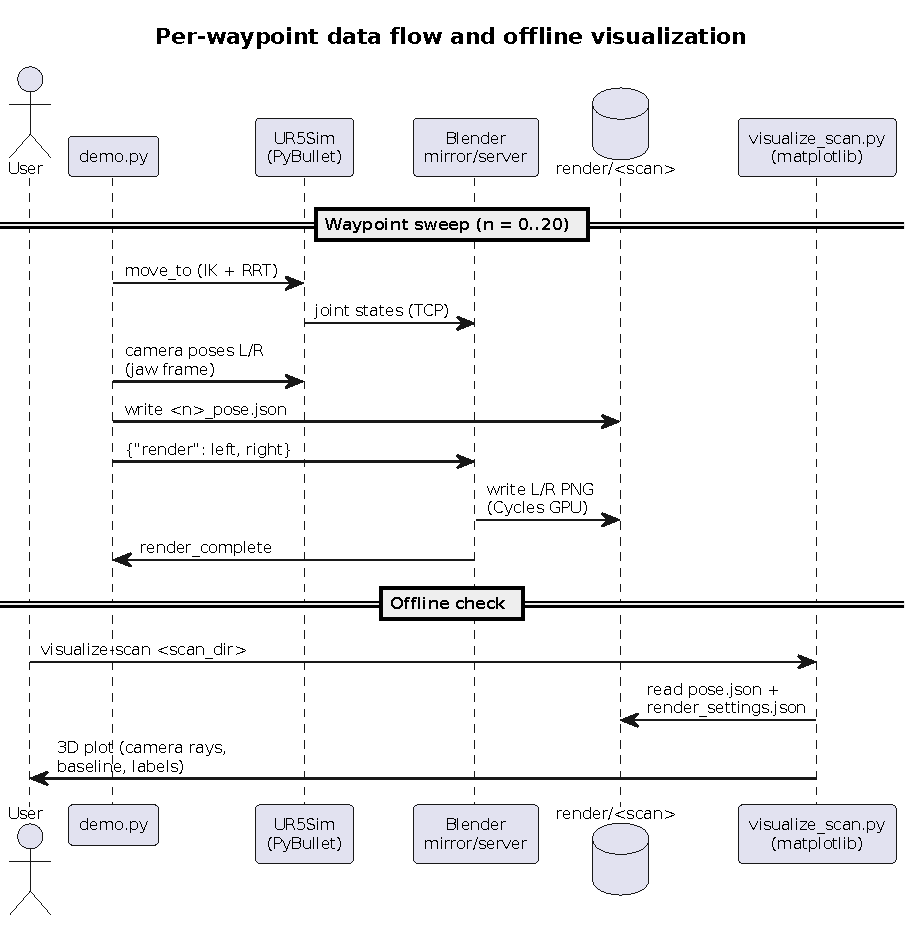
\includegraphics[width=\columnwidth]{assets/manuel/dataflow}
    \caption{Per-waypoint data flow and offline visualization of the exported camera poses.}
    \label{fig:ms-dataflow}
\end{figure}

\subsection{Usage}\label{ms:usage}

\subsubsection{Commands}\label{ms:commands}

The environment is started inside the project directory with the Poetry-managed dependencies:

\begin{itemize}[leftmargin=*]
    \item \code{poetry run ur5e} starts the PyBullet GUI, the Blender mirror and the interactive control loop.
    \item \code{start <name>} moves the arm to a start position and loads the jaw model (available: \code{a1l}, \code{a2l}, \code{aussen2}, \code{o1l}, \code{innen}).
    \item \code{scan [n]} drives all (or the first \code{n}) waypoints, saves the camera poses and renders the left/right images at each one.
    \item \code{scan-all <start1> [start2 ...]} runs \code{start} and a full \code{scan} for each given start position in sequence.
    \item \code{visualize-scan <scan\_dir|render/> [--out \ldots] [--ray-len m]} runs the offline pose check (Section~\ref{ms:visualization}).
\end{itemize}

\subsubsection{Configuration}\label{ms:config}

All parameters are collected in \code{src/ur5e\_bullet/config.py} and sorted by domain (paths, robot/kinematics, camera/sensor, rendering,
PyBullet GUI, visualization, jaw/material, Blender, scan positions). Central camera parameters used by both simulation and rendering are listed in
Table~\ref{tab:ms-camera-config}.

\begin{table}[H]
    \centering
    \small
    \caption{Central camera configuration parameters.}
    \begin{tabularx}{\columnwidth}{@{}>{\raggedright\arraybackslash}p{0.36\columnwidth} X@{}}
        \toprule
        \textbf{Parameter}                           & \textbf{Meaning}                                                                    \\
        \midrule
        \code{CAMERA_LATERAL_\newlineOFFSET}         & lateral offset of one camera from the scanner axis; \code{baseline\_m = 2 x offset} \\
        \code{CAMERA_FOV_DEG}, \code{CAMERA_LENS_MM} & horizontal field of view / lens focal length                                        \\
        \code{CAMERA_NEAR_M}, \code{CAMERA_FAR_M}    & near/far clipping planes of the pinhole camera                                      \\
        \code{CAMERA_ROLL_DEG}                       & roll of the camera rig around the viewing axis                                      \\
        \code{RENDER_W}, \code{RENDER_H}             & render resolution                                                                   \\
        \code{RENDER_ENGINE}, \code{RENDER_DEVICE}   & \code{CYCLES} on the \code{GPU}                                                     \\
        \code{START_POSITIONS}                       & start poses, approach poses and parabola waypoint generators                        \\
        \bottomrule
    \end{tabularx}
    \label{tab:ms-camera-config}
\end{table}

The \code{config.py} file is the only place to edit parameters; the values are forwarded into the live PyBullet session and, through the standalone
load, into Blender.

\subsubsection{Rendered dataset}\label{ms:results}

An example run with start position \code{a1l} produces the folder
\code{render/lower\_1\_a1l\_1920x1080\_lat1.7mm} containing 21 pose files
(\code{0\_pose.json} through \code{20\_pose.json}), 42 rendered PNGs (left/right per waypoint) and \code{render\_settings.json}. The pose file for each
waypoint stores \code{waypoint}, \code{label} and \code{camera\_left}/\code{camera\_right} with \code{position} and \code{quaternion} (x, y, z, w)
in the jaw coordinate frame. \code{render\_settings.json} stores the scan context (\code{start\_position}, jaw folder/type, jaw pose, render
resolution, engine/device, render duration) and the full reconstruction parameter block used by the stereo pipeline: \code{baseline\_m = 0.0034},
\code{camera\_fov\_deg = 87}, \code{camera\_lens\_mm $\approx$ 18.97}, \code{camera\_far\_m = 0.04}, \code{rectified = true},
\code{camera\_intrinsic} with \code{fx\_px = fy\_px = 1011.63}, \code{cx\_px = 960}, \code{cy\_px = 540} on a 36\,mm $\times$ 20.25\,mm sensor. A
second dataset with start position \code{o1l} is generated identically, which supports the stereo registration and model construction sections with
synthetic image pairs whose relative camera poses are known precisely.

\subsubsection{Visualization}\label{ms:visualization}

The offline pose visualization (\code{visualize-scan}) draws all camera rays (length = \code{camera\_far\_m}) from the \code{pose.json} files in the
jaw frame with \code{matplotlib}. As a \emph{positioning check} it shows the left (red) and right (blue) camera centers, the constant stereo baseline
(measured $\lvert \mathbf{L}-\mathbf{R}\rvert$, which should equal \code{baseline\_m}), the sweep order and the jaw bounding box. As an entry point
into the data work it provides the exact camera poses that feed the reconstruction pipeline, together with the ray geometry in orthographic
projection.

\subsubsection{Reconstruction reference}\label{ms:reconstruction}

The exported stereo pairs with known intrinsics and extrinsics are the input to the subsequent image acquisition and 3D reconstruction section. The
rectified left/right pairs enable standard stereo matching (e.g.\ SGM \cite{hirschmuller_stereo_2008} or learned methods such as IGEV-Stereo
\cite{xu_iterative_2023}) followed by point triangulation with the stated baseline; the \code{camera\_far\_m} value bounds the penetration of the
viewing rays into the jaw surface and can be used as a near-plane limit when triangulating intra-oral geometry. All pose files together realize the
photo-granular pose ground-truth that is otherwise hard to obtain for real intra-oral scans.
\chapterbreak

\section{title}
\sectionauthors{Sebastian Naglez}
\section{Sirona Omnicam Image Acquisition Investigation}

\subsection{Objective and Initial Approach}

The initial objective of this investigation was to obtain image data directly from the \textbf{Sirona Omnicam} for use within the DentaVision project. Access to the scanner's image stream was considered an important prerequisite for eventually integrating the scanner into the reconstruction pipeline and avoiding dependence on externally provided datasets or pre-existing scan data.

The initial approach was based on the assumption that the Omnicam could expose its camera or acquisition interface as a conventional USB device. Therefore, the first step was to investigate how the scanner was connected to the computer and whether its USB interface could provide a direct path to the acquired images. Both the \code{Windows Device Manager} and \code{USBTreeView} were used for this purpose. The connected devices and USB interfaces were inspected in an attempt to identify an entry corresponding to the Sirona Omnicam, or a device with a name or hardware information that could be associated with the scanner. USBTreeView was additionally used to inspect the available USB device information, interfaces, and endpoints in greater detail. This initial investigation did not provide a straightforward way to access the scanner's image data. In particular, identifying the device at the USB level did not imply that the image stream was exposed through a standard camera interface that could be accessed independently of the manufacturer's software. This led to a change in the investigation strategy.

Instead of treating the Omnicam as a conventional USB camera, the investigation was subsequently expanded to the \code{hardware, camera interfaces, drivers, acquisition SDK, and CEREC software stack}. The purpose was to determine how the scanner was actually exposed to the operating system and how the CEREC software interacted with the underlying hardware. This ultimately led to the investigation of the Matrix Vision camera components and, later, to reverse engineering of the software and DLLs used by \textbf{CEREC SW 5.1}.

\subsection{Camera and Acquisition Interface Investigation}

After the initial USB-level investigation, the focus shifted towards identifying the camera hardware used by the Omnicam and determining whether it could be accessed independently of the CEREC software. The investigation revealed that the scanner contained an industrial camera from MATRIX VISION, identified as a SiCamCCT camera belonging to the mvBlueCOUGAR family. The device was identified with serial number 27323555 and exposed a GenICam interface. The camera used an ICX424 sensor and communicated through GigE Vision.

The identification of the camera was significant because it provided a potential acquisition interface that could be investigated independently of the higher-level CEREC software. The Matrix Vision ecosystem includes tools and libraries for configuring and acquiring images from compatible devices. Therefore, the investigation focused on the mvIMPACT Acquire SDK and the associated wxPropView utility.

\subsubsection{Camera Detection and SDK Investigation}

The mvIMPACT Acquire SDK was used to investigate whether the camera could be detected and accessed directly. The device could be identified through the Matrix Vision acquisition software, confirming that the underlying camera hardware was accessible at this level. Several Matrix Vision components were also identified as being associated with the device, including libraries such as \code{mvDeviceManager.dll}, \code{mvBlueCOUGAR.dll} and \code{mvPropHandling.dll}. The wxPropView application was additionally used to inspect and configure the available camera properties. This provided access to acquisition-related parameters and helped determine whether the camera could be operated outside the normal CEREC acquisition workflow. The investigation also identified several image formats supported by the camera interface, including:

\begin{itemize}
    \item \code{RGB8Packed}
    \item \code{RGB20p12}
    \item \code{BGR8Packed}
    \item \code{BGR10V2Packed}
\end{itemize}

The availability of these formats indicated that the camera interface itself was capable of providing image data in standard color representations. However, this did not necessarily mean that the Omnicam used these formats during its normal scanning operation.

\subsubsection{Acquisition Attempts}

Despite successfully detecting the camera and accessing its configuration through the Matrix Vision tools, obtaining a usable image through direct acquisition initially proved unsuccessful. One of the main observed results was a black image being returned during acquisition attempts. This indicated that device detection and communication with the camera did not necessarily imply that the complete acquisition process used by the Omnicam had been correctly reproduced.

Acquisition parameters, particularly exposure-related settings, were investigated and adjusted in an attempt to determine whether the black image was caused by an incorrect configuration. A newer version of the mvIMPACT Acquire SDK was also installed and tested. After experimenting with different exposure settings and other available acquisition parameters, it was eventually possible to obtain an image in grayscale. However, this result did not provide a reliable acquisition path suitable for integration into an automated scanning pipeline. In addition, the mvIMPACT Acquire SDK did not provide a mechanism to control the scanner's projector, which was an important limitation because image acquisition alone would not be sufficient to reproduce the structured-light scanning process used by the Omnicam.

\subsubsection{Result and Limitations}

The investigation established that the Omnicam contained an identifiable Matrix Vision industrial camera that could be detected and accessed at the SDK level. The GenICam, GigE Vision, and mvIMPACT Acquire interfaces therefore provided a real hardware-level access point for further investigation. However, direct access to the camera through these interfaces was not sufficient to reproduce the scanner's normal image acquisition. Although a grayscale image could eventually be obtained, the acquisition process could not be demonstrated to provide the complete set of functionality required for automated scanning. In particular, the inability to control the scanner's projector through the available SDK represented a significant limitation. At this stage, the investigation therefore shifted from attempting to operate the camera solely through the Matrix Vision acquisition interface towards understanding how the CEREC software and its associated components controlled and interacted with the scanner.

\subsubsection{Investigation Method: Software Interaction and Reverse Engineering}

After the direct acquisition approach through the Matrix Vision interfaces failed to provide a complete and reliable way of obtaining the images required for the project, the investigation shifted towards understanding how the original CEREC software interacted with the scanner.

The main objective of this phase was to identify the software components responsible for communicating with and controlling the Omnicam and to determine whether the scanner's acquisition process could be reproduced or controlled outside the original CEREC environment. Particular attention was given to the possibility that the CEREC software performed additional operations that were not exposed through the standard Matrix Vision acquisition SDK.

The investigation began by examining the components used by CEREC SW 5.1 during scanner operation. Process Monitor was used to observe the activity of the software while interacting with the scanner. This provided information about the processes, dynamic-link libraries, files, and other system resources involved during the acquisition workflow. The collected information was used to identify potentially relevant components for further analysis. The identified binaries were subsequently investigated using Ghidra. The purpose of the reverse-engineering process was not to fully reconstruct the entire CEREC software, but to identify relevant functions, classes, data structures, and relationships that could provide information about the scanner's acquisition pipeline. Particular attention was given to the following DLLs:

\begin{itemize}
    \item \code{acquire.dll}
    \item \code{CAI2_CameraCCT.dll}
    \item \code{SiAcquireCtrl.dll}
    \item \code{mvPropHandling.dll}
    \item \code{MHT_ScannerLib.dll}
\end{itemize}

The analysis focused on finding evidence of functionality related to several stages of the scanning process. These included scanner initialization, starting and stopping the scanning process, image acquisition, and the transfer or processing of acquired data. In addition, the investigation specifically looked for code that could provide information about the structured-light system, particularly functions or components related to projector control, pattern generation or sequencing, and synchronization between the projected patterns and camera acquisition.

The latter aspects were particularly relevant because obtaining camera frames alone would not necessarily reproduce the Omnicam's scanning process. If the scanner relies on structured-light patterns, the acquired images would need to be synchronized with the corresponding projected patterns in order to reproduce the same type of measurement outside the original software. The reverse-engineering results were therefore used to construct a partial model of the scanner's software and data flow. Because this analysis was based primarily on decompiled binaries and indirect relationships between functions and components, the resulting architecture was treated as a set of working hypotheses rather than as a definitive description of the scanner's internal implementation. 

The analysis was also subject to significant practical limitations. The CEREC software consisted of numerous interconnected binaries and libraries, and not all components could be interpreted reliably or easily from their decompiled representation. Indirect calls, complex dependencies, compiler-generated structures, and the amount of available code made it difficult to follow the complete execution path. Consequently, the investigation was able to identify several relevant components and data flows, but it was not possible to reconstruct the complete scanner acquisition and reconstruction pipeline with certainty.

\subsection{Reverse Engineering Findings and Working Hypotheses}

The reverse-engineering analysis provided evidence of several components and data paths involved in the Omnicam's scanning process. However, the following reconstruction should not be understood as a definitive description of the scanner's internal architecture. It was derived primarily from decompiled binaries, identified class and function relationships, and the interpretation of data structures and buffers. Consequently, some elements are directly supported by the analyzed code, while others represent working hypotheses based on the observed relationships.

\subsubsection{Identified Components}

One of the main components identified during the analysis was \code{ScannerProxy}, which appears to provide a high-level abstraction of the scanner hardware. The analyzed code contains functions such as \code{ScannerProxy::StartScanning(bool enable)}, \longcode{ScannerProxy::CreateUsbScanData2D(...)}, and \longcode{ScannerProxy::CreateUsbScanData25D(...)}. The class also appears to provide access to a \code{MainFpgaProxy} object through a virtual function call. Based on the analyzed relationships, \code{ScannerProxy} was interpreted as a component connecting several parts of the acquisition process, including camera acquisition, FPGA-related processing, and the creation of scan-data objects. \code{MainFpgaProxy} appears to represent an interface to the scanner's internal FPGA. Among the identified functions are \longcode{IsInterpolatedPeaksUsbData()}, \longcode{motor\_hard\_stop\_front\_in\_micrometers()}, and \longcode{motor\_hard\_stop\_back\_in\_micrometers()}. The presence of these functions suggests that the FPGA interface is associated not only with data processing but also with aspects of the scanner's mechanical control.

The analysis also identified a hierarchy of scan-data objects. \code{ScanData} appears to act as a high-level container holding references to two different types of data, which were interpreted as \code{ScanData2D} and \code{ScanData25D}. The constructors observed in the decompiled code copy two independent \code{shared_ptr} objects, which is consistent with such a structure, although the complete original class definition could not be recovered. \code{ScanData2D} appears to represent the two-dimensional camera data. The function \code{ScanDataHelper::GetRawTwoDScanData()} was identified together with parameters corresponding to image width, height, and a raw data buffer. The analysis also identified. \longcode{TwoDCameraProcess::DebayerBayeredImage()}, providing evidence for a Bayer image processing stage. \code{ScanData25D}, in contrast, appears to represent processed data associated with the scanner's three-dimensional acquisition. The analyzed code distinguishes between raw and interpolated peak data. Depending on the selected mode, the data appears to be encapsulated in either \code{UsbScanData25D} or \code{UsbScanData25DInterpolatedPeaks}. Several constructors associated with these objects were also identified:

\begin{itemize}
    \item \code{FUN_180177750} $\rightarrow$ \code{UsbScanData25D}
    \item \code{FUN_180177850} $\rightarrow$ \longcode{UsbScanData25DInterpolatedPeaks}
    \item \code{FUN_180177960} $\rightarrow$ \code{UsbScanData2D}
    \item \code{FUN_180183310} $\rightarrow$ \code{UsbScanData2D}
\end{itemize}

These functions were interpreted as object constructors rather than as functions performing the actual three-dimensional reconstruction.

\subsubsection{Identified Data Paths}

The analysis provided stronger evidence for the two-dimensional camera-data path than for the complete three-dimensional reconstruction pipeline. The identified camera configuration and the observed \longcode{TwoDCameraProcess::DebayerBayeredImage()} call suggest that the scanner can acquire image data in a Bayer mosaic representation before converting it to RGB through software processing. The corresponding data path can therefore be represented as:

\[
\text{Camera}
\rightarrow
\text{RAW Bayer}
\rightarrow
\text{Debayer}
\rightarrow
\text{RGB}
\]

This interpretation is supported by the identification of the Bayer acquisition mode and the explicit debayering function in the analyzed code. 

The creation of \code{ScanData2D} also provided evidence of a raw byte buffer being passed into the scanner's data structures. In particular, \longcode{ScannerProxyQcc61::CreateUsbScanData2D(...)} accepts a \code{shared_ptr<vector<unsigned char>>} together with image dimensions. During the construction process, an ROI object was also observed, suggesting that the useful image region may be defined at this stage. The exact role and contents of all associated metadata, however, could not be established with certainty.

A separate data path appears to originate from the FPGA. The analyzed code distinguishes between raw peaks and interpolated peaks, controlled by the result of \longcode{MainFpgaProxy::IsInterpolatedPeaksUsbData()}. The corresponding conceptual flow was interpreted as:

\[
\resizebox{\columnwidth}{!}{$
\text{FPGA}
\rightarrow
\text{Raw or Interpolated Peak Data}
\rightarrow
\text{ScanData25D}
$}
\]

The observed object sizes were approximately 12,776 bytes (\code{0x31E8}) for the normal representation and 10,760 bytes (\code{0x2A08}) for the interpolated representation. These values provide evidence that different internal data representations are used, although their complete binary structure was not determined.

Overall, the analyzed code suggests that the scanner handles at least two related data streams: a two-dimensional camera stream and a second stream containing peak or height-related information. These streams are subsequently represented through the \code{ScanData2D} and \code{ScanData25D} structures.

\subsubsection{Partial Reconstruction of the Acquisition Flow}

Based on the identified functions and relationships, a partial reconstruction of the acquisition flow was developed. When the user initiates a scan, \code{ScannerProxy::StartScanning(bool enable)} appears to initiate or enable the scanning process. During this process, the \code{ScannerProxy} is associated with both camera-related functionality and the \code{MainFpgaProxy}. The analyzed relationships suggest the following conceptual flow:

\[
\resizebox{\columnwidth}{!}{$
\text{Scan Initiation}
\rightarrow
\text{ScannerProxy::StartScanning()}
\rightarrow
\begin{cases}
\text{Camera Acquisition}\\
\text{FPGA-related Processing}
\end{cases}
$}
\]

The camera-related path appears to produce RAW Bayer data that is subsequently processed through software debayering and represented as \code{ScanData2D}. In parallel, the FPGA-related path appears to produce peak or height-related data that is represented as \code{ScanData25D}. This can be summarized as:

\[
\resizebox{\columnwidth}{!}{$
\begin{array}{ccc}
& \text{ScannerProxy} & \\
& \swarrow \qquad \searrow & \\\\
\text{Camera} && \text{Main FPGA} \\
\downarrow && \downarrow \\
\text{RAW Bayer} && \text{Peak/Height Data} \\
\downarrow && \downarrow \\
\text{ScanData2D} && \text{ScanData25D} \\
\downarrow && \downarrow \\
\text{Debayer / RGB} && \text{Processed 2.5D Data}
\end{array}
$}
\]

This represents a working model rather than a fully verified implementation. In particular, the analysis did not establish that \code{StartScanning()} itself directly controls every stage of the acquisition process. Instead, it appears to initiate a larger sequence in which other modules perform the camera, FPGA, and potentially optical operations. The presence of the message ``Generating faked volume data!'' during the analysis of \code{StartScanning()} also suggests that the software contains an internal simulation or testing mode capable of generating artificial volume data. This provides additional evidence that the scanner software contains different internal acquisition and processing paths, although the exact purpose and activation conditions of this mode could not be fully established.

\subsubsection{Inferred Working Model of the Acquisition and Data Flow}

Based on the available evidence, the following model represents the most plausible interpretation of the scanner's acquisition architecture at the time of the investigation:

\begin{figure}[H]
    \centering
    \resizebox{\columnwidth}{!}{%
    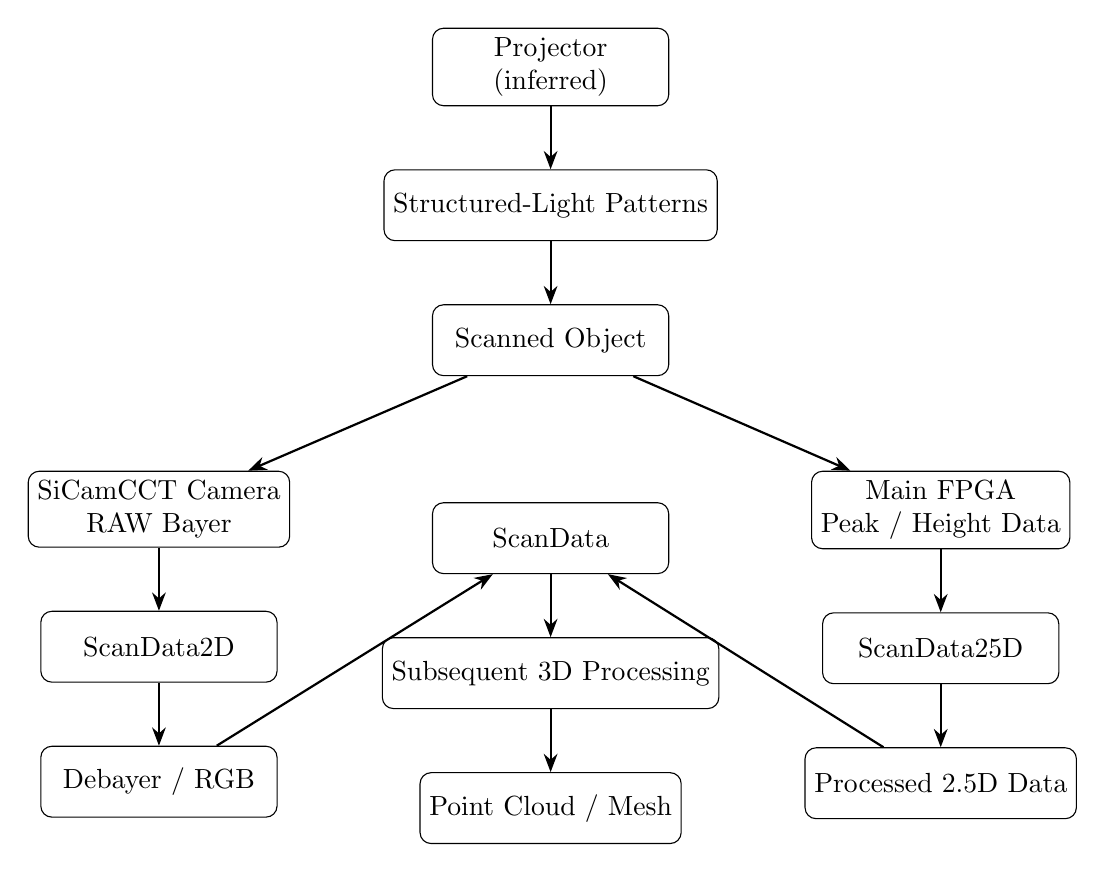
\begin{tikzpicture}[
        node distance=8mm and 18mm,
        box/.style={
            draw,
            rounded corners,
            align=center,
            minimum width=30mm,
            minimum height=9mm
        },
        arrow/.style={
            -{Stealth},
            thick
        }
    ]

        % Top
        \node[box] (projector) {Projector\\(inferred)};

        \node[box, below=of projector] (patterns)
            {Structured-Light Patterns};

        \node[box, below=of patterns] (object)
            {Scanned Object};

        % Camera and FPGA branches
        \node[box, below left=12mm and 18mm of object] (camera)
            {SiCamCCT Camera\\RAW Bayer};

        \node[box, below right=12mm and 18mm of object] (fpga)
            {Main FPGA\\Peak / Height Data};

        \node[box, below=of camera] (scan2d)
            {ScanData2D};

        \node[box, below=of fpga] (scan25d)
            {ScanData25D};

        \node[box, below=of scan2d] (debayer)
            {Debayer / RGB};

        \node[box, below=of scan25d] (processed)
            {Processed 2.5D Data};

        % Merge
        \node[box, below=16mm of object] (scandata)
            {ScanData};

        \node[box, below=of scandata] (processing)
            {Subsequent 3D Processing};

        \node[box, below=of processing] (output)
            {Point Cloud / Mesh};

        % Arrows
        \draw[arrow] (projector) -- (patterns);
        \draw[arrow] (patterns) -- (object);

        \draw[arrow] (object) -- (camera);
        \draw[arrow] (object) -- (fpga);

        \draw[arrow] (camera) -- (scan2d);
        \draw[arrow] (fpga) -- (scan25d);

        \draw[arrow] (scan2d) -- (debayer);
        \draw[arrow] (scan25d) -- (processed);

        % Merge into ScanData
        \draw[arrow] (debayer) -- (scandata);
        \draw[arrow] (processed) -- (scandata);

        \draw[arrow] (scandata) -- (processing);
        \draw[arrow] (processing) -- (output);

    \end{tikzpicture}%
    }
    \caption{Inferred data flow of the Omnicam scanning pipeline.}
    \label{fig:omnicam-data-flow}
\end{figure}

The camera, FPGA, \code{ScanData2D}, and \code{ScanData25D} relationships shown in this model are supported to varying degrees by the analyzed code. The projector, structured-light pattern generation, synchronization, and final three-dimensional processing are included as inferred components rather than confirmed findings.

\subsubsection{Unresolved Components and Limitations}

Despite identifying several important components, significant parts of the acquisition pipeline remained unresolved. The most important unresolved component was the projector control. The analysis did not identify explicit functions or modules clearly associated with terms such as \code{Projector}, \code{Pattern}, \code{GrayCode}, \code{PhaseShift}, \code{DLP}, \code{Sequence}, \code{Projection}, \code{LED}, or \code{Laser}. Consequently, no direct evidence was found showing where the structured-light patterns were generated or how the projector was controlled. Similarly, the synchronization mechanism between the projector and camera could not be identified. A complete automated acquisition process would likely require coordination between the projected pattern and the corresponding camera exposure, but the specific mechanism responsible for this synchronization remained unknown. The exact format of the internal data buffers was another unresolved aspect. Although several buffers were identified as \code{vector<unsigned char>} objects and their approximate sizes could be determined, their internal fields could not be fully reconstructed. Elements such as headers, frame identifiers, timestamps, peak values, calibration information, or coordinates could therefore not be confirmed. The final processing stages were also not fully identified. Although the presence of \code{ScanData25D} suggests that data related to three-dimensional acquisition is generated before later processing, the exact component responsible for transforming this information into a point cloud, mesh, or final three-dimensional model was not established.

Finally, the reverse-engineering process itself imposed substantial limitations. The CEREC software consisted of numerous interconnected DLLs, and several binaries were difficult to interpret reliably using decompilation. Indirect calls, compiler-generated structures, dependencies between modules, and the complexity of the assembly code made it difficult to trace complete execution paths. As a result, the analysis was sufficient to identify several relevant components and construct a plausible working model, but not to verify the complete internal architecture of the Omnicam with certainty or to identify a self-contained function that could be invoked from custom software to initiate and reproduce the complete scanning process.


\subsection{UDP Communication and Data Capture Investigation}

\subsubsection{Initial UDP Communication and API Prototype}

During the investigation of the scanner control commands, a small prototype API was developed in parallel to explore how a programmable scanner interface could be structured if a suitable command for initiating the scan could be identified. At this stage, it was still assumed that such a command might be available and that it could potentially be integrated into a custom acquisition interface. The intended concept was to provide an interface capable of connecting to the scanner, initiating a scan through a command identified during the reverse-engineering process, receiving the resulting data, and subsequently forwarding it to the DentaVision processing pipeline. The objective was therefore not to provide a complete scanner implementation, but to investigate the software structure that could be used for such an interface. The prototype introduced an abstract hardware interface with operations for connecting to the scanner, projecting a pattern, capturing an image, and disconnecting from the device. A mock implementation was used to simulate these operations and to verify the intended control flow. A higher-level \code{Scanner} class could then execute a sequence consisting of connecting to the hardware, projecting several patterns, capturing the corresponding images, and disconnecting. This prototype was developed as a preliminary representation of the intended scanner-control architecture rather than as a functional interface to the physical Omnicam. Once the investigation progressed and no suitable command for independently initiating the scanning process could be identified, the prototype was no longer pursued as a means of controlling the physical scanner.

\subsubsection{Investigation and Reproduction of GVCP Commands}

As the reverse-engineering analysis had not identified a directly usable function for starting the scan from custom software, the network communication between the scanner and the CEREC software was investigated. The motivation for this approach came from observing the network activity of the system during a scan. In the Windows Task Manager, Ethernet usage increased noticeably when a scan was initiated in the CEREC software, suggesting that a significant amount of data could be exchanged through the network interface. This raised the possibility that the scanner might communicate with the CEREC software over the network, leading to the use of Wireshark to capture and investigate the corresponding traffic. Wireshark was used to observe the UDP traffic generated during scanner operation. Particular attention was given to communications occurring before and around the beginning of a scan, with the objective of identifying commands that could potentially be reproduced independently of the original software.

Based on this investigation, a C++ implementation of a UDP communication layer was developed. The \code{UDPClient} class provided basic UDP packet transmission and reception, while \code{GvcpClient} implemented read and write operations for registers using the observed GVCP command structure. A \code{GvcpSequence} class was additionally implemented to execute a series of register operations in a defined order.
Several register addresses were investigated and sequences containing read and write operations were tested. The scanner responded to some of the transmitted commands, demonstrating that communication with the device could be established through the implemented UDP interface. However, reproducing the complete sequence required to initiate the scanning process was not achieved. Consequently, although the experiment demonstrated that the scanner could respond to custom UDP/GVCP communication, it did not provide a reliable method for starting an acquisition independently from the CEREC software.

\subsubsection{Direct Capture of Scanner Data}

After the attempt to initiate the scanning process through reproduced commands was unsuccessful, a different approach was investigated. Instead of attempting to control the scanner directly, the CEREC software was used to initiate the scan manually while the custom program listened for the data transmitted by the scanner. A UDP receiver was implemented in C++ specifically for this purpose. The \code{GvspReceiver} class opened a UDP socket on the investigated GVSP port and waited for incoming datagrams. The received packets were inspected to extract information interpreted as block identifiers, packet identifiers, and packet types. The receiver attempted to distinguish between leader, data, and trailer packets and to group packets belonging to the same block. Data packets were then processed by removing the interpreted packet header and appending the remaining bytes to an output buffer. The accumulated data were subsequently written to a binary file named \code{frame.raw}. In addition, a separate \code{GvspAnalyzer} component was implemented to inspect previously captured data. It divided the captured stream into fixed-size packets and reported the interpreted block and packet identifiers, allowing the structure and continuity of the received data to be investigated. This implementation therefore demonstrated that data transmitted by the scanner could be captured independently of the CEREC application's normal display path and stored for further analysis.

\subsubsection{Observed Behaviour During Data Capture}

An important observation was made while performing the direct data-capture experiment. When the custom receiver was connected to the investigated communication port and started receiving the scanner's transmitted data, the live image that normally appeared in the CEREC software stopped being displayed. This behaviour was considered potentially significant because it suggested that the captured traffic could be related to the data stream used by the scanner during acquisition. However, the observation alone was not sufficient to establish that the received packets represented the camera images directly.

In particular, the internal architecture analysis had already indicated that the scanner may exchange multiple types of data associated with the acquisition and 3D reconstruction process. Therefore, the captured stream could potentially contain image data, processed 3D-related data, metadata, or a combination of different data types. The possibility of additional encoding or an undocumented internal data format also could not be excluded. Consequently, the disappearance of the live image was treated as an indication that the captured traffic was relevant to the scanner's acquisition process, rather than as definitive evidence that the received bytes constituted directly usable image frames.

\subsubsection{Data Interpretation and Limitations}

Although the C++ receiver successfully captured and stored data transmitted by the scanner, the complete structure and meaning of the received stream could not be established. The captured binary data could not be reliably reconstructed into usable image frames. The investigation therefore did not establish whether the received data consisted exclusively of camera images, contained a combination of image and 3D-related information, or used an additional encoding or proprietary representation. The packet-level analysis provided information about the apparent structure of the communication, but it was insufficient to reconstruct the complete payload semantics.
As a result, the \code{frame.raw} output should be understood as a capture of received binary data rather than as a successfully reconstructed image.

Combined with the lack of a reliable method for initiating the scan programmatically, the limited available documentation, and the difficulty of determining the internal data representation, this approach was ultimately considered impractical for obtaining image data from the Omnicam for the DentaVision pipeline. The scanner was therefore not used as the image source for the subsequent development. Instead, image acquisition was moved to the project's virtual/simulated pipeline, where the required camera input could be provided while allowing the remaining DentaVision processing and reconstruction pipeline to be developed independently of the limitations encountered with the physical scanner.

\subsection{Conclusion and Future Considerations}

The investigation successfully identified the main camera hardware and acquisition interfaces, provided access to relevant device information, examined the available SDKs, identified several relevant software components, and allowed parts of the scanner's acquisition and data flow to be inferred through reverse engineering. It was also possible to establish UDP communication with the scanner and capture data transmitted during an acquisition. However, no reliable method was found to obtain directly usable images for the DentaVision pipeline, fully control the scanner, identify the synchronization mechanism of the structured-light system, or completely interpret the captured data.

As a result, the investigation of direct image acquisition from the Omnicam was concluded, and the scanner was not used as the image source for the subsequent development of DentaVision. Nevertheless, the work provided a partial understanding of the scanner's internal architecture and identified several relevant acquisition and processing paths. For future investigations, the use of a programmable scanner with documented access to its acquisition process would be preferable.


% 3d reconstruction
\section{3D Reconstruction}

\subsection{Theoretical Background}

Three-dimensional reconstruction from images can be approached through different computer vision paradigms. The methods investigated in this project range from feature-based reconstruction and Structure-from-Motion (SfM) to classical stereo matching and learning-based stereo estimation. Although these approaches differ in their assumptions and internal processing, they all rely on establishing relationships between different observations of the same scene in order to infer three-dimensional information.

The following sections introduce the main concepts required to understand the reconstruction methods implemented and evaluated in this work. The discussion begins with feature-based correspondence using the Scale-Invariant Feature Transform (SIFT), followed by Structure-from-Motion, classical stereo vision and disparity estimation, and finally learning-based stereo matching using IGEV-Stereo.

\subsubsection{Feature-Based Reconstruction and SIFT}

Feature-based reconstruction relies on identifying distinctive visual structures in one or more images and establishing correspondences between observations of the same physical points. These correspondences provide the basis for estimating geometric relationships between images and, ultimately, recovering three-dimensional information about the observed scene.

A typical feature-based pipeline consists of two main stages: feature detection and feature description. First, visually distinctive locations, commonly referred to as \textit{keypoints}, are identified within each image. A descriptor is then computed for the local image region surrounding each keypoint. The descriptors can subsequently be compared between images to determine which keypoints are likely to represent the same physical location. One of the most widely used feature extraction methods is the Scale-Invariant Feature Transform (SIFT), introduced by Lowe \cite{lowe_distinctive_2004}. SIFT detects distinctive image features across different scales and computes a descriptor that characterizes the local appearance around each detected keypoint. An important property of the method is its invariance to image scale and rotation, while also providing robustness to moderate changes in viewpoint, illumination, noise and affine distortion \cite{lowe_distinctive_2004}.

After features have been extracted from multiple images, their descriptors can be compared to establish candidate correspondences. These correspondences are subsequently filtered using geometric constraints in order to remove incorrect matches. The resulting set of reliable correspondences can then be used by higher-level reconstruction algorithms to estimate camera motion or recover the three-dimensional position of observed points. In the context of three-dimensional reconstruction, SIFT therefore does not directly generate a three-dimensional model. Instead, it provides the feature correspondences required by subsequent geometric operations such as pose estimation and triangulation. This distinction is particularly relevant to the reconstruction approaches investigated in this project, where SIFT was used as the basis for both pairwise reconstruction and Structure-from-Motion pipelines.

An inherent limitation of feature-based reconstruction is its dependence on the availability of sufficiently distinctive visual features. Regions with little texture, homogeneous appearance or repetitive structures may provide fewer reliable keypoints and correspondences. As a result, the performance of feature-based approaches can vary considerably depending on the visual characteristics of the observed scene. This limitation motivated the subsequent evaluation of alternative reconstruction approaches based on stereo disparity estimation.

\subsubsection{Structure-from-Motion}

Structure-from-Motion is a computer vision approach that estimates the three-dimensional structure of a scene together with the relative positions and orientations of the cameras from multiple images. Starting from correspondences between image features, SfM jointly recovers the geometry of the observed scene and the motion or pose of the cameras that captured it \cite{szeliski_computer_2022,schonberger_structure--motion_2016}.
A simplified SfM pipeline can be described as follows:

\begin{center}
\resizebox{\columnwidth}{!}{%
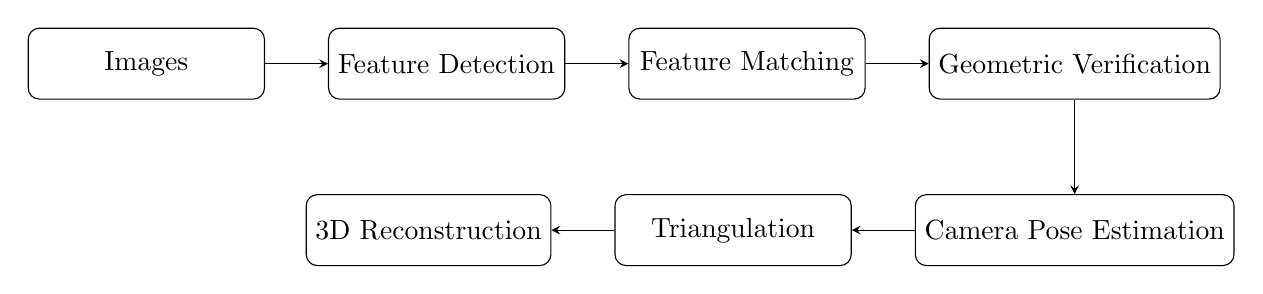
\begin{tikzpicture}[
    box/.style={
        rectangle,
        draw,
        rounded corners,
        align=center,
        minimum width=3.0cm,
        minimum height=0.9cm
    },
    arrow/.style={
        ->,
        >=stealth
    }
]

\node[box] (images) {Images};
\node[box, right=0.8cm of images] (detection) {Feature Detection};
\node[box, right=0.8cm of detection] (matching) {Feature Matching};
\node[box, right=0.8cm of matching] (verification) {Geometric Verification};

\node[box, below=1.2cm of verification] (pose) {Camera Pose Estimation};
\node[box, left=0.8cm of pose] (triangulation) {Triangulation};
\node[box, left=0.8cm of triangulation] (reconstruction) {3D Reconstruction};

\draw[arrow] (images) -- (detection);
\draw[arrow] (detection) -- (matching);
\draw[arrow] (matching) -- (verification);

\draw[arrow] (verification) -- (pose);
\draw[arrow] (pose) -- (triangulation);
\draw[arrow] (triangulation) -- (reconstruction);

\end{tikzpicture}%
}
\end{center}

The process begins by detecting and matching features between images. The resulting correspondences are used to estimate the geometric relationship between different camera views. In the case of calibrated cameras, this relationship can be represented through the essential matrix, which encodes the relative rotation and translation between two camera views. Once the relative camera poses have been estimated, corresponding image observations can be triangulated to estimate the three-dimensional position of the observed points. The reconstructed three-dimensional points are commonly referred to as \textit{landmarks}. In multi-view reconstruction, the same landmark may be observed in several images. Maintaining the association between these individual observations and their corresponding three-dimensional points requires the management of \textit{tracks}, which represent groups of feature observations that are assumed to correspond to the same physical point. As additional images are incorporated into the reconstruction, the estimated camera poses and three-dimensional landmarks are refined through bundle adjustment. Bundle adjustment jointly optimizes the reconstruction parameters in order to minimize the reprojection error between the observed image features and the projections of the estimated three-dimensional points \cite{szeliski_computer_2022}.

Although the individual operations involved in SfM can be implemented using general-purpose computer vision libraries, constructing a complete and robust SfM pipeline requires managing feature correspondences, tracks, camera poses, landmarks and iterative optimization. Modern SfM systems therefore integrate these operations into specialized reconstruction pipelines. For example, Schönberger and Frahm describe an incremental Structure-from-Motion pipeline designed to improve robustness, accuracy, completeness and scalability when reconstructing scenes from unordered image collections \cite{schonberger_structure--motion_2016}. This complexity was directly relevant to the development of the reconstruction pipeline in this project. An initial manual implementation demonstrated that performing individual operations such as feature matching, pose estimation and triangulation was not sufficient to construct a complete multi-view reconstruction system without additionally managing the relationships and consistency between all observations. Consequently, established SfM and multi-view reconstruction tools were later investigated as an alternative to implementing the complete pipeline manually.

\subsubsection{Stereo Vision and Disparity}

Stereo vision estimates three-dimensional information by observing the same scene from two different viewpoints. In a stereo camera configuration, two cameras observe the scene from slightly different positions. Consequently, the projection of the same physical point appears at different image locations in the left and right images. After the stereo images have been rectified, corresponding points are typically located along the same horizontal image coordinate. This simplifies the correspondence problem by reducing the search for matching points primarily to the horizontal direction. The horizontal displacement between corresponding points is referred to as \textit{disparity}.
For a rectified stereo pair, disparity can be expressed as

\begin{equation}
d = x_L - x_R
\label{eq:disparity}
\end{equation}

where \(x_L\) and \(x_R\) represent the horizontal coordinates of corresponding points in the left and right images, respectively. The estimated disparity is inversely related to the depth of the observed point. For an ideal stereo configuration, depth can be calculated as

\begin{equation}
Z = \frac{fB}{d}
\label{eq:depth_from_disparity}
\end{equation}

where \(Z\) represents the depth, \(f\) is the focal length, \(B\) is the baseline between the two camera centers, and \(d\) is the disparity. Therefore, points with a larger disparity are generally located closer to the cameras, whereas points with a smaller disparity are located farther away \cite{opencv_depth_map_stereo, opencv_camera_calibration}.

The main challenge in stereo reconstruction is the correspondence problem: determining which pixel or image region in the left image corresponds to the same physical point in the right image. Stereo matching algorithms estimate these correspondences and generate a \textit{disparity map}, in which each valid pixel is associated with an estimated horizontal displacement. Classical stereo matching methods generally combine a matching cost with spatial regularization. The matching cost evaluates the similarity between candidate image regions, while the regularization process encourages geometrically consistent disparity estimates across neighboring pixels. One influential approach is Semi-Global Matching (SGM), proposed by Hirschmüller \cite{hirschmuller_stereo_2008}. SGM approximates global energy optimization by aggregating matching costs along multiple paths through the image while incorporating smoothness constraints. This allows the method to balance local image similarity with spatial consistency without performing a computationally expensive global optimization.

The Stereo Semi-Global Block Matching implementation provided by OpenCV, referred to as StereoSGBM, follows this general class of stereo matching approaches and was used in this project to generate disparity maps from rectified stereo image pairs. The resulting disparity estimates were subsequently used to reconstruct depth and three-dimensional point clouds. Unlike Structure-from-Motion, which estimates camera motion and scene structure from multiple observations, stereo reconstruction can directly estimate depth from the disparity between two views when the relevant camera parameters and stereo geometry are known. This makes stereo matching particularly suitable for evaluating the reconstruction of individual image pairs.

\subsubsection{Learning-Based Stereo Matching and IGEV}

Classical stereo matching methods rely on explicitly designed similarity measures and optimization strategies to establish correspondences between stereo images. Their performance can be affected by ambiguous correspondences, low-texture regions, repetitive patterns and other image characteristics that make it difficult to identify corresponding pixels reliably. Learning-based stereo matching approaches address the correspondence problem by using neural networks trained on stereo data. Instead of relying exclusively on manually designed image features or matching costs, these methods learn feature representations and correspondence relationships from training data. During inference, a trained model receives a stereo image pair and estimates a disparity map representing the relative displacement between corresponding pixels.

One such method is IGEV-Stereo, proposed by Xu et al. \cite{xu_iterative_2023}. IGEV-Stereo introduces the Iterative Geometry Encoding Volume, a representation designed to combine geometric and contextual information with local matching information. The resulting representation is used iteratively to refine the estimated disparity map. The method builds upon iterative stereo estimation approaches but introduces additional geometric information into the representation used during disparity refinement. According to Xu et al., the geometry encoding volume is designed to provide information that is not sufficiently represented by conventional all-pairs correlation alone, particularly in ambiguous or ill-posed image regions \cite{xu_iterative_2023}.

An important distinction between the learning-based approach used in this project and the development of a neural network from scratch is the use of a pretrained model. Training a stereo network requires a substantial amount of stereo data, computational resources and optimization time. Instead, the implementation evaluated in this work used a pretrained IGEV model to perform inference on the selected stereo image pairs.
The reconstruction process can therefore be summarized as

\begin{center}
\resizebox{\columnwidth}{!}{%
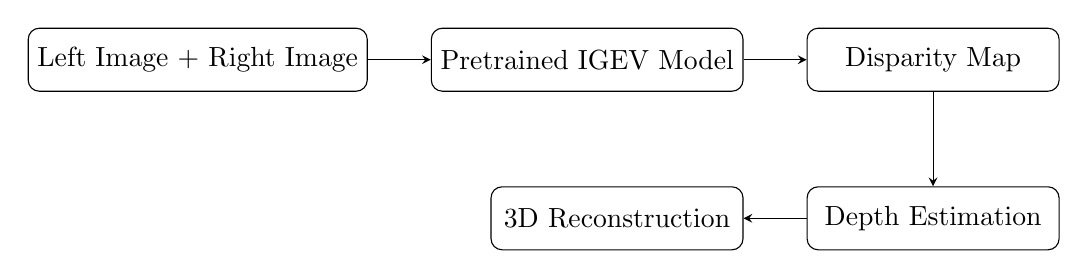
\begin{tikzpicture}[
    box/.style={
        rectangle,
        draw,
        rounded corners,
        align=center,
        minimum width=3.2cm,
        minimum height=0.8cm
    },
    arrow/.style={
        ->,
        >=stealth
    }
]

% First row
\node[box] (input) {Left Image + Right Image};
\node[box, right=0.8cm of input] (model) {Pretrained IGEV Model};
\node[box, right=0.8cm of model] (disparity) {Disparity Map};

% Second row
\node[box, below=1.2cm of disparity] (depth) {Depth Estimation};
\node[box, left=0.8cm of depth] (reconstruction) {3D Reconstruction};

% Arrows
\draw[arrow] (input) -- (model);
\draw[arrow] (model) -- (disparity);
\draw[arrow] (disparity) -- (depth);
\draw[arrow] (depth) -- (reconstruction);

\end{tikzpicture}%
}
\end{center}

This approach allowed the learning-based stereo method to be integrated into the reconstruction pipeline without performing model training. The resulting disparity maps could then be evaluated using the same underlying stereo geometry used for the classical StereoSGBM approach. 

Together, feature-based reconstruction, Structure-from-Motion, classical stereo matching and learning-based stereo estimation represent different approaches to recovering three-dimensional information from images. The following sections describe how these approaches were implemented and evaluated within the project, beginning with feature-based pairwise reconstruction using SIFT.

\subsection{Pairwise Feature-Based Reconstruction with SIFT}

One of the reconstruction approaches investigated in the project is a
feature-based pairwise reconstruction pipeline using the
\textbf{Scale-Invariant Feature Transform (SIFT)}. The purpose of this
approach was to investigate whether sparse 3D geometry could be reconstructed
directly from corresponding features between individual image pairs. This approach represents only one of the reconstruction strategies explored
in the project. It was selected as a relatively simple implementation of
two-view Structure from Motion (SfM), allowing the individual geometric
components of the reconstruction process to be investigated independently.
The resulting sparse point clouds were also suitable for subsequent
processing, such as point cloud registration. Unlike a complete multi-view SfM system, the implementation does not attempt
to maintain a globally consistent reconstruction across an entire image
sequence. Instead, each image pair is processed independently. This
substantially reduces the complexity of the reconstruction problem while
retaining the fundamental geometric operations required for two-view
reconstruction.
The resulting workflow is:

\begin{center}
\resizebox{\columnwidth}{!}{
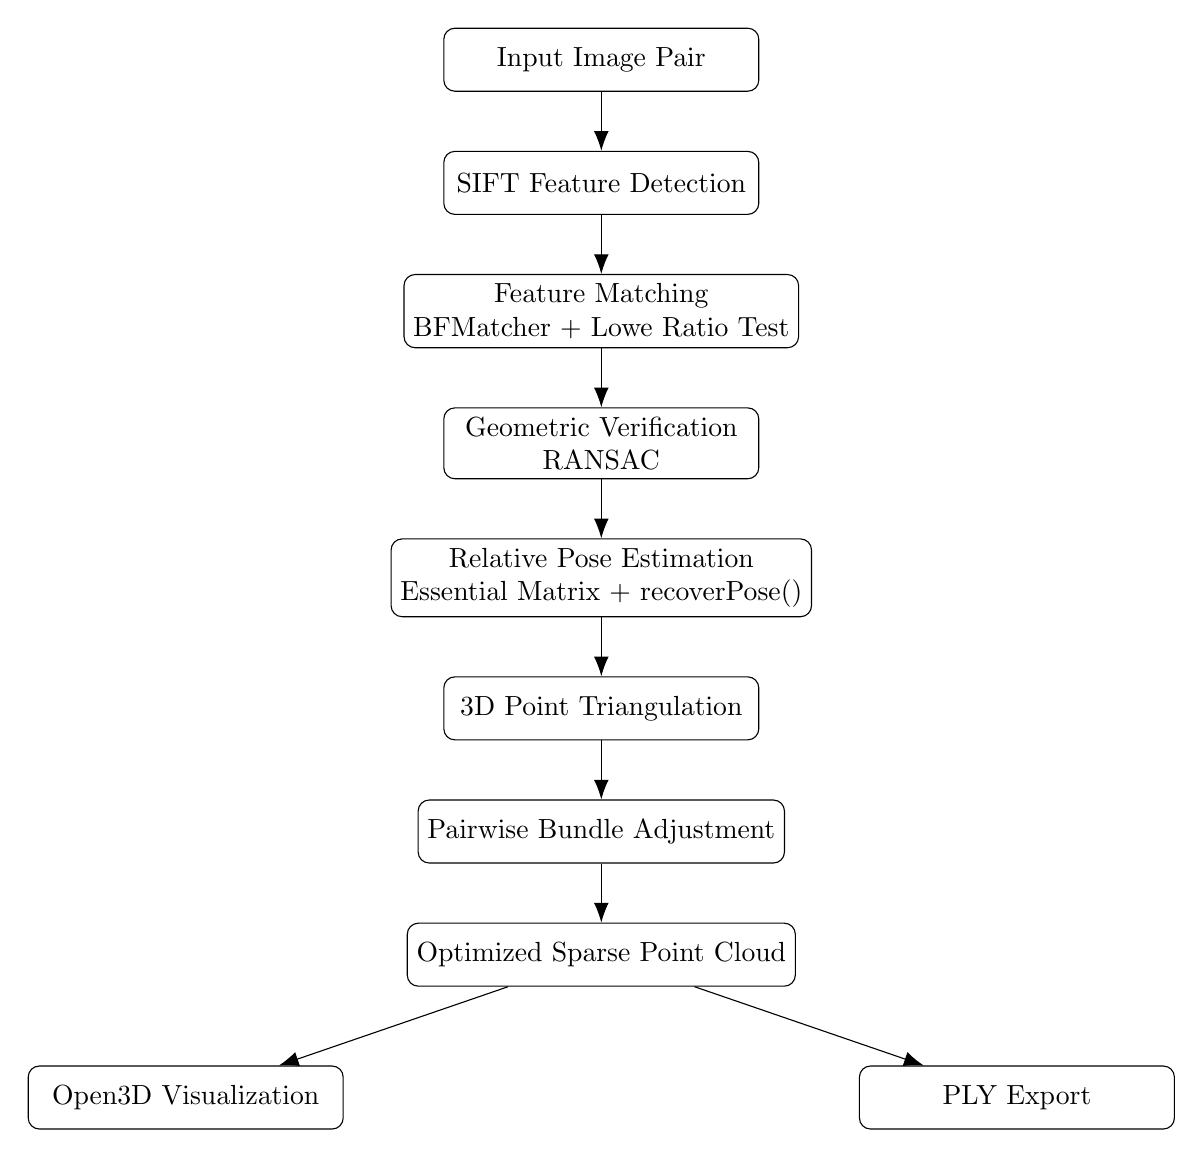
\begin{tikzpicture}[
    node distance=0.75cm,
    box/.style={
        draw,
        rounded corners,
        align=center,
        minimum width=4.0cm,
        minimum height=0.8cm
    },
    arrow/.style={
        -{Latex[length=2.5mm]}
    }
]

\node[box] (input) {Input Image Pair};

\node[box, below=of input] (features)
    {SIFT Feature Detection};

\node[box, below=of features] (matching)
    {Feature Matching\\BFMatcher + Lowe Ratio Test};

\node[box, below=of matching] (ransac)
    {Geometric Verification\\RANSAC};

\node[box, below=of ransac] (pose)
    {Relative Pose Estimation\\Essential Matrix + \code{recoverPose()}};

\node[box, below=of pose] (triangulation)
    {3D Point Triangulation};

\node[box, below=of triangulation] (ba)
    {Pairwise Bundle Adjustment};

\node[box, below=of ba] (output)
    {Optimized Sparse Point Cloud};

\node[box, below left=1.0cm and 0.8cm of output] (visualization)
    {Open3D Visualization};

\node[box, below right=1.0cm and 0.8cm of output] (export)
    {PLY Export};

\draw[arrow] (input) -- (features);
\draw[arrow] (features) -- (matching);
\draw[arrow] (matching) -- (ransac);
\draw[arrow] (ransac) -- (pose);
\draw[arrow] (pose) -- (triangulation);
\draw[arrow] (triangulation) -- (ba);
\draw[arrow] (ba) -- (output);
\draw[arrow] (output) -- (visualization);
\draw[arrow] (output) -- (export);

\end{tikzpicture}
}
\end{center}

The following subsections describe the individual components of this
pairwise reconstruction approach.

\subsubsection{Motivation for a Pairwise Approach}

Implementing a complete Structure from Motion system from low-level computer
vision primitives is considerably more complex than implementing the
individual reconstruction operations in isolation. While operations such as
feature detection, feature matching, essential matrix estimation, camera
pose recovery, and triangulation are available in OpenCV, a complete
multi-view SfM system additionally requires persistent management of camera
poses, feature observations, feature tracks, 3D landmarks, geometric
constraints, scale ambiguity, outlier rejection, and global optimization. A complete implementation would therefore require a substantially larger
architecture than the individual two-view reconstruction operations. For this reason, the feature-based implementation uses an independent
pairwise reconstruction model. Each consecutive image pair can be processed
without requiring information from previous or subsequent pairs. This makes
the individual reconstruction stages easier to inspect, test, and debug while
still providing the essential geometry of a two-view SfM problem. This decision does not imply that pairwise reconstruction is equivalent to a
complete multi-view SfM system. Rather, it provides a controlled intermediate
approach between individual two-view operations and a globally optimized
multi-view reconstruction. In particular, the implementation does not maintain a global camera
trajectory, persistent feature tracks, global landmarks, or a globally
consistent coordinate system. These aspects would be required for a complete
multi-view SfM implementation and were therefore outside the scope of this
specific reconstruction approach.

\subsubsection{Input and Pairwise Processing}

The reconstruction starts with two input images. At the current stage of the
project, images are loaded from a dataset stored on disk by the
\code{Camera} class. Each loaded image is represented by a \code{Frame} object.
The \code{Frame} stores the original image together with the information
generated during subsequent processing stages. This includes the image
filename and path, SIFT keypoints, SIFT descriptors, and camera-related
information associated with the reconstruction.

For an individual reconstruction, two frames are selected as an image pair.
For a sequence of images,

\begin{equation}
I_1, I_2, \ldots, I_N,
\end{equation}

the implementation can process consecutive pairs:

\begin{equation}
(I_1,I_2),
(I_2,I_3),
\ldots,
(I_{N-1},I_N).
\end{equation}

For a sequence containing $N$ images, this results in $N-1$ independent
image pairs. Each pair is reconstructed separately and produces its own
sparse point cloud. Although consecutive pairs share an image, their
reconstructions are not automatically aligned and therefore remain in
independent coordinate systems.

The use of the \code{Camera} abstraction keeps image acquisition separated
from the reconstruction stages. Consequently, replacing the current
dataset-based input with another image source does not require the
higher-level feature and geometry components to be redesigned.

The high-level \code{Reconstructor} orchestrates the geometric reconstruction
once a \code{MatchResult} has been prepared. The \code{MatchResult} contains
the two frames, their feature correspondences, geometrically valid inliers,
and the estimated relative camera pose. The \code{Reconstructor} passes this
information to the \code{Triangulator}, which reconstructs the valid
correspondences as 3D points and returns a \code{TriangulationResult}.
The resulting sparse \code{PointCloud} can be used directly after
triangulation without requiring Bundle Adjustment. If additional
optimization is desired, the triangulated points and their image
observations can instead be passed to the separate
\code{BundleAdjustment} component.
The \code{Reconstructor} does not maintain state across image pairs. No
global landmark database, camera trajectory, or persistent feature-track
structure is required. This allows individual pairs to be inspected and
evaluated independently while keeping the implementation simpler than a
complete multi-view SfM system.


\subsubsection{SIFT Feature Detection}

The first processing stage is the detection of local image features using
SIFT. Each image is processed independently. SIFT identifies distinctive local structures in an image and represents each
detected feature using a keypoint and a descriptor. The keypoint contains the
location and scale of the detected feature, while the descriptor encodes the
local image appearance. SIFT was selected because its feature representation is designed to be
relatively robust to changes in scale and rotation and to moderate changes
in illumination and viewpoint. This makes it suitable for establishing
correspondences between images acquired from different camera positions.
The detected keypoints and their corresponding descriptors are stored in the
respective \code{Frame} objects. These descriptors form the input to the
subsequent feature matching stage.
The feature detector is implemented as a separate
\code{FeatureDetector} component. It can operate on individual frames or on
a sequence of frames, allowing feature extraction to remain independent from
the subsequent geometric reconstruction.

\subsubsection{Feature Matching}

Once the SIFT descriptors have been extracted, descriptors from the two
images are compared to identify potential correspondences.
The implementation uses OpenCV's \code{BFMatcher}. For each descriptor in
the first image, the matcher searches for the closest descriptors in the
second image according to the descriptor distance.
The two nearest candidate matches are used by the \textbf{Lowe Ratio Test}.
A correspondence is accepted only when the best match is sufficiently better
than the second-best match. This removes many ambiguous correspondences in
regions where multiple image features have similar descriptors.
The resulting correspondences are stored in a \code{MatchResult}. The object
therefore becomes the main data structure passed from feature matching to the
geometric stages of the reconstruction.
At this point, however, the matches are only appearance-based
correspondences. Some may still be geometrically incorrect.

\subsubsection{Geometric Verification and Outlier Rejection}

Feature matching alone does not guarantee that all correspondences originate
from the same physical scene geometry. Incorrect correspondences can lead to
invalid camera poses and incorrect 3D points.
The implementation therefore performs geometric verification using
RANSAC-based estimation of the Essential Matrix.
The Essential Matrix describes the relative geometry between two calibrated
camera views. RANSAC repeatedly evaluates subsets of the available
correspondences and identifies a model that is consistent with the largest
possible set of observations.
The resulting correspondences are separated into geometrically consistent
\textit{inliers} and rejected \textit{outliers}. Only the inliers are used by
the subsequent pose estimation and triangulation stages.
The \code{MatchResult} stores both the matching information and the geometric
information required by the later stages, including the inlier matches and
the RANSAC mask.
This separation between appearance-based matching and geometric verification
is important because it allows the quality of the correspondences to be
evaluated before attempting 3D reconstruction.

\subsubsection{Relative Camera Pose Estimation}

After geometric verification, the relative camera motion between the two
images is estimated.
The Essential Matrix is computed using OpenCV's
\code{cv2.findEssentialMat()}, followed by relative pose recovery using
\code{cv2.recoverPose()}.
The recovered pose consists of a rotation matrix $R$ and a translation vector
$t$. The implementation uses the world-to-camera transformation convention

\begin{equation}
X_{\mathrm{camera}} =
R X_{\mathrm{world}} + t.
\end{equation}

For each pairwise reconstruction, the first camera defines the reference
coordinate system. Its pose is therefore

\begin{equation}
R_1 = I,
\qquad
t_1 = 0.
\end{equation}

The second camera is represented by the relative transformation estimated
from the image pair:

\begin{equation}
X_2 = R X_1 + t.
\end{equation}

The resulting rotation and translation are stored in the
\code{MatchResult} and are subsequently used by triangulation and, when
applicable, by dense stereo reconstruction.

An important limitation of monocular two-view reconstruction is that the
translation recovered from the Essential Matrix has an unknown absolute
scale. Consequently, the resulting 3D reconstruction is defined only up to
an arbitrary scale factor. The pairwise point cloud therefore describes the
relative geometry of the scene rather than providing metric dimensions.

\subsubsection{3D Point Triangulation}

Once the relative camera pose has been estimated, the geometrically valid
correspondences are triangulated to obtain their three-dimensional positions.
The projection matrix of the first camera is constructed as

\begin{equation}
P_1 = K
\begin{bmatrix}
I & 0
\end{bmatrix},
\end{equation}

while the second camera is represented as

\begin{equation}
P_2 = K
\begin{bmatrix}
R & t
\end{bmatrix},
\end{equation}

where $K$ denotes the camera intrinsic matrix.

The implementation uses OpenCV's
\code{cv2.triangulatePoints()} to reconstruct the 3D position of each
corresponding pair of image observations. The resulting homogeneous
coordinates are then converted into Euclidean 3D coordinates.
The \code{Triangulator} is responsible for this operation. It receives a
\code{MatchResult} together with the camera intrinsic matrix and returns a
\code{TriangulationResult}.
The result contains the reconstructed \code{PointCloud} as well as the
corresponding image observations from both images. Keeping the image
observations together with the reconstructed points is important because the
same correspondences are required later by Bundle Adjustment.
The triangulation stage additionally performs geometric validity checks.
Reconstructed points must satisfy the cheirality condition, meaning that they
must lie in front of both cameras. Points with excessive reprojection error
are also rejected.

For every retained point, the implementation therefore keeps the 3D
position, its observation in image 1, its observation in image 2, and its
optional RGB color information aligned by index.
RGB colors can be sampled from the first input image at the corresponding
feature locations. These colors are stored together with the reconstructed
points in the resulting \code{PointCloud}.

\subsubsection{Pairwise Bundle Adjustment}

Triangulation provides an initial estimate of the scene geometry, but both
the estimated camera pose and the reconstructed point positions are affected
by image measurement noise and errors in the initial geometric estimation.
Bundle Adjustment was therefore implemented as an additional optimization
stage that can be applied to the pairwise reconstruction when required.
However, it is not a mandatory component of the \code{Reconstructor} and is
kept separate from the main sparse reconstruction path.
This distinction was made because Bundle Adjustment can become
computationally expensive for image pairs producing a large number of
reconstructed points. During experimentation, some pairs required
considerable optimization time while providing only a limited improvement in
reprojection error. Consequently, applying Bundle Adjustment to every image
pair was not considered necessary or efficient.
When Bundle Adjustment is enabled, the first camera remains fixed as the
reference camera,

\begin{equation}
R_1 = I,
\qquad
t_1 = 0,
\end{equation}

while the optimization variables consist of the pose of the second camera
and the 3D coordinates of the reconstructed points.
For each 3D point, its estimated position is projected into both images.
The difference between the projected positions and the original feature
observations forms the reprojection residual.
The optimization therefore minimizes the combined reprojection error of the
two views. Conceptually, the objective is

\begin{equation}
\min
\left(
\sum_i
\left\|
\hat{x}_{1,i} - x_{1,i}
\right\|^2
+
\sum_i
\left\|
\hat{x}_{2,i} - x_{2,i}
\right\|^2
\right),
\end{equation}

where $x_{1,i}$ and $x_{2,i}$ are the observed image points and
$\hat{x}_{1,i}$ and $\hat{x}_{2,i}$ are their corresponding projected points.

The optimization is represented by the \code{BAProblem} class. This object
contains the second camera's rotation and translation, the reconstructed
3D points, and the corresponding observations in both images.
The \code{BundleAdjustment} class performs the numerical optimization using
SciPy's \code{least_squares}. A sparse Jacobian structure is used because an
individual observation depends only on the parameters of the second camera
and its corresponding 3D point. This avoids constructing unnecessary
dependencies between unrelated points.
When used, Bundle Adjustment transforms the initial triangulated
reconstruction into an optimized pairwise solution consisting of an
optimized camera pose and optimized 3D point positions. The resulting
3D
coordinates can then be represented as a \code{PointCloud} for visualization
or export.

\subsubsection{Point Cloud Representation and Output}

The reconstructed geometry is represented by the \code{PointCloud} class.
The point cloud contains the reconstructed 3D positions and, when available,
RGB colors.
The point positions are represented as an $N \times 3$ array,

\begin{equation}
\mathbf{P} =
\begin{bmatrix}
X_1 & Y_1 & Z_1\\
X_2 & Y_2 & Z_2\\
\vdots & \vdots & \vdots\\
X_N & Y_N & Z_N
\end{bmatrix}.
\end{equation}

The point cloud provides the main output of this reconstruction approach and
can be passed to subsequent processing stages. For qualitative inspection, the \code{Visualizer} converts the internal
representation into an Open3D point cloud and displays it interactively.
When RGB information is available, the point colors are preserved during
visualization. For persistent storage, the \code{PointCloudWriter} converts the internal
representation into an Open3D point cloud and exports it in PLY format. This
allows the reconstructed geometry to be inspected using external 3D
visualization and processing tools. It also prepares the point cloud for the subsequent registration module.


\subsubsection{Limitations of the Pairwise SIFT Reconstruction}

The pairwise SIFT reconstruction provides the fundamental geometry required
for two-view sparse reconstruction, but its deliberate simplification also
introduces limitations.
The implementation does not maintain a globally consistent camera trajectory
or coordinate system. Persistent feature tracks are not constructed across
multiple image pairs, and reconstructed landmarks are not associated between
different pairwise point clouds.
Consequently, two consecutive reconstructions can contain overlapping
physical regions while remaining independent in their coordinate systems.
The point cloud reconstructed from $(I_1,I_2)$ and the point cloud reconstructed
from $(I_2,I_3)$ are therefore not automatically expressed in a common global
frame.
Similarly, Bundle Adjustment is restricted to the individual image pair.
There is no global optimization capable of jointly refining all camera poses
and landmarks across an entire image sequence.

These limitations are a direct consequence of the chosen pairwise
architecture. They are acceptable for investigating individual reconstruction
stages and for producing local sparse geometry, but a globally consistent SfM
reconstruction would require additional components such as persistent feature
tracks, landmark management, camera-pose composition, inter-pair
registration, and global Bundle Adjustment.

\subsubsection{Evaluation on Palm Desert}

The pairwise SIFT reconstruction was initially evaluated using the Palm Desert
Micro dataset. The evaluation focused on the image pair
\code{DJI_0042.JPG} and \code{DJI_0043.JPG}. The results demonstrate that the
pipeline can establish a large number of reliable feature correspondences and
reconstruct a substantial sparse set of 3D points under favorable visual
conditions.

\begin{table}[H]
\centering
\caption{Results of the pairwise SIFT reconstruction on the Palm Desert image pair.}
\label{tab:palm_desert_sift_results}
\begin{tabular}{lr}
\toprule
Metric & Result \\
\midrule
Image 1 keypoints & 20,001 \\
Image 2 keypoints & 20,000 \\
Good matches & 3,476 \\
RANSAC inliers & 2,959 \\
Inlier ratio & 85.13\% \\
Reconstructed points & 2,959 \\
Reprojection error before BA & 0.1936 px \\
Reprojection error after BA & 0.1876 px \\
BA improvement & 3.11\% \\
\bottomrule
\end{tabular}
\end{table}

Bundle Adjustment reduced the mean reprojection error from 0.1936~px to
0.1876~px, corresponding to an improvement of 3.11\%. The optimization reached
the configured maximum number of function evaluations, so the improvement was
relatively limited despite the additional computational cost. Overall, the
Palm Desert experiment provided an initial validation of the pairwise
reconstruction workflow under conditions with sufficient visual structure.

\begin{figure}[H]
    \centering
    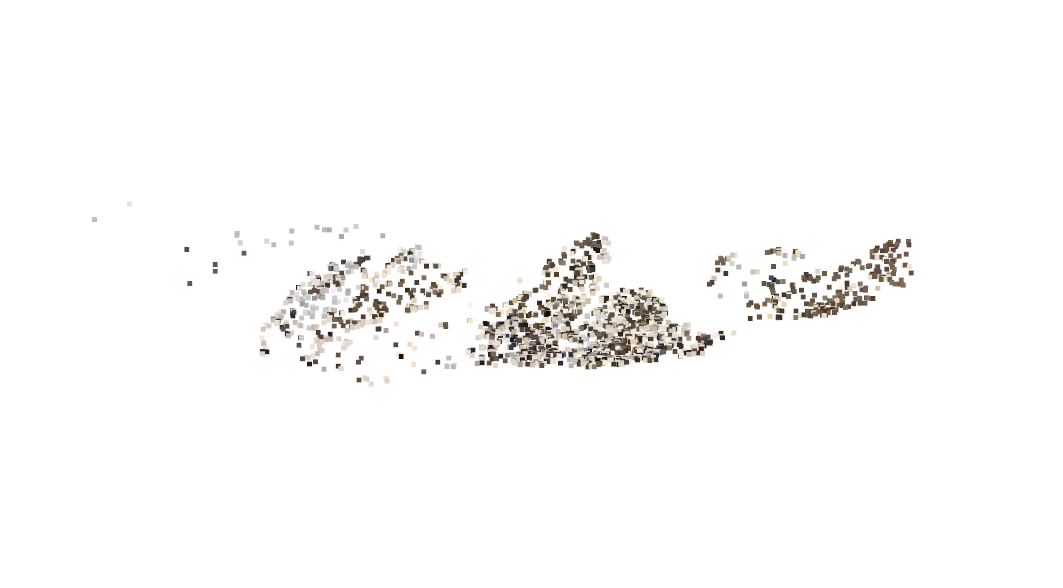
\includegraphics[width=\columnwidth]{3d reconstruction images/SIFT pairwise point cloud.png}
    \caption{Sparse 3D reconstruction obtained from the Palm Desert image pair.
    The reconstructed points capture recognizable scene structure, including
    the main hillside, while remaining distributed throughout the surrounding
    scene.}
    \label{fig:palm_desert_sparse_reconstruction}
\end{figure}

As shown in Figure~\ref{fig:palm_desert_sparse_reconstruction}, the resulting point cloud is sparse and does not form a continuous surface. Nevertheless, recognizable scene structure, including the main hillside visible in the input images, can be identified in the reconstruction. Additional reconstructed points are distributed across the surrounding scene, reflecting the feature-based nature of the approach rather than a dense surface reconstruction.


\subsubsection{Experimental Dense Reconstruction}

In addition to the sparse SIFT-based reconstruction, an experimental dense
stereo module was investigated. This module is intentionally treated as an
optional component rather than as a required stage of the main
feature-based reconstruction pipeline.

The \code{DenseReconstructor} operates on a single image pair and reuses the
relative rotation and translation already estimated during the feature-based
pipeline. The images are first downscaled to reduce computational cost and
their intrinsic matrix is scaled accordingly.
The pair is then rectified using OpenCV's
\code{cv2.stereoRectify()}, after which dense disparity is estimated using
\code{StereoSGBM}. The resulting disparity map is converted into 3D
coordinates using \code{cv2.reprojectImageTo3D()} and the reprojection matrix
obtained during rectification.
The module additionally performs validity checks and robust depth filtering
based on the Median Absolute Deviation (MAD). RGB values are sampled from the
rectified reference image and associated with the resulting 3D points.
This approach can produce substantially denser geometry than the sparse
feature-based reconstruction because depth is estimated over a large number
of image pixels rather than only at selected SIFT correspondences.

However, experiments showed that the dense reconstruction was not equally
reliable for all image pairs. Its quality depended strongly on the relative
camera motion, image overlap, scene texture, disparity distribution, and
quality of the estimated relative pose. Some pairs produced meaningful dense
geometry, whereas other pairs generated distorted or geometrically incorrect
structures.
For this reason, the dense stereo implementation remains experimental. It
was not considered necessary for the subsequent processing stages because
the sparse feature-based reconstruction already provides a set of 3D points
suitable for operations such as point cloud registration. The dense module
can therefore be evaluated or improved independently without becoming a
dependency of the main reconstruction workflow.

\subsection{OpenMVG/OpenMVS Reconstruction Pipeline}
\label{sec:openmvg_openmvs_pipeline}

To evaluate an established Structure-from-Motion (SfM) and multi-view stereo (MVS) reconstruction backend, a second reconstruction implementation was developed in \code{src_v2/}. Unlike the custom OpenCV-based reconstruction pipeline described previously, this implementation does not reproduce the individual SfM algorithms directly. Instead, Python provides the configuration, process orchestration, file management, and visualization interface, while the computational reconstruction stages are delegated to OpenMVG and OpenMVS. This pipeline is intentionally maintained as a separate reconstruction alternative. In particular, it is not an additional registration stage of the main DentaVision reconstruction pipeline: OpenMVG performs its own camera registration and SfM reconstruction as part of the established pipeline.

\subsubsection{Motivation for Using an Established SfM Pipeline}

The original reconstruction implementation was developed using OpenCV in order to expose and control the individual components of the SfM process, including SIFT feature extraction, feature matching, geometric verification, relative pose estimation, track construction, triangulation, landmark management, and bundle adjustment. This approach is useful for understanding the reconstruction process and for experimenting with individual algorithms, but it also requires substantial implementation and maintenance effort. In contrast, OpenMVG provides an established implementation of the complete sparse SfM workflow, including feature processing, matching, geometric filtering, camera estimation, triangulation, and optimization. The purpose of introducing OpenMVG was therefore not to replace the custom implementation, but to provide an alternative reconstruction backend in which the project could evaluate a more complete and established SfM implementation without having to reimplement the underlying reconstruction algorithms.

This distinction is also relevant when interpreting later experiments. Although OpenMVG provides the complete SfM framework, the feature extraction stage used by the project remains SIFT. Consequently, the use of an established SfM implementation does not eliminate limitations originating from the input features. In particular, scenes or images containing insufficient distinctive features can still present difficulties for feature matching and subsequent reconstruction. This makes the OpenMVG pipeline useful not only as a reconstruction backend, but also as an independent reference for evaluating the limitations of feature-based reconstruction.

\subsubsection{OpenMVG Pipeline}

The OpenMVG integration is implemented as a thin Python wrapper around the OpenMVG command-line applications. The project configuration is centralized in \code{src_v2/config/settings.py}, where the input image directory, OpenMVG installation, sensor-width database, output directories, feature extraction parameters, matching parameters, camera configuration, and SfM configuration are defined. Machine-dependent paths, including the input image directory and external software installations, are loaded from the project's \code{.env} file, while the OpenMVG executable directory and sensor-width database are derived from \code{OPENMVG_ROOT}. This keeps the reconstruction code independent of a particular installation path and allows camera- and dataset-dependent parameters to be changed without modifying the reconstruction pipeline itself.

\begin{figure}[H]
\centering
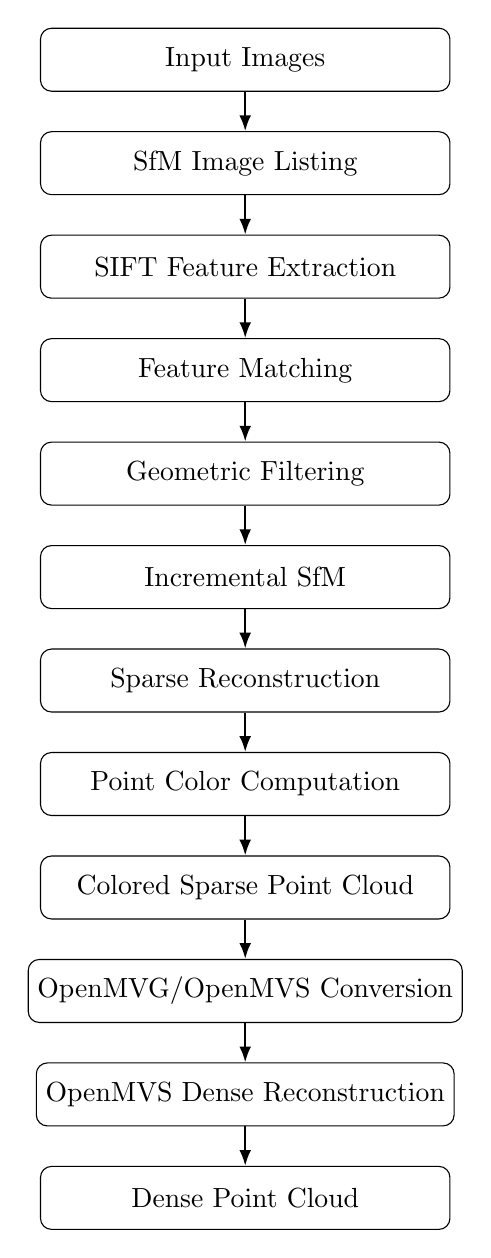
\begin{tikzpicture}[
node distance=0.5cm,
process/.style={
rectangle,
rounded corners,
draw,
align=center,
minimum width=5.2cm,
minimum height=0.8cm
},
arrow/.style={
-{Latex[length=2mm]},
thick
}
]

    \node[process] (input) {Input Images};
    \node[process, below=of input] (listing) {SfM Image Listing};
    \node[process, below=of listing] (features) {SIFT Feature Extraction};
    \node[process, below=of features] (matching) {Feature Matching};
    \node[process, below=of matching] (filtering) {Geometric Filtering};
    \node[process, below=of filtering] (sfm) {Incremental SfM};
    \node[process, below=of sfm] (sparse) {Sparse Reconstruction};
    \node[process, below=of sparse] (color) {Point Color Computation};
    \node[process, below=of color] (colored) {Colored Sparse Point Cloud};
    \node[process, below=of colored] (conversion) {OpenMVG/OpenMVS Conversion};
    \node[process, below=of conversion] (dense) {OpenMVS Dense Reconstruction};
    \node[process, below=of dense] (output) {Dense Point Cloud};

    \draw[arrow] (input) -- (listing);
    \draw[arrow] (listing) -- (features);
    \draw[arrow] (features) -- (matching);
    \draw[arrow] (matching) -- (filtering);
    \draw[arrow] (filtering) -- (sfm);
    \draw[arrow] (sfm) -- (sparse);
    \draw[arrow] (sparse) -- (color);
    \draw[arrow] (color) -- (colored);
    \draw[arrow] (colored) -- (conversion);
    \draw[arrow] (conversion) -- (dense);
    \draw[arrow] (dense) -- (output);

\end{tikzpicture}
\caption{End-to-end OpenMVG/OpenMVS reconstruction workflow.}
\label{fig:openmvg-openmvs-workflow}

\end{figure}

The sparse stage is coordinated by
\code{ReconstructionPipeline.run_sparse()}. First,
\code{openMVG_main_SfMInit_ImageListing} creates the initial
\code{sfm_data.json} from the input images and the configured camera
parameters. Camera-dependent values are centralized in
\code{settings.py}. When explicit intrinsic parameters are available, the
configured focal length and principal point are passed directly to OpenMVG.
If explicit focal-length information is not provided, OpenMVG can instead
use its sensor-width database together with the available image metadata to
initialize the camera intrinsics. This allows the same reconstruction
pipeline to be used with different cameras and image sets without requiring
changes to the reconstruction logic.


Feature extraction is then performed by
\code{openMVG_main_ComputeFeatures}. The project uses SIFT with the
\code{NORMAL} descriptor preset and configures 16 processing threads. The
resulting feature regions and descriptors are subsequently used by
\code{openMVG_main_ComputeMatches}, with a matching ratio configured in
\code{settings.py}. The resulting \code{matches.putative.bin} file contains
the initial feature correspondences.

These matches are subsequently passed to
\code{openMVG_main_GeometricFilter}, which uses the geometric model
configured by the project to remove correspondences that are inconsistent
with the estimated camera geometry. The selected geometric model is therefore
also treated as a configuration parameter rather than being hard-coded into
the reconstruction pipeline. The filtered correspondences are stored as
\code{matches.f.bin}.

The verified matches are then provided to
\code{openMVG_main_SfM}. The configured SfM engine is
\code{INCREMENTAL}, so OpenMVG progressively reconstructs the camera poses
and sparse 3D structure from the available image correspondences. The
reconstruction produces the OpenMVG SfM representation under
\code{output/openmvg/sfm/}, including \code{sfm_data.bin}. Finally,
\code{openMVG_main_ComputeSfM_DataColor} is used to generate the colored
sparse point cloud \code{cloud_and_poses.ply}. The visualization layer can
consume this point cloud without being coupled to the internal OpenMVG
representation.

The Python implementation deliberately keeps process execution separate from
reconstruction logic. The generic \code{run_command()} helper validates
executable paths, constructs and prints the generated command, and invokes
the external process using \code{subprocess.run(..., check=True)}.
Consequently, OpenMVG failures are propagated to the Python pipeline instead
of allowing subsequent stages to operate on invalid intermediate data. The
same abstraction is reused for the OpenMVS stage.

\subsubsection{Dense Reconstruction with OpenMVS}

OpenMVG provides the sparse reconstruction, whereas dense reconstruction is
delegated to OpenMVS. The implementation separates this process into two
independent operations: \code{prepare_dense()} converts the existing OpenMVG
reconstruction into an OpenMVS scene, while \code{run_dense()} performs the
actual dense reconstruction. This separation allows an existing scene to be
reused without repeating the sparse reconstruction or the scene conversion.

The scene preparation stage uses
\code{openMVG_main_openMVG2openMVS.exe}. Its primary input is the OpenMVG
reconstruction \code{sfm_data.bin}, and it generates
\code{output/openmvs/scene.mvs} together with the associated undistorted image
data. The resulting scene acts as the interface between the sparse OpenMVG
representation and the OpenMVS dense reconstruction stage. The implementation
also ensures that the image references required by the scene remain
accessible when OpenMVS loads the scene; the working directory used for the
dense reconstruction is therefore set to the directory containing the scene.

Dense reconstruction is performed by \code{DensifyPointCloud.exe}. The
generated point cloud is stored as
\code{output/openmvs/dense/pointcloud.ply}. The implementation supports CUDA
processing while retaining a CPU fallback. With the current configuration,
\code{OPENMVS_CUDA_DEVICE=None}, OpenMVS is first invoked with automatic GPU
selection (\code{-1}); if that attempt fails, the operation is retried using
CPU processing (\code{-2}). A specific CUDA device can alternatively be
configured, in which case the selected device is attempted first, followed by
automatic GPU selection and CPU processing. If a failed processing attempt
leaves an output file behind, that file is removed before the next attempt so
that an incomplete reconstruction cannot be mistaken for a successful
result.

The resulting architecture therefore separates the responsibilities of the
two reconstruction backends: OpenMVG performs feature-based sparse SfM and
produces camera poses and sparse 3D structure, while OpenMVS uses that
calibrated scene to generate a substantially denser point cloud. Camera
configuration and other dataset-dependent parameters remain external to the
reconstruction logic, allowing the same pipeline implementation to be reused
with different input image sets by modifying the project settings. Python
remains responsible for coordinating these stages and managing their
intermediate files rather than implementing the underlying SfM or MVS
algorithms.

\subsubsection{3D Reconstruction Results on the Palm Desert Dataset}
\label{sec:palm_desert_reconstruction_results}

The sparse reconstruction generated by OpenMVG was subsequently used as
input for dense reconstruction with OpenMVS. The input scene contained
21 calibrated images and 83,416 sparse 3D points. OpenMVS estimated
depth maps for all 21 views, enforced geometric consistency between
the views, and fused the resulting depth maps into a dense point cloud.
After depth-map fusion, filtering, and trimming to the estimated region
of interest, the final dense point cloud contained 1,753,190 3D points.
This corresponds to approximately 21 times the number of points in the
original sparse reconstruction, providing a substantially denser
representation of the reconstructed scene.

\begin{table}[H]
    \centering
    \caption{OpenMVG/MVS dense reconstruction results.}
    \label{tab:openmvs_dense_results}
    \begin{tabular}{lr}
        \hline
        \textbf{Metric} & \textbf{Result} \\
        \hline
        Calibrated images & 21 \\
        Sparse points & 83,416 \\
        Dense points & 1,753,190 \\
        Dense/Sparse ratio & $\approx 21\times$ \\
        \hline
    \end{tabular}
\end{table}

Figure~\ref{fig:sparse_dense_comparison} provides a visual comparison
between the sparse reconstruction produced by OpenMVG and the final
dense point cloud generated by OpenMVS. In the sparse reconstruction,
the green markers represent the estimated camera positions, whose
distribution reflects the relative camera motion recovered from the
image correspondences. The coherent camera trajectory provides a
visual indication that the feature tracks and pose estimation successfully
captured the camera movement throughout the sequence. The comparison
also illustrates the substantial increase in point density obtained
during the dense reconstruction stage while preserving the overall
geometry of the reconstructed scene.

\begin{figure}[H]
    \centering
    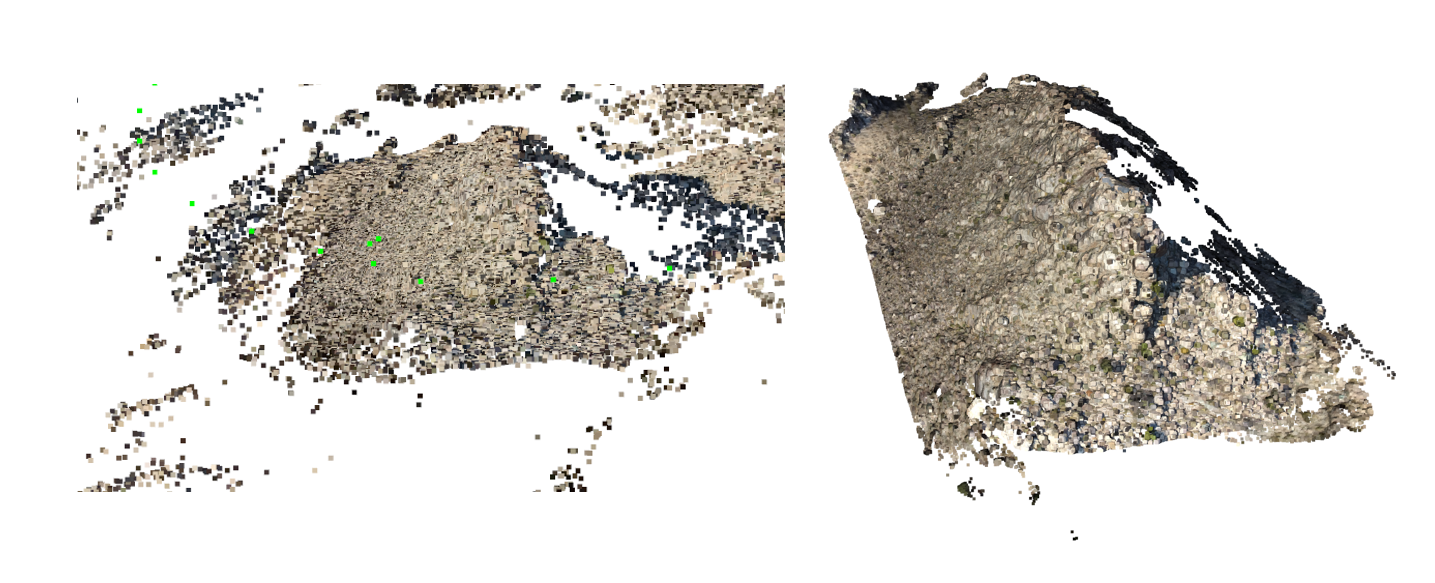
\includegraphics[width=\columnwidth]{3d reconstruction images/OpenMVG-MVS point clouds.png}
    \caption{Comparison between the sparse reconstruction generated by
    OpenMVG (left) and the dense point cloud generated by OpenMVS
    (right).}
    \label{fig:sparse_dense_comparison}
\end{figure}


\subsection{Evaluation on Low-Texture Scenes}

The feature-based reconstruction pipeline was initially developed and evaluated
using the Palm Desert Micro dataset provided through the OpenMVG image dataset
repository~\cite{openmvgImageDatasets}. While this dataset was suitable for
developing the reconstruction workflow, it did not sufficiently represent the
challenging visual conditions that may be encountered during dental
reconstruction, particularly in regions with limited distinctive visual
features. Therefore, an additional evaluation was required to investigate how
the current reconstruction approach behaves when the available image texture
is insufficient to establish a large number of reliable correspondences.

To investigate this limitation, additional experiments were performed using
the Middlebury Stereo 2006 datasets~\cite{scharstein2007learning,hirschmuller2007evaluation}.
The evaluation focused on four scenes with different visual characteristics:
\textit{Midd1}, \textit{Midd2}, \textit{Monopoly}, and \textit{Plastic}.
The four scenes were evaluated first using the implemented SIFT-based pairwise
pipeline and subsequently using OpenMVG for Structure-from-Motion. This
provided both a direct evaluation of the implemented feature-based approach
and an additional reference using an independent SfM implementation.

\subsubsection{Motivation for the Middlebury Dataset}

The Middlebury Stereo 2006 dataset was selected because it provides
well-established stereo scenes with controlled imaging conditions and
available ground-truth disparity data~\cite{scharstein2007learning,hirschmuller2007evaluation}.
The images are rectified, and the dataset provides stereo information for
specific image views, including \code{view1.png} and \code{view5.png}.
For the pairwise evaluation, these two views were used as an independent image
pair for each scene. Although the Middlebury scenes originate from a
multi-view stereo benchmark, the implemented pairwise experiment only receives
the selected two images. Consequently, the reconstruction performed by the
DentaVision pipeline remains a two-view reconstruction and does not use the
additional views available in the dataset.
The four selected scenes expose the reconstruction process to different levels
of available local image structure. In particular, the \textit{Plastic} scene
contains substantially fewer distinctive features than the other evaluated
scenes and therefore provides a useful stress case for feature-based
reconstruction.

The purpose of this experiment was not to evaluate dense stereo reconstruction
at this stage. Instead, the initial objective was to establish a baseline for
the existing feature-based reconstruction approach and determine whether a
lack of detectable and matchable image features could become a limiting factor
for sparse 3D reconstruction.

\subsubsection{SIFT Reconstruction on Middlebury Images}

The existing pairwise reconstruction pipeline was applied to
\code{view1.png} and \code{view5.png} for each of the four scenes without
changing its feature-based reconstruction architecture. For each image pair,
the number of detected SIFT keypoints, the number of matches remaining after
the Lowe ratio test, the number of RANSAC inliers, the resulting inlier ratio,
and the number of reconstructed 3D points were recorded.

The inlier ratio was computed as

\begin{equation}
\text{Inlier Ratio} =
\frac{\text{RANSAC Inliers}}
{\text{Good Matches}}
\times 100.
\end{equation}

An important change compared with the initial Middlebury experiment concerns
the camera calibration. The original project configuration had been defined
for the Palm Desert Micro dataset. The Middlebury experiments were therefore
rerun using the appropriate Middlebury camera parameters rather than the
Palm Desert calibration. This prevents the camera model from introducing an
additional source of error into the relative pose and triangulation stages.

The resulting measurements are summarized in
Table~\ref{tab:middlebury_sift_results}.

\begin{table}[H]
\centering
\caption{Results of the SIFT-based pairwise reconstruction on the Middlebury scenes.}
\label{tab:middlebury_sift_results}
\resizebox{\columnwidth}{!}{%
\begin{tabular}{lrrrrrr}
\toprule
Dataset & View 1 KP & View 5 KP & Good Matches &
Inliers & Inlier Ratio & 3D Points \\
\midrule
Midd1    & 621 & 610 & 344 & 311 & 90.41\% & 311 \\
Midd2    & 575 & 572 & 333 & 306 & 91.89\% & 306 \\
Monopoly & 684 & 701 & 414 & 287 & 69.32\% & 287 \\
Plastic  & 127 & 67  & 43  & 9   & 20.93\% & 9   \\
\bottomrule
\end{tabular}%
}
\end{table}

The first three scenes produced several hundred usable correspondences.
\textit{Midd1} produced 311 RANSAC inliers from 344 good descriptor matches,
corresponding to an inlier ratio of 90.41\%. Similarly, \textit{Midd2} produced
306 inliers from 333 good matches, resulting in an inlier ratio of 91.89\%.
The corresponding triangulation stages produced 311 and 306 reconstructed
points, respectively.
\textit{Monopoly} produced the largest number of candidate descriptor
matches, with 414 good matches. However, only 287 survived geometric
verification, resulting in a lower inlier ratio of 69.32\%. Nevertheless, the
resulting reconstruction still contained 287 3D points.
In contrast, \textit{Plastic} showed a substantial reduction in feature
availability. Only 127 keypoints were detected in \code{view1.png} and 67 in
\code{view5.png}. This resulted in only 43 good descriptor matches, of which
9 remained after RANSAC. The resulting inlier ratio was therefore only
20.93\%, and the triangulation stage produced only 9 3D points.

These results indicate that the degradation observed for \textit{Plastic}
occurs progressively throughout the feature-based reconstruction process. The
scene first provides substantially fewer detectable local features, which
limits the number of candidate descriptors and correspondences. The reduced
number of correspondences is then accompanied by lower geometric consistency,
ultimately leaving too few points for a substantial sparse reconstruction.

\subsubsection{OpenMVG and OpenMVS Evaluation}

To determine whether the observed limitations were specific to the implemented
pairwise reconstruction pipeline, the same four Middlebury scenes were also
processed using OpenMVG for Structure-from-Motion reconstruction. Unlike the
implemented pairwise pipeline, OpenMVG performs multi-view Structure-from-Motion
and therefore requires multiple images to estimate the camera motion and
reconstruct the scene. Consequently, all seven available views of each Middlebury
scene were used for the OpenMVG evaluation.
Therefore, the comparison is not intended to determine which implementation performs better, but rather to assess whether a multi-view SfM approach can provide sufficient sparse structure under the same challenging scene conditions. The SIFT-based experiment uses
only \code{view1.png} and \code{view5.png}, whereas OpenMVG uses the complete
seven-view sequence available for each scene. The two experiments are
therefore evaluated separately, with the OpenMVG results serving as an
additional assessment of the sparse reconstruction and its suitability as
input for subsequent dense reconstruction.
In particular, the number of OpenMVG tracks should not be interpreted as
directly comparable to the number of pairwise SIFT inliers. Instead, the
OpenMVG results were used to determine whether a sparse reconstruction could
be established and whether sufficient sparse structure was available for
subsequent dense reconstruction.

OpenMVG successfully produced a sparse reconstruction for all four evaluated
scenes. However, the amount of reconstructed structure varied considerably
between datasets. The recorded results are summarized in
Table~\ref{tab:middlebury_openmvg_results}.


\begin{table}[H]
\centering
\caption{OpenMVG sparse reconstruction results on the Middlebury scenes.}
\label{tab:middlebury_openmvg_results}
\resizebox{\columnwidth}{!}{%
\begin{tabular}{lrr}
\toprule
Dataset & Reconstructed Tracks / 3D Points & Calibrated Cameras \\
\midrule
Midd1    & 129 & 7 / 7 \\
Midd2    & 32  & 7 / 7 \\
Monopoly & 4   & 7 / 7 \\
Plastic  & 29  & 3 / 7 \\
\bottomrule
\end{tabular}%
}
\end{table}

The OpenMVG results demonstrate that successful camera calibration and sparse
reconstruction do not necessarily imply that a sufficiently dense set of
points is available for subsequent processing. For example, \textit{Midd1}
resulted in 129 reconstructed tracks with all seven input cameras calibrated,
whereas \textit{Monopoly} resulted in only four reconstructed tracks despite
all seven cameras being calibrated.
For \textit{Plastic}, OpenMVG reconstructed 29 tracks and calibrated three of
the seven input cameras. The corresponding residual statistics showed a mean
reprojection residual of approximately 0.18 pixels and a median of
approximately 0.10 pixels. These low residual values indicate that the
surviving tracks were geometrically consistent, but they do not imply
sufficient scene coverage.
The sparse reconstructions were subsequently passed to OpenMVS for dense
reconstruction. OpenMVS was not able to successfully complete the dense
reconstruction for the evaluated scenes. The observed behavior was
investigated through repeated tests to distinguish a possible implementation
problem from a limitation of the input reconstruction.
The experiments consistently showed that OpenMVG was able to produce a sparse
point cloud before the OpenMVS stage. Therefore, the observed OpenMVS failure
was not attributed to the absence of an OpenMVG reconstruction. Instead, the
results are consistent with the hypothesis that the sparse reconstructions
contained too few reliable points and tracks to provide sufficient geometric
support for successful densification.

This interpretation should be considered an experimental observation rather
than a formally isolated causal result. The experiments did not independently
vary the number of sparse points while keeping all other conditions constant.
Nevertheless, the combination of sparse OpenMVG reconstructions and the
subsequent failure of dense reconstruction provides evidence that insufficient
sparse scene structure is a plausible limitation of the SfM-to-MVS approach
for these scenes.

\subsubsection{Implications for Dental Reconstruction}

The Middlebury experiments demonstrate an important limitation of
feature-based sparse reconstruction: its performance depends strongly on the
availability of distinctive and repeatable visual features.
These findings are relevant to dental reconstruction because dental surfaces
cannot be assumed to provide uniformly distinctive local image features.
Regions with limited local texture may result in fewer reliable feature
correspondences, while specular reflections and other appearance variations
can further complicate feature matching. A reconstruction approach that relies
exclusively on sparse feature correspondences may therefore provide
insufficient spatial coverage in some regions of the scene.

The experiments do not establish that SIFT or feature-based reconstruction is
generally unsuitable for dental images. Instead, they identify a specific
limitation of the current approach: reconstruction quality and coverage can
degrade substantially when the available visual features are insufficient.
Consequently, the Middlebury evaluation established the SIFT-based sparse
reconstruction as a baseline and motivated the investigation of dense stereo
correspondence as a complementary reconstruction strategy. The subsequent
evaluation of StereoSGBM is therefore presented separately, with the
\textit{Plastic} scene providing a particularly useful test case for dense
stereo because ground-truth disparity is available.

\subsection{Stereo Reconstruction with SGBM}

As an alternative to the feature-based reconstruction pipeline, DentaVision includes a dense stereo reconstruction approach based on OpenCV's Stereo Semi-Global Block Matching (StereoSGBM). This approach was evaluated using the Middlebury 2006 Plastic stereo dataset, which provides a calibrated and already rectified stereo pair together with a ground-truth disparity map. The stereo implementation is organized into separate components for disparity estimation, disparity validation, depth computation, and 3D point cloud reconstruction.

\subsubsection{StereoSGBM Implementation}

The disparity estimation stage is implemented by the \code{StereoMatcher} class in \longcode{src/pipeline/stereo/matcher.py}. It encapsulates OpenCV's \code{cv2.StereoSGBM_create()} and computes a dense disparity map from a pair of rectified stereo images. The implementation accepts either grayscale or BGR images. BGR images are converted to grayscale before matching, while grayscale images are used directly. The two input images are required to have identical spatial dimensions.

The matcher exposes the main StereoSGBM parameters through its constructor. The default configuration uses a minimum disparity of 0 and searches 128 disparity levels. The matching block size is set to 5 pixels, with a uniqueness ratio of 10, a speckle window size of 100 pixels, a speckle range of 2, and a maximum left-right disparity difference of 1 pixel. The implementation uses the \code{STEREO_SGBM_MODE_SGBM_3WAY} mode. The smoothness penalties are derived from the block size as \(P_1=8b^2\) and \(P_2=32b^2\), where \(b\) denotes the selected block size. Input validation also ensures that the number of disparity levels is a positive multiple of 16 and that the block size is a positive odd number.

OpenCV internally stores StereoSGBM disparity values with a fixed scale factor of 16. Therefore, the implementation converts the output to floating-point pixel units by dividing the computed disparity map by 16. The resulting array has the same spatial resolution as the input images and is represented using \code{float32}.

For the Middlebury evaluation, the images used were the ThirdSize versions of \code{view1.png} and \code{view5.png}, with a resolution of \(423\times370\) pixels. The dataset images are already rectified and have radial distortion removed, so no additional stereo rectification or distortion correction is performed by the reconstruction pipeline. The corresponding camera configuration is therefore derived directly from the parameters provided by the dataset. The original focal length of 3740 pixels is scaled according to the ThirdSize image resolution, while the stereo baseline is 160 mm. The principal point is set to the center of the \(423\times370\) image. A corresponding \(4\times4\) reprojection matrix \(Q\) is also defined for the Middlebury stereo geometry and supplied to the 3D reconstruction component.

\subsubsection{Disparity Validation and Depth Reconstruction}

After disparity estimation, the resulting map is passed to the \code{StereoValidator}. This component is intentionally separated from the reconstruction stages and currently performs two basic validity checks: disparity values must be finite and strictly greater than zero. The result is a boolean validity mask with the same dimensions as the disparity map. This separation allows additional validation strategies, such as left-right consistency checks, to be introduced later without changing the depth or point cloud reconstruction components.

The validated disparity can subsequently be used to estimate depth. This functionality is implemented by the \code{DepthReconstructor}, which applies the stereo depth relationship \(Z=fB/d\) to all finite, positive disparity values. Invalid values are assigned a depth of zero. The focal length and baseline are provided to the component externally, and the resulting depth map uses the same physical unit as the supplied baseline.

For the Middlebury dataset, an additional disparity offset has to be considered during reconstruction. The ThirdSize images are cropped versions of the original images, and the dataset specifies a minimum disparity value of \(d_{\min}=280\) pixels. Consequently, the disparity estimated by StereoSGBM is offset before it is used for the Middlebury reconstruction:

\begin{equation}
d_{\mathrm{reconstruction}}
=
d_{\mathrm{SGBM}}
+
d_{\min}.
\label{eq:disparity_reconstruction}
\end{equation}

With the baseline expressed in millimeters, the resulting depth values are correspondingly expressed in millimeters.

The final 3D reconstruction is handled by the \code{StereoReconstructor}. Rather than explicitly computing the three-dimensional coordinates from individual image coordinates and depth values, this component uses OpenCV's \code{cv2.reprojectImageTo3D()} function. The function receives the reconstruction disparity and an externally supplied \(4\times4\) reprojection matrix \(Q\). Keeping \(Q\) outside the reconstruction class makes the component independent of a specific camera or dataset.

The complete disparity map is first reprojected into 3D space. The validation mask is then used to select only the pixels considered valid for reconstruction. Any resulting 3D coordinates that are not finite are discarded. The corresponding colors are obtained from the left stereo image, converted from BGR to RGB, and normalized to the range \([0,1]\). The resulting points and colors are stored in the common \code{PointCloud} representation used by the rest of the reconstruction pipeline.

The resulting processing flow can therefore be summarized as:

\begin{figure}[H]
    \centering
    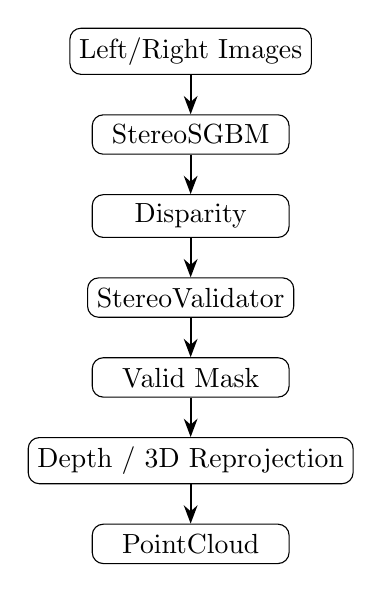
\begin{tikzpicture}[
        node distance=0.5cm,
        block/.style={
            draw,
            rounded corners,
            align=center,
            minimum height=0.5cm,
            minimum width=2.5cm
        },
        arrow/.style={
            -{Stealth},
            thick
        }
    ]

        \node[block] (input) {Left/Right Images};
        \node[block, below=of input] (sgbm) {StereoSGBM};
        \node[block, below=of sgbm] (disparity) {Disparity};
        \node[block, below=of disparity] (validator) {StereoValidator};
        \node[block, below=of validator] (mask) {Valid Mask};
        \node[block, below=of mask] (depth) {Depth / 3D Reprojection};
        \node[block, below=of depth] (pointcloud) {PointCloud};

        \draw[arrow] (input) -- (sgbm);
        \draw[arrow] (sgbm) -- (disparity);
        \draw[arrow] (disparity) -- (validator);
        \draw[arrow] (validator) -- (mask);
        \draw[arrow] (mask) -- (depth);
        \draw[arrow] (depth) -- (pointcloud);

    \end{tikzpicture}
    \caption{Dense stereo reconstruction pipeline using StereoSGBM.}
    \label{fig:sgbm_pipeline}
\end{figure}

\subsubsection{Quantitative and Qualitative Results}

The StereoSGBM implementation was evaluated quantitatively against the ground-truth disparity provided by the Middlebury Plastic dataset. Three matching block sizes, 3, 5, and 7 pixels, were tested while keeping the remaining StereoSGBM parameters unchanged. The results are summarized in Table~\ref{tab:stereosgbm_block_sizes}.

\begin{table}[H]
\centering
\caption{StereoSGBM disparity accuracy for different block sizes on the Middlebury Plastic dataset.}
\label{tab:stereosgbm_block_sizes}
\resizebox{\columnwidth}{!}{%
\begin{tabular}{c|ccccc}
\hline
Block size & MAE (px) & Median AE (px) & $>1$ px & $>2$ px & $>5$ px \\
\hline
3 & 2.81 & 0.60 & 37.78\% & 27.27\% & 18.64\% \\
5 & 2.91 & 0.60 & 39.06\% & 29.23\% & 20.13\% \\
7 & \textbf{2.66} & 0.60 & 38.30\% & 28.27\% & \textbf{18.91\%} \\
\hline
\end{tabular}%
}
\end{table}

Among the tested configurations, a block size of 7 produced the lowest mean absolute error of 2.66 pixels and was therefore selected for the subsequent reconstruction. Although the improvement over the other configurations was small, it provided the best quantitative result, while the median absolute error remained unchanged at 0.60 pixels. Nevertheless, the disparity estimates still contained a considerable number of local errors: \(38.30\%\) of the valid comparison pixels had an absolute error greater than 1 pixel, and \(18.91\%\) exceeded 5 pixels.

For the subsequent reconstruction, the selected configuration produced a disparity map of \(370\times423\) pixels. The \code{StereoValidator} classified \(45.94\%\) of the image pixels as valid, excluding disparities that were non-finite or not strictly positive. This value reflects the validity criterion of the implementation rather than the accuracy of the disparity estimates.
After applying the Middlebury \(d_{\min}\) offset, the reconstructed disparity values corresponded to depths between approximately 1.73 m and 2.13 m, with a mean depth of 1.84 m. The reprojection produced 71,904 valid 3D points, with no additional point loss caused by non-finite coordinates. Thus, the resulting point cloud contained one 3D point for each valid disparity pixel in this evaluation.


\begin{figure}[H]
\centering
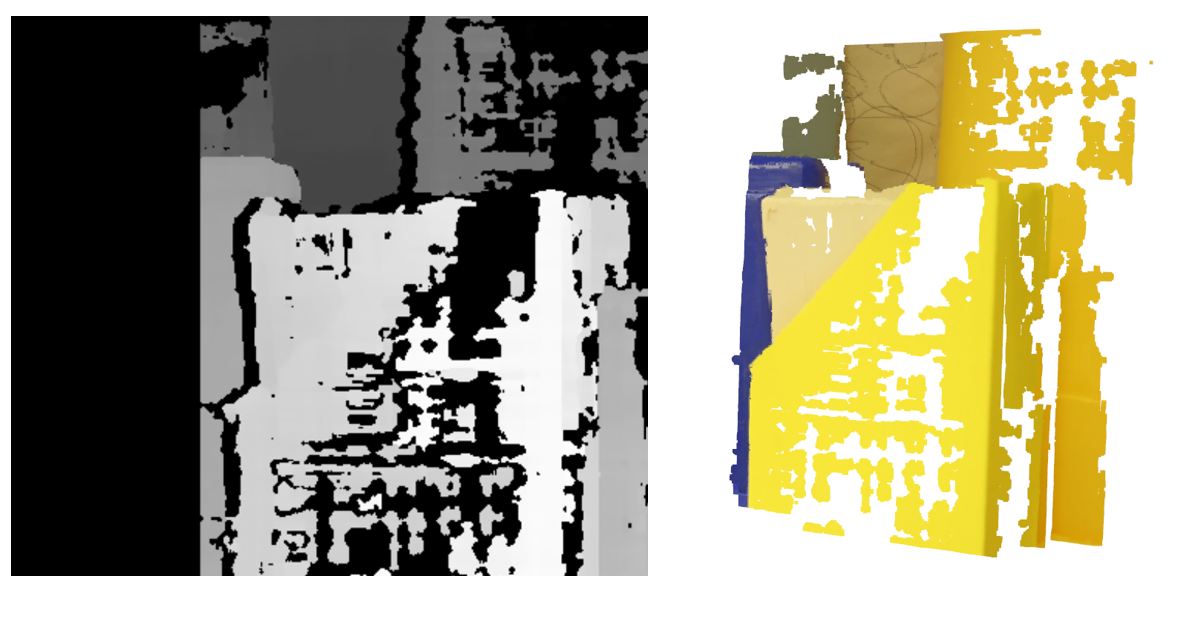
\includegraphics[width=0.8\linewidth]{3d reconstruction images/SGBM output.png}
\caption{Dense stereo reconstruction of the Middlebury Plastic
ThirdSize image pair using StereoSGBM. The left image shows the
estimated disparity map, while the right image shows the corresponding
colored 3D point cloud reconstructed from the disparity.}
\label{fig:sgbm_disparity_pointcloud}
\end{figure}


As shown in Figure~\ref{fig:sgbm_disparity_pointcloud}, the estimated
disparity provides a dense representation of the scene's depth structure.
The main regions of the scene are recovered consistently, while some
areas contain invalid or missing disparity values. These regions indicate
locations where a reliable disparity estimate was not obtained. The
corresponding colored point cloud provides a three-dimensional
representation of the reconstructed scene while retaining the color
information. The recovered spatial structure is consistent with the
disparity estimation, although the density and completeness of the point
cloud depend directly on the reliability and spatial coverage of the
underlying disparity map.


\subsection{IGEV Stereo Reconstruction with OpenStereo}

\subsubsection{Overview}

The project integrates the IGEV stereo matching model through the external
OpenStereo framework to provide dense stereo disparity for 3D reconstruction.
Unlike the custom StereoSGBM implementation, IGEV is a pretrained
deep-learning stereo model. OpenStereo provides the IGEV implementation,
configuration, preprocessing, and inference functionality, while DentaVision
integrates its disparity output into the existing stereo reconstruction
pipeline.

\subsubsection{Motivation for Using OpenStereo}

The project uses IGEV through the OpenStereo framework rather than integrating
the original IGEV implementation directly.
The main reason for this choice is to keep the stereo matching component
flexible. OpenStereo provides a common framework for multiple stereo matching
models, allowing the project to use IGEV while keeping the integration
independent from a single model implementation.
This makes it possible to evaluate or replace the stereo matching method in
the future with other models supported by OpenStereo without requiring major
changes to the downstream reconstruction pipeline. The
\code{IGEVMatcher} isolates the framework-specific details, while the rest of
the pipeline only receives a dense disparity map.
Therefore, OpenStereo is used not only as the implementation source for IGEV,
but also as an abstraction layer that keeps the project open to additional
deep-learning stereo models in the future.

\subsubsection{Preprocessing and Padding}

The evaluation transform configured by OpenStereo can pad the input images to
dimensions compatible with the IGEV network. The matcher stores the original
image dimensions before preprocessing and removes the added padding after
inference.
For the configured transform, padding is added to the top and right sides.
Consequently, the original image corresponds to the upper-left region of the
model output. The matcher removes the padded rows from the top and the padded
columns from the right before returning the disparity.
The final disparity therefore has exactly the same dimensions as the original
input image. This is required so that the disparity remains spatially aligned
with the left image during subsequent validation and 3D reconstruction.

\subsubsection{OpenStereo Integration}

OpenStereo is kept as an external dependency and is not included in the
DentaVision source tree. Both OpenStereo and IGEV checkpoint are configured through the \code{.env} file. They have separate variables, which keeps the OpenStereo installation and the pretrained checkpoint independent from each other.

The integration is implemented in
\code{src/pipeline/stereo/igev_matcher.py}. The \code{IGEVMatcher} acts as an
adapter between the DentaVision stereo pipeline and OpenStereo. During
initialization, it loads the OpenStereo configuration, assigns the configured
checkpoint, builds the IGEV model through OpenStereo, and creates the
evaluation transform defined by the selected configuration.
For each stereo pair, \code{compute()} validates the input images and their
dimensions, converts the OpenCV BGR images to RGB, and applies the OpenStereo
evaluation transform. The resulting tensors are batched and moved to the
selected device before IGEV inference is performed without gradient
computation. The predicted \code{disp_pred} is then extracted, converted to a
\code{float32} NumPy array, and any padding introduced by the OpenStereo
transform is removed before returning the disparity at the original image
resolution.


The matcher therefore exposes a simple interface to the rest of the project:

\begin{center}
\resizebox{\columnwidth}{!}{
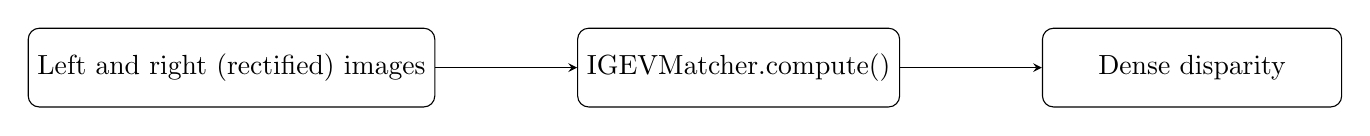
\begin{tikzpicture}[
    node distance=1.2cm,
    box/.style={
        rectangle,
        draw,
        rounded corners,
        align=center,
        minimum width=3.8cm,
        minimum height= 1cm
    },
    arrow/.style={->, >=stealth}
]

\node[box] (input) {Left and right (rectified) images};
\node[box, right=1.8cm of input] (matcher)
{\code{IGEVMatcher.compute()}};
\node[box, right=1.8cm of matcher] (output)
{Dense disparity};

\draw[arrow] (input) -- (matcher);
\draw[arrow] (matcher) -- (output);

\end{tikzpicture}
}
\end{center}

The rest of the reconstruction pipeline therefore does not need to interact
directly with the OpenStereo trainer or the IGEV model implementation.


\subsubsection{Middlebury Evaluation}

The IGEV implementation was evaluated using the Plastic stereo pair from the
Middlebury dataset. The images have a resolution of $423 \times 370$ pixels.
The Middlebury ThirdSize ground-truth disparity is stored with a scale factor
of three. Therefore, the raw ground-truth values are divided by three before
comparison with the IGEV prediction.

The evaluation produced the following results:

\begin{table}[ht]
\centering
\caption{IGEV disparity accuracy on the Middlebury Plastic dataset.}
\label{tab:igev_disparity_accuracy}
\begin{tabular}{l r}
\hline
Metric & Result \\
\hline
Disparity minimum & 17.73 px \\
Disparity maximum & 64.95 px \\
Disparity mean & 45.10 px \\
Disparity median & 44.11 px \\
\hline
Valid comparison pixels & 156267 \\
Mean absolute error & 0.42 px \\
Median absolute error & 0.27 px \\
Maximum absolute error & 24.82 px \\
Mean signed error & -0.17 px \\
Median signed error & -0.12 px \\
Absolute error $> 1$ px & 7.64\% \\
Absolute error $> 2$ px & 1.05\% \\
Absolute error $> 5$ px & 0.20\% \\
\hline
\end{tabular}
\end{table}

The mean absolute error of $0.42$ pixels and median absolute error of
$0.27$ pixels show a close agreement between the IGEV prediction and the
Middlebury ground truth. Only $0.27\%$ of the compared pixels have an
absolute error greater than five pixels.

\subsubsection{Dense Reconstruction}

The predicted disparity was passed to the existing
\code{StereoValidator}, \code{DepthReconstructor}, and
\code{StereoReconstructor} components.
The current validation accepted all 156510 pixels,
resulting in a validity ratio of $100.00\%$.
The resulting depth values ranged from $3070.72$ mm to $11249.35$ mm, with a
mean of $5050.46$ mm and a median of $4522.90$ mm.
The final 3D reconstruction contained 156510 points. The point coordinates
have shape $(156510, 3)$ and the corresponding point colors have shape
$(156510, 3)$.

Figure~\ref{fig:igev_disparity_pointcloud} provides a visual representation
of the dense stereo result and the resulting 3D reconstruction. The
disparity captures the main depth structure of the scene, which is reflected
in the spatial organization of the reconstructed point cloud. Qualitatively,
the reconstruction appears largely complete, with few visible gaps or
inconsistencies relative to the scene represented in the input stereo pair.
The resulting point cloud therefore provides a coherent representation of
the observed scene structure.

\begin{figure}[H]
\centering
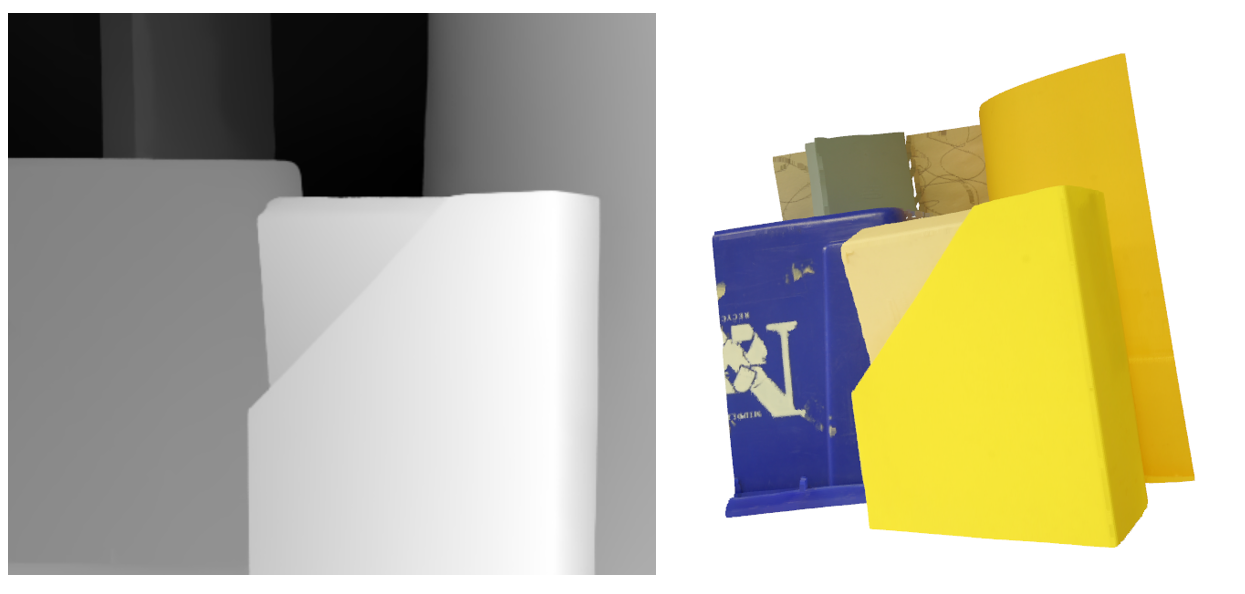
\includegraphics[width=0.8\linewidth]{3d reconstruction images/IGEV output.png}
\caption{Dense stereo result and 3D reconstruction obtained with IGEV
on the Middlebury Plastic stereo pair. The left image shows the
estimated disparity map, while the right image shows the corresponding
colored 3D point cloud reconstructed from the disparity.}
\label{fig:igev_disparity_pointcloud}
\end{figure}

The IGEV integration therefore provides a dense stereo backend that can be
used with the existing validation, depth reconstruction, and 3D
reconstruction components without requiring model-specific processing in
those stages.

\subsection{Comparative Evaluation}
\label{sec:comparative_evaluation}

The evaluated reconstruction approaches differ in their input requirements
and reconstruction principles. Consequently, a single quantitative metric
cannot be applied fairly to all four methods. The pairwise SIFT and
OpenMVG/OpenMVS approaches are instead considered primarily in terms of
their behavior and limitations observed during the low-texture evaluation,
while StereoSGBM and IGEV allow a direct quantitative comparison because
both estimate dense disparity from the same calibrated stereo pair.

\begin{table}[H]
    \centering
    \caption{Quantitative comparison of dense stereo reconstruction on the
    Middlebury Plastic dataset. For StereoSGBM, the results correspond to
    the best-performing block size of 7.}
    \label{tab:stereo_comparison}
    \begin{tabular}{lcc}
        \hline
        \textbf{Metric} & \textbf{StereoSGBM} & \textbf{IGEV} \\
        \hline
        Block size & 7 & -- \\
        Mean absolute error (px) & 2.66 & \textbf{0.42} \\
        Median absolute error (px) & 0.60 & \textbf{0.27} \\
        Error $>1$ px & 38.30\% & \textbf{7.64\%} \\
        Error $>2$ px & 28.27\% & \textbf{1.05\%} \\
        Error $>5$ px & 18.91\% & \textbf{0.20\%} \\
        \hline
    \end{tabular}
\end{table}

The quantitative evaluation shows a clear advantage of IGEV over
StereoSGBM on the Middlebury Plastic scene. IGEV achieved a mean absolute
disparity error of 0.42~px compared with 2.91~px for StereoSGBM, while the
median error decreased from 0.60~px to 0.27~px. The IGEV results also show
that only 0.27\% of the evaluated pixels have an absolute disparity error
greater than 5~px. Both methods produced disparity maps with comparable
overall disparity statistics, indicating that the difference is primarily
in the accuracy of the estimated disparity rather than in the recovered
disparity range.

More broadly, the experiments show that feature-based approaches can
provide useful sparse reconstructions when sufficient visual structure is
available, as demonstrated by the initial Palm Desert evaluation.
However, the Middlebury experiments exposed substantial limitations under
low-texture conditions. The use of OpenMVG's multi-view SfM formulation
does not fundamentally remove this limitation, since it still relies on
reliable image correspondences to establish the scene geometry. In
contrast, dense stereo methods directly estimate disparity from the
calibrated stereo pair and therefore do not require a sparse
feature-based scene representation. Between the two evaluated stereo
approaches, IGEV achieved substantially lower disparity error than
StereoSGBM on the Plastic scene and provided the most promising results
for the targeted stereo reconstruction scenario.

\subsection{Conclusion}

This work investigated several approaches for reconstructing three-dimensional geometry from image data within the DentaVision project. Feature-based reconstruction using SIFT provided a functional sparse reconstruction pipeline and demonstrated that reliable camera motion and 3D points can be obtained when sufficient visual structure is available. However, the experiments on the low-texture Middlebury Plastic dataset revealed clear limitations of feature-based methods in regions with little distinctive texture. The use of OpenMVG and OpenMVS confirmed that a multi-view SfM pipeline does not fully overcome this limitation when the input images do not provide sufficient visual correspondences.
Dense stereo methods proved more suitable for the low-texture scenario. StereoSGBM was able to produce a dense disparity map, but its accuracy remained limited, particularly in regions where local image structure was insufficient. In contrast, the IGEV-based stereo approach achieved substantially lower disparity errors on the same calibrated Middlebury stereo pair.
The Plastic stereo pair is particularly relevant to the intended DentaVision application because its predominantly low-texture surfaces provide a scenario that is more representative of the visual characteristics expected from dental surfaces than the highly textured Palm Desert dataset. Based on its strong quantitative performance in this evaluation, IGEV will be used as the basis for the stereo matching component of the DentaVision reconstruction pipeline. Its ability to produce accurate dense disparity in this challenging low-texture scenario makes it a particularly suitable approach for the intended application.
\chapterbreak

\section{title}
\sectionauthors{Marvin Kraus}

\subsection{Overview and Scope}
\label{sec:marvin-overview}

This part of the project covers two consecutive processing stages: rigid registration of partially overlapping dental point clouds and surface reconstruction of the resulting merged point cloud. Image acquisition and point-cloud generation are handled by the preceding reconstruction stage; the present contribution starts with multiple point-cloud fragments in different local coordinate systems and ends with an explicit triangular surface model.

The development was deliberately organized as an experimental selection process rather than around a single preselected algorithm. Five pairwise registration methods were first screened on controlled synthetic dental-like data. The most promising approaches were then re-evaluated on five distinct dental model sets comprising ten upper- and lower-jaw STL meshes. Each mesh was sampled into a point cloud, split into overlapping fragments, and displaced by known rigid motions. This broader validation stage changed the final registration decision from Fast Global Registration (FGR) to RANSAC-based global registration. Surface reconstruction was evaluated in the same way: Poisson Surface Reconstruction and the Ball Pivoting Algorithm (BPA) were first compared on the synthetic dataset and then re-evaluated across all ten realistic jaw meshes.

\begin{figure*}[!t]
    \centering
    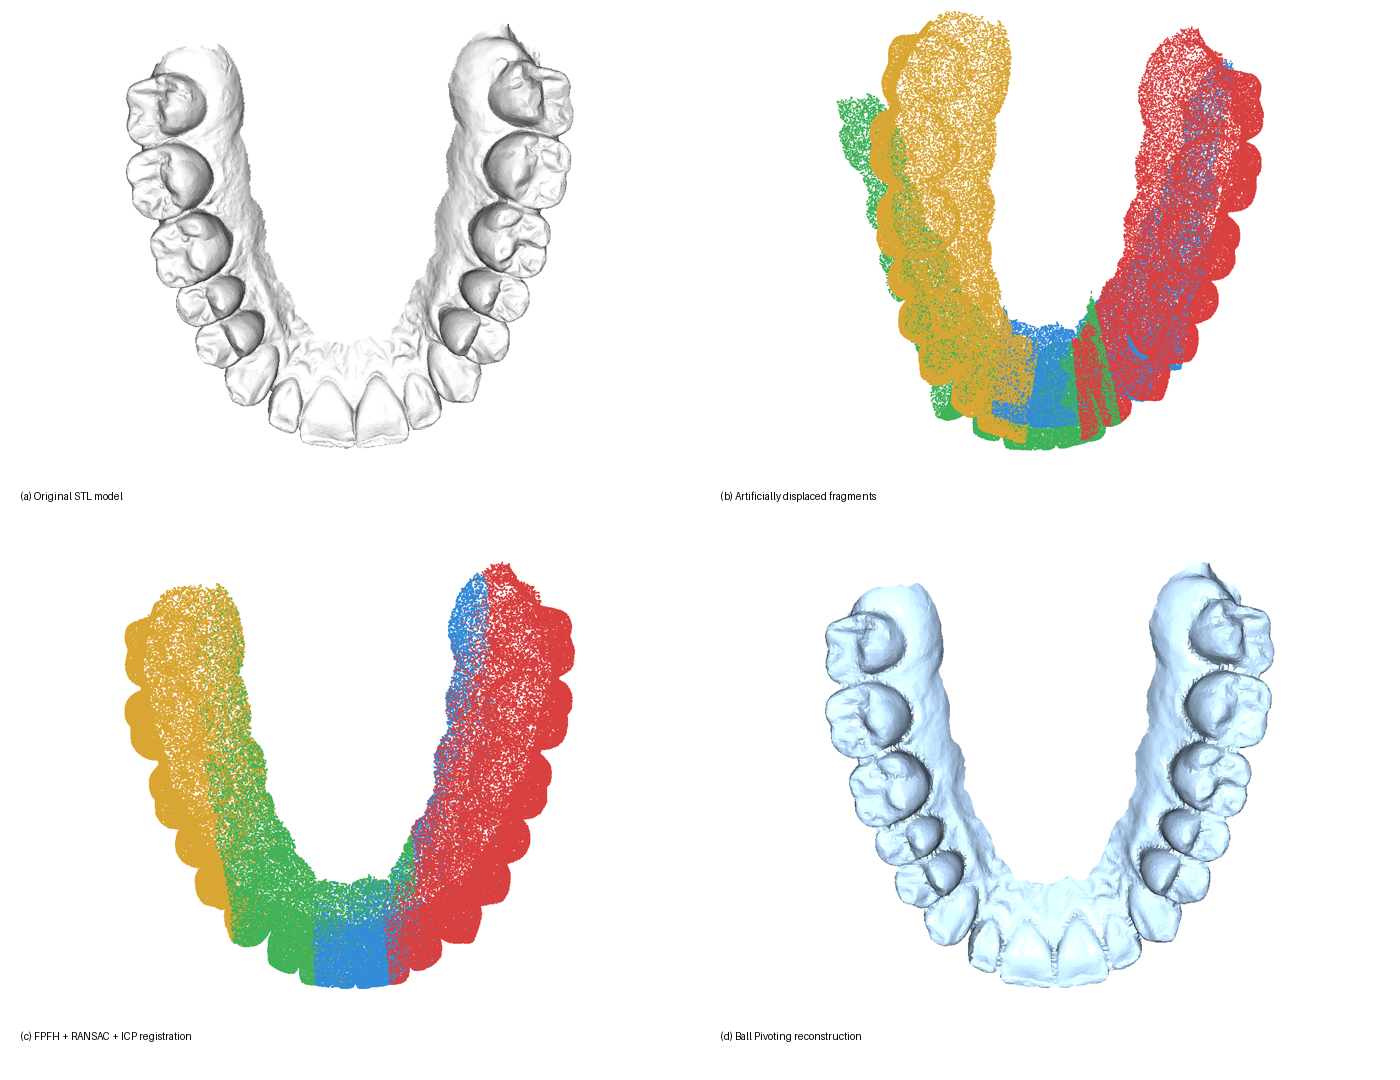
\includegraphics[width=0.96\textwidth]{assets/marvin/realistic_validation_workflow.png}
    \caption{Representative realistic-validation workflow using Model~1 upper jaw. The original STL surface is sampled, split into overlapping fragments, displaced by known rigid transformations, registered with FPFH + RANSAC + Point-to-Plane ICP, and reconstructed with Ball Pivoting. Quantitative evaluation was performed on ten jaw meshes.}
    \label{fig:realistic-validation-workflow}
\end{figure*}

\subsection{Registration Methods}
\label{sec:marvin-registration-methods}

A rigid transformation maps a source point $\mathbf{p}$ to a target point $\mathbf{p}'$ by
\begin{equation}
    \mathbf{p}' = R\mathbf{p} + \mathbf{t},
\end{equation}
where $R\in SO(3)$ is the rotation matrix and $\mathbf{t}\in\mathbb{R}^{3}$ is the translation vector. The implementation consistently uses the convention source $\rightarrow$ target. This convention is especially important when pairwise transformations are chained during multiway registration.

Five registration variants were implemented. Point-to-Point ICP and Point-to-Plane ICP follow the classical local ICP formulation \cite{kraus_besl1992,kraus_chen1992}. Generalized ICP (GICP) extends local matching by incorporating local covariance information \cite{kraus_segal2009}. The two global-to-local pipelines first compute Fast Point Feature Histogram (FPFH) descriptors \cite{kraus_rusu2009}, perform either RANSAC-based feature matching or FGR \cite{kraus_zhou2016}, and then refine the resulting transformation with Point-to-Plane ICP \cite{kraus_lyu2024}.

\begin{table}[!t]
\centering
\footnotesize
\setlength{\tabcolsep}{3pt}
\begin{tabularx}{\columnwidth}{@{}lYY@{}}
\toprule
\textbf{Method} & \textbf{Main advantage} & \textbf{Main limitation} \\
\midrule
Point-to-Point ICP & Simple and fast local refinement & Small capture range \\
Point-to-Plane ICP & Accurate local surface alignment & Requires normals and a good initial pose \\
Generalized ICP & Strong local surface adaptation & Still initialization dependent \\
FPFH + RANSAC + ICP & Large capture range and robust global hypotheses & Stochastic and slower \\
FPFH + FGR + ICP & Fast global initialization with ICP refinement & Sensitive to ambiguous feature correspondences \\
\bottomrule
\end{tabularx}
\caption{Implemented registration methods.}
\label{tab:registration-methods}
\end{table}

All algorithms share the same preprocessing wherever possible. Point clouds are voxel-downsampled with a voxel size of $0.5$, normals are estimated within a radius of $2.0$ voxel sizes using at most 30 neighbors, and FPFH descriptors use a radius of $5.0$ voxel sizes and at most 100 neighbors. RANSAC uses three correspondences per hypothesis, up to 100,000 iterations, and a confidence of $0.999$. The final local refinement uses Point-to-Plane ICP with a correspondence distance of $0.4$ voxel sizes. Open3D 0.19.0 provides the geometric processing and registration primitives \cite{kraus_open3d019}.

\begin{figure}[!t]
\centering
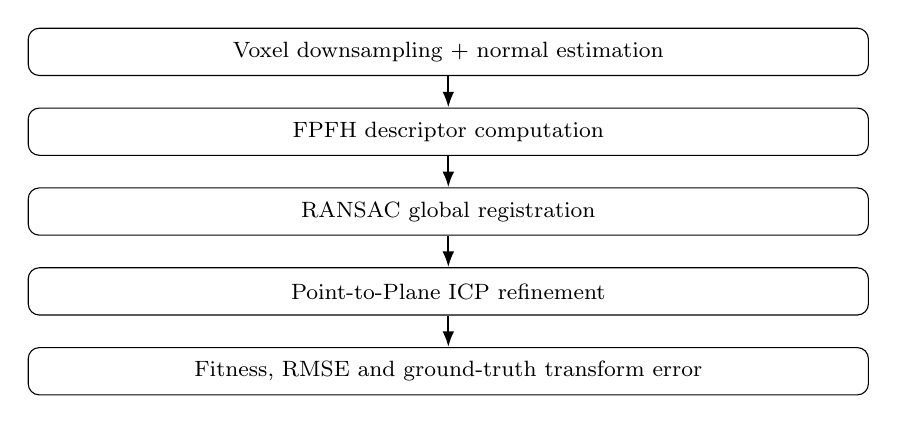
\begin{tikzpicture}[
    node distance=4mm,
    box/.style={draw, rounded corners, align=center, minimum width=0.88\columnwidth, minimum height=6mm, font=\footnotesize},
    arr/.style={-{Latex[length=2mm]}, thick}
]
\node[box] (pre) {Voxel downsampling + normal estimation};
\node[box, below=of pre] (fpfh) {FPFH descriptor computation};
\node[box, below=of fpfh] (ransac) {RANSAC global registration};
\node[box, below=of ransac] (icp) {Point-to-Plane ICP refinement};
\node[box, below=of icp] (eval) {Fitness, RMSE and ground-truth transform error};
\draw[arr] (pre) -- (fpfh);
\draw[arr] (fpfh) -- (ransac);
\draw[arr] (ransac) -- (icp);
\draw[arr] (icp) -- (eval);
\end{tikzpicture}
\caption{Final pairwise registration pipeline after realistic validation.}
\label{fig:final-ransac-pipeline}
\end{figure}

\subsection{Implementation Structure and Evaluation Metrics}
\label{sec:marvin-implementation-metrics}

The implementation uses a small modular Python/Open3D architecture so that preprocessing, algorithms, evaluation, visualization, and mesh construction can be exchanged independently. The registration layer contains the five pairwise methods behind a common result interface, while the reconstruction layer contains Poisson/BPA reconstruction, cleanup, topology analysis, simplification, and export. This separation was important for the experimental workflow because the same preprocessing and evaluation code could be reused for synthetic and realistic datasets.

\begin{table}[!t]
\centering
\footnotesize
\setlength{\tabcolsep}{3pt}
\begin{tabularx}{\columnwidth}{@{}lY@{}}
\toprule
\textbf{Component} & \textbf{Responsibility} \\
\midrule
Preprocessing & Voxel downsampling, normal estimation, FPFH descriptors \\
Registration algorithms & P2P ICP, P2Plane ICP, GICP, FPFH+RANSAC+ICP, FPFH+FGR+ICP \\
Evaluation & Fitness, inlier RMSE, translation/rotation ground-truth error \\
Multiway registration & Pairwise chaining, pose evaluation, merged cloud export \\
Mesh reconstruction & Poisson and Ball Pivoting \\
Mesh analysis & Components, manifold tests, self-intersections, bidirectional distances \\
Mesh export & Simplification, cleanup, PLY/STL serialization and reload test \\
\bottomrule
\end{tabularx}
\caption{Functional structure of the implemented registration and model-construction pipeline.}
\label{tab:software-structure}
\end{table}

\paragraph{Software architecture.}
The code base separates the importable implementation under \texttt{src/registration3d} from experiment drivers, diagnostic scripts, and report-visualization utilities. Within the core package, registration algorithms follow a strategy-style interface: Point-to-Point ICP, Point-to-Plane ICP, GICP, FPFH+RANSAC+ICP, and FPFH+FGR+ICP expose the same \texttt{register(...)} operation and return a standardized result object. This allows the same evaluator and benchmark logic to be reused without algorithm-specific branches. The two feature-based methods additionally share the same FPFH extractor. Multiway registration accepts an interchangeable pairwise registration strategy and produces a merged point cloud, which is deliberately treated as the boundary between registration and surface reconstruction. The mesh stage is similarly separated into reconstruction, cleanup, topology/distance evaluation, simplification, and export.

\begin{samepage}
When ground truth is available, translation error is computed as
\begin{equation}
    e_t = \lVert \mathbf{t}_{est} - \mathbf{t}_{GT} \rVert_2,
\end{equation}
and rotation error as
\begin{equation}
    e_R = \cos^{-1}\left(\frac{\mathrm{tr}(R_{est}R_{GT}^{T})-1}{2}\right).
\end{equation}
\end{samepage}
The realistic robustness study classifies a result as successful when $e_t\leq1$ model unit and $e_R\leq1^\circ$. This explicit transform-based criterion avoids the ambiguity of relying only on fitness or inlier RMSE.

\subsection{Synthetic Registration Evaluation}
\label{sec:marvin-synthetic-registration}

\subsubsection{Evaluation Setup}

Synthetic dental-like source and target clouds were generated with known rigid ground truth. Four disturbance variables were varied independently: overlap, rotation, translation, and additive positional noise. Each condition was evaluated in 10 reproducible repetitions. Within a given stress-test series, the same repetition index uses the same dataset seed across all values of the varied parameter, while stochastic registration methods receive reproducible algorithm seeds. This design reduces unintended variation between neighboring conditions and allows direct evaluation of the estimated transformation rather than relying only on correspondence-based metrics.

\begin{table}[H]
\centering
\footnotesize
\begin{tabularx}{\columnwidth}{@{}lY@{}}
\toprule
\textbf{Experiment} & \textbf{Tested values} \\
\midrule
Overlap & 0.20, 0.30, 0.40, 0.50, 0.60, 0.70, 0.80 \\
Rotation & $0^\circ$, $5^\circ$, $10^\circ$, $20^\circ$, $30^\circ$, $40^\circ$, $60^\circ$ \\
Translation & 0, 1, 2, 4, 6, 8, 12 \\
Noise standard deviation & 0, 0.01, 0.025, 0.05, 0.10, 0.20 \\
\bottomrule
\end{tabularx}
\caption{Controlled synthetic registration experiments. Each parameter value was evaluated with $n=10$ reproducible repetitions.}
\label{tab:synthetic-registration-setup}
\end{table}

The principal metrics were fitness, inlier RMSE, translation error, rotation error, runtime, and success rate. Fitness and inlier RMSE alone were not treated as correctness guarantees: repetitive dental geometry can produce geometrically plausible but semantically incorrect correspondences. Whenever ground truth was available, translation and rotation errors were therefore decisive.

\begin{figure*}[!t]
\centering
\begin{subfigure}[t]{0.48\textwidth}
    \centering
    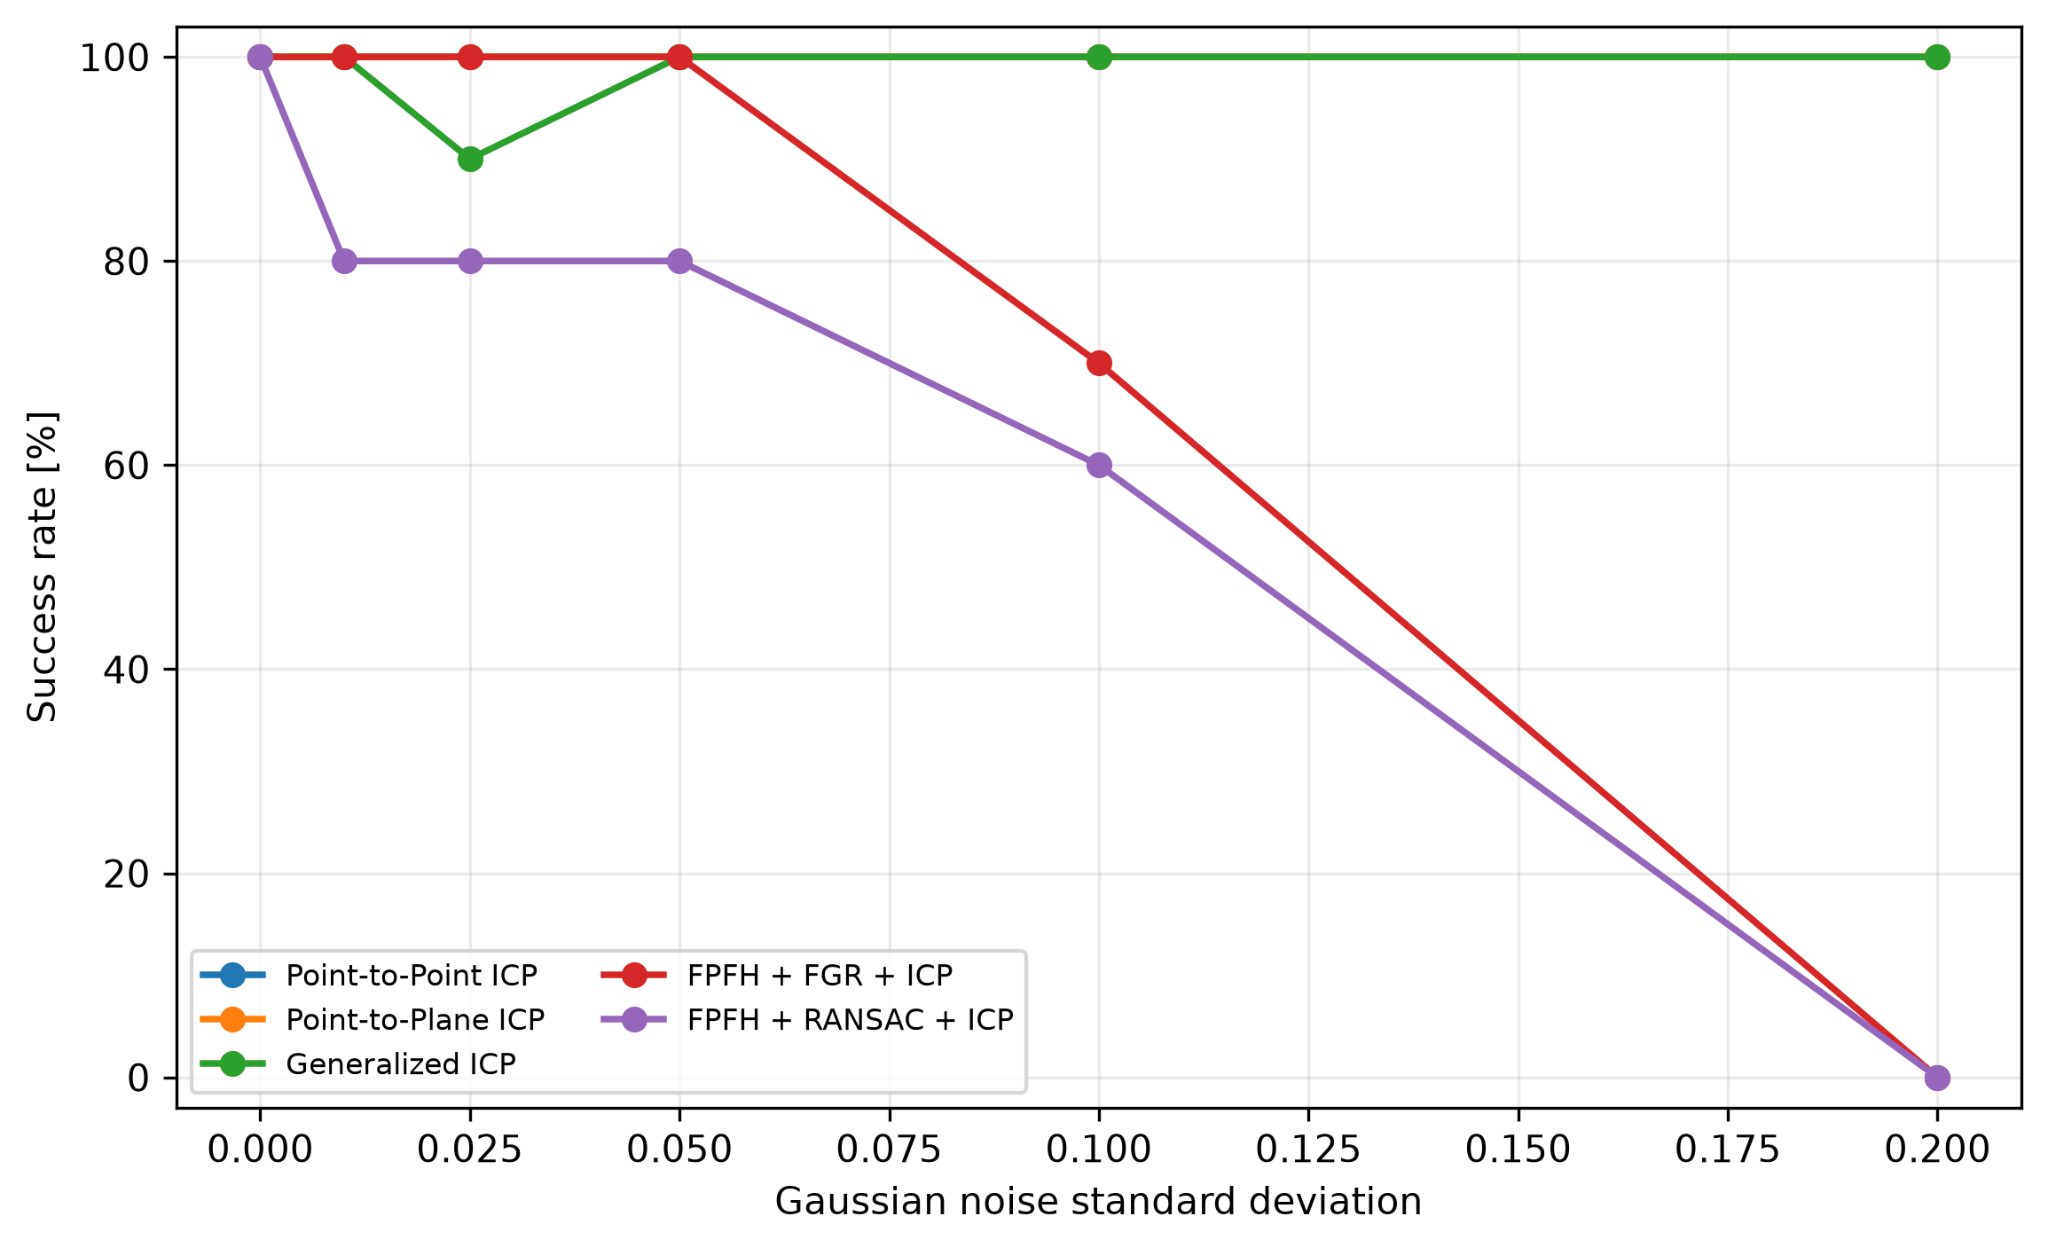
\includegraphics[width=\linewidth]{assets/marvin/noise_success_rate.png}
    \caption{Noise.}
\end{subfigure}
\hfill
\begin{subfigure}[t]{0.48\textwidth}
    \centering
    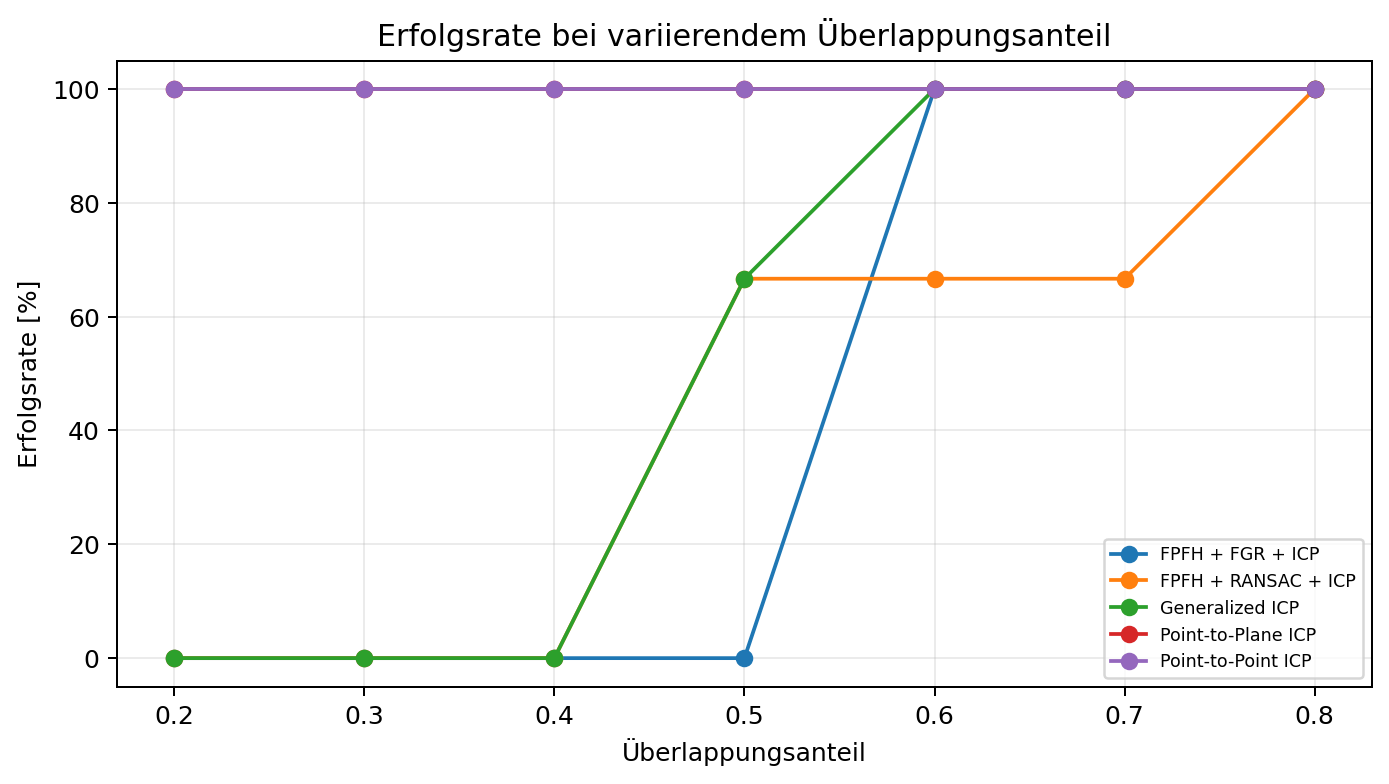
\includegraphics[width=\linewidth]{assets/marvin/overlap_success_rate.png}
    \caption{Overlap.}
\end{subfigure}

\vspace{2mm}

\begin{subfigure}[t]{0.48\textwidth}
    \centering
    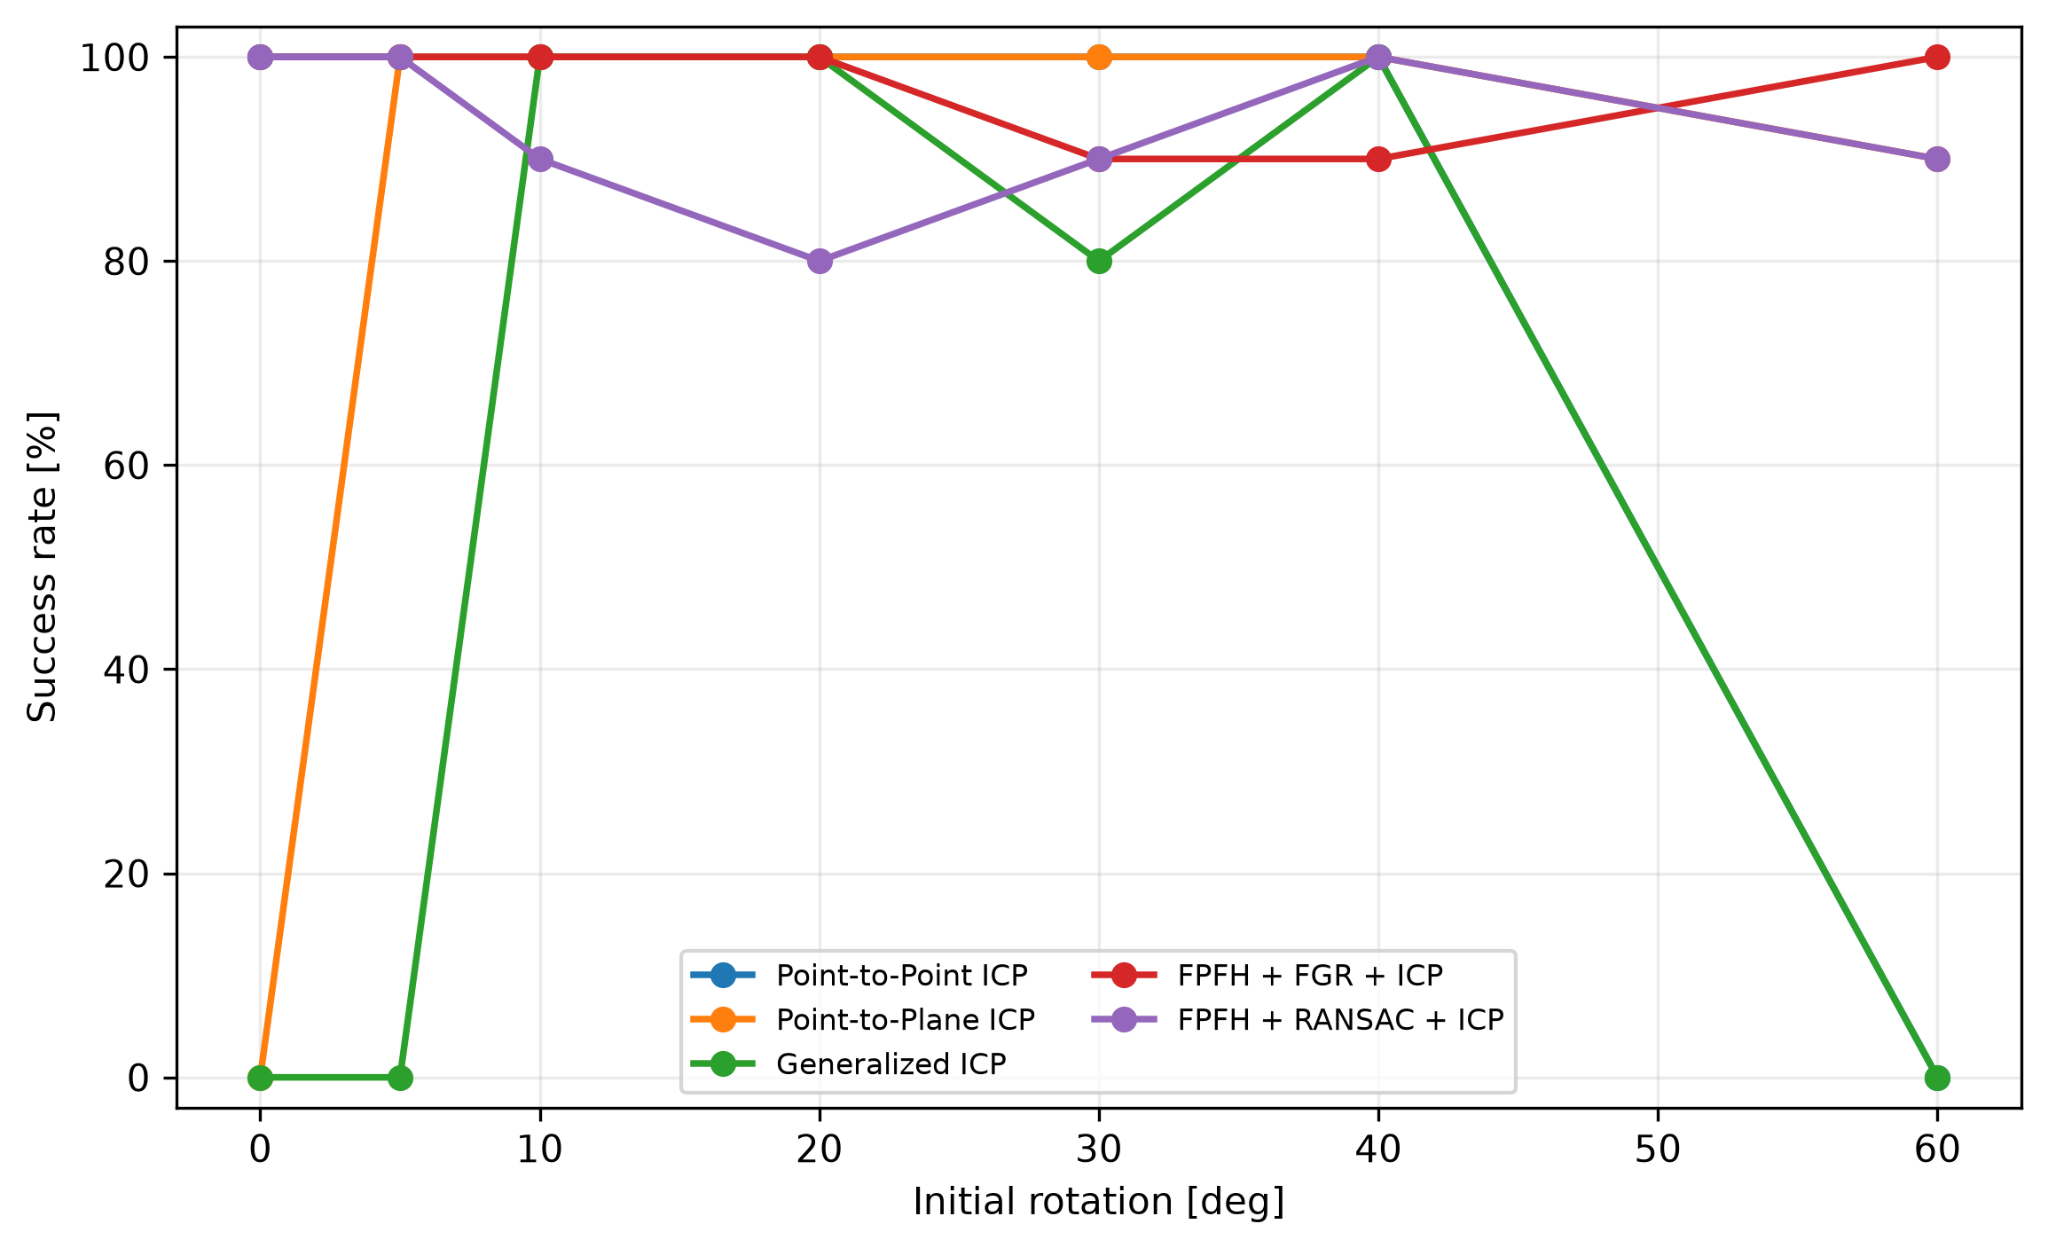
\includegraphics[width=\linewidth]{assets/marvin/rotation_success_rate.png}
    \caption{Rotation.}
\end{subfigure}
\hfill
\begin{subfigure}[t]{0.48\textwidth}
    \centering
    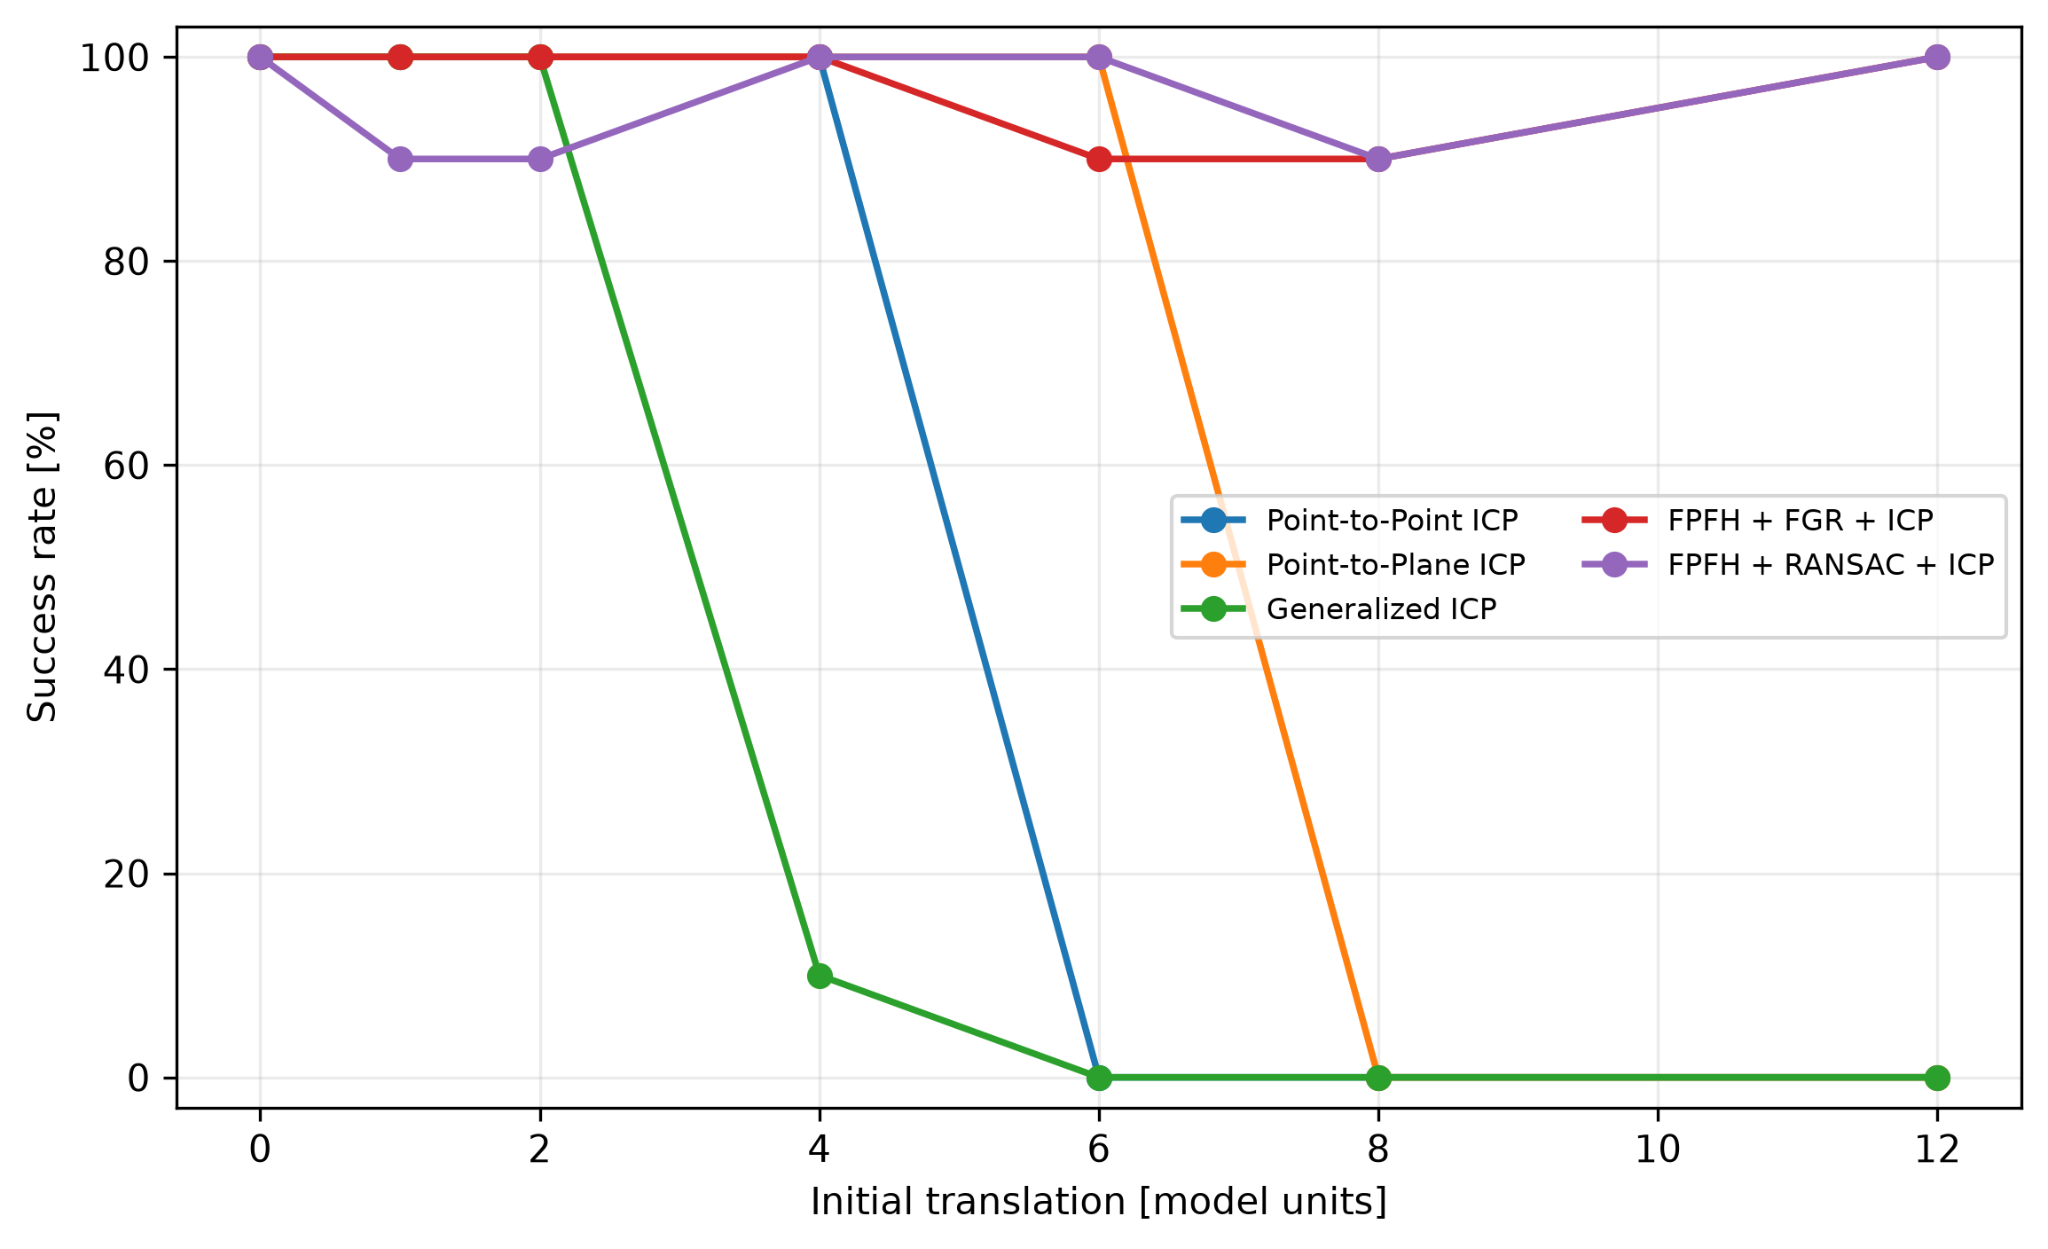
\includegraphics[width=\linewidth]{assets/marvin/translation_success_rate.png}
    \caption{Translation.}
\end{subfigure}
\caption{Success-rate curves from the controlled synthetic pairwise experiments ($n=10$ repetitions per parameter value). The curves should be interpreted as empirical behavior on the specific dental-like geometry rather than as universal monotonic capture-range characteristics.}
\label{fig:synthetic-success-rates}
\end{figure*}

\begin{table*}[!t]
\centering
\footnotesize
\setlength{\tabcolsep}{4pt}
\begin{tabularx}{\textwidth}{@{}lYYYYY@{}}
\toprule
\textbf{Stress case} & \textbf{P2P ICP} & \textbf{P2Plane ICP} & \textbf{GICP} & \textbf{RANSAC + ICP} & \textbf{FGR + ICP} \\
\midrule
Favorable initialization & Very strong & Very strong & Very strong & Strong & Strong \\
Large translation & Capture-range failures & Capture-range failures & Capture-range failures & Robust global recovery & Robust global recovery \\
Low overlap & Can converge locally if initialized well & Can converge locally if initialized well & Can remain locally accurate & Ambiguous feature matches & Ambiguous feature matches \\
High rotation & Fails at the largest tested angle & Non-monotonic local-minimum behavior & Strongly non-monotonic & Large capture range & Large capture range \\
Strong synthetic noise & Stable only with favorable initialization & Stable only with favorable initialization & Stable only with favorable initialization & Global feature matching degraded & Global feature matching degraded \\
\bottomrule
\end{tabularx}
\caption{Qualitative behavior observed in the controlled synthetic stress tests. The table summarizes failure modes rather than claiming a universal algorithm ranking.}
\label{tab:synthetic-behavior-summary}
\end{table*}

\paragraph{Interpretation of overlap and rotation.}
The updated 10-repeat overlap study removes an apparent non-monotonicity that was present in an earlier exploratory plot. For FPFH + RANSAC + ICP, the observed success rates increase from 0\% at overlaps 0.20--0.40 to 40\% at 0.50, 90\% at 0.60 and 0.70, and 100\% at 0.80. FGR shows an even sharper transition, remaining at 0\% through 0.50 and reaching 100\% from 0.60 onward. This supports the interpretation that, on the synthetic dental-like geometry, the feature-based methods require a sufficiently large common visible region before FPFH correspondences become reliably distinctive.

The rotation series exhibits a notable non-monotonic behavior for Point-to-Plane ICP. An input rotation of $0^\circ$ does not correspond to a perfectly aligned pair: the series keeps overlap at 0.60, translation magnitude at 3 model units, and Gaussian noise at $\sigma=0.02$. Under this translation-only displacement, Point-to-Plane ICP converged consistently to an incorrect local solution, with mean translation error 3.5399 model units and mean rotation error $7.336^\circ$. For rotations from $5^\circ$ through $40^\circ$, the altered correspondence configuration instead led to a favorable convergence basin, producing 100\% success and mean translation errors of approximately 0.017--0.021 model units. At $60^\circ$, one of ten runs failed, reducing success to 90\%. This result is interpreted as a dataset-specific local-minimum effect: it does not imply that adding rotation generally improves ICP, but rather that the correspondence landscape of the repetitive synthetic geometry changes with the applied pose.


GICP shows a similarly non-monotonic rotation response, although for a slightly different reason. It is still a local iterative method and therefore remains sensitive to the nearest-neighbor correspondences induced by the initial pose. In addition, its residual is weighted by local covariance information, so a change in relative orientation alters both the correspondences and the covariance-weighted objective. On the repetitive synthetic dental-like geometry, different input rotations can therefore move the optimizer between substantially different convergence basins. The observed fluctuations are interpreted as correspondence and local-minimum effects of this particular dataset, not as a monotonic relationship between larger rotations and better or worse GICP performance.

\subsubsection{Synthetic Findings and Provisional Selection}

The synthetic experiments highlighted the expected trade-off. Local ICP variants were fast and highly accurate whenever the initial alignment remained inside their capture range, but they failed for larger displacements. Feature-based global registration handled larger initial pose differences but was more sensitive to low overlap, repetitive geometry, and noise.

Under the original synthetic benchmark, FPFH + FGR + Point-to-Plane ICP provided the most attractive overall compromise between global capture range, precision after local refinement, and runtime. It was therefore selected \emph{provisionally} for the first multiway baseline. This was not treated as a universal ranking; the later realistic validation was explicitly intended to challenge this choice.

A four-fragment synthetic multiway test confirmed that FGR + ICP could produce a precise chain under the controlled test conditions. The maximum node translation error was approximately $0.0047$ and the maximum rotation error approximately $0.035^\circ$, while the merged cloud contained 22,022 points. Additional multi-start and cycle-consistency experiments showed, however, that high fitness can still occur for incorrect dental alignments. This observation motivated the second validation stage on realistic jaw geometry.

\subsubsection{Synthetic Multiway Baseline and Robustness Analysis}

The synthetic multiway dataset contains four partially overlapping fragments with 13,793, 15,302, 16,193, and 15,069 points. The controlled acquisition model again follows $\mathbf{x}_i=A_i\mathbf{x}_{world}$, so the exact pose of fragment $i$ in the global reference frame is $A_i^{-1}$. For the provisional FGR baseline, only sequential odometry edges were used. Loop closures were deliberately disabled to measure the selected pairwise method without global correction.

\begin{figure}[!t]
\centering
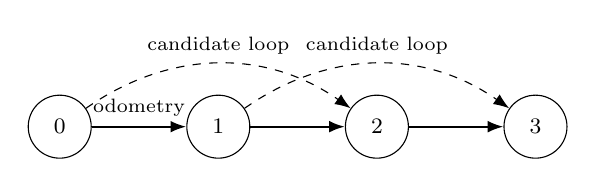
\begin{tikzpicture}[
  node distance=12mm,
  frag/.style={circle,draw,minimum size=8mm,font=\footnotesize},
  odo/.style={-{Latex[length=2mm]},thick},
  loop/.style={-{Latex[length=2mm]},dashed}
]
\node[frag] (f0) {0};
\node[frag, right=of f0] (f1) {1};
\node[frag, right=of f1] (f2) {2};
\node[frag, right=of f2] (f3) {3};
\draw[odo] (f0) -- node[above,font=\scriptsize]{odometry} (f1);
\draw[odo] (f1) -- (f2);
\draw[odo] (f2) -- (f3);
\draw[loop,bend left=35] (f0) to node[above,font=\scriptsize]{candidate loop} (f2);
\draw[loop,bend left=35] (f1) to node[above,font=\scriptsize]{candidate loop} (f3);
\end{tikzpicture}
\caption{Synthetic four-fragment pose-graph concept. Solid edges form the evaluated sequential baseline; dashed loop candidates were examined only in the optional robustness analysis.}
\label{fig:synthetic-pose-graph}
\end{figure}

\begin{table}[H]
\centering
\footnotesize
\begin{tabular}{lrr}
\toprule
\textbf{Odometry edge} & \textbf{Fitness} & \textbf{Inlier RMSE} \\
\midrule
$0\rightarrow1$ & 0.7397 & 0.2499 \\
$1\rightarrow2$ & 0.6904 & 0.2493 \\
$2\rightarrow3$ & 0.6676 & 0.2466 \\
\bottomrule
\end{tabular}
\caption{Synthetic four-fragment FGR + ICP multiway baseline.}
\label{tab:synthetic-multiway-edges}
\end{table}

The resulting pose errors were 0 for fragment 0, 0.00424 / $0.00636^\circ$ for fragment 1, 0.00468 / $0.03513^\circ$ for fragment 2, and 0.00268 / $0.02626^\circ$ for fragment 3. The merged point cloud contained 22,022 points. Thus, under controlled synthetic conditions, sequential accumulation remained small.

A separate robustness analysis generated 20 FGR and 20 RANSAC hypotheses with deterministic seeds, clustered similar transformations, and ranked clusters by median RMSE. Candidate loop closures were also checked for cycle consistency. This procedure could recover correct odometry in ambiguous synthetic cases, but it was intentionally kept separate from the baseline algorithm comparison: cycle consistency can reject some inconsistent hypotheses, yet it cannot prove that a globally self-consistent chain is geometrically correct. The realistic validation therefore remained necessary.

\subsection{Validation on Realistic Dental Geometry}
\label{sec:marvin-realistic-registration}

\subsubsection{Five-Model Dataset Construction}

The realistic validation was expanded to five distinct dental model sets, each containing an upper- and lower-jaw STL mesh. The ten meshes have bounding-box diagonals between 79.696 and 92.084 model units; the ratio between the largest and smallest diagonal is only 1.155, so the same registration parameters can be used without rescaling. Every jaw surface was uniformly sampled to 120,000 points and split into four partially overlapping fragments along the first PCA axis with a nominal overlap of 60\%.

Known rigid acquisition transformations were applied using
\begin{equation}
    \mathbf{x}_i = A_i \mathbf{x}_{\mathrm{world}},
\end{equation}
so that the exact pairwise ground-truth transformation is
\begin{equation}
    T_{i\rightarrow j}^{GT} = A_j A_i^{-1}.
\end{equation}
The STL format itself does not encode physical units. All distances are therefore reported in model units.

\begin{table}[H]
\centering
\footnotesize
\begin{tabularx}{\columnwidth}{@{}lY@{}}
\toprule
\textbf{Property} & \textbf{Five-model validation suite} \\
\midrule
Dental model sets & 5 \\
Jaw meshes & 10 (5 upper, 5 lower) \\
Surface samples per jaw & 120,000 \\
Fragments per jaw & 4 \\
Adjacent pairwise cases & 30 \\
Nominal fragment overlap & 60\% \\
Bounding-box diagonal range & 79.696--92.084 model units \\
\bottomrule
\end{tabularx}
\caption{Realistic five-model validation dataset.}
\label{tab:realistic-dataset}
\end{table}


\begin{figure*}[!t]
\centering
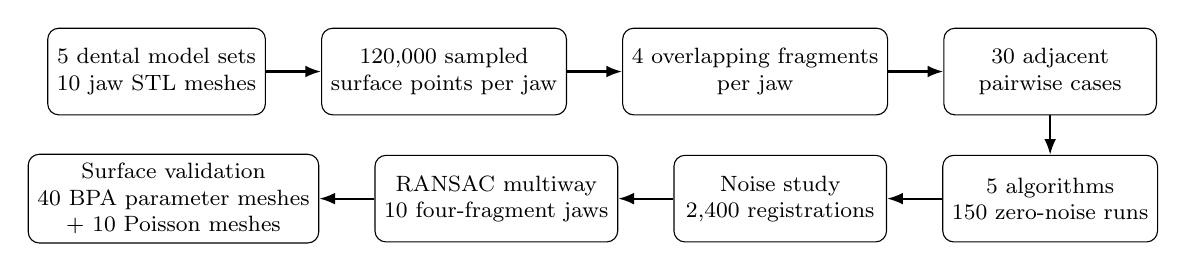
\begin{tikzpicture}[
    node distance=5mm and 7mm,
    box/.style={draw,rounded corners,align=center,minimum width=27mm,minimum height=11mm,font=\footnotesize},
    arr/.style={-{Latex[length=2mm]},thick}
]
\node[box] (stl) {5 dental model sets\\10 jaw STL meshes};
\node[box, right=of stl] (sample) {120,000 sampled\\surface points per jaw};
\node[box, right=of sample] (frag) {4 overlapping fragments\\per jaw};
\node[box, right=of frag] (pairs) {30 adjacent\\pairwise cases};
\node[box, below=of pairs] (pairbench) {5 algorithms\\150 zero-noise runs};
\node[box, left=of pairbench] (noise) {Noise study\\2,400 registrations};
\node[box, left=of noise] (multi) {RANSAC multiway\\10 four-fragment jaws};
\node[box, left=of multi] (mesh) {Surface validation\\40 BPA parameter meshes\\+ 10 Poisson meshes};
\draw[arr] (stl) -- (sample);
\draw[arr] (sample) -- (frag);
\draw[arr] (frag) -- (pairs);
\draw[arr] (pairs) -- (pairbench);
\draw[arr] (pairbench) -- (noise);
\draw[arr] (noise) -- (multi);
\draw[arr] (multi) -- (mesh);
\end{tikzpicture}
\caption{Five-model evaluation protocol. The same ten jaw geometries are propagated from controlled virtual fragmentation through pairwise comparison, noise robustness, sequential multiway registration, and surface-reconstruction validation.}
\label{fig:model-suite-protocol}
\end{figure*}

The experimental protocol deliberately separates geometric diversity from stochastic repetition. The zero-noise benchmark contains 30 distinct adjacent fragment pairs, while the nonzero-noise conditions repeat these same base pairs with three independently seeded perturbations. This distinction prevents repeated perturbations from being presented as additional independent dental geometries. The same fragmented jaws are then reused for the RANSAC multiway experiment and for surface reconstruction, so registration and mesh quality can be evaluated along one consistent end-to-end path.


\begin{figure}[!t]
    \centering
    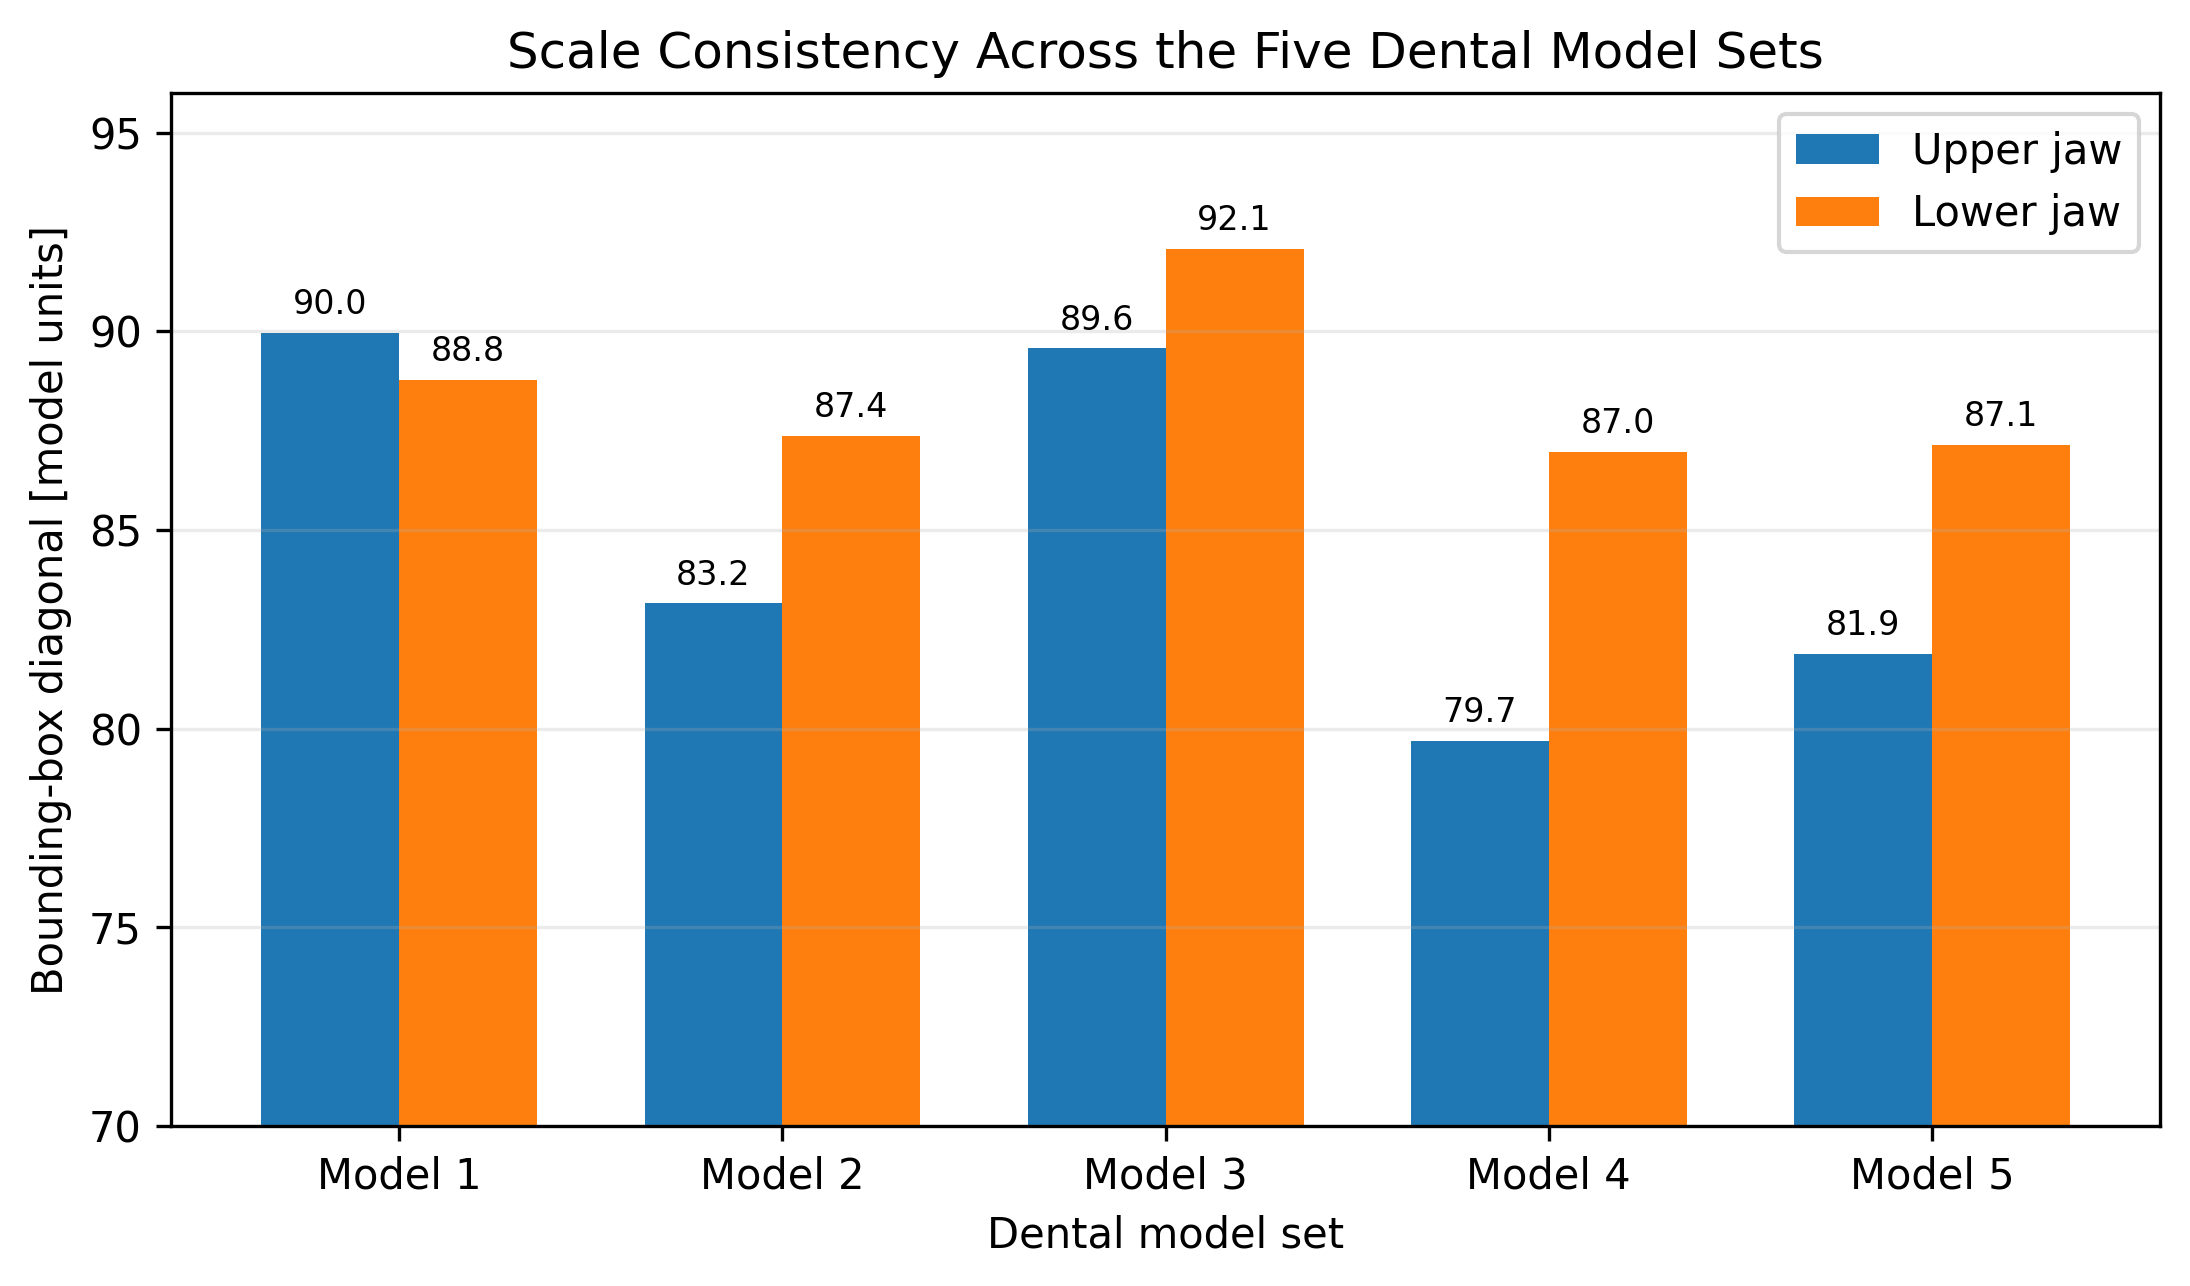
\includegraphics[width=\columnwidth]{assets/marvin/model_suite/model_suite_scale_distribution.png}
    \caption{Bounding-box diagonal for all ten realistic jaw meshes. The relatively narrow range (79.696--92.084 model units) supports using one common registration parameterization, while also showing that the validation does not intentionally span extreme anatomical scale differences.}
    \label{fig:model-suite-scale}
\end{figure}

\begin{figure*}[!t]
\centering
\begin{subfigure}[t]{0.32\textwidth}
    \centering
    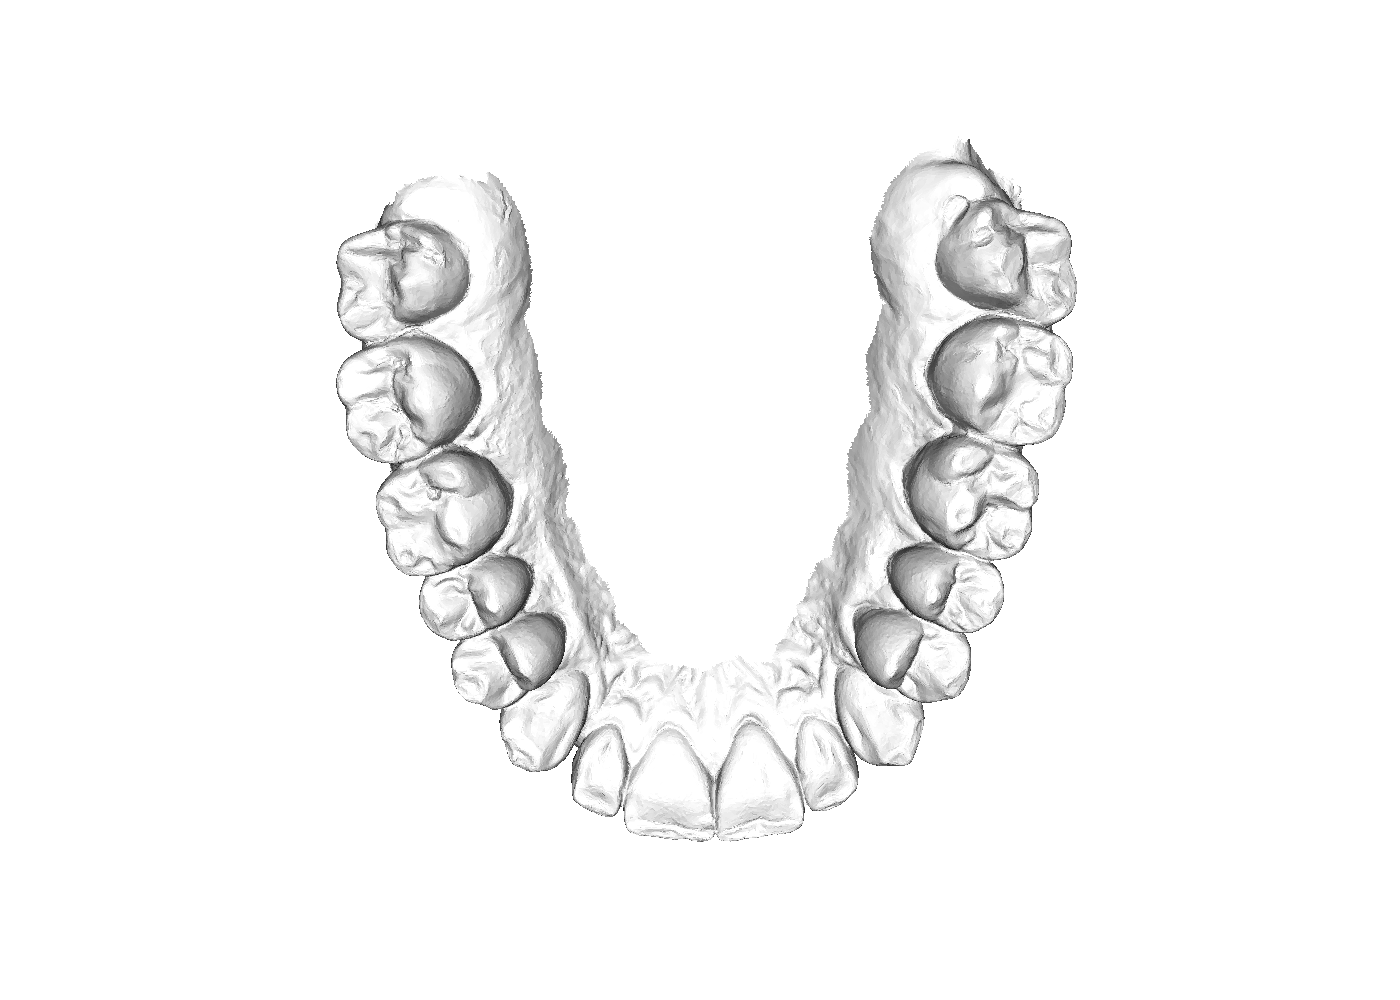
\includegraphics[width=\linewidth]{assets/marvin/upper_original.png}
    \caption{Model~1 upper-jaw STL.}
\end{subfigure}\hfill
\begin{subfigure}[t]{0.32\textwidth}
    \centering
    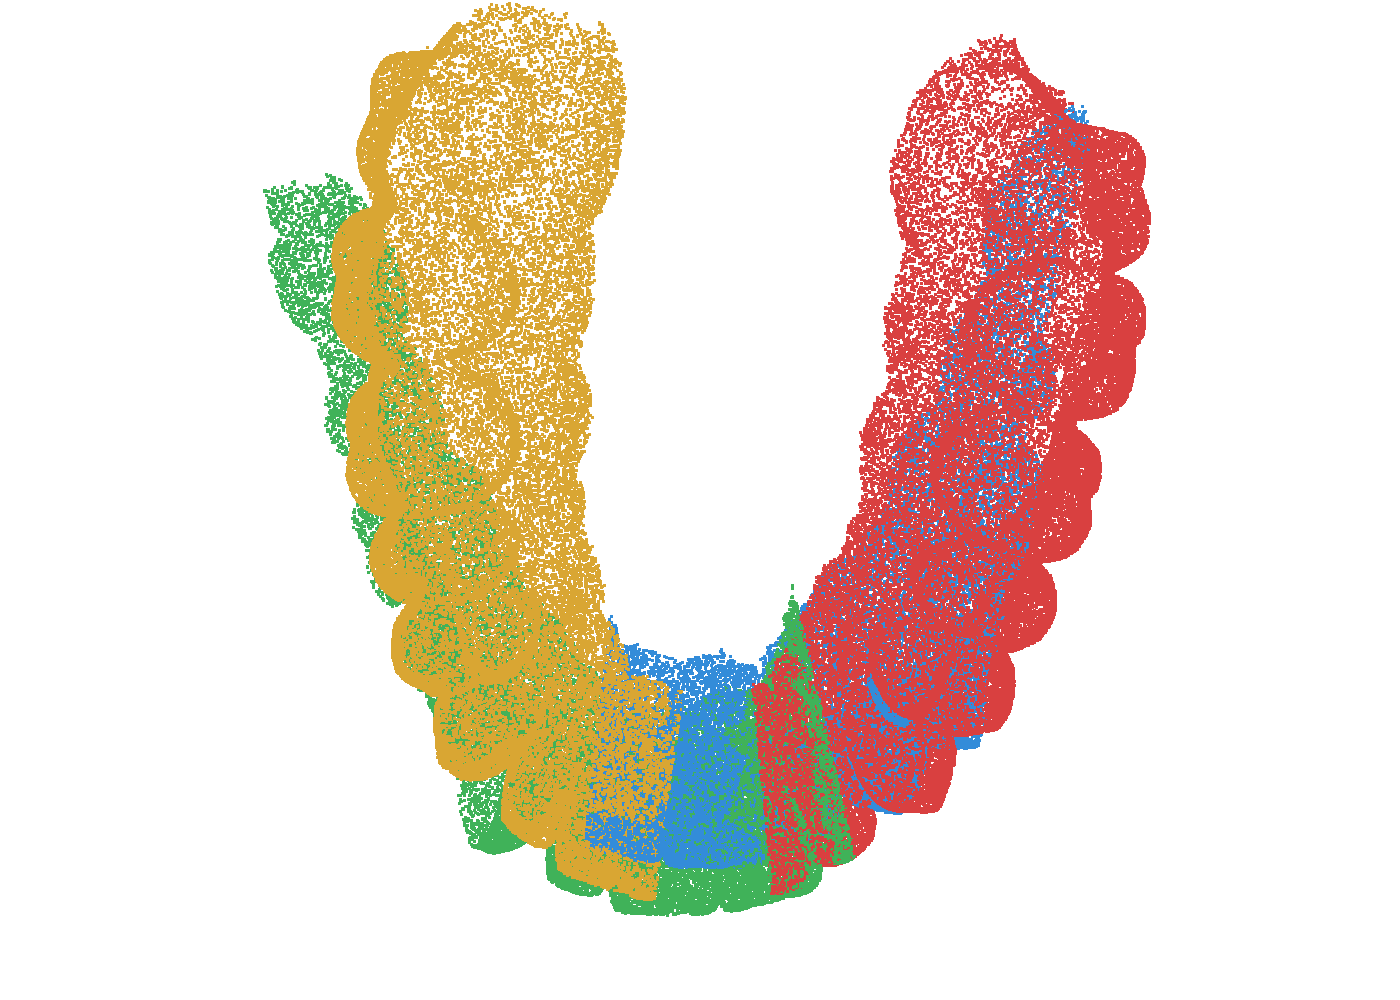
\includegraphics[width=\linewidth]{assets/marvin/upper_displaced.png}
    \caption{Displaced fragments.}
\end{subfigure}\hfill
\begin{subfigure}[t]{0.32\textwidth}
    \centering
    
\includegraphics[width=\linewidth]{assets/marvin/upper_registered.png}
    \caption{Registered fragments.}
\end{subfigure}
\caption{Representative qualitative example from Model~1. The quantitative registration experiments use all five model sets and all ten jaw meshes.}
\label{fig:realistic-representative-registration}
\end{figure*}

\subsubsection{Pairwise Comparison Across 30 Fragment Pairs}

The same five registration algorithms and preprocessing parameters were applied to the adjacent fragment pairs $0\rightarrow1$, $1\rightarrow2$, and $2\rightarrow3$ for every jaw. This yields 30 geometrically distinct zero-noise pairwise cases. Success requires translation error $\leq1$ model unit and rotation error $\leq1^\circ$.

\begin{table*}[!t]
\centering
\footnotesize
\setlength{\tabcolsep}{4pt}
\begin{tabular}{lrrrrrr}
\toprule
\textbf{Method} & \textbf{Success} & \textbf{Mean $e_t$} & \textbf{Median $e_t$} & \textbf{Mean $e_R$ [$^\circ$]} & \textbf{Median $e_R$ [$^\circ$]} & \textbf{Runtime [s]} \\
\midrule
Point-to-Point ICP & 50.0\% & 2.395165 & 0.226672 & 8.768677 & 0.899657 & 0.283623 \\
Point-to-Plane ICP & 80.0\% & 1.842892 & 0.013040 & 6.905271 & 0.070498 & 0.131327 \\
Generalized ICP & 73.3\% & 1.632389 & 0.001382 & 8.141821 & 0.008669 & 0.141021 \\
FPFH + FGR + ICP & 73.3\% & 3.977360 & 0.001573 & 10.316597 & 0.010267 & 0.891728 \\
\textbf{FPFH + RANSAC + ICP} & \textbf{100.0\%} & \textbf{0.001921} & \textbf{0.001509} & \textbf{0.009483} & \textbf{0.009741} & 0.681506 \\
\bottomrule
\end{tabular}
\caption{Pairwise registration summary across 30 adjacent fragment pairs from ten jaw meshes. Large mean-to-median gaps for several competing methods are caused by catastrophic registration failures.}
\label{tab:realistic-pairwise-summary}
\end{table*}

\begin{figure*}[!t]
\centering
\begin{subfigure}[t]{0.48\textwidth}
    \centering
    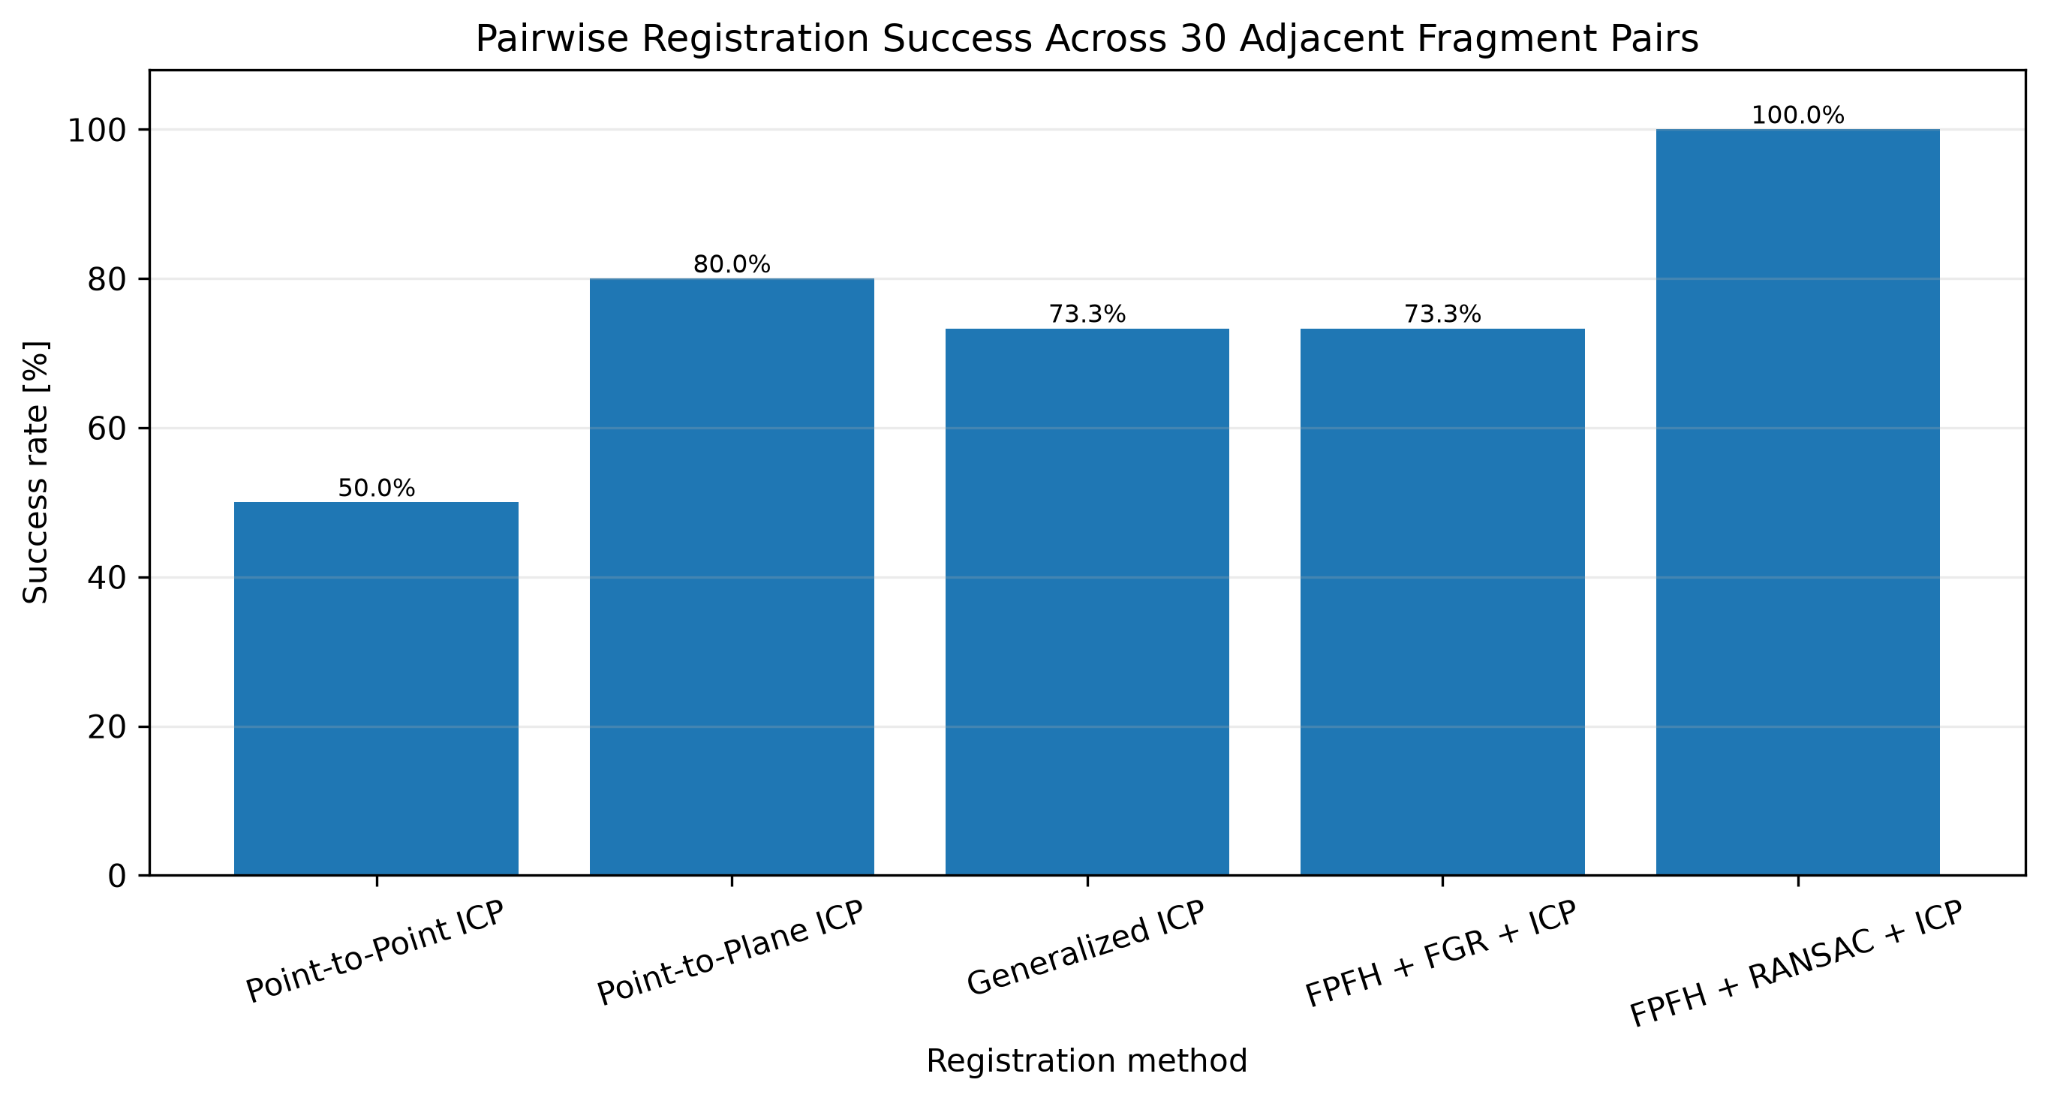
\includegraphics[width=\linewidth]{assets/marvin/model_suite/model_suite_pairwise_success_rate.png}
    \caption{Overall success across 30 cases.}
\end{subfigure}\hfill
\begin{subfigure}[t]{0.48\textwidth}
    \centering
    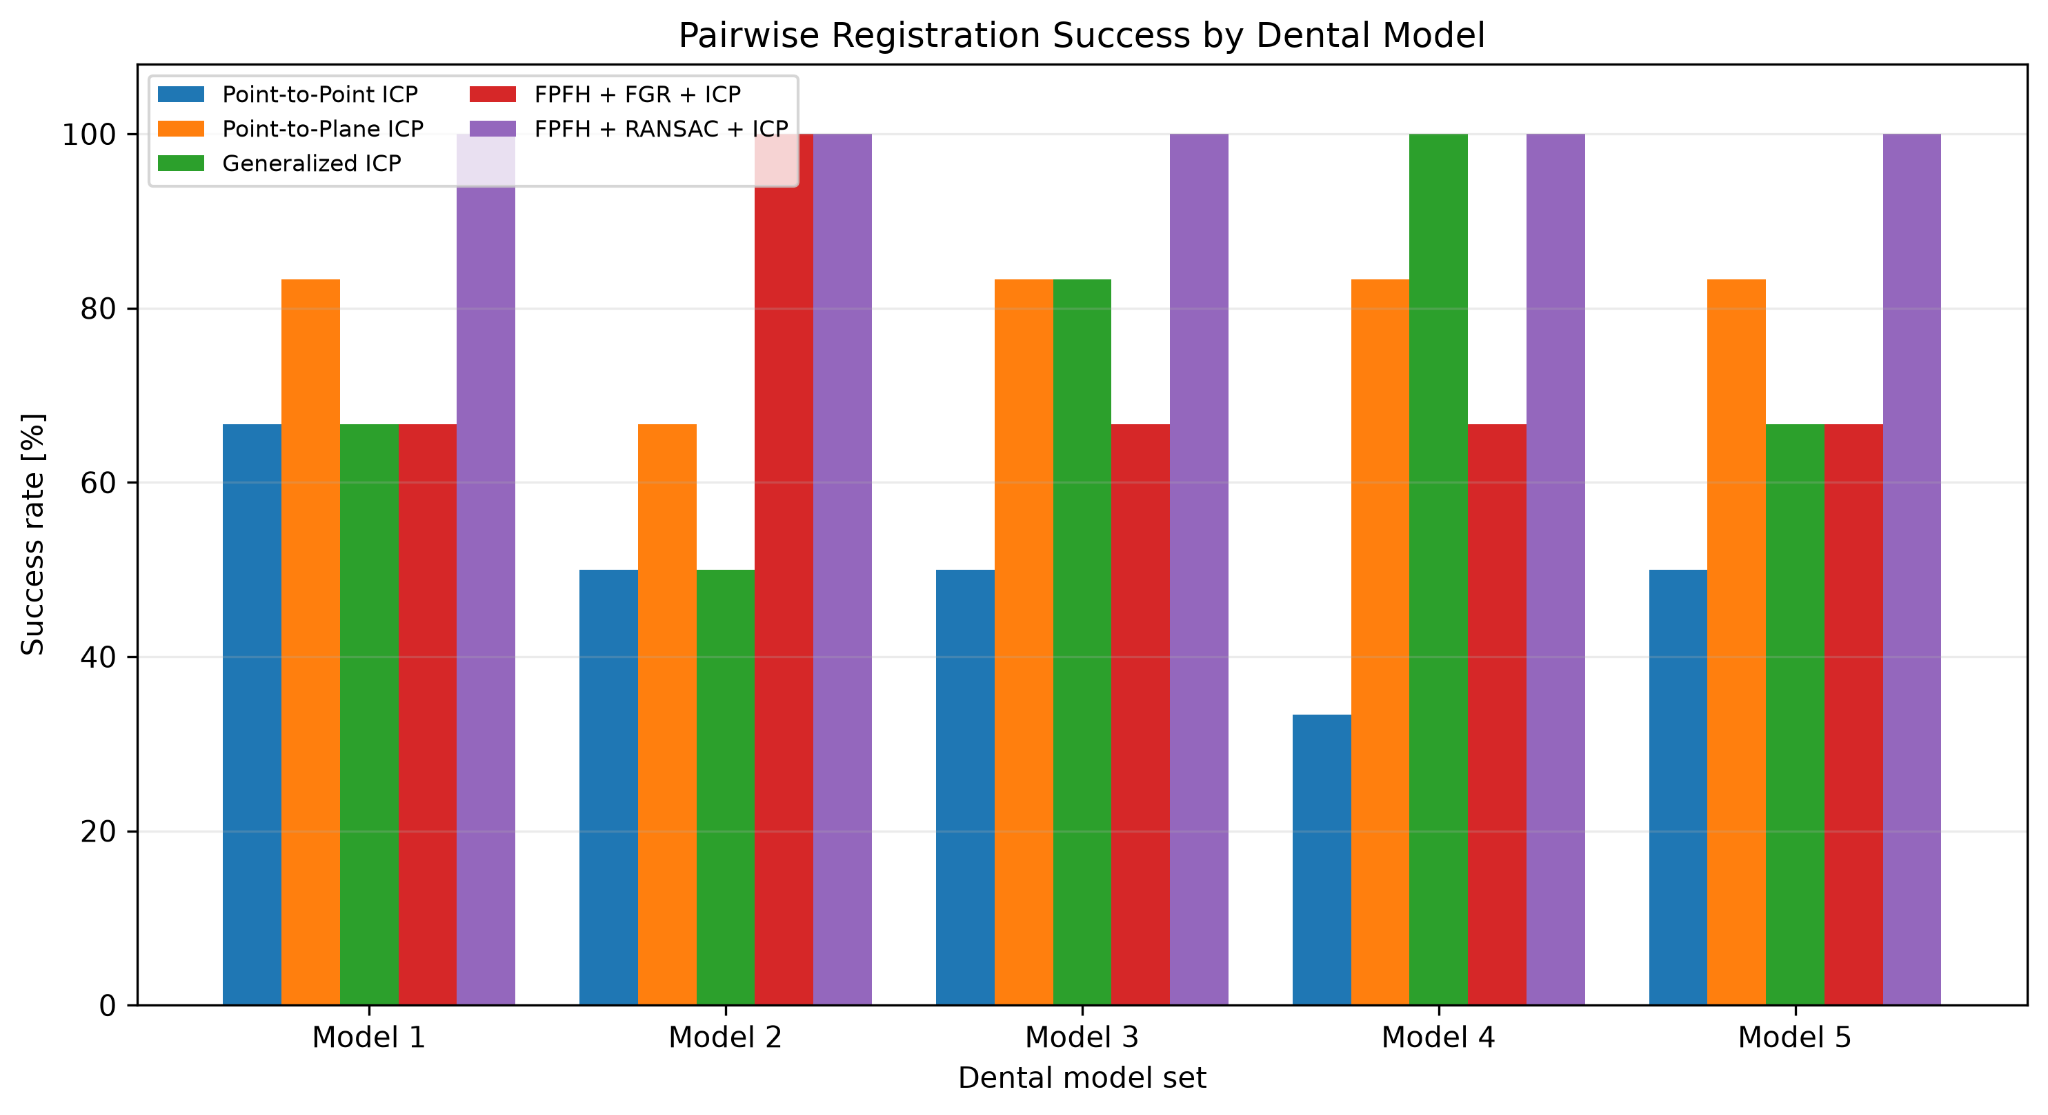
\includegraphics[width=\linewidth]{assets/marvin/model_suite/model_suite_pairwise_success_by_model.png}
    \caption{Success separated by model set.}
\end{subfigure}
\caption{Five-model zero-noise pairwise validation. RANSAC + ICP achieved 30/30 successful registrations and 100\% success in every individual model set.}
\label{fig:model-suite-pairwise}
\end{figure*}

The five-model experiment makes the distinction between precision and robustness particularly clear. FGR + ICP and GICP have very small median errors when they converge correctly, yet their much larger mean errors reveal severe outliers. RANSAC + ICP combines similarly low successful-case error with no failures in the 30 evaluated adjacent-fragment cases. The 100\% observed rate corresponds to 30/30 cases and is reported as a benchmark result rather than as evidence of universal reliability.


\begin{figure}[!t]
    \centering
    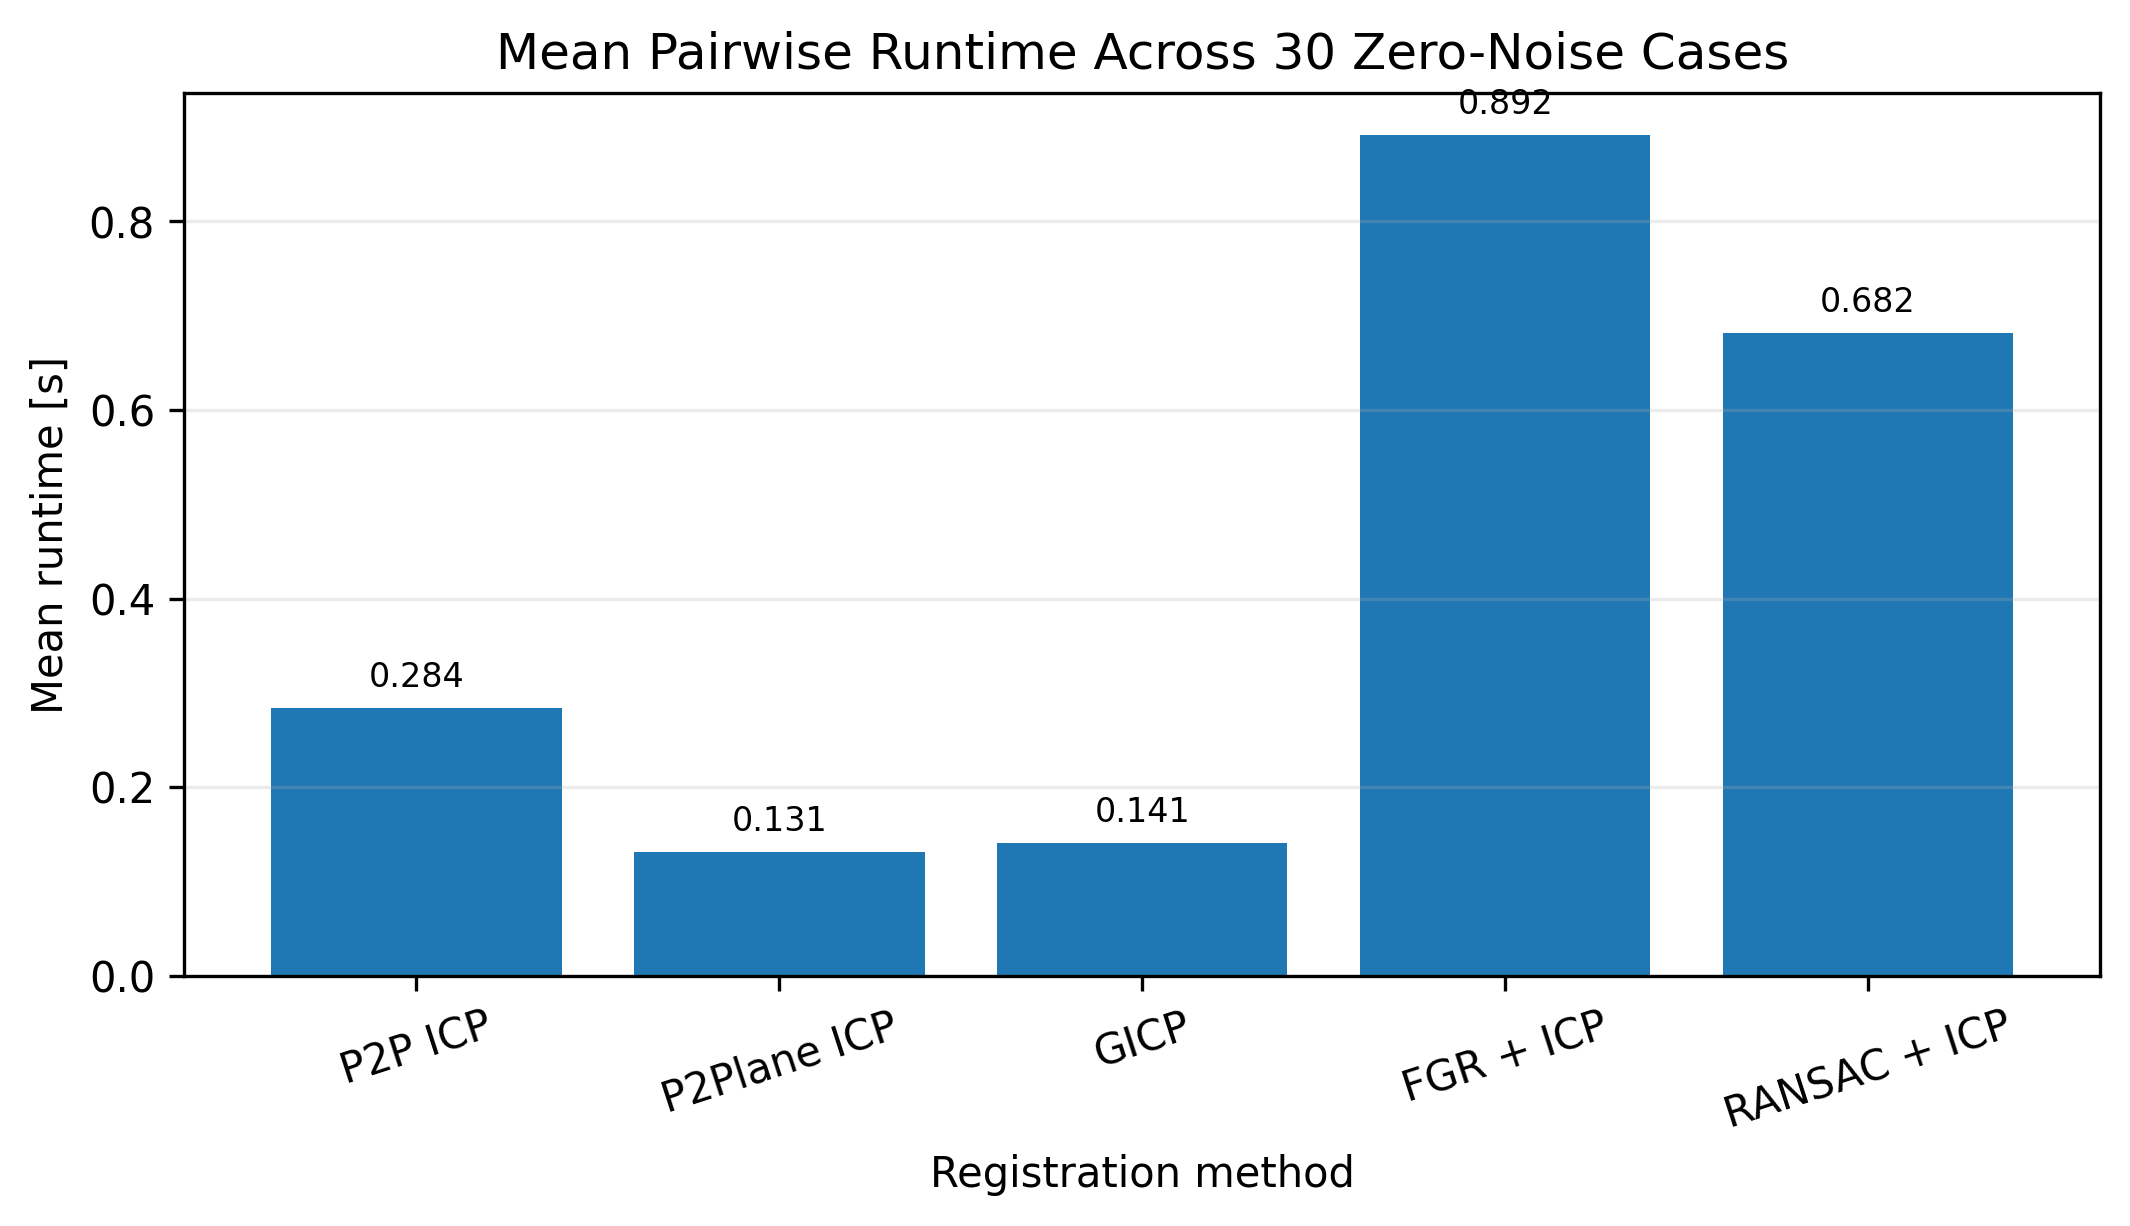
\includegraphics[width=\columnwidth]{assets/marvin/model_suite/model_suite_pairwise_runtime.png}
    \caption{Mean runtime per zero-noise adjacent-pair registration across the 30 realistic cases. The selected RANSAC pipeline is slower than the local ICP variants but remains below FGR in this benchmark while providing substantially higher robustness.}
    \label{fig:model-suite-runtime}
\end{figure}

Runtime therefore represents a real but acceptable trade-off rather than a hidden cost. Point-to-Plane ICP and GICP are fastest at approximately 0.13--0.14~s per evaluated pair, whereas RANSAC + ICP requires about 0.68~s and FGR + ICP about 0.89~s on the benchmark system. The selected RANSAC pipeline is roughly five times slower than the fastest local methods, but those local methods fail on 20--27\% of the zero-noise cases. Since a failed global alignment propagates directly into the subsequent multiway reconstruction, robustness was prioritized over sub-second differences in pairwise runtime.

\subsubsection{Noise Robustness Across Five Models}

Additive isotropic Gaussian positional noise was applied with standard deviations $0$, $0.01$, $0.025$, $0.05$, $0.10$, and $0.20$. At $\sigma=0$, each of the 30 distinct pairwise cases was evaluated once. At every nonzero level, three independent noise realizations were generated for each case, yielding 90 trials per algorithm and noise level. Within a given realization, all algorithms receive exactly the same noisy point clouds.

\begin{figure*}[!t]
    \centering
    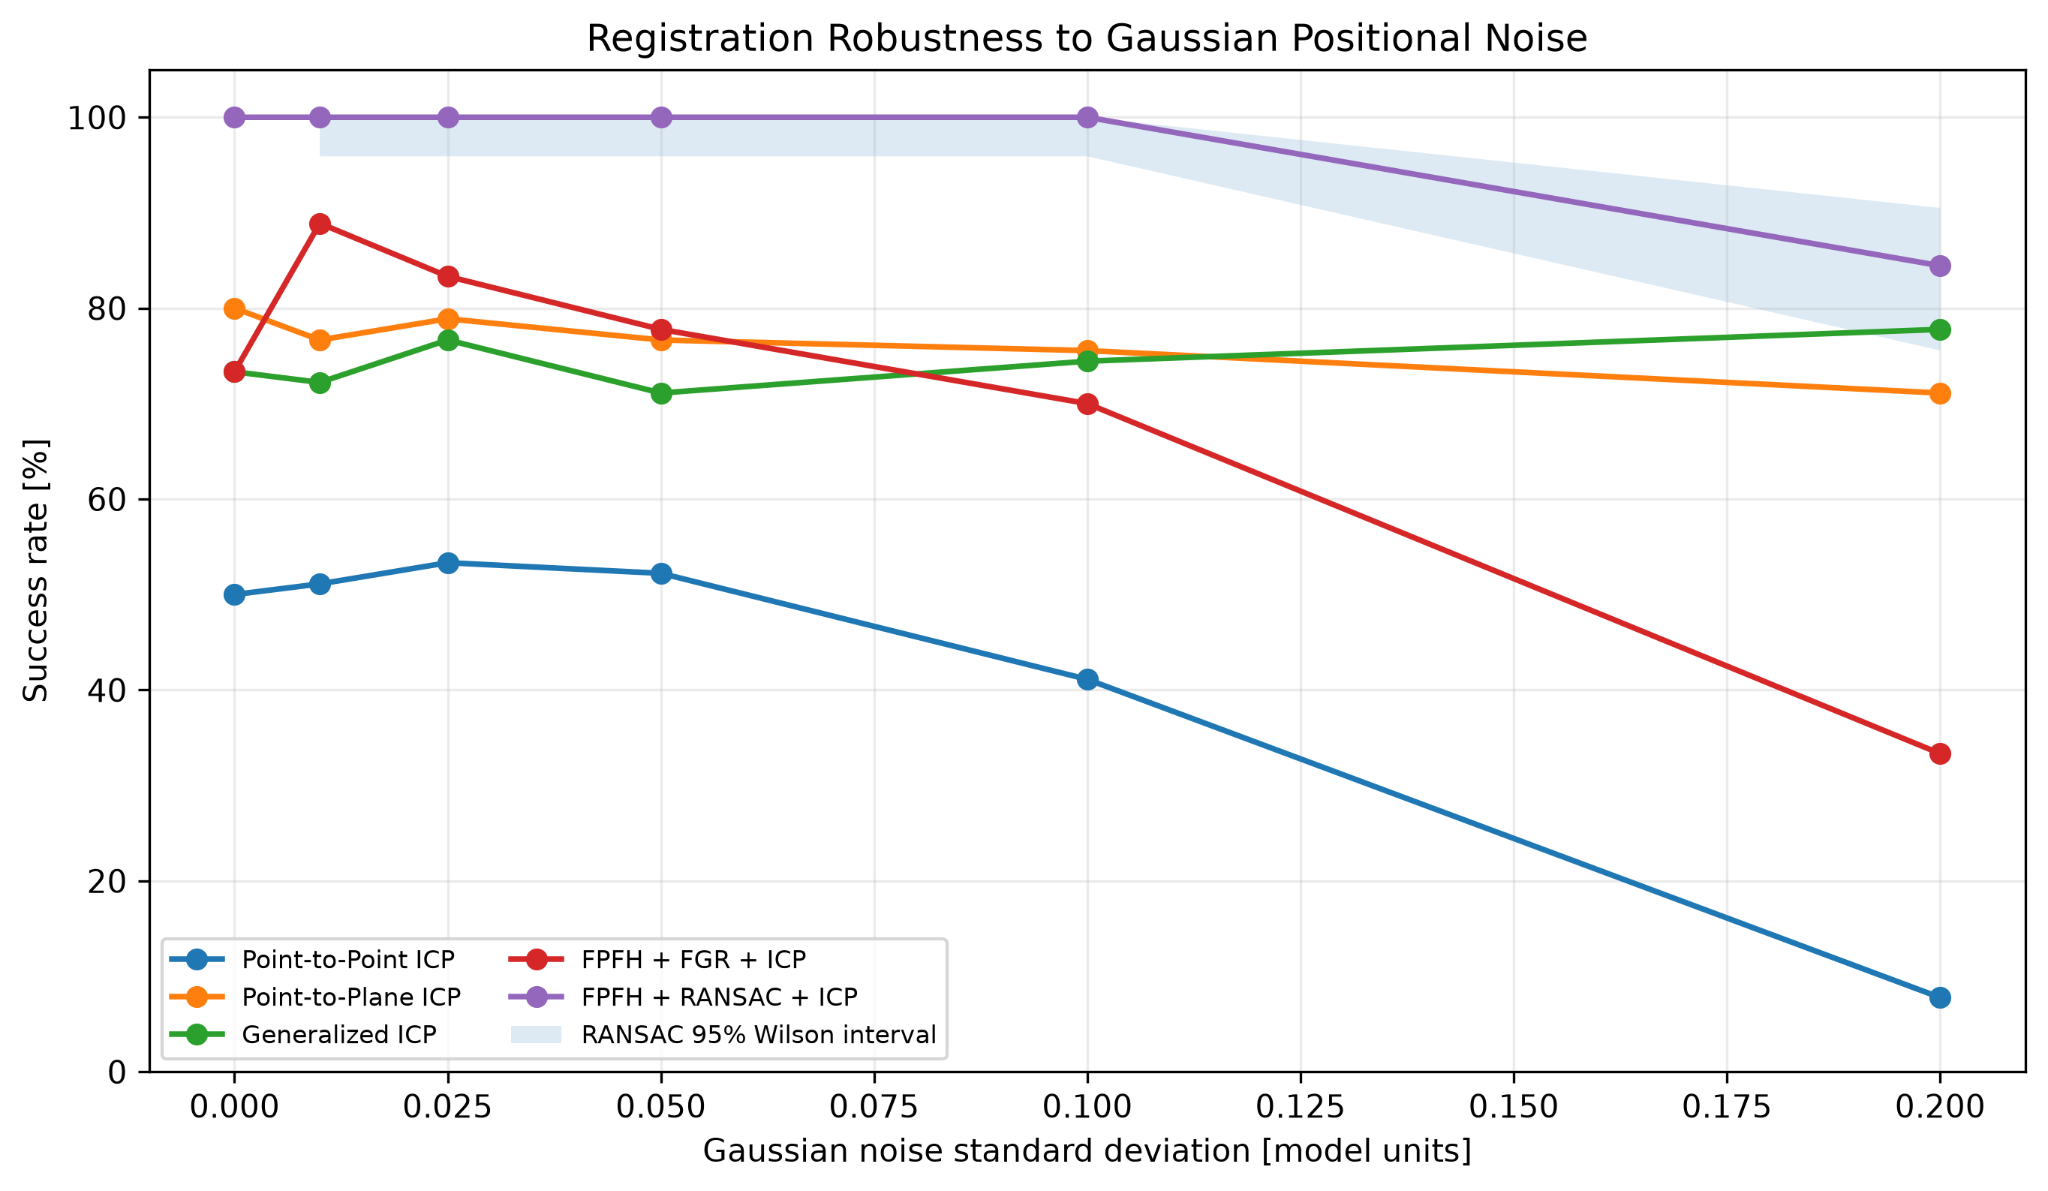
\includegraphics[width=0.82\textwidth]{assets/marvin/model_suite/model_suite_noise_success_rate.png}
    \caption{Success rate under additive Gaussian positional noise across five dental model sets. The shaded band shows the 95\% Wilson interval for RANSAC + ICP at nonzero noise levels. Because repeated noise realizations share the same 30 underlying fragment pairs, the intervals are used as descriptive finite-sample uncertainty indicators rather than formal population-level confidence statements.}
    \label{fig:model-suite-noise}
\end{figure*}

\begin{table}[H]
\centering
\footnotesize
\setlength{\tabcolsep}{3pt}
\begin{tabular}{rrrrrr}
\toprule
$\sigma$ & \textbf{P2P} & \textbf{P2Plane} & \textbf{GICP} & \textbf{FGR} & \textbf{RANSAC} \\
\midrule
0.000 & 50.0 & 80.0 & 73.3 & 73.3 & \textbf{100.0} \\
0.010 & 51.1 & 76.7 & 72.2 & 88.9 & \textbf{100.0} \\
0.025 & 53.3 & 78.9 & 76.7 & 83.3 & \textbf{100.0} \\
0.050 & 52.2 & 76.7 & 71.1 & 77.8 & \textbf{100.0} \\
0.100 & 41.1 & 75.6 & 74.4 & 70.0 & \textbf{100.0} \\
0.200 & 7.8 & 71.1 & 77.8 & 33.3 & \textbf{84.4} \\
\bottomrule
\end{tabular}
\caption{Success rate [\%] in the five-model noise study. The zero-noise row contains 30 unique cases; every nonzero row contains 90 noisy trials per algorithm.}
\label{tab:model-suite-noise}
\end{table}

RANSAC + ICP remained at 100\% observed success through $\sigma=0.10$. At $\sigma=0.20$, 76 of 90 trials succeeded, corresponding to 84.44\% and a Wilson interval of approximately 75.57--90.50\%. At the same level FGR dropped to 33.3\%, while GICP and Point-to-Plane ICP reached 77.8\% and 71.1\%, respectively. The RANSAC mean translation and rotation errors at $\sigma=0.10$ were only 0.02285 model units and $0.0898^\circ$. At $\sigma=0.20$, the mean errors rose to 0.4002 model units and $2.749^\circ$, whereas the corresponding medians remained much smaller at 0.1634 and $0.522^\circ$. This mean-to-median separation indicates that the strongest-noise condition is dominated by a subset of catastrophic failures rather than by a uniform loss of precision.


A second non-monotonic effect appears for FGR at very low noise: its observed success rate rises from 73.3\% at $\sigma=0$ to 88.9\% at $\sigma=0.01$ before decreasing again as the perturbation grows. This should not be interpreted as evidence that additive noise generally improves FGR. A plausible dataset-specific explanation is that small perturbations slightly change local neighborhoods and therefore FPFH descriptors, which can disrupt ambiguous feature correspondences produced by repetitive dental geometry and occasionally move the global optimization toward a more favorable hypothesis. At larger noise levels, descriptor degradation dominates and performance declines. Because the 90 nonzero-noise trials are repeated perturbations of the same 30 base pairs, this pattern is treated as a descriptive observation rather than as a statistically independent demonstration of a beneficial-noise effect.

\begin{samepage}
The expanded realistic validation therefore confirms the final pairwise choice:
\begin{center}
\textbf{FPFH $\rightarrow$ RANSAC $\rightarrow$ Point-to-Plane ICP.}
\end{center}
\end{samepage}

\subsection{Multiway Registration}
\label{sec:marvin-multiway}

The selected RANSAC + ICP pipeline was applied sequentially to the four fragments of every jaw. Pairwise transformations were chained into the reference coordinate system of fragment 0 without loop-closure correction, so the experiment directly measures accumulated odometry error. For pairwise transformation $T_{i\rightarrow i+1}$ and global pose $P_i$,
\begin{equation}
    P_{i+1} = P_i T_{i\rightarrow i+1}^{-1}.
\end{equation}
Because all acquisition transformations are known, each chained pose can be compared directly with ground truth.

\begin{figure*}[!t]
\centering
\begin{subfigure}[t]{0.48\textwidth}
    \centering
    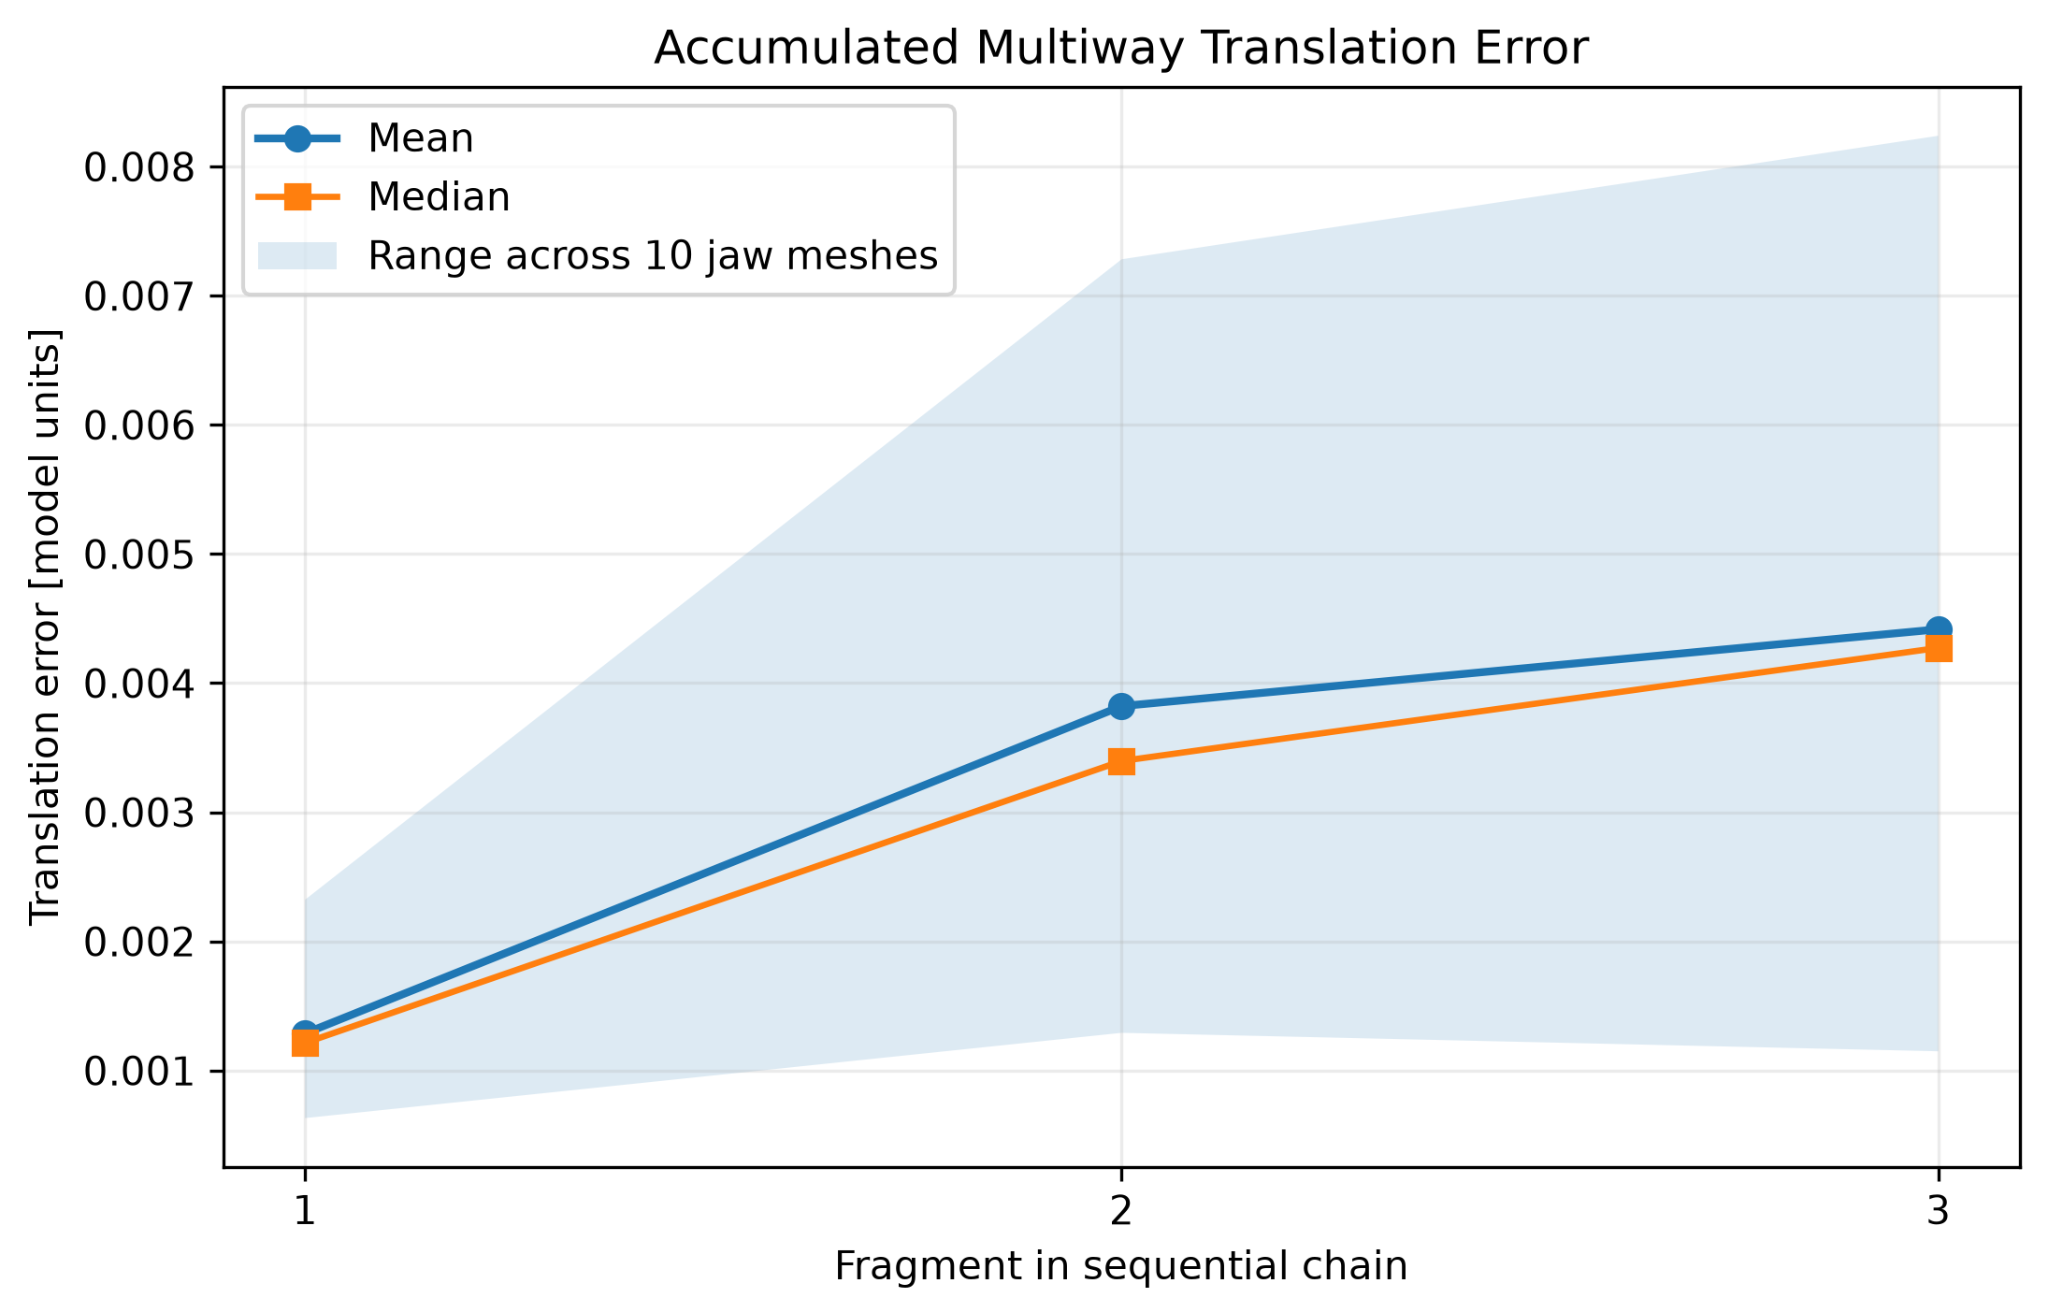
\includegraphics[width=\linewidth]{assets/marvin/model_suite/model_suite_multiway_translation_error.png}
    \caption{Accumulated translation error.}
\end{subfigure}\hfill
\begin{subfigure}[t]{0.48\textwidth}
    \centering
    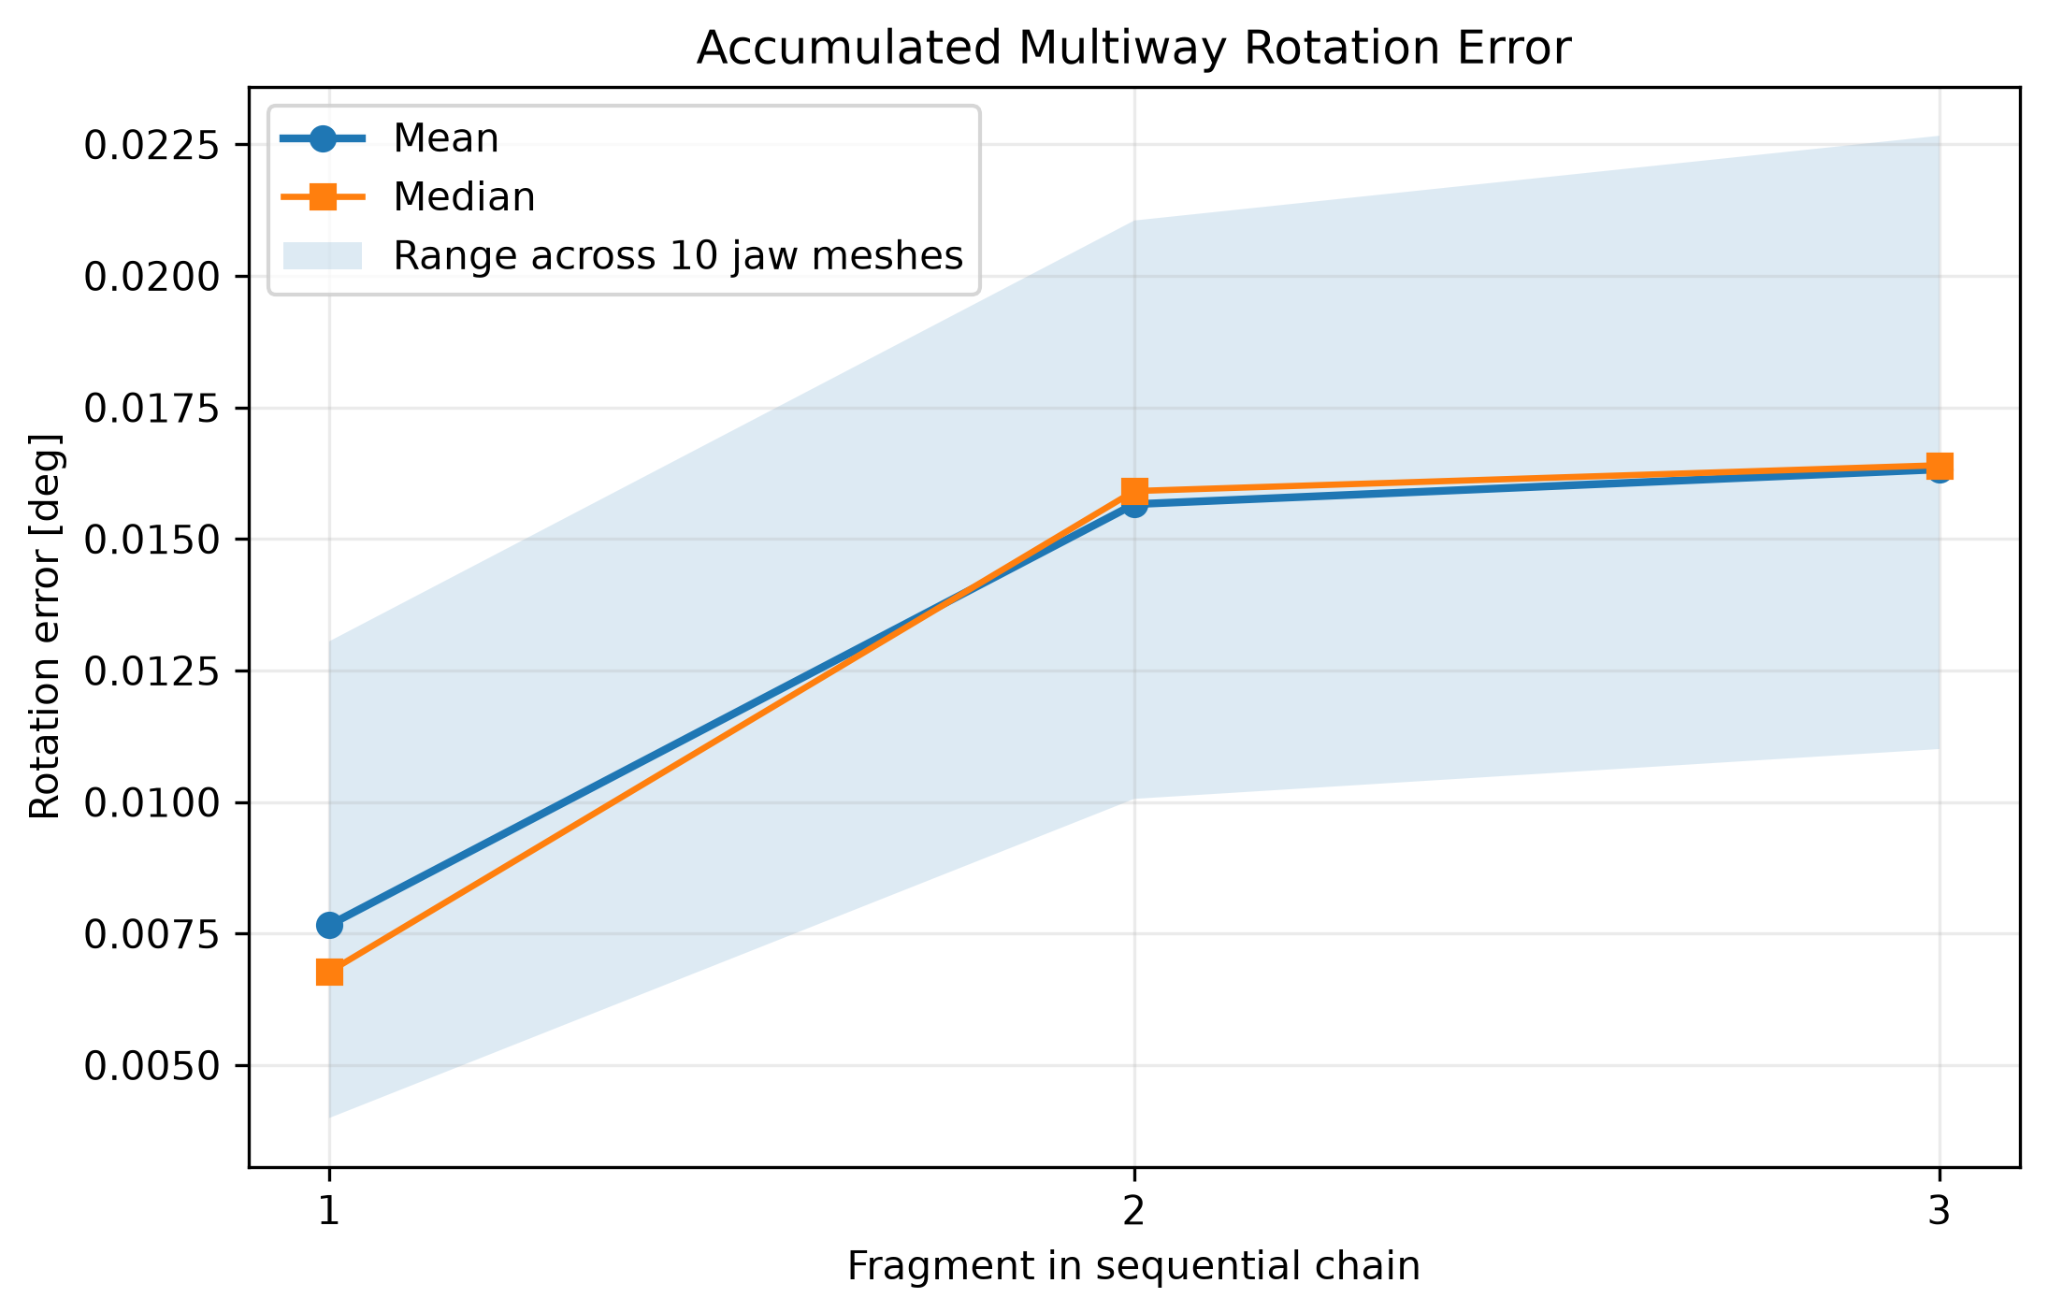
\includegraphics[width=\linewidth]{assets/marvin/model_suite/model_suite_multiway_rotation_error.png}
    \caption{Accumulated rotation error.}
\end{subfigure}
\caption{Sequential multiway error across all ten jaw meshes. Lines show mean and median; shaded regions show the full range across the ten jaws.}
\label{fig:model-suite-multiway-errors}
\end{figure*}

\begin{table}[H]
\centering
\footnotesize
\begin{tabularx}{\columnwidth}{@{}lYYY@{}}
\toprule
\textbf{Metric} & \textbf{Mean} & \textbf{Median} & \textbf{Maximum} \\
\midrule
Translation error [model units] & 0.003175 & 0.003059 & 0.008239 \\
Rotation error [$^\circ$] & 0.013212 & 0.013768 & 0.022660 \\
\bottomrule
\end{tabularx}
\caption{Global pose error over 30 non-reference poses from ten sequential four-fragment registrations.}
\label{tab:model-suite-multiway-overall}
\end{table}

The pairwise middle edge $1\rightarrow2$ remains the most difficult odometry step across the model suite: its mean pairwise rotation error is $0.01310^\circ$, compared with $0.00766^\circ$ for $0\rightarrow1$ and $0.00758^\circ$ for $2\rightarrow3$. Even after sequential accumulation, however, the worst observed global pose error remains only 0.008239 model units in translation and $0.02266^\circ$ in rotation. The ten merged point clouds form the inputs to the surface-reconstruction validation.

\subsection{Surface Reconstruction}
\label{sec:marvin-surface-reconstruction}

A point cloud contains discrete surface samples but no explicit connectivity \cite{kraus_huang2024}. The model-construction stage therefore estimates a triangular surface from the registered points. Two methods were compared: Poisson Surface Reconstruction \cite{kraus_kazhdan2006} and the Ball Pivoting Algorithm \cite{kraus_bernardini1999}.

Poisson reconstruction solves for an implicit surface and tends to produce smooth, globally connected geometry. This is advantageous for completeness, but missing measurements may be bridged by surfaces that are not actually supported by the input points. Ball Pivoting constructs triangles locally by rolling virtual balls with specified radii over the oriented point cloud. It is therefore more conservative but may leave open boundaries when the selected radii are too small.

Normals are estimated using a radius equal to three times the mean nearest-neighbor distance and at most 50 neighbors. Poisson is evaluated at depth 9 with the lowest 2\% density vertices removed. BPA uses multiple radii relative to the mean point spacing.

For mesh evaluation, 100,000 points are sampled uniformly from the reconstructed surface. Distances are measured in both directions: input/reference $\rightarrow$ reconstructed mesh and reconstructed mesh $\rightarrow$ input/reference. The second direction is important because it reveals unsupported surface patches. The symmetric RMSE combines both directions:
\begin{equation}
    \mathrm{RMSE}_{sym} =
    \sqrt{\frac{\mathrm{RMSE}_{A\rightarrow B}^{2}+
    \mathrm{RMSE}_{B\rightarrow A}^{2}}{2}}.
\end{equation}
This is a sampling-based surface approximation rather than an exact point-to-triangle Hausdorff distance.

\begin{figure*}[!t]
\centering
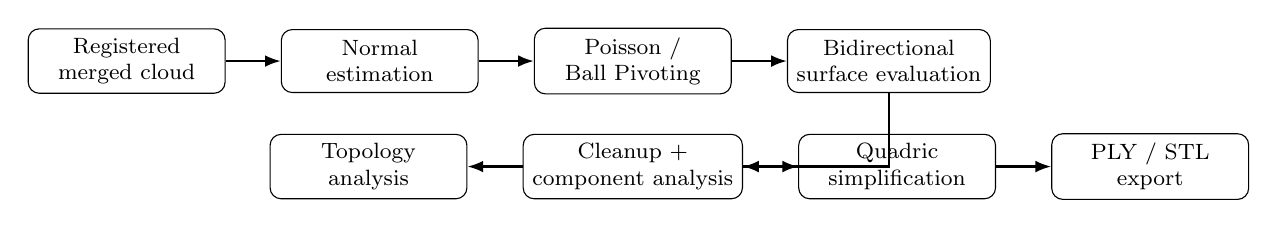
\begin{tikzpicture}[
    node distance=5mm and 7mm,
    box/.style={draw,rounded corners,align=center,minimum width=25mm,minimum height=8mm,font=\footnotesize},
    arr/.style={-{Latex[length=2mm]},thick}
]
\node[box] (cloud) {Registered\\merged cloud};
\node[box, right=of cloud] (norm) {Normal\\estimation};
\node[box, right=of norm] (methods) {Poisson /\\Ball Pivoting};
\node[box, right=of methods] (eval) {Bidirectional\\surface evaluation};
\node[box, below=of methods] (clean) {Cleanup +\\component analysis};
\node[box, left=of clean] (topo) {Topology\\analysis};
\node[box, right=of clean] (simp) {Quadric\\simplification};
\node[box, right=of simp] (export) {PLY / STL\\export};
\draw[arr] (cloud) -- (norm);
\draw[arr] (norm) -- (methods);
\draw[arr] (methods) -- (eval);
\draw[arr] (eval) |- (clean);
\draw[arr] (clean) -- (topo);
\draw[arr] (clean) -- (simp);
\draw[arr] (simp) -- (export);
\end{tikzpicture}
\caption{Surface-reconstruction and model-processing workflow. Algorithm selection is based on geometry and topology rather than visual smoothness alone.}
\label{fig:surface-reconstruction-workflow}
\end{figure*}

\subsection{Synthetic Mesh Evaluation}
\label{sec:marvin-synthetic-mesh}

\subsubsection{Poisson versus Ball Pivoting}

On the synthetic merged cloud containing 22,022 points, Poisson produced a dense surface but also a very large mesh-to-cloud error and self-intersections. The cleaned BPA reconstruction was much closer to the observed geometry.

\begin{table}[!t]
\centering
\footnotesize
\setlength{\tabcolsep}{3pt}
\begin{tabularx}{\columnwidth}{@{}lYY@{}}
\toprule
\textbf{Metric} & \textbf{Poisson} & \textbf{BPA} \\
\midrule
Triangles & 151,430 & 40,020 \\
Connected components & 17 & 1 \\
Self-intersections & Yes & No \\
Cloud $\rightarrow$ mesh RMSE & 0.122208 & 0.076404 \\
Mesh $\rightarrow$ cloud RMSE & 2.741374 & 0.115709 \\
Symmetric RMSE & 1.940369 & 0.098046 \\
\bottomrule
\end{tabularx}
\caption{Synthetic surface-reconstruction comparison after BPA cleanup.}
\label{tab:synthetic-mesh-comparison}
\end{table}

\begin{figure}[!t]
    \centering
    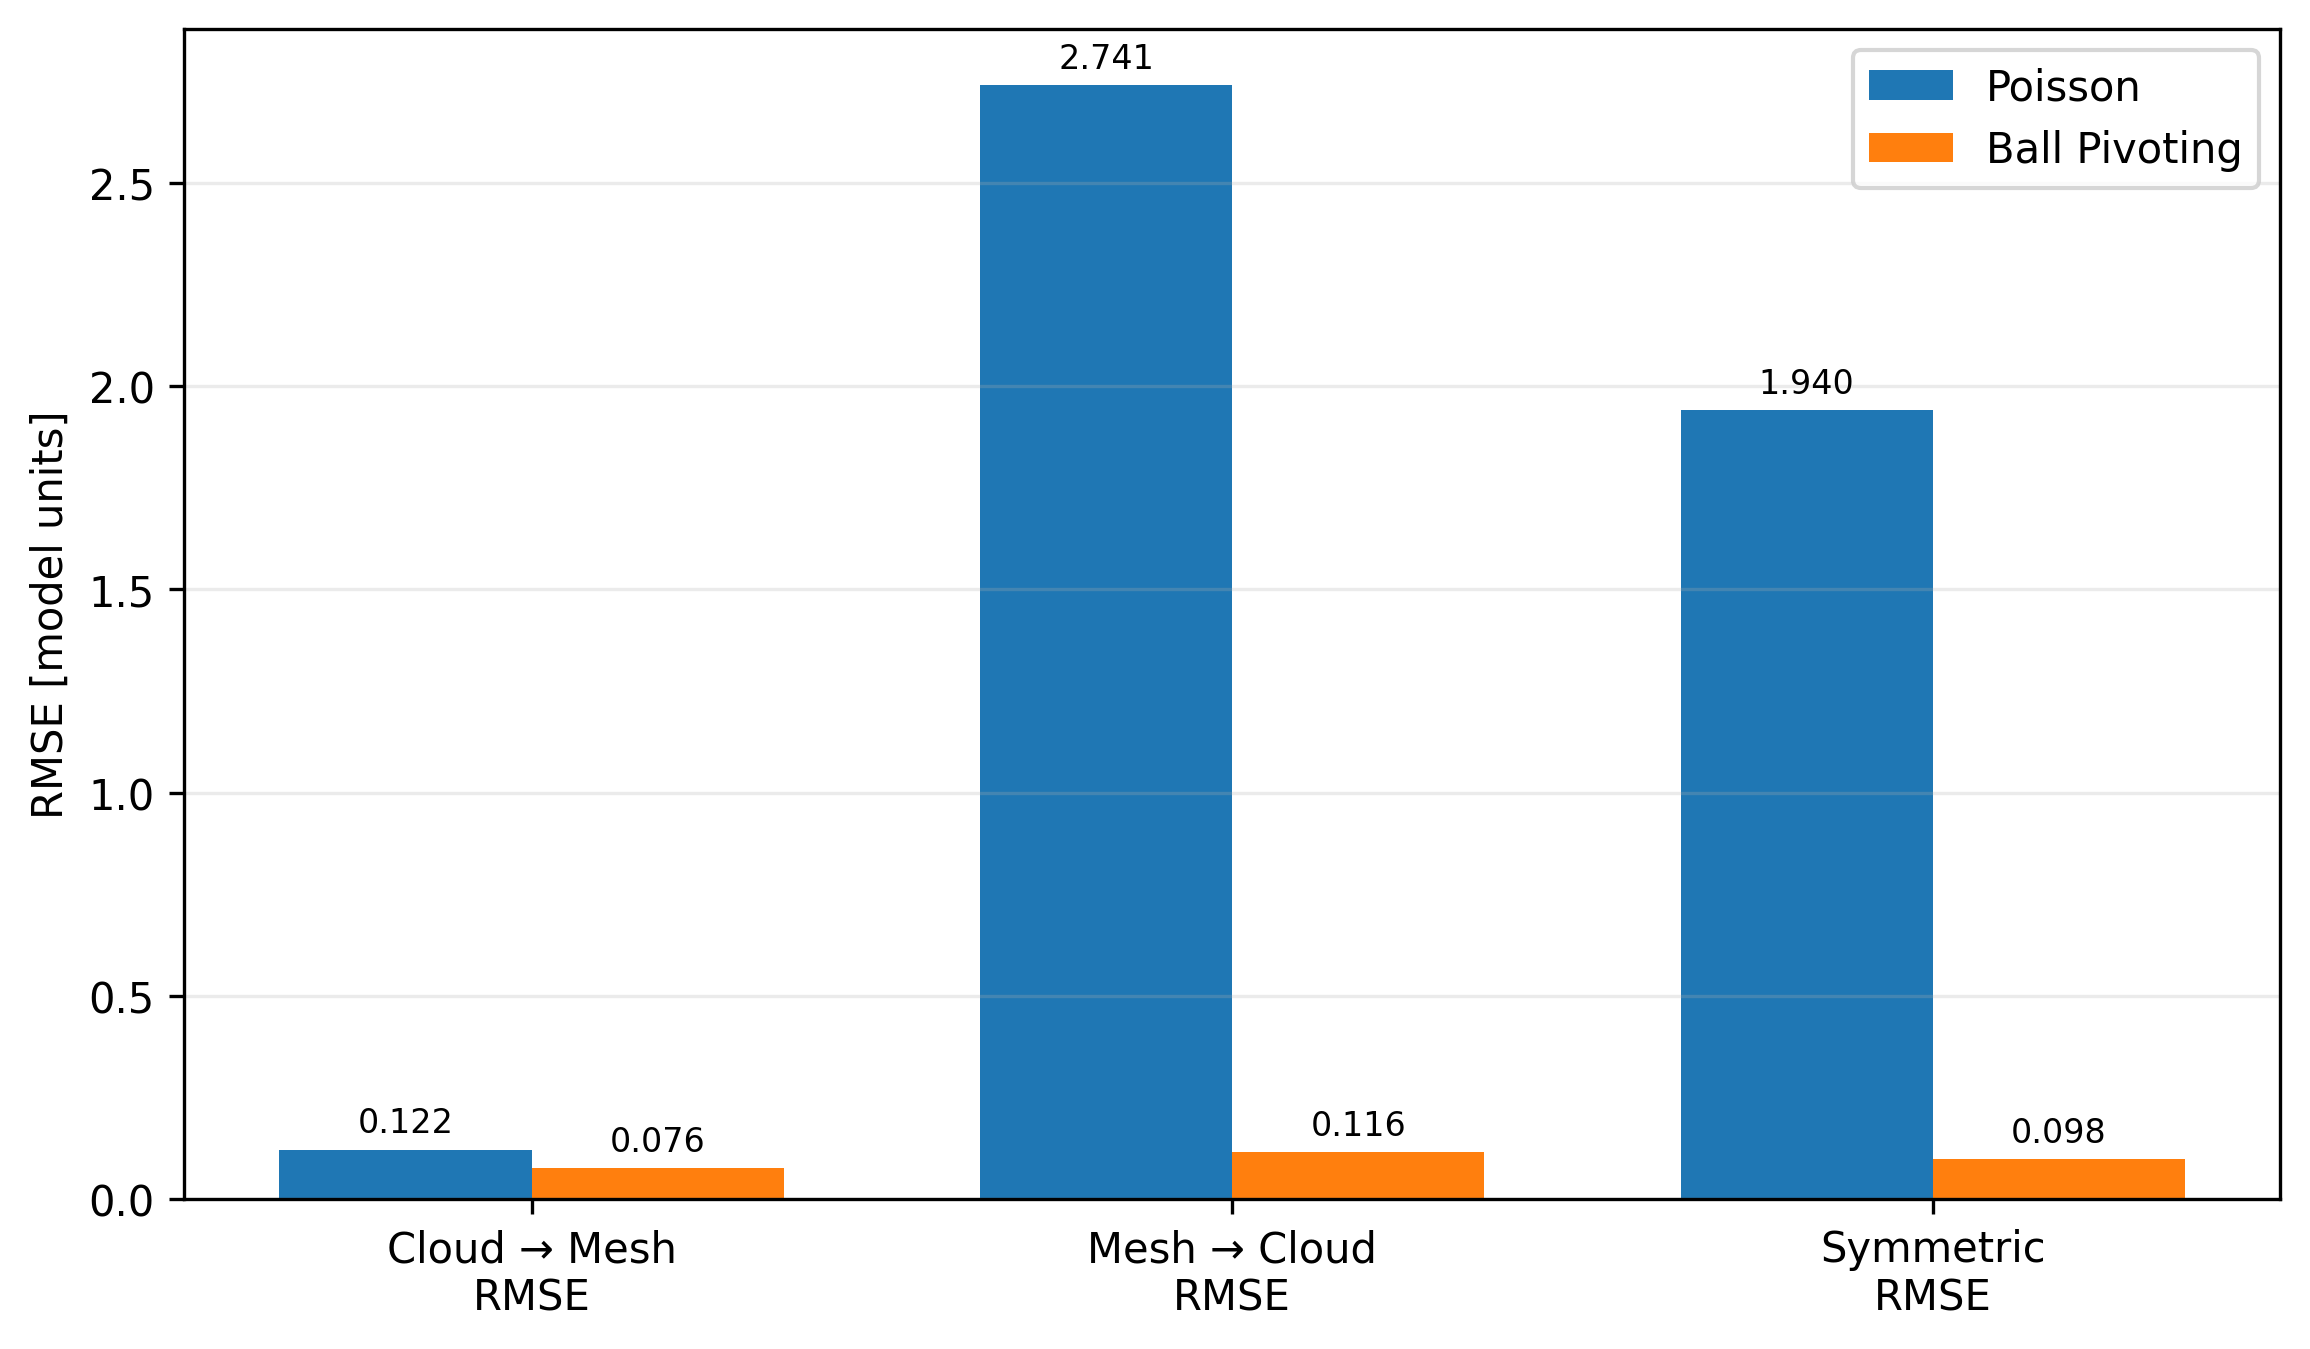
\includegraphics[width=0.92\linewidth]{assets/marvin/poisson_vs_ball_pivoting_rmse.png}
    \caption{Synthetic geometric error comparison between Poisson and Ball Pivoting.}
    \label{fig:synthetic-poisson-bpa}
\end{figure}

\subsubsection{BPA Parameter Study and Cleanup}

Four BPA radius-factor sets were compared. The smallest set $(1.0,1.5,2.0)$ achieved the lowest symmetric RMSE on the synthetic geometry. Although it initially produced 82 connected components, 99.04\% of all triangles belonged to one dominant component; the remaining components were tiny satellites. Removing components below 250 triangles yielded one connected component with 40,020 triangles.

\begin{figure}[!t]
    \centering
    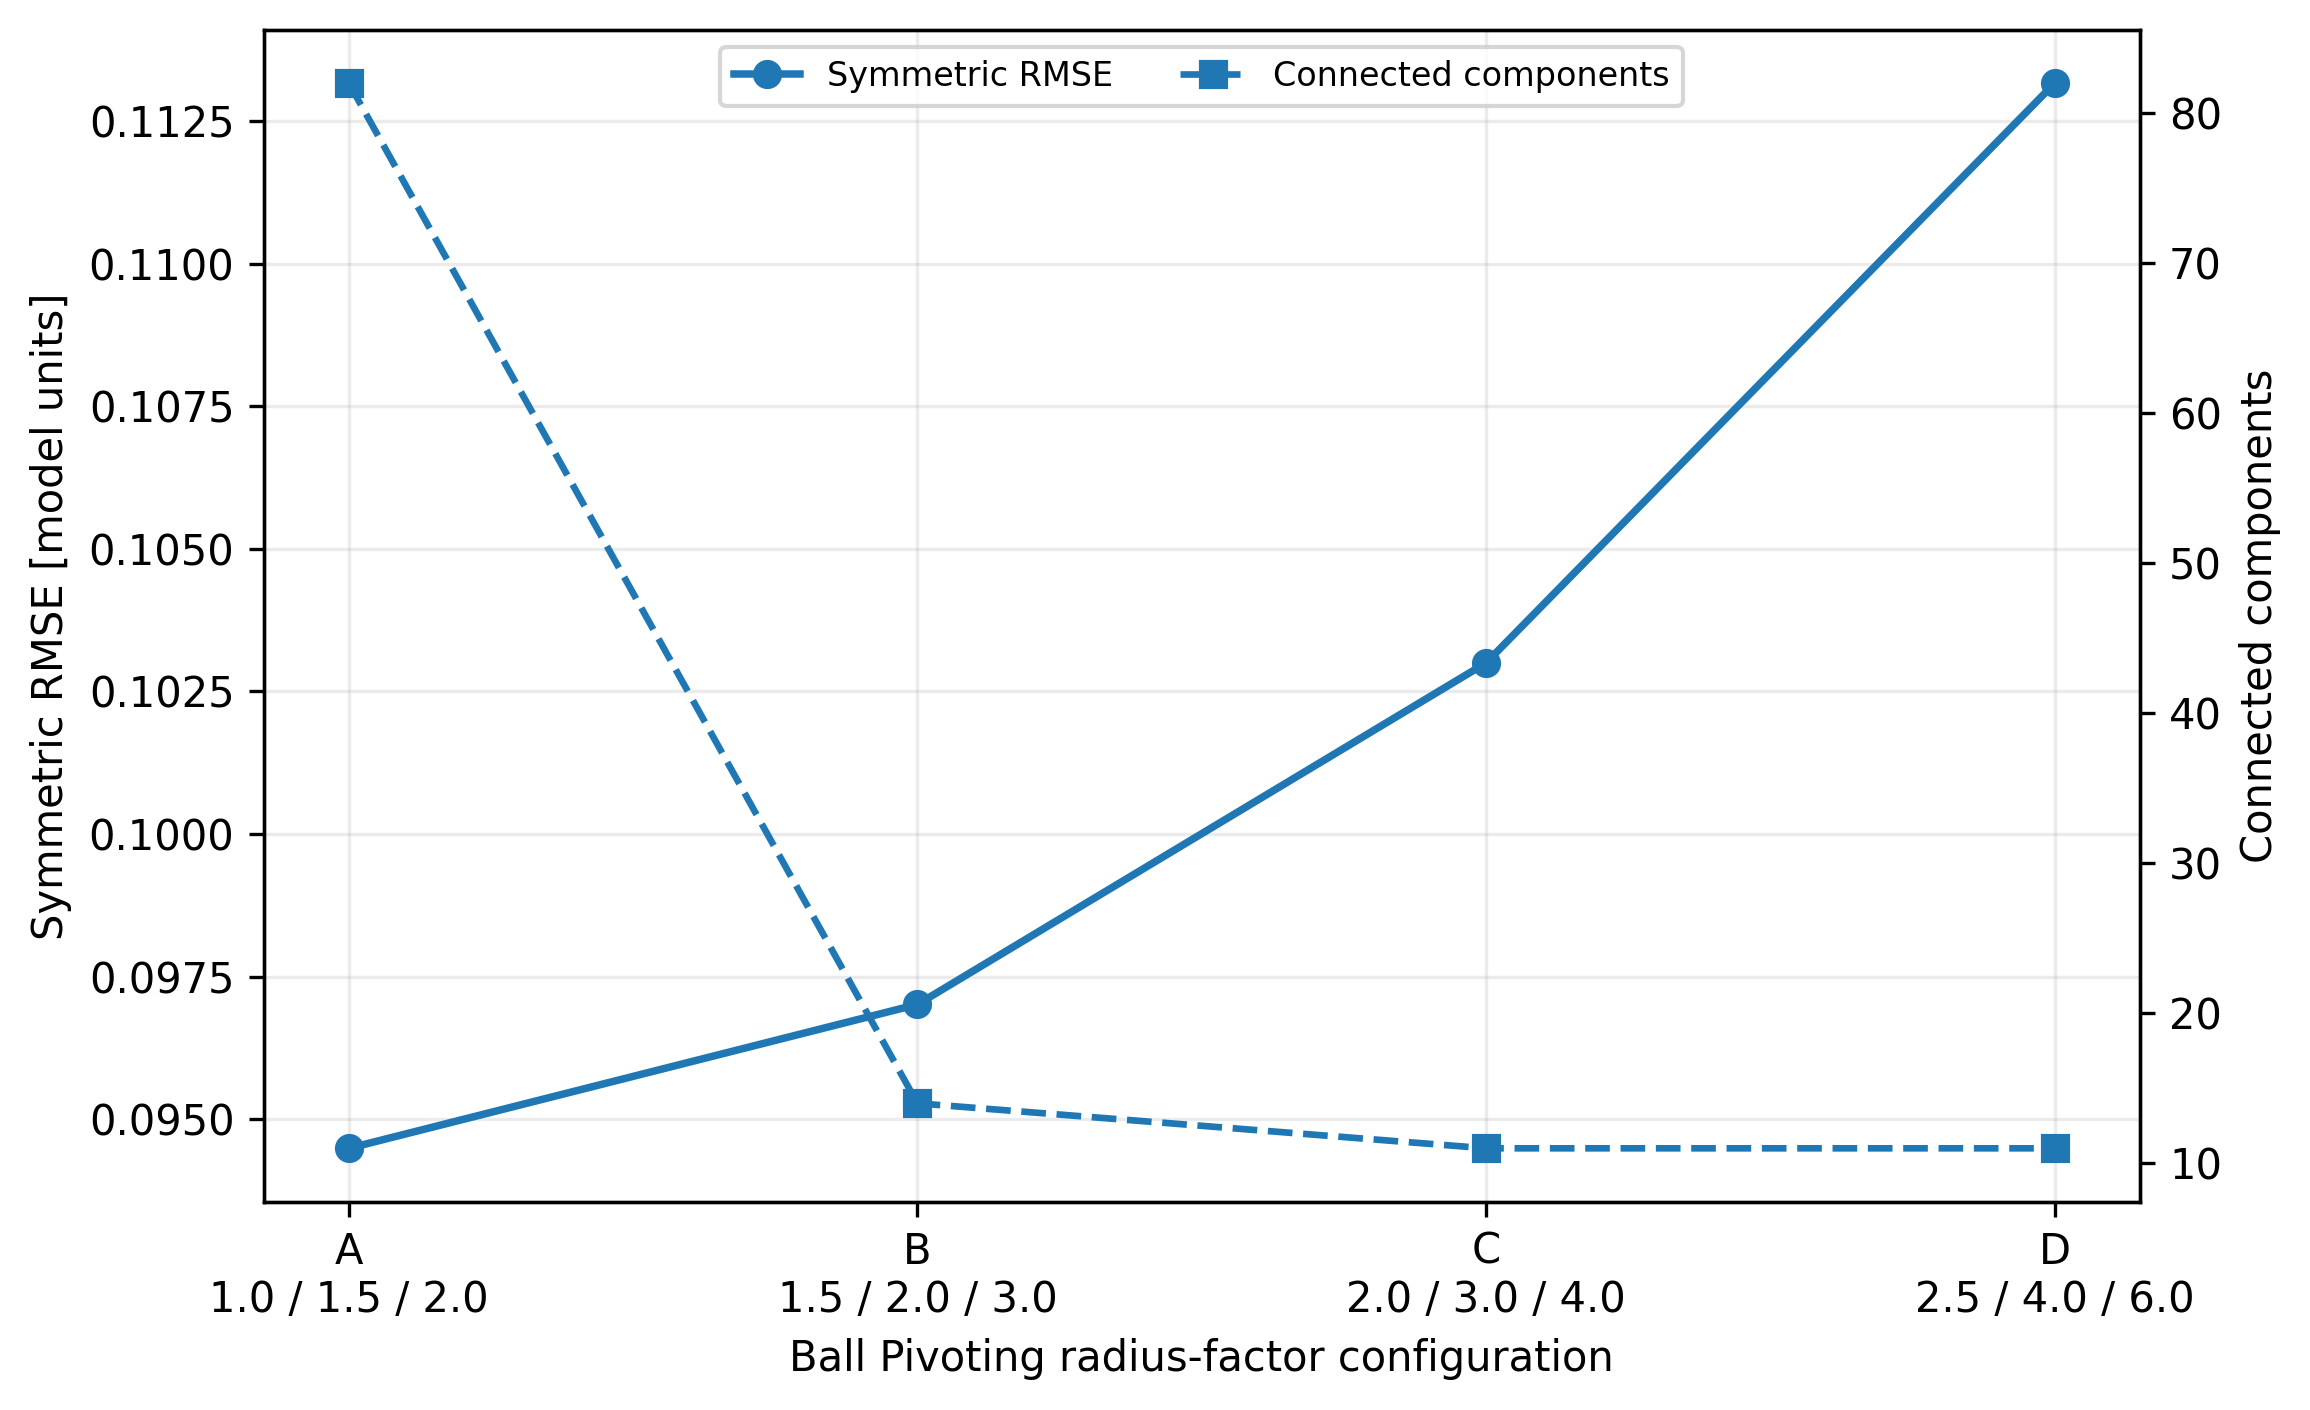
\includegraphics[width=0.92\linewidth]{assets/marvin/bpa_parameter_study.png}
    \caption{Synthetic BPA radius-factor study.}
    \label{fig:synthetic-bpa-study}
\end{figure}

A topology inspection identified no genuine non-manifold edges and no self-intersections, but the surface remained non-watertight, non-vertex-manifold, and globally non-orientable. An attempted vertex-splitting repair removed the non-manifold-vertex condition but introduced self-intersections. The repair was therefore rejected instead of forcing a topologically cleaner but geometrically worse result.

\begin{table}[!t]
\centering
\footnotesize
\begin{tabularx}{\columnwidth}{@{}lY@{}}
\toprule
\textbf{Topology property} & \textbf{Full-resolution BPA candidate} \\
\midrule
Vertices / triangles & 21,689 / 40,020 \\
Boundary edges & 7,982 \\
Non-manifold edges & 0 \\
Non-manifold vertices & 1,204 (5.55\%) \\
Self-intersections & 0 \\
Vertex manifold & No \\
Watertight & No \\
Orientable & No \\
Orientation-conflict edges & 420 \\
Affected triangles & 784 (1.96\%) \\
\bottomrule
\end{tabularx}
\caption{Detailed topology diagnosis of the cleaned synthetic BPA candidate.}
\label{tab:synthetic-topology}
\end{table}

\begin{table}[!t]
\centering
\footnotesize
\begin{tabularx}{\columnwidth}{@{}lYY@{}}
\toprule
\textbf{Property} & \textbf{Original} & \textbf{After vertex splitting} \\
\midrule
Vertices & 21,689 & 22,961 \\
Triangles & 40,020 & 40,020 \\
Non-manifold vertices & 1,204 & 0 \\
Vertex manifold & No & Yes \\
Self-intersections & No & \textbf{Yes} \\
Orientable & No & No \\
Symmetric RMSE & 0.098070 & 0.098070 \\
\bottomrule
\end{tabularx}
\caption{Rejected topology-repair attempt. Removing the non-manifold-vertex condition introduced self-intersections and was therefore not accepted.}
\label{tab:rejected-topology-repair}
\end{table}

\subsubsection{Mesh Simplification}

Quadric decimation \cite{kraus_garland1997} was tested at target sizes of 30,000, 20,000, 10,000, and 5,000 triangles. The 30k variant provided the best compromise: it reduced the triangle count by approximately 25\% while increasing the symmetric RMSE by only 0.171\%.

\begin{figure}[!t]
    \centering
    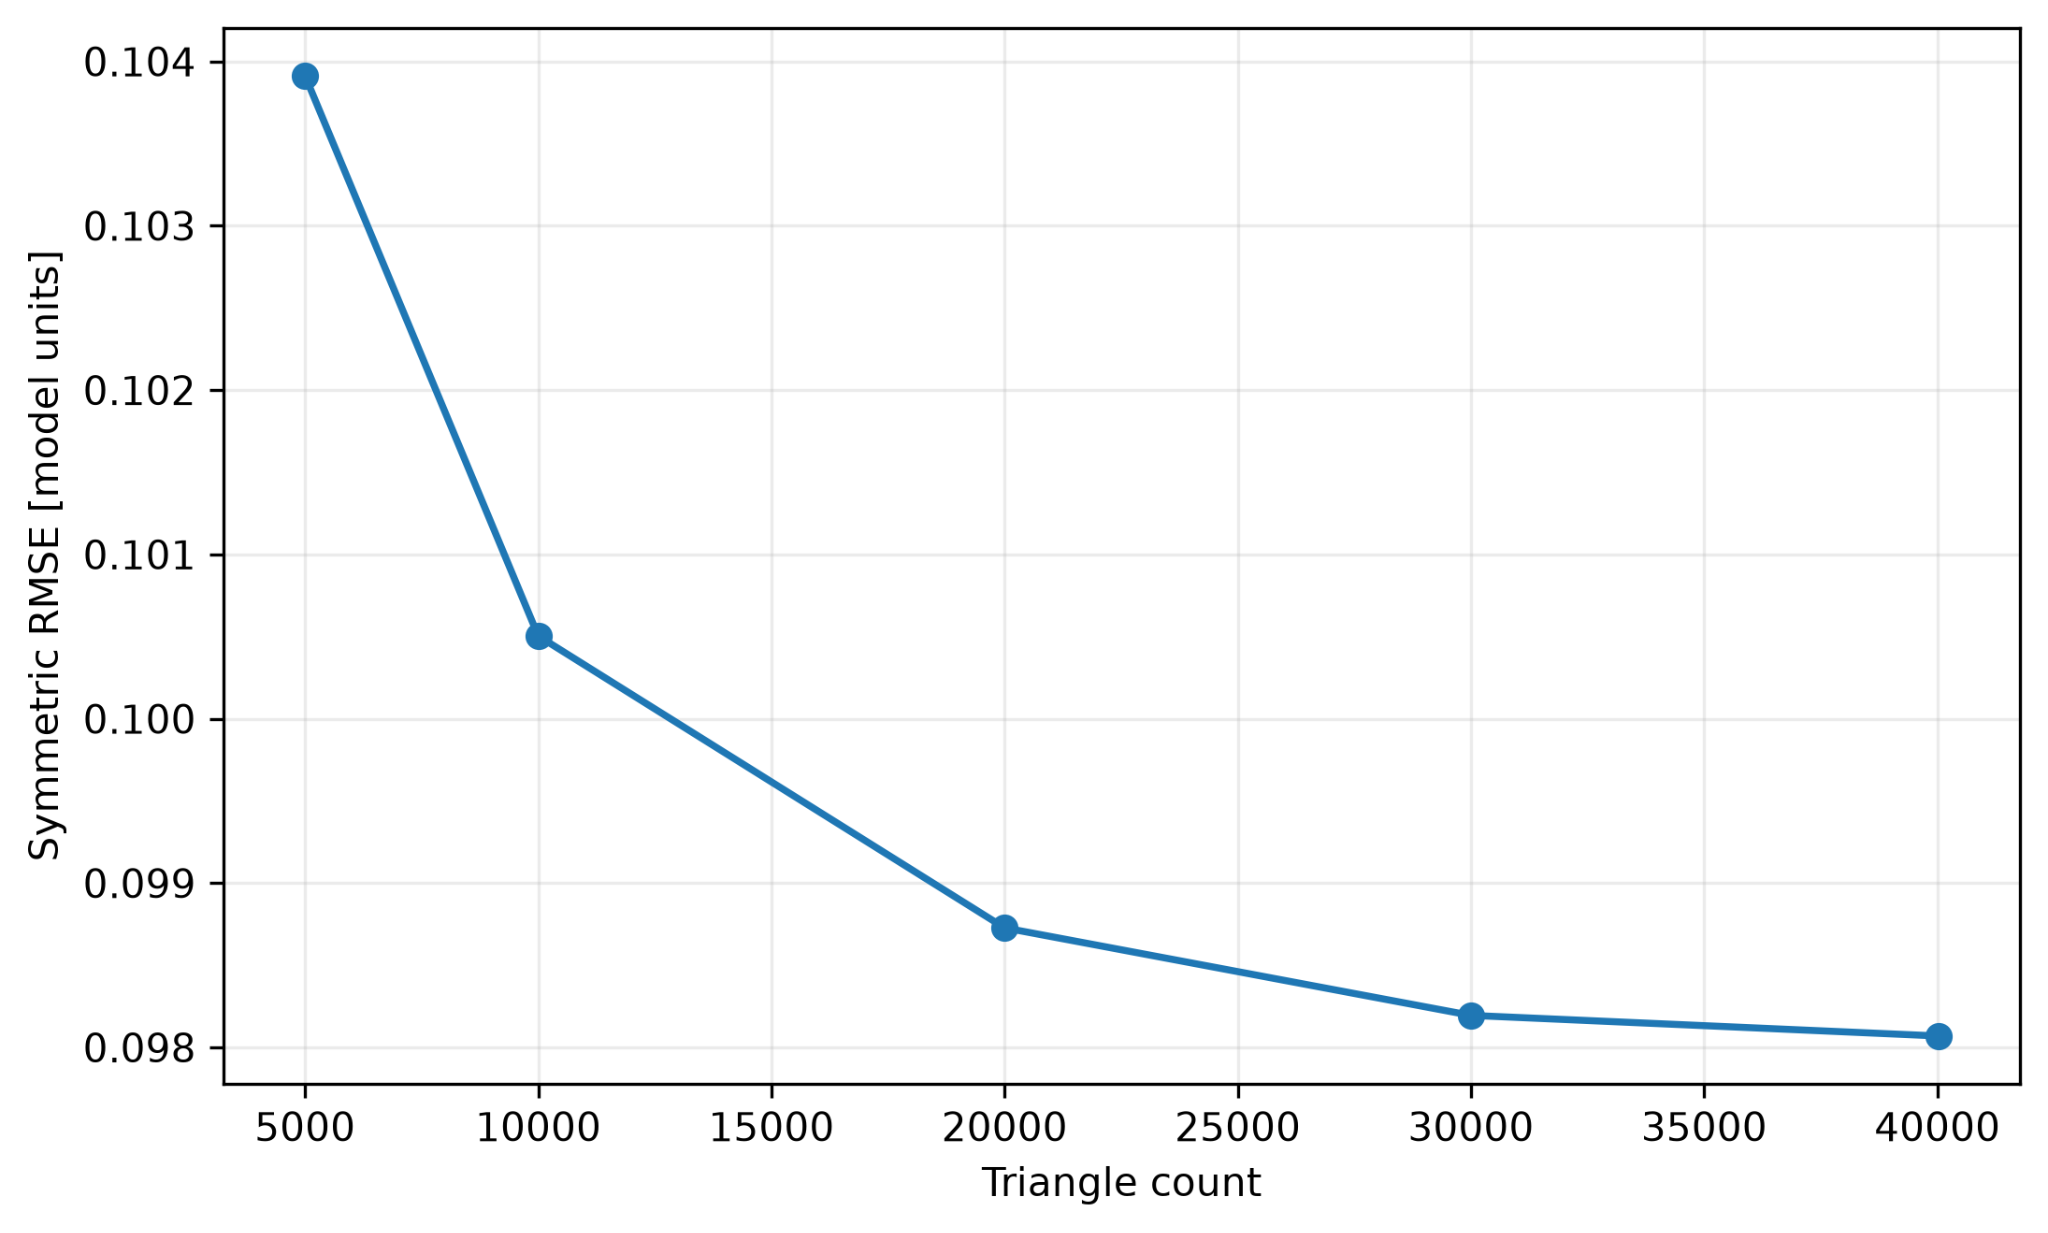
\includegraphics[width=0.92\linewidth]{assets/marvin/mesh_simplification_study.png}
    \caption{Synthetic mesh simplification study.}
    \label{fig:synthetic-simplification}
\end{figure}

\begin{table}[!t]
\centering
\footnotesize
\setlength{\tabcolsep}{3pt}
\begin{tabular}{lrrrr}
\toprule
\textbf{Variant} & \textbf{Triangles} & \textbf{Reduction} & \textbf{Components} & \textbf{Sym. RMSE} \\
\midrule
Original & 40,020 & 0.0\% & 1 & 0.098070 \\
30k & 29,999 & 25.0\% & 2 & 0.098195 \\
20k & 20,000 & 50.0\% & 19 & 0.098727 \\
10k & 10,000 & 75.0\% & 78 & 0.100504 \\
5k & 4,999 & 87.5\% & 46 & 0.103913 \\
\bottomrule
\end{tabular}
\caption{Synthetic simplification study. The 30k variant preserves geometry while stronger simplification rapidly increases fragmentation.}
\label{tab:synthetic-simplification}
\end{table}

After removing one isolated triangle, the final synthetic export contained 16,649 vertices and 29,998 triangles. The symmetric RMSE changed from 0.098070 for the full-resolution cleaned BPA mesh to 0.098237 after simplification and final cleanup, an increase of only 0.171\%. Both PLY and STL exports could be reloaded successfully. PLY reloaded with 16,649 indexed vertices and 29,998 triangles; STL retained the same triangle count but reported more vertices because STL repeats triangle vertices instead of storing the shared indexed connectivity used by PLY. This synthetic export pipeline demonstrates cleanup, simplification, serialization, and integrity checking independently of the later realistic-geometry validation.

\begin{table*}[!t]
\centering
\footnotesize
\begin{tabular}{lrrrrrrr}
\toprule
\textbf{Mesh} & \textbf{Vertices} & \textbf{Triangles} & \textbf{Components} & \textbf{Vertex manifold} & \textbf{Self-int.} & \textbf{Watertight} & \textbf{Sym. RMSE} \\
\midrule
Cleaned full-resolution BPA & 21,689 & 40,020 & 1 & No & No & No & 0.098070 \\
Final 30k export & 16,649 & 29,998 & 1 & No & No & No & 0.098237 \\
\bottomrule
\end{tabular}
\caption{Final synthetic mesh integrity check. Simplification reduces complexity substantially without creating self-intersections or materially changing geometric error.}
\label{tab:final-synthetic-quality}
\end{table*}

The remaining topological limitations are reported rather than hidden by aggressive repair. For visualization and geometric comparison the open BPA surface is acceptable, but applications requiring a closed volume would need a specialized downstream repair stage. This distinction is important for DentaVision: the current contribution targets faithful surface reconstruction, not guaranteed watertight solid modeling.

\subsection{Validation of Surface Reconstruction on Five Dental Models}
\label{sec:marvin-realistic-mesh}

\subsubsection{BPA Radius Re-Optimization Across Ten Jaws}

The realistic BPA parameter study was repeated on all ten registered jaw clouds. Four radius-factor configurations were evaluated against the original STL surfaces using symmetric RMSE, boundary-edge count, component structure, reconstructed-to-reference area ratio, and self-intersections.

\begin{figure*}[!t]
    \centering
    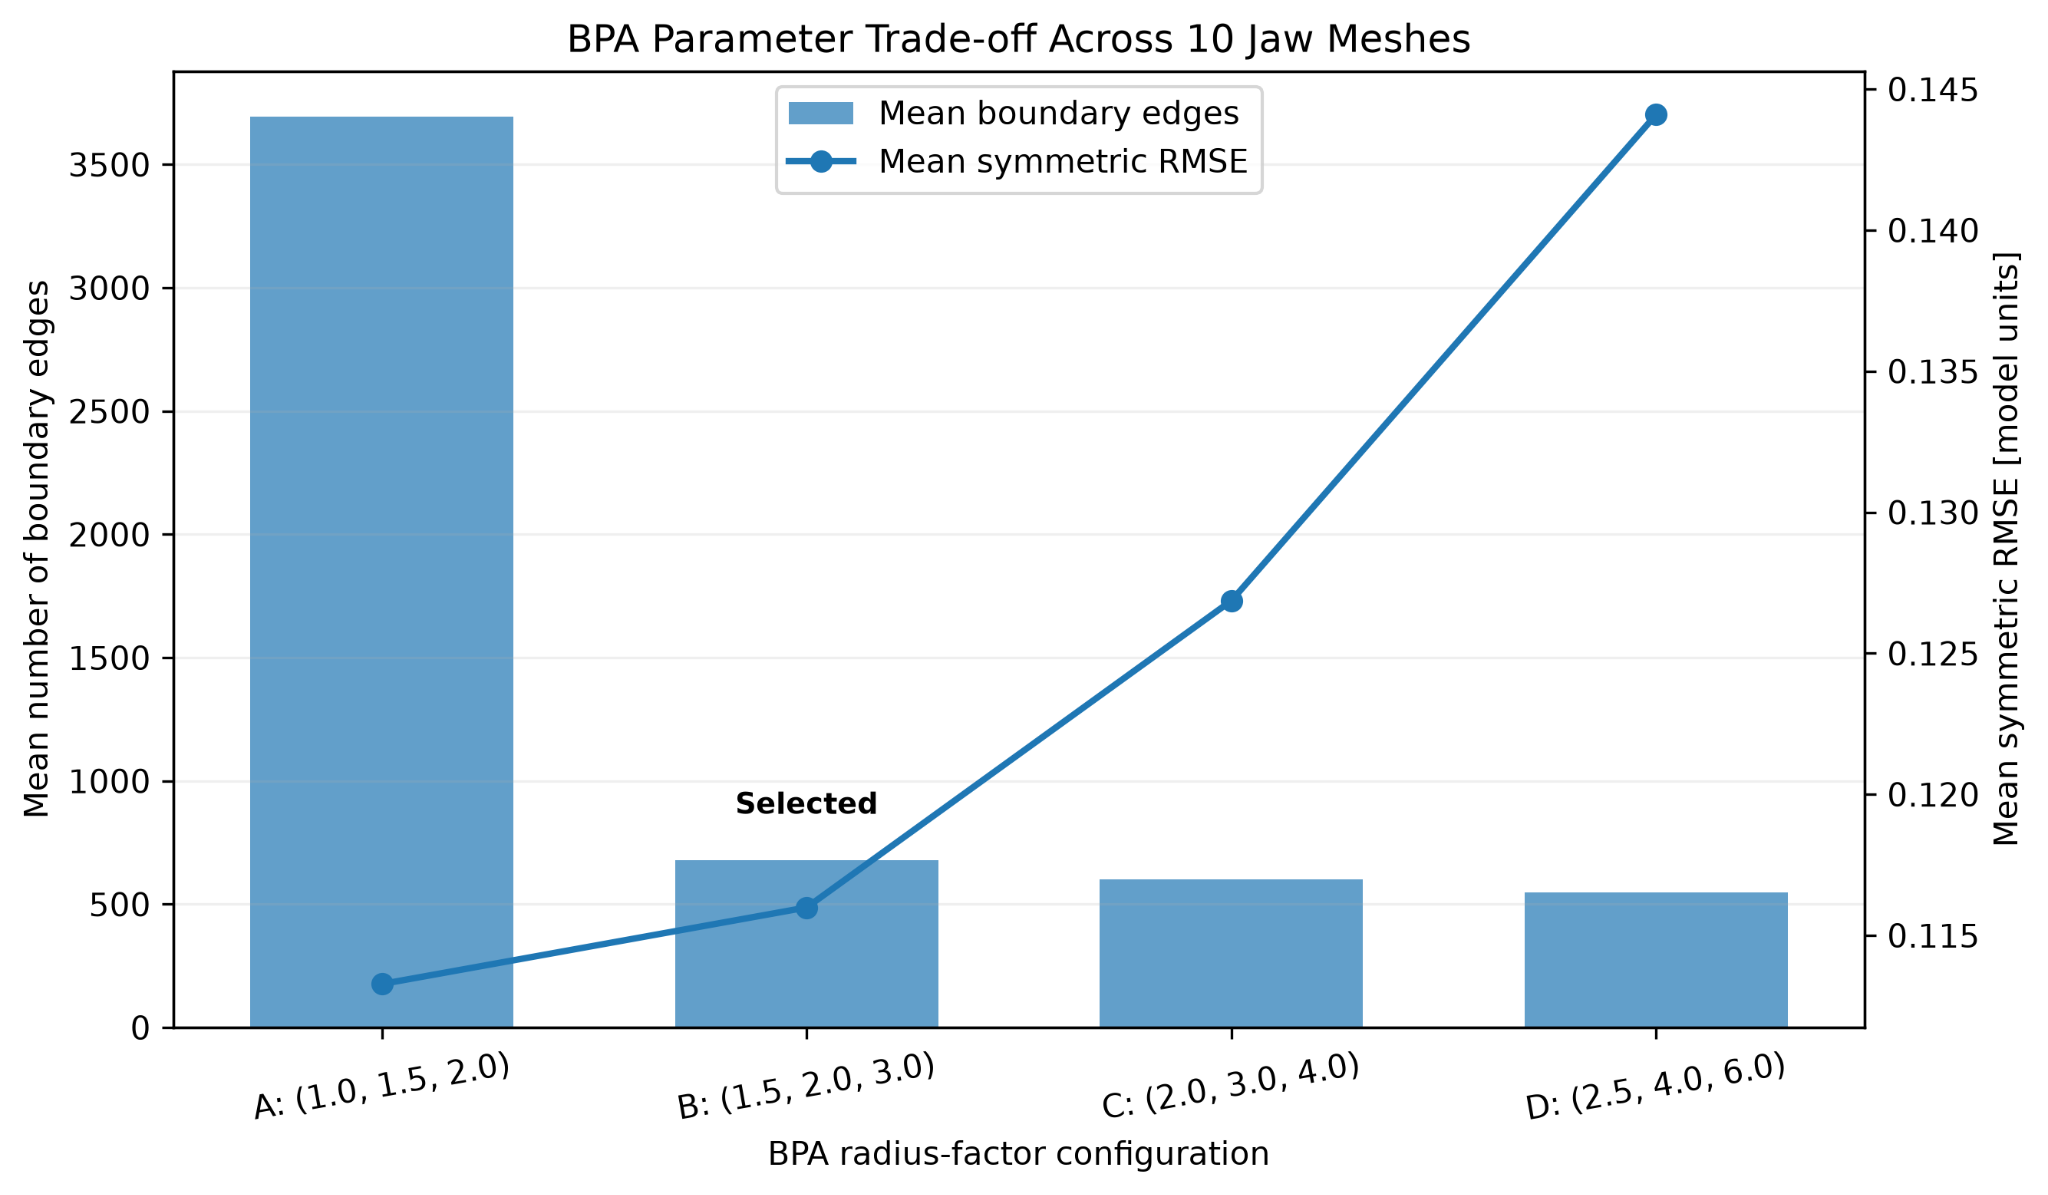
\includegraphics[width=0.84\textwidth]{assets/marvin/model_suite/model_suite_bpa_parameter_tradeoff.png}
    \caption{BPA parameter trade-off across ten jaw meshes. Configuration A minimizes geometric error but leaves many open boundaries. Configuration B is selected as the best compromise between boundary closure and fidelity.}
    \label{fig:model-suite-bpa-tradeoff}
\end{figure*}

\begin{table*}[!t]
\centering
\footnotesize
\setlength{\tabcolsep}{4pt}
\begin{tabular}{lrrrrrr}
\toprule
\textbf{Configuration} & \textbf{Mean sym. RMSE} & \textbf{Mean boundary edges} & \textbf{Mean components} & \textbf{Largest comp. frac.} & \textbf{Mean area ratio} & \textbf{Self-int.} \\
\midrule
A $(1.0,1.5,2.0)$ & \textbf{0.113276} & 3694.1 & 6.0 & 0.998650 & 0.939826 & 0/10 \\
\textbf{B $(1.5,2.0,3.0)$} & 0.115989 & \textbf{678.4} & 3.7 & 0.998970 & \textbf{0.972137} & 0/10 \\
C $(2.0,3.0,4.0)$ & 0.126863 & 600.3 & \textbf{3.2} & \textbf{0.999159} & 0.971531 & 0/10 \\
D $(2.5,4.0,6.0)$ & 0.144096 & 548.1 & 4.3 & 0.998966 & 0.971059 & 0/10 \\
\bottomrule
\end{tabular}
\caption{Aggregate realistic BPA parameter study. Configuration B increases mean symmetric RMSE by only about 2.4\% relative to A while reducing mean boundary edges by about 81.6\%.}
\label{tab:model-suite-bpa-study}
\end{table*}

The same trade-off appears in every model set. Moving from A to B reduces the mean boundary-edge count from 3694.1 to 678.4, while mean symmetric RMSE increases only from 0.113276 to 0.115989. Configurations C and D close only modestly more boundaries than B but increase geometric error by approximately 9.4\% and 24.2\% relative to B. Configuration B is therefore retained as the final realistic BPA setting.

\subsubsection{Poisson versus Final BPA Across Ten Jaws}

Poisson reconstruction and the selected BPA configuration B were then evaluated against all ten original STL surfaces. BPA was more accurate on every model set and produced no self-intersections. Poisson generated fewer open boundaries, but this apparent completeness was achieved by adding large unsupported surface regions.

\begin{table*}[!t]
\centering
\footnotesize
\setlength{\tabcolsep}{4pt}
\begin{tabular}{lrrrrrr}
\toprule
\textbf{Method} & \textbf{Mean sym. RMSE} & \textbf{Median sym. RMSE} & \textbf{Ref.$\rightarrow$Rec. RMSE} & \textbf{Rec.$\rightarrow$Ref. RMSE} & \textbf{Mean area ratio} & \textbf{Self-int.} \\
\midrule
\textbf{BPA} & \textbf{0.115989} & \textbf{0.115584} & \textbf{0.117964} & \textbf{0.113965} & \textbf{0.972137} & \textbf{0/10} \\
Poisson & 1.475913 & 0.999702 & 0.136558 & 2.080730 & 1.414758 & 10/10 \\
\bottomrule
\end{tabular}
\caption{Aggregate surface-reconstruction validation across ten jaw meshes. The large Poisson reconstruction-to-reference error and area ratio reveal unsupported reconstructed surface regions.}
\label{tab:model-suite-poisson-bpa}
\end{table*}

\begin{figure*}[!t]
\centering
\begin{subfigure}[t]{0.48\textwidth}
    \centering
    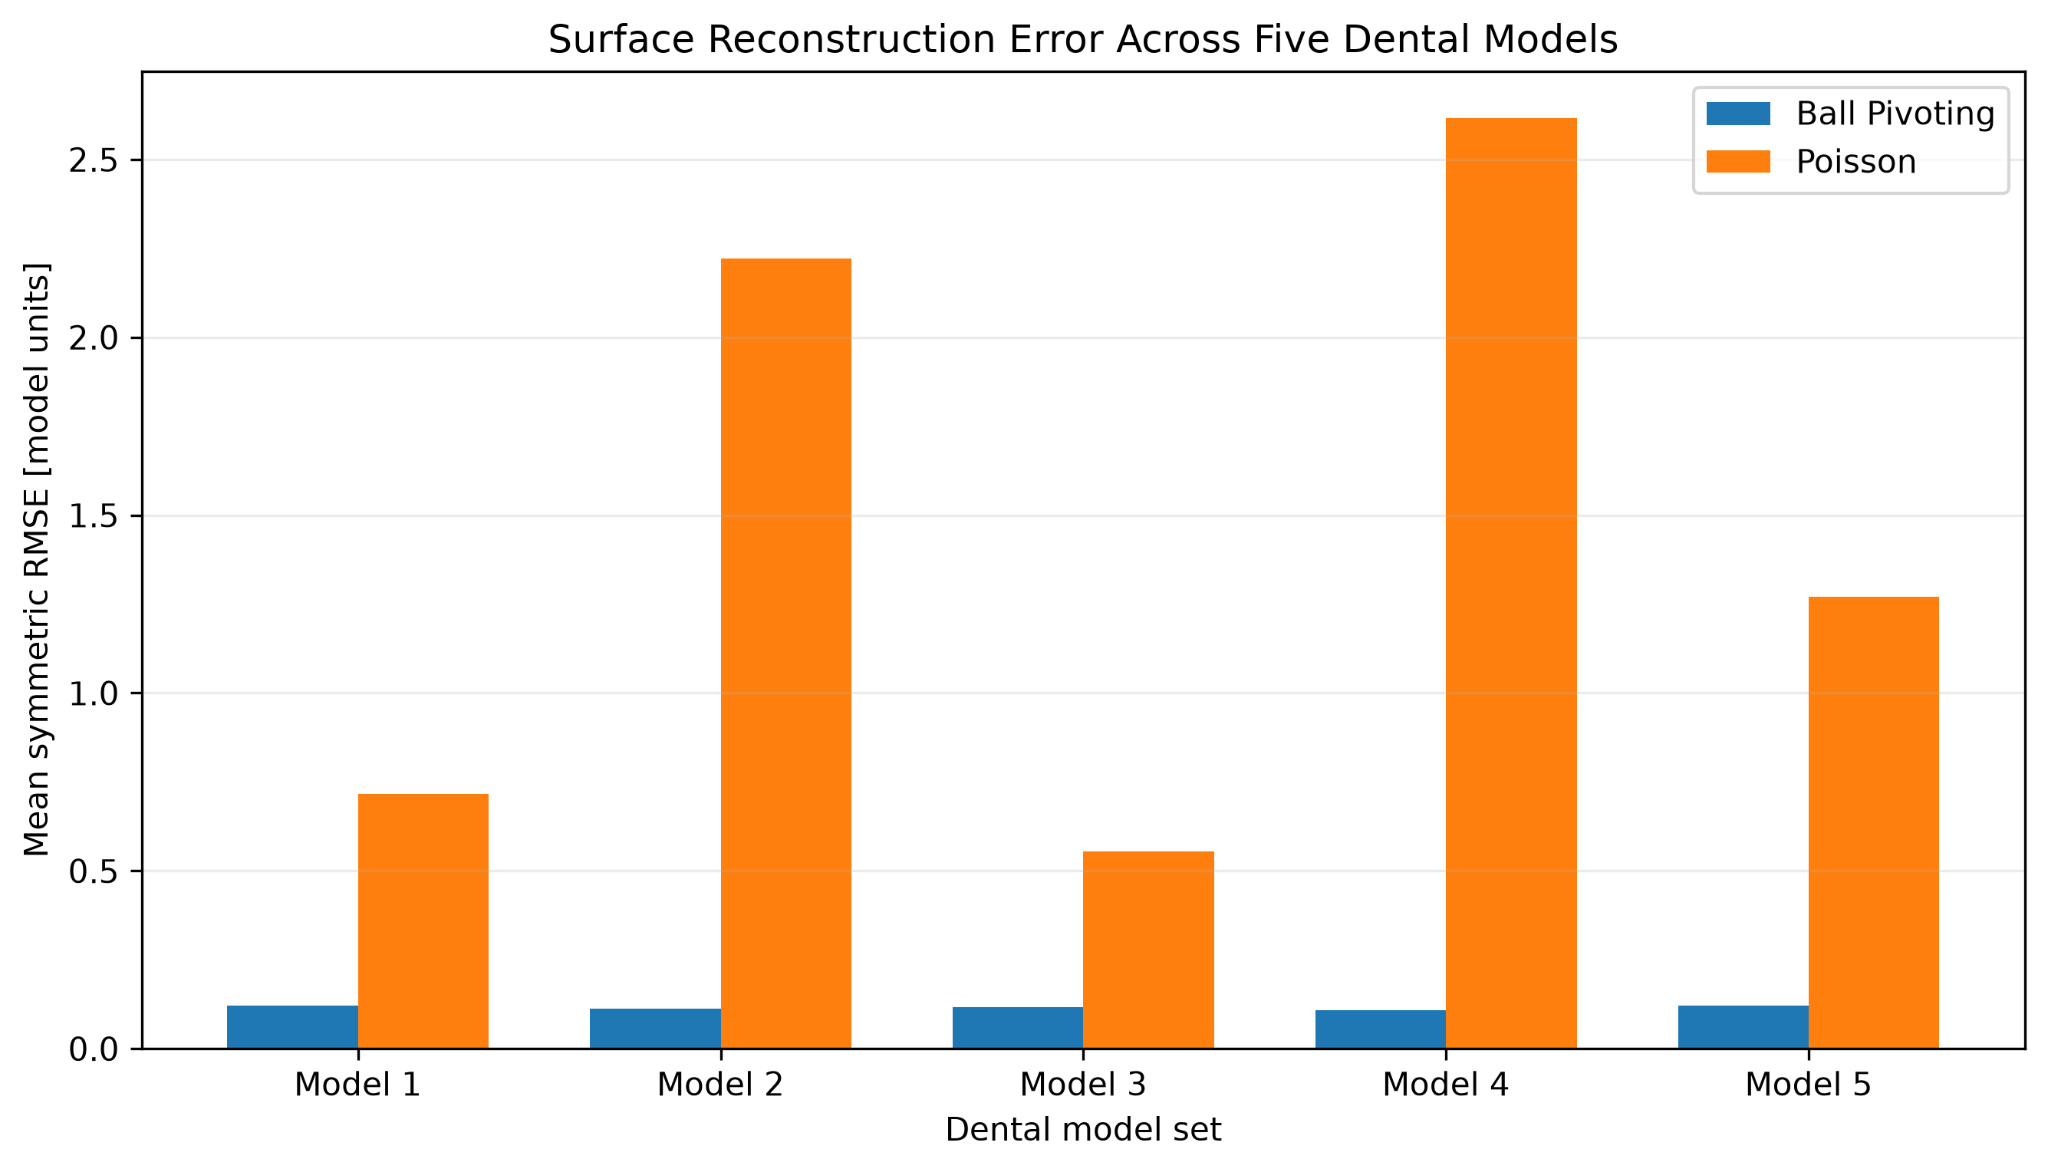
\includegraphics[width=\linewidth]{assets/marvin/model_suite/model_suite_mesh_rmse_by_model.png}
    \caption{Symmetric RMSE by model set.}
\end{subfigure}\hfill
\begin{subfigure}[t]{0.48\textwidth}
    \centering
    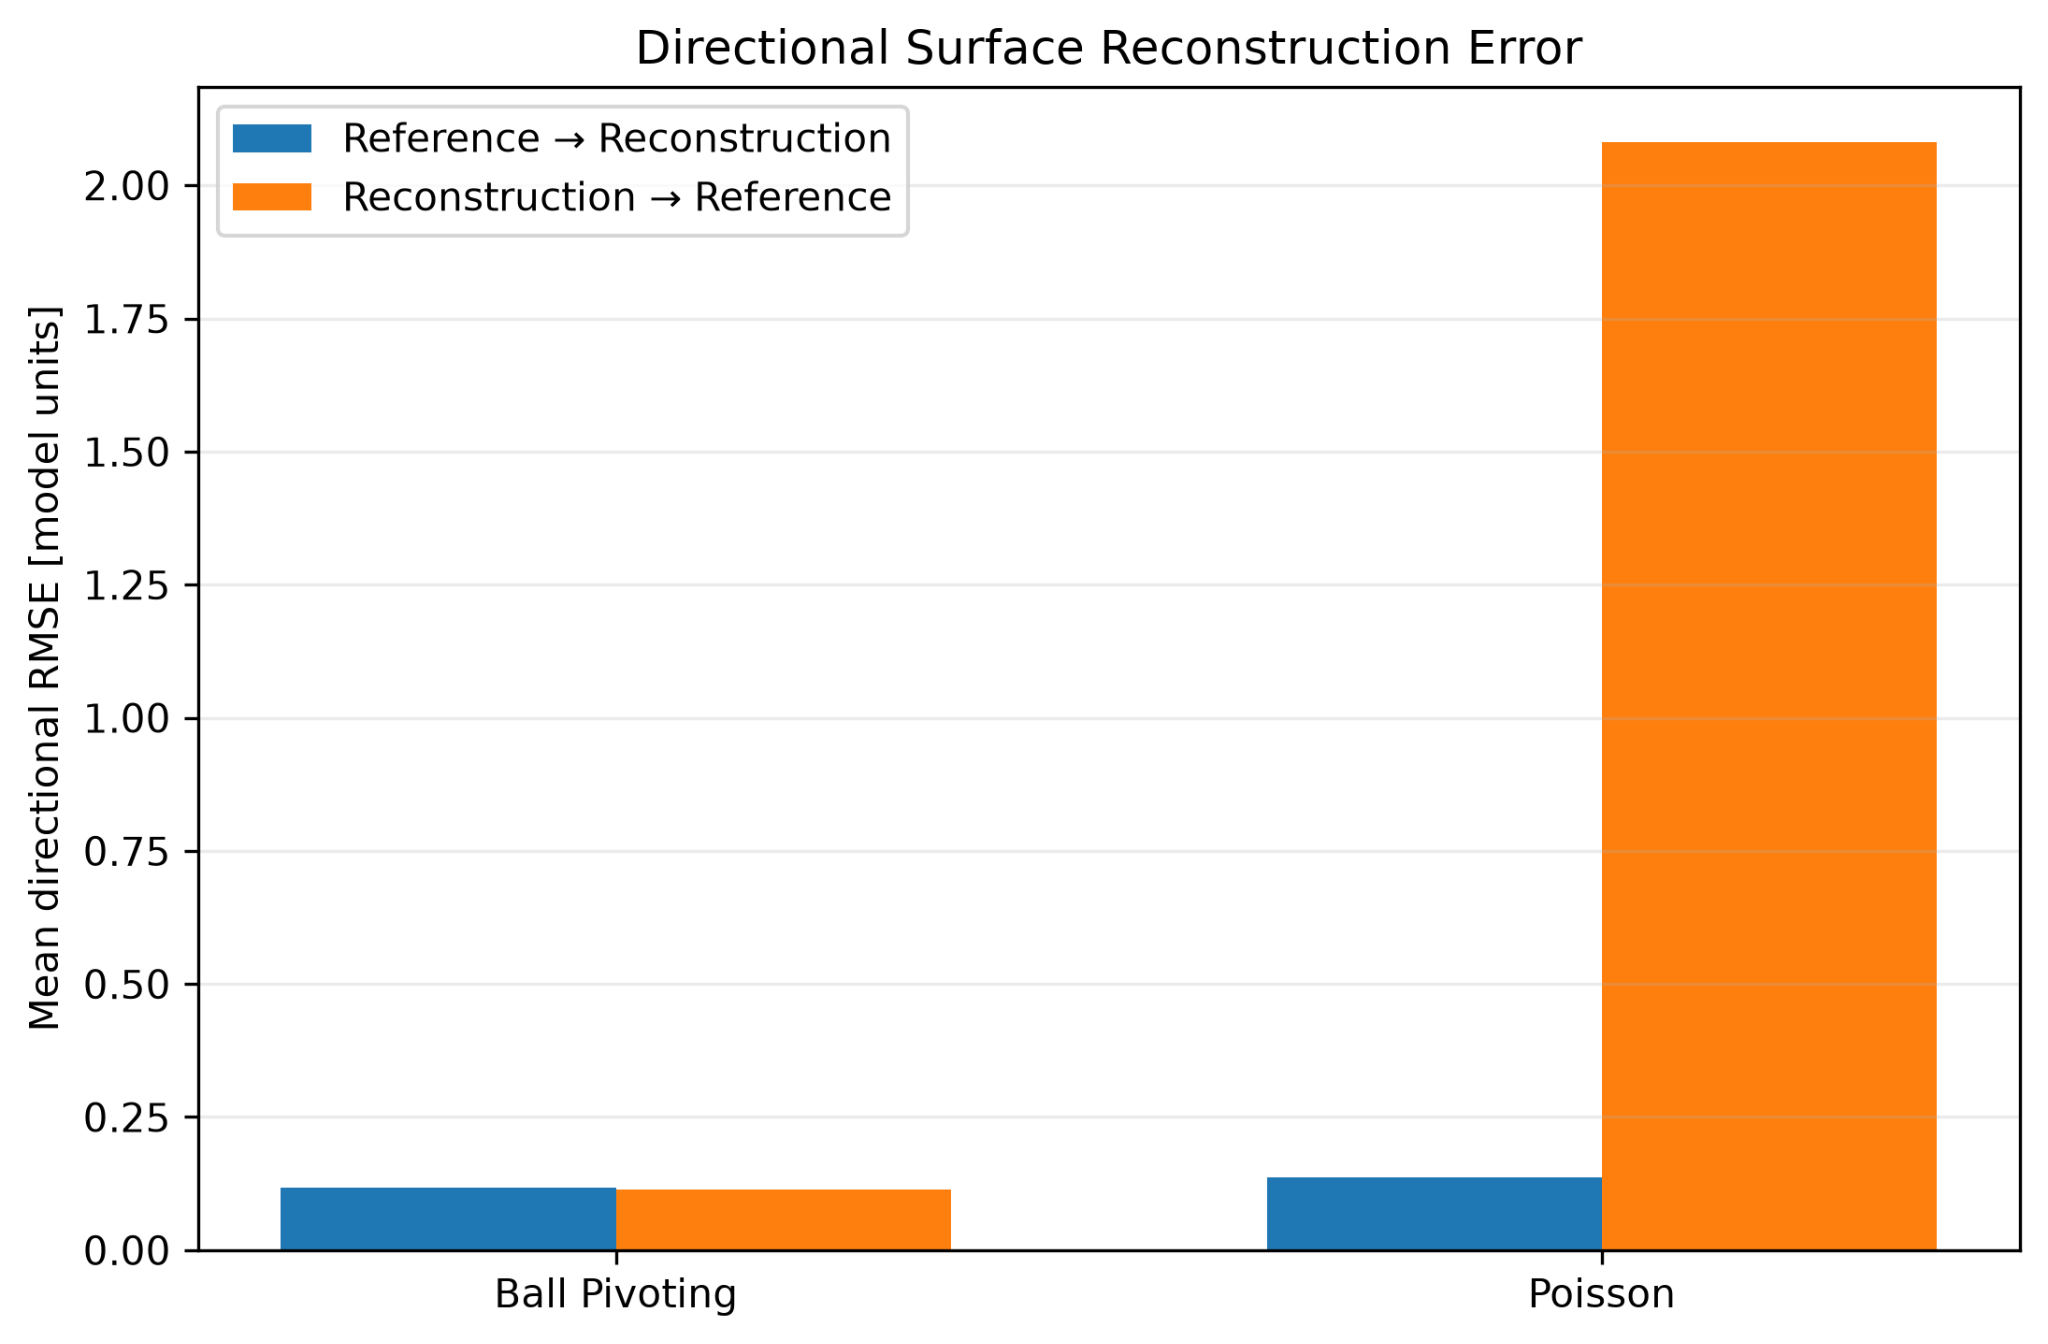
\includegraphics[width=\linewidth]{assets/marvin/model_suite/model_suite_mesh_directional_rmse.png}
    \caption{Mean directional RMSE.}
\end{subfigure}
\caption{Surface-reconstruction generalization across five dental model sets. BPA is consistently more accurate, while Poisson's dominant error occurs in the reconstruction-to-reference direction, indicating unsupported added geometry.}
\label{fig:model-suite-mesh-errors}
\end{figure*}

The directional evaluation is central to this result. Poisson covers much of the reference geometry reasonably well, with a mean reference-to-reconstruction RMSE of 0.1366 model units. In the opposite direction, however, its mean RMSE rises to 2.0807 model units, compared with only 0.1140 for BPA. The mean Poisson surface-area ratio of 1.415 indicates approximately 41.5\% more reconstructed area than the reference on average, whereas BPA remains close to the reference at 0.972. All ten Poisson meshes contain self-intersections; none of the ten BPA meshes do.

\begin{figure*}[!t]
\centering
\begin{subfigure}[t]{0.48\textwidth}
    \centering
    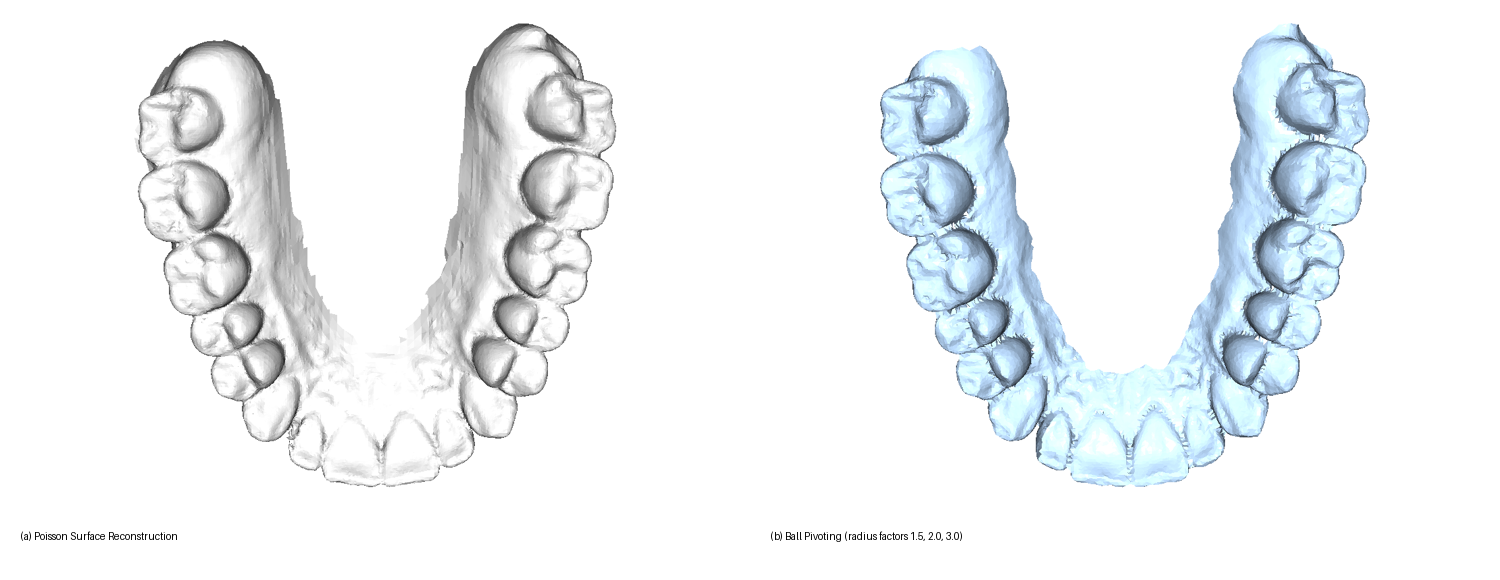
\includegraphics[width=\linewidth]{assets/marvin/realistic_poisson_vs_bpa.png}
    \caption{Representative upper-jaw comparison.}
\end{subfigure}\hfill
\begin{subfigure}[t]{0.48\textwidth}
    \centering
    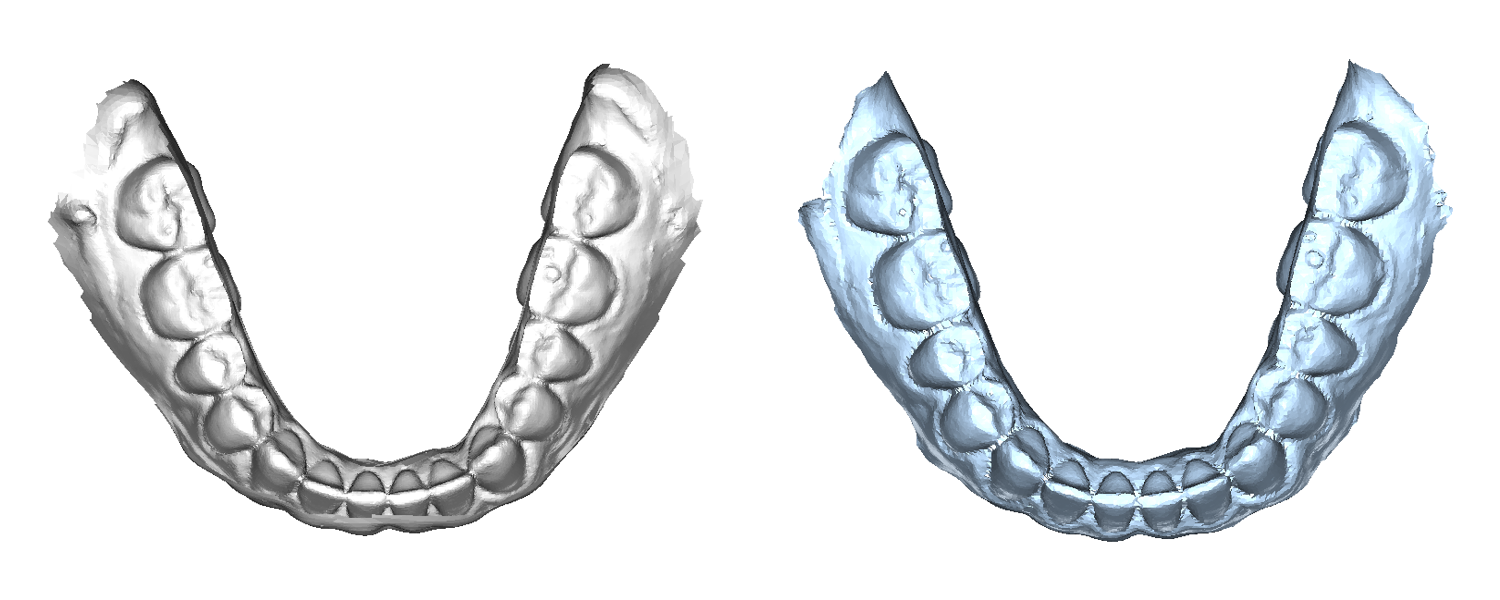
\includegraphics[width=\linewidth]{assets/marvin/lower/lower_05_poisson_vs_bpa.png}
    \caption{Representative lower-jaw comparison.}
\end{subfigure}
\caption{Representative qualitative comparison from Model~1. Poisson appears smooth and closed, but the ten-jaw quantitative evaluation shows substantially larger unsupported surface error than BPA.}
\label{fig:representative-poisson-bpa}
\end{figure*}

The final realistic reconstruction choice is therefore:
\begin{center}
\textbf{Ball Pivoting with radius factors $(1.5,2.0,3.0)$.}
\end{center}

\subsection{Discussion: Synthetic Screening versus Realistic Validation}
\label{sec:marvin-discussion}

The two-stage evaluation shows why broad synthetic screening and multi-model realistic validation serve different purposes. The synthetic generator isolates overlap, rotation, translation, and noise, which makes failure modes interpretable. The five-model suite then tests whether those conclusions survive substantial changes in actual dental geometry. The second stage both revised and strengthened the provisional choices: RANSAC replaced FGR as the final global registration method, while BPA was confirmed and its realistic radius configuration changed from A to B.

\begin{table*}[!t]
\centering
\footnotesize
\begin{tabularx}{\textwidth}{@{}lYYY@{}}
\toprule
\textbf{Decision} & \textbf{Synthetic evidence} & \textbf{Five-model realistic evidence} & \textbf{Final interpretation} \\
\midrule
Global registration & FGR offered a strong accuracy/runtime compromise in the controlled benchmark & RANSAC solved all 30 zero-noise adjacent pairs and stayed at 100\% through $\sigma=0.10$ & Select RANSAC + ICP for robustness \\
Multiway chaining & Small error in four-fragment synthetic baseline & Maximum global error across 30 non-reference poses: 0.008239 model units and $0.02266^\circ$ & Sequential four-fragment accumulation remains small \\
Surface reconstruction & BPA strongly outperformed Poisson in bidirectional error & BPA outperformed Poisson on every model set; 0/10 versus 10/10 self-intersecting meshes & Retain BPA \\
BPA radii & Configuration A minimized synthetic RMSE & B reduced boundary edges by 81.6\% versus A for only 2.4\% higher mean RMSE & Use configuration B on realistic dental geometry \\
\bottomrule
\end{tabularx}
\caption{How five-model validation revised or confirmed the provisional synthetic conclusions.}
\label{tab:synthetic-vs-realistic-discussion}
\end{table*}

A second lesson concerns metric choice. FGR often has excellent median transform errors despite catastrophic failures, so median precision alone would hide robustness problems. Likewise, Poisson can look visually smooth and has relatively few boundary edges, yet its reconstruction-to-reference error and inflated surface area reveal unsupported geometry. The final decisions therefore combine transform error, success rate, bidirectional surface distance, boundary structure, connected components, surface-area ratio, and self-intersection tests rather than relying on a single metric.

\subsection{Reproducibility and Integration into the Shared Pipeline}
\label{sec:marvin-reproducibility}

All experiments are deterministic where possible. The synthetic stress tests use 10 repetitions per condition with controlled dataset-seed ranges and reproducible algorithm seeds; the same repetition index is reused across values within a stress-test series so that the intended parameter change dominates the comparison. Open3D seed 42 is used for surface sampling. The five-model zero-noise benchmark assigns deterministic algorithm seeds to every model/jaw/pair combination. In the noise experiment, deterministic per-model, per-jaw, per-level, and per-repetition seeds generate the noisy clouds, and every algorithm receives the same perturbed geometry. Intermediate outputs are stored as PLY meshes/point clouds and CSV or NumPy files containing metrics and poses.

The module boundaries also define the hand-off to the surrounding DentaVision project. The image-acquisition and 3-D reconstruction stage provides point-cloud fragments. The present registration stage aligns these fragments and exports a merged point cloud. Surface reconstruction then produces an explicit mesh suitable for downstream visualization or later processing. Generated test fragments and intermediate outputs can be reproduced from the source STL models and are therefore not required to be versioned in the shared repository.


For the final repository organization, reusable implementation code remains under \texttt{src/registration3d}, while executable studies are grouped under a top-level \texttt{experiments/} directory. Report-figure generation and diagnostic utilities are kept separately in \texttt{visualization/} and \texttt{diagnostics/}. Historical single-model experiment drivers are archived rather than mixed with the final five-model study. This organization keeps the core package importable while making the experimental provenance of the reported numbers explicit. The principal five-model drivers are the pairwise benchmark, noise benchmark, sequential multiway benchmark, BPA parameter study, and BPA-versus-Poisson mesh validation.


\begin{table}[!t]
\centering
\scriptsize
\setlength{\tabcolsep}{3pt}
\begin{tabularx}{\columnwidth}{@{}lY@{}}
\toprule
\textbf{Experiment driver} & \textbf{Purpose} \\
\midrule
\texttt{realistic\_model\_suite\_pairwise\_benchmark.py} & Five-algorithm comparison on 30 adjacent fragment pairs \\
\texttt{realistic\_model\_suite\_noise\_benchmark.py} & Shared-noise robustness evaluation over 2,400 registrations \\
\texttt{realistic\_model\_suite\_multiway\_ransac.py} & Sequential four-fragment RANSAC multiway evaluation \\
\texttt{realistic\_model\_suite\_bpa\_parameter\_study.py} & BPA radius trade-off across ten jaws \\
\texttt{realistic\_model\_suite\_mesh\_validation.py} & Final BPA-versus-Poisson surface comparison \\
\bottomrule
\end{tabularx}
\caption{Principal final experiment drivers after repository cleanup. All are executed from the project root through the Poetry environment.}
\label{tab:experiment-drivers}
\end{table}

\begin{table}[!t]
\centering
\footnotesize
\begin{tabularx}{\columnwidth}{@{}lY@{}}
\toprule
\textbf{Artifact} & \textbf{Role in pipeline} \\
\midrule
Fragment PLY files & Pairwise and multiway registration input \\
Estimated pose arrays & Reproducible multiway transformation state \\
Merged point cloud & Interface between registration and mesh reconstruction \\
Evaluation CSV/JSON & Quantitative experiment results \\
Final PLY mesh & Indexed geometry for processing and visualization \\
Final STL mesh & Interoperable triangular surface export \\
\bottomrule
\end{tabularx}
\caption{Principal artifacts exchanged or exported by the registration/model-construction stage.}
\label{tab:pipeline-artifacts}
\end{table}

\subsection{Final Method Selection and Limitations}
\label{sec:marvin-final-selection}

The final method selection differs from the provisional synthetic choice because the realistic validation exposed failure modes that were not sufficiently represented by the first synthetic benchmark.

\begin{table}[H]
\centering
\scriptsize
\setlength{\tabcolsep}{2.5pt}
\begin{tabularx}{\columnwidth}{@{}lYY@{}}
\toprule
\textbf{Stage} & \textbf{Final choice} & \textbf{Key evidence} \\
\midrule
Pairwise & \textbf{FPFH + RANSAC + P2Plane ICP} & 30/30 zero-noise successes; strongest noise robustness \\
Multiway & \textbf{Sequential four-fragment chaining} & Explicit pairwise-error accumulation without loop-closure correction \\
Surface & \textbf{Ball Pivoting} & Lower bidirectional error; 0/10 self-intersecting meshes \\
BPA radii & \textbf{$(1.5,2.0,3.0)$} & 81.6\% fewer boundary edges than A for 2.4\% higher mean RMSE \\
Simplification & \textbf{$\approx$30k triangles} & 25.04\% triangle reduction for 0.171\% RMSE increase in synthetic study \\
\bottomrule
\end{tabularx}
\caption{Final design decisions after synthetic screening and five-model realistic validation.}
\label{tab:final-selection}
\end{table}

\subsubsection{Threats to Validity}

\paragraph{Internal validity.}
The experiments were designed to make algorithmic differences dominate over incidental randomness. All methods within one noisy trial receive exactly the same perturbed point clouds, dataset and algorithm seeds are deterministic, and pairwise transformations can be evaluated against exact virtual ground truth. Nevertheless, stochastic global registration can still exhibit seed-dependent outcomes. The reported benchmark therefore characterizes the implemented configuration and seed-controlled protocol rather than every possible random realization. The Wilson intervals shown for RANSAC visualize finite-sample uncertainty only; the three nonzero-noise repetitions share the same 30 base fragment pairs and are not treated as 90 independent dental geometries.

\paragraph{Construct validity.}
Correctness is operationalized by transform error when ground truth is available, using thresholds of one model unit and one degree in the realistic registration study. These thresholds are deliberately more informative than fitness or inlier RMSE alone, because repetitive dental surfaces can support plausible but incorrect correspondence sets. Surface quality is likewise assessed bidirectionally instead of relying only on appearance or watertightness. However, the mesh-distance evaluation is sampling based and therefore approximates, rather than exactly computes, point-to-triangle surface distance. In addition, STL does not encode physical units, so absolute distances are reported in model units and should not be interpreted as millimeters without verified source metadata.

\paragraph{External validity.}
The five realistic model sets are STL surfaces that are sampled and fragmented in software; they are substantially more diverse than the synthetic dental-like generator but are not actual intraoral scanner captures. Real acquisitions may contain occlusions, outliers, strongly nonuniform point density, reflections, motion artifacts, and scanner-specific systematic error. The added perturbation is isotropic Gaussian positional noise rather than a calibrated sensor-noise model. Furthermore, the ten jaws have intentionally similar overall scale and do not systematically cover severe malocclusions, missing teeth, restorations, pathological anatomy, or deliberately varied acquisition conditions. Generalization to those clinically relevant geometry classes therefore remains untested. Finally, the realistic multiway experiment evaluates four-fragment sequential chaining without loop closures; substantially longer acquisition trajectories may require pose-graph optimization and explicit loop-consistency checks.

\FloatBarrier
\subsection{Conclusion}
\label{sec:marvin-conclusion}

A complete registration and model-construction pipeline was implemented and evaluated from multiple dental point-cloud fragments to reconstructed triangular surfaces. Five pairwise registration algorithms were first compared under controlled synthetic changes in overlap, rotation, translation, and noise. The synthetic benchmark initially favored FPFH + FGR + Point-to-Plane ICP, but the subsequent five-model validation exposed catastrophic FGR outliers and changed the final selection to FPFH + RANSAC + Point-to-Plane ICP.

Across five distinct dental model sets comprising ten jaw meshes and 30 adjacent zero-noise fragment pairs, the selected RANSAC pipeline achieved 30/30 successful registrations with mean translation and rotation errors of 0.001921 model units and $0.00948^\circ$. Under added Gaussian positional noise it maintained 100\% observed success through $\sigma=0.10$ and achieved 84.44\% at $\sigma=0.20$. Sequential four-fragment multiway registration across all ten jaws yielded a maximum global pose error of only 0.008239 model units and $0.02266^\circ$.

For surface reconstruction, BPA configuration B $(1.5,2.0,3.0)$ provided the best realistic trade-off between geometric fidelity and boundary closure. Across all ten jaw meshes, BPA achieved a mean symmetric RMSE of 0.115989 compared with 1.475913 for Poisson. Poisson's mean reconstruction-to-reference RMSE reached 2.080730 and its mean area ratio 1.414758, indicating substantial unsupported geometry; all ten Poisson meshes contained self-intersections, whereas none of the BPA meshes did.

The main outcome is therefore not only a final algorithm choice but a reproducible selection strategy: controlled synthetic experiments expose specific failure modes, while multi-model realistic geometry determines which methods generalize sufficiently well to be carried forward into the DentaVision pipeline.

\chapterbreak

\section{title}
\sectionauthors{Irmak Damla Özdemir}
\section{Introduction}
DentaVision Control Panel is a Graphical User Interface, that Intraoral Scanning sureci boyunca end user ile interact etmeye araci olan conceptual(burda bu ui robot simulasyonu ile henuz bagli olmadigi ve gelecek Implementationlarda belki yapilabilecegi icin conceptual demek istedim yanlissa alternatif bi kelime bul) bir aractir.  


\subsection{Purpose}
 Proje kapsaminda saglik personeli tarafindan kullanilmak uzere bir graphical user interface gelistirilmeye karar verildi. 
 Bu arayuzun ana amaci, scanning sirasinda moderation yapacak personele uygun graphical destek saglamak ve oral scanning yapilacak hastanin guvenligi icin kafasinin sabit oldugunu kontrol eden bir sistem implemente etmek.
 Bu sistem, automation kapsaminda computer vision (bu terimin buraya uygunlugundan emin degilim kontrol et gerekirse alternatif bul) kullanilarak hastanin dis arkinin olculerini estimate ederek robotun ilerleyecegi konumu belirlemeyi denerken asamaya ozel komut butonlariyla sureci daha guvenli kilmaya calisir. 
 Bunun yani sira, GUI'Da robot pozisyonlarinda manuel adjustmentlar yapilabilmesini saglayan bir panel ile gerektigi durumlarda saglik personeline yetki verilerek anpassung yapilabilmesini ongorur.    

\subsection{Scope}

Control Panel gelecek implementationda/ bir sonraki adimda roboter arm trajeksiyon logici ile birlestirelerek kullanilmasina yonelik conceptual oalrak gelistirilmistir. (bu cumle inverse kinematics ile desteklenebilir mi ?)
DentaVision, bir dental tarama işlemi sırasında hastanın kafa pozisyonunu kamera üzerinden gerçek zamanlı olarak takip eden ve operatörün seçtiği dişe göre bir robot kolun ulaşması gereken hedef koordinatları (X, Y, Z, RX, RY, RZ) hesaplayan bir kontrol panelidir. Sistem; MediaPipe Face Mesh ile yüz ve ağız tespiti yapmakta, ağzın kameradaki referans noktasına göre konumunu ve oryantasyonunu 2D landmark verilerinden kestirmekte, seçilen dişin sabit anatomik ofsetini bu kafa pozisyonuna ekleyerek Tooth Target'ı üretmekte ve Start → Scan → Pause olarak tanımlanan dört fazlı bir iş akışıyla operatörü yönlendirmektedir. Buna ek olarak, Joint Control panelinden yapılan manuel jog hareketleri, bu hesaplanan hedef baz alınarak (baseline) terminale yazdırılmaktadır.

Projenin kapsamı, yazılım ve algoritma seviyesindeki bu hesaplama ve kullanıcı arayüzü mantığıyla sınırlıdır; gerçek bir robot kol donanımına bağlantı içermemekte, hesaplanan eklem değerleri yalnızca terminale yazdırılmaktadır. Kafa pozisyonu kestirimi, cv2.solvePnP tabanlı gerçek bir 3D poz kestirimi ya da kamera iç/dış kalibrasyon matrisi kullanmamakta; bunun yerine basitleştirilmiş bir 2D landmark geometrisine dayanmaktadır. Benzer şekilde, diş hedefi hesaplamasında kullanılan diş yayı (dental arch) modeli hastaya özel bir ölçümden değil, sabit ve genel bir geometrik şablondan türetilmektedir. Sistem, hastanın muayene boyunca sabit bir koltuk ve headrest düzeninde, kameraya sabit bir mesafede konumlandığını varsaymakta; bu nedenle piksel–gerçek dünya dönüşümü, tek bir sabit mesafe için kalibre edilen bir ölçekleme sabiti ile yapılmaktadır.
\subsection{Terminology}

\subsubsection{FDI Tooth Numbering}
\subsubsection{XYZ RX RY RZ}


\section{System Overview}


\subsection{Arhitecture}
DentaVision is organized as a processing pipeline that turns a
live camera feed into an absolute Tooth Target position. At
every frame, the system moves through four stages: \textbf{camera input
acquisition}, \textbf{facial and mouth detection}, \textbf{geometric
computation}, and \textbf{panel display}. Each stage is implemented as a
separate module with a single responsibility, so that the
detection logic knows nothing about robot motion, and the display layer
knows nothing about how a coordinate was derived. Figure~\ref{fig:overview}
summarizes this flow:

\begin{figure}[ht]
    \centering
    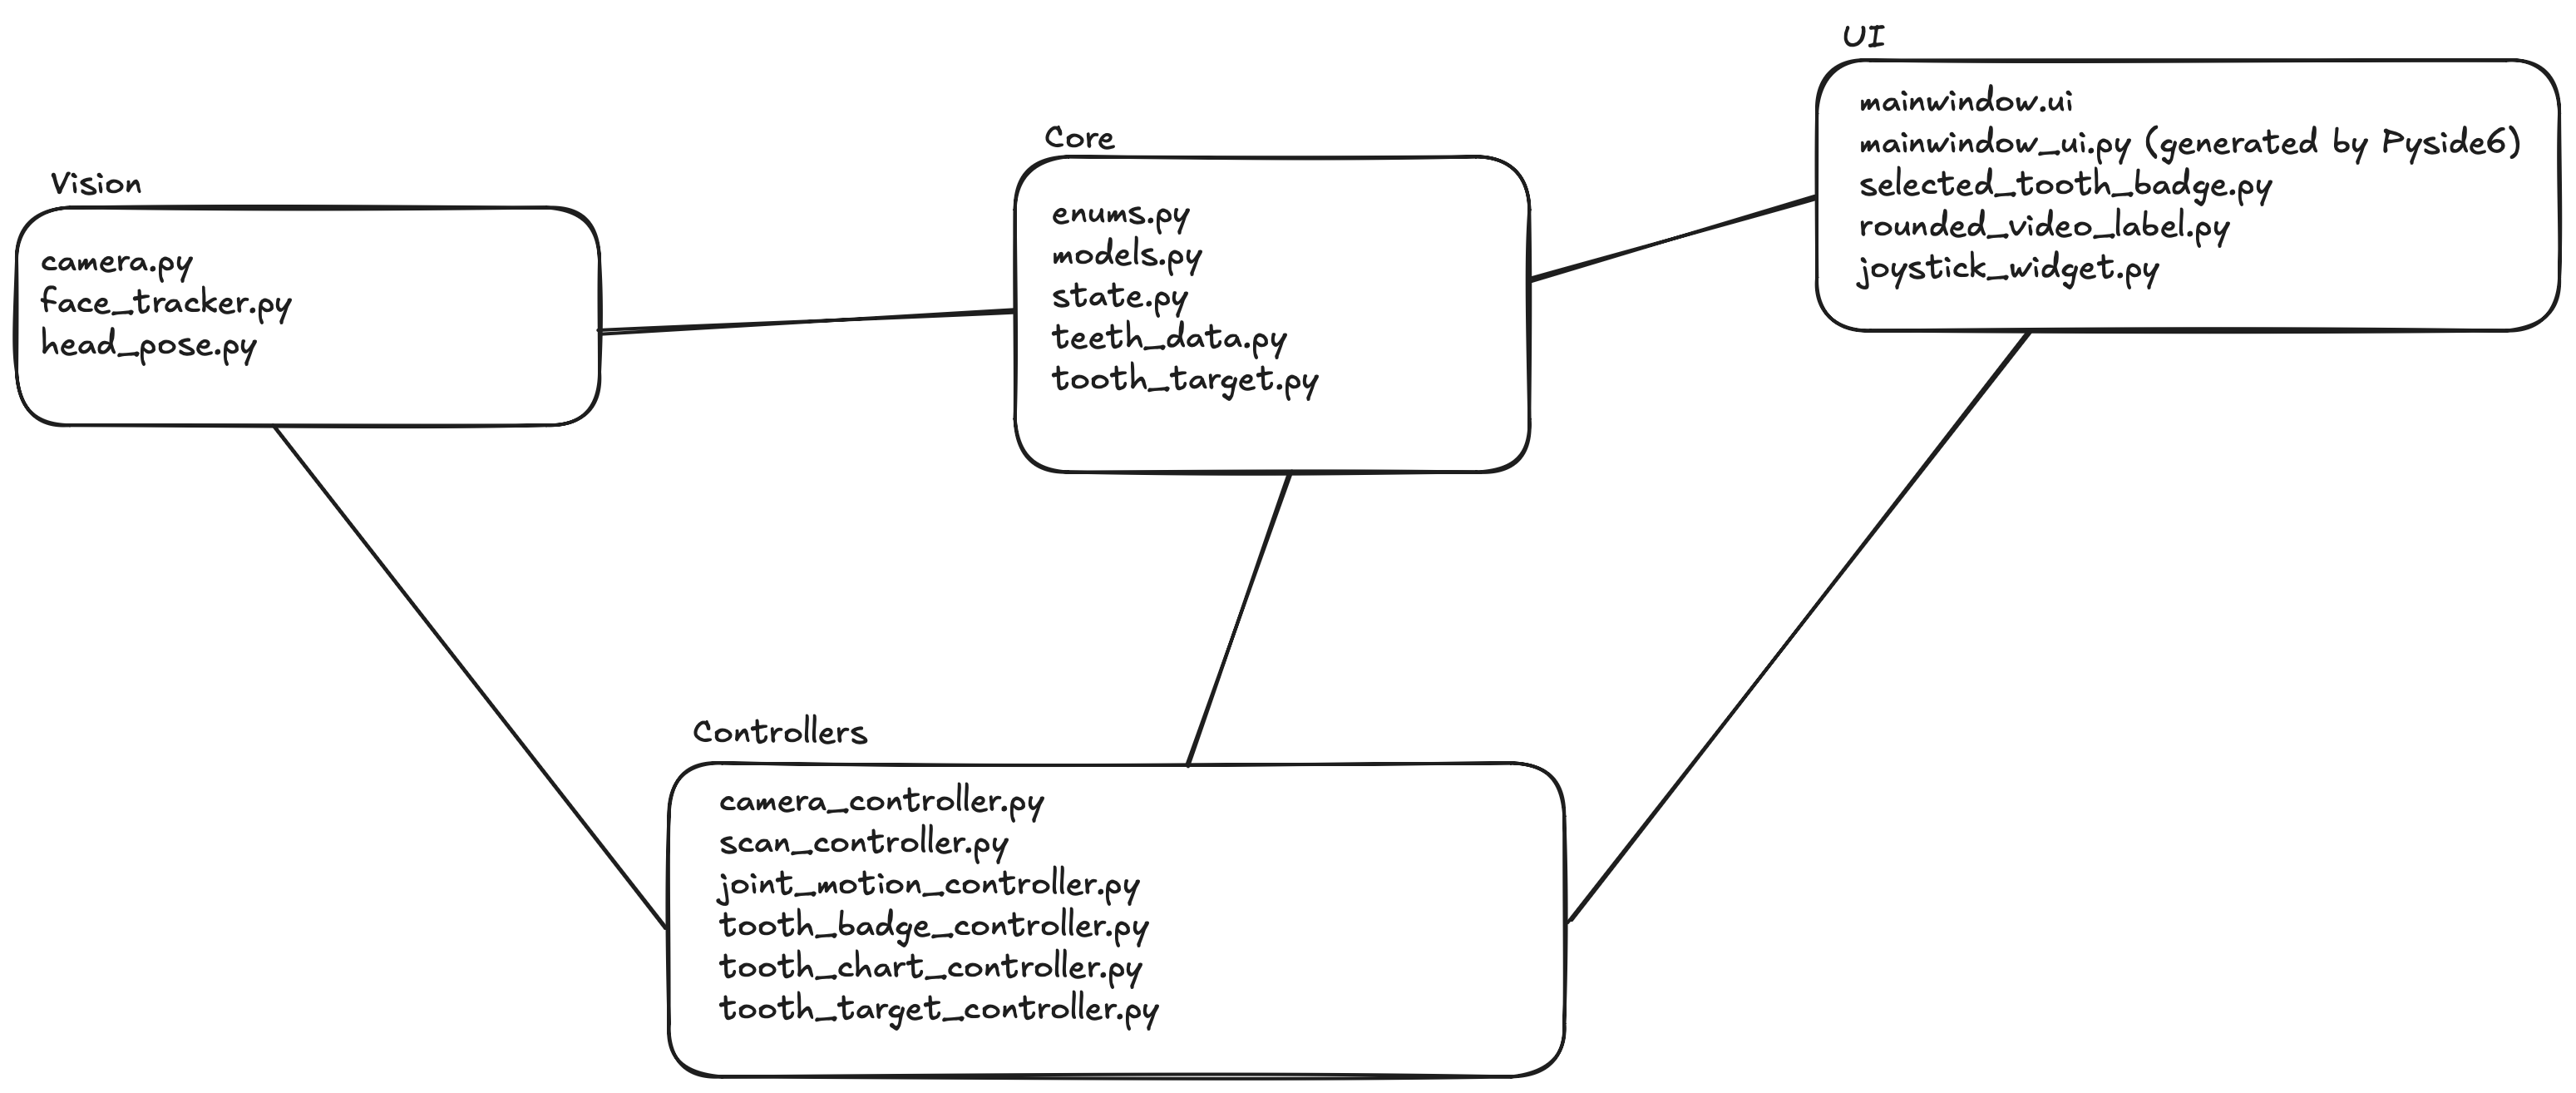
\includegraphics[width=1.1\columnwidth]{ui_assets/overview.png}
    \caption{System Organization Overview drawn in Excalidraw}
    \label{fig:overview}
\end{figure}


\subsection{Data Flow}



\subsection{Dependencies and System Requirements}

The panel logici python ve design qt araciligiyla gelistirildi. Panelde bulunan kamera ve face detection icin OpenCV ve MediaPipe gibi python computer vision kutuphaneleri kullanildi. 
Baslica kullanilan componentleri Tablo~\ref{tab:dependencies}de gorulmektedir.    


\begin{table}[h]
    \centering
    \caption{Dependencies and Development Tools Used in Control Panel}
    \label{tab:dependencies}
    \begin{tabularx}{\columnwidth}{@{}l X@{}}
        \toprule
        \textbf{Component} & \textbf{Purpose} \\
        \midrule
        Python   & Used to implement the application \\
        PySide6 & GUI framework (Qt for Python bindings) \\
        MediaPipe & Face and mouth landmark detection \\
        OpenCV & Camera capture, color conversion, and overlay drawing \\
        Qt Creator & Visual design and layout editing of UI \\
        \bottomrule
    \end{tabularx}
\end{table}

\subsection{Operating Environment and Physical Setup Assumptions}
DentaVision Control Panelin dogru calismasi icin varsayilan fiziksel bir kurulum bulunmaktadir:

\begin{itemize}
    \item Control Paneli touchable bir screen olarak dusunulmustur ve saglik personeli bu paneldeki componentleri dokunmatik olarak kullanir/kontrol eder.
    \item Calisan bir webcam veya USB kamera gereklidir, Mediapipe CPU uzerinde de calisabildiginden GPU gerekli degildir. (bu bilgi gerekli mi?) 
    \item Patient klinikte bulunan sabit bir dental koltukta, kafasi dental head stabilizer ile sabitlenmis bir sekilde oturur. Muayene boyunca kafa poziyosnu fix kalir, asagi yukari veya saga sola hareket etmez.
    \item Koltugun yuksekligi ve kameraya olan mesafesi visionun guvenilirligini etkilemeyecek bir mesafede ayarlanir ve sabit kabul edilir.
    \item Panelde görülen kamera bir konuma sabit monte edilir ve hareket etmez.
    \item Kamera ve Kontrol Panel ayni cihazda bulunabilirken, hasta koltuguna entegre edilen external bir kamera da kullanilabilir.
    \item Odadaki isiklandirma kamera gorus acisi icin optime edilir veya kameranin gordugu alana manuel bir isik eklenmelidir.
\end{itemize}

Bu setuplar ile kamera ve hasta arasi hep sabit bir mesafede oldugu icin HeadPosition.z degeri kameradan olculmez, sabit bir baseline degeri olarak alinir. 
Ayni zamanda, bu sabit olcum sayesinde kameradaki bir pixelin kac cme denk geldigini ifade eden CM\_PER\_PIXEL kalibrasyon sabiti tek bir ölcümle belirlenebilir ve tooth targetin hastanin agiz boyutuna daha uyumlu calismasi hedeflenmektedir.
Koltuk veya kamera yeri degisirse yeniden kalibrasyon gerekmektedir. 

\section{User Interface Design}
Control panel UI Designinda MEdical ortama ve personal user experiencei icin user flow Figure~\ref{fig:userflow} dusunulup olabildigince optimal bir sekilde gerceklestirilmeye calisilmistir. 


\begin{figure}[t]
    \centering
    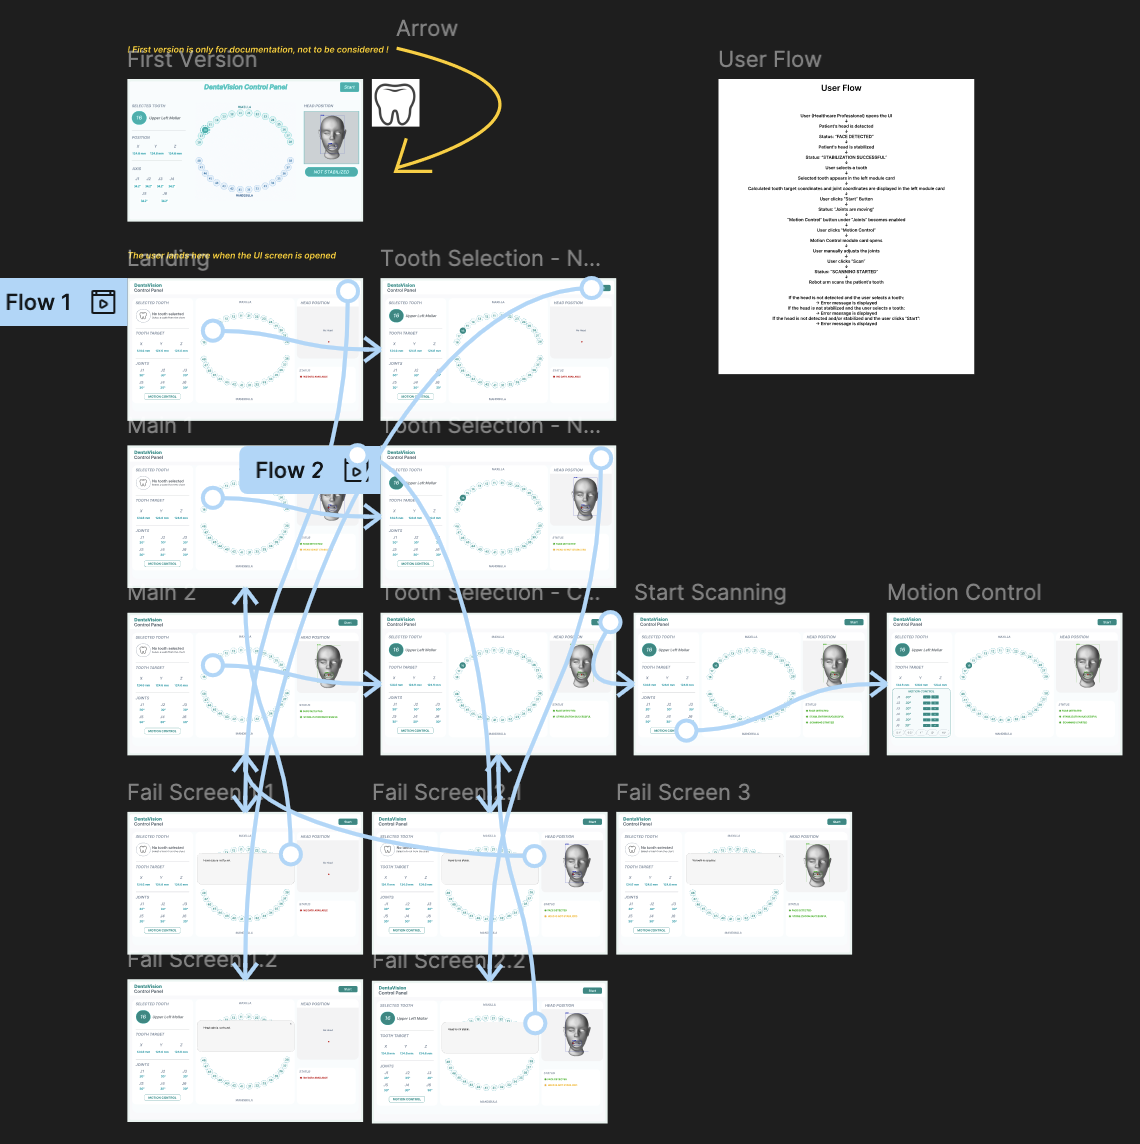
\includegraphics[width=\columnwidth,height=0.45\textheight,keepaspectratio]{ui_assets/figma_.png}
    \caption{Figma Control Panel UI Design Layout}
    \label{fig:userflow}
\end{figure}

Baslangicta daha basit bir user flow baz alinarak Figma da design ilk versiyonu Figure ~\ref{fig:figma} olusturulmustur ve sonrasinda iterasyonla bu dizayn iyilestirilip implementasyon asamasinda optimize edilmeye devam edilmistir.

\begin{figure}[t]
    \centering
    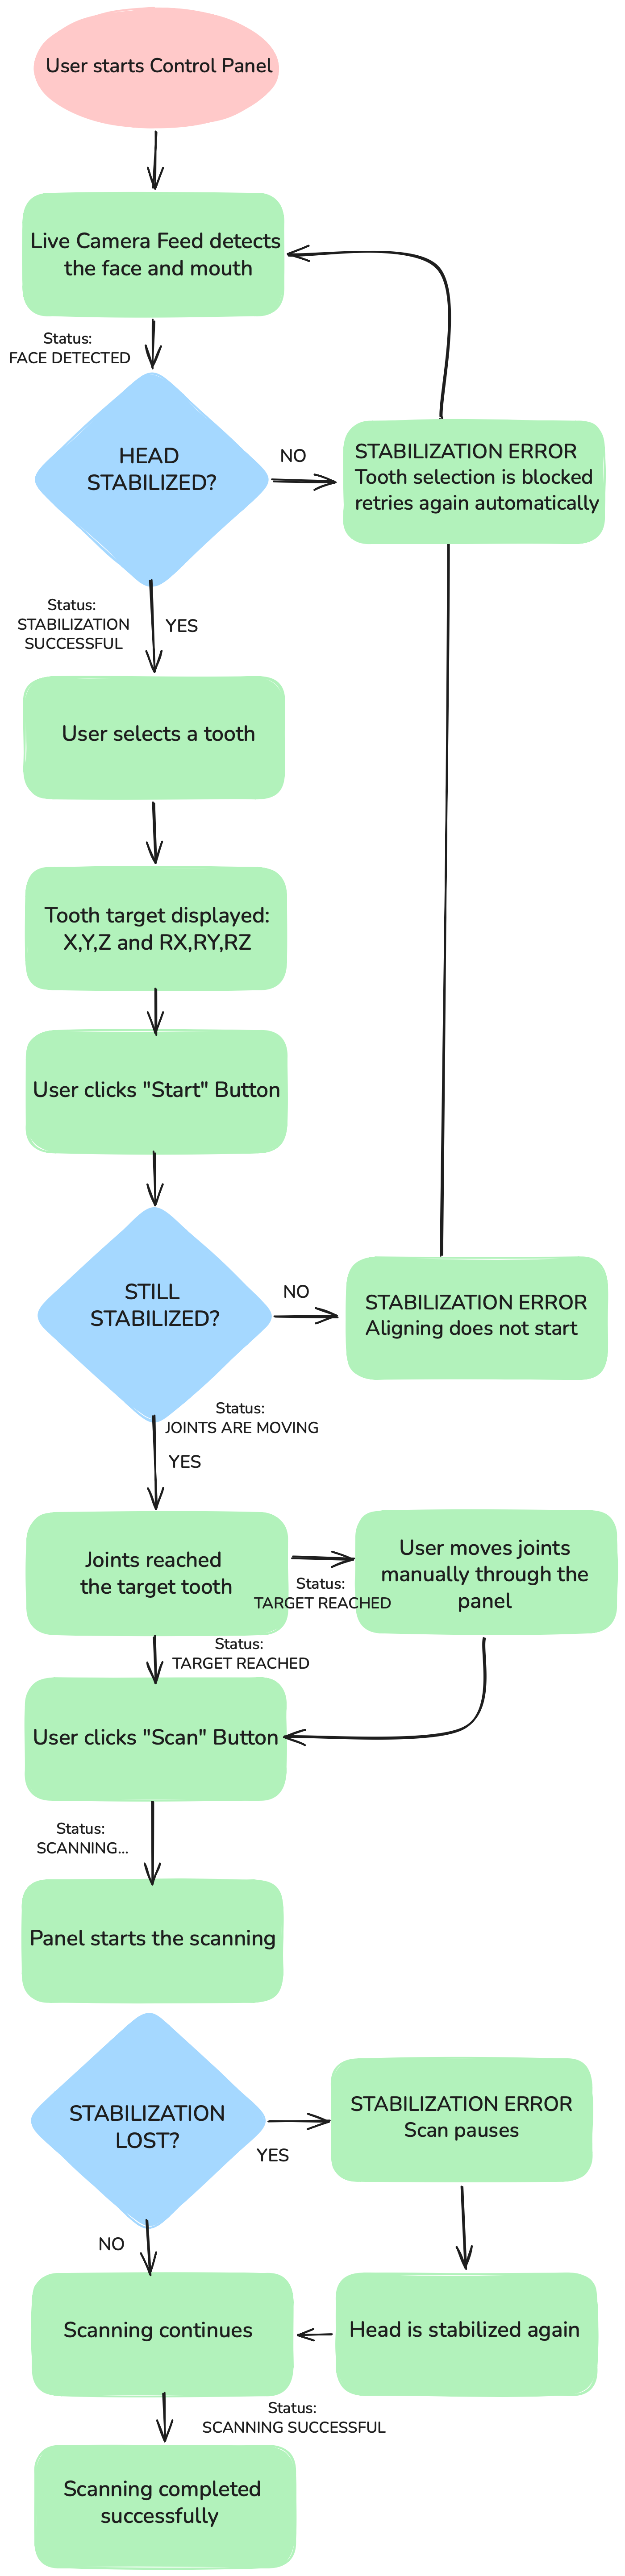
\includegraphics[width=\columnwidth,height=0.45\textheight,keepaspectratio]{ui_assets/user_flow.png}
    \caption{User Flow Diagramme (Excalidraw)}
    \label{fig:figma}
\end{figure}

Bu baglamda su designda su noktalara dikkat edilmistir: 

\begin{itemize}
    \item AA
\end{itemize}

Design Qt Creator ui dosyasi olusturup Layoutlar, Frameler, QLabellar etc. ile dizayn edilmistir. Figure~\ref{fig:qt}
Joystick widget gibi bazi ui componentleri complex olmalari nedeniyle py dosyasi ile olusturulmustur.


\begin{figure}[t]
    \centering
    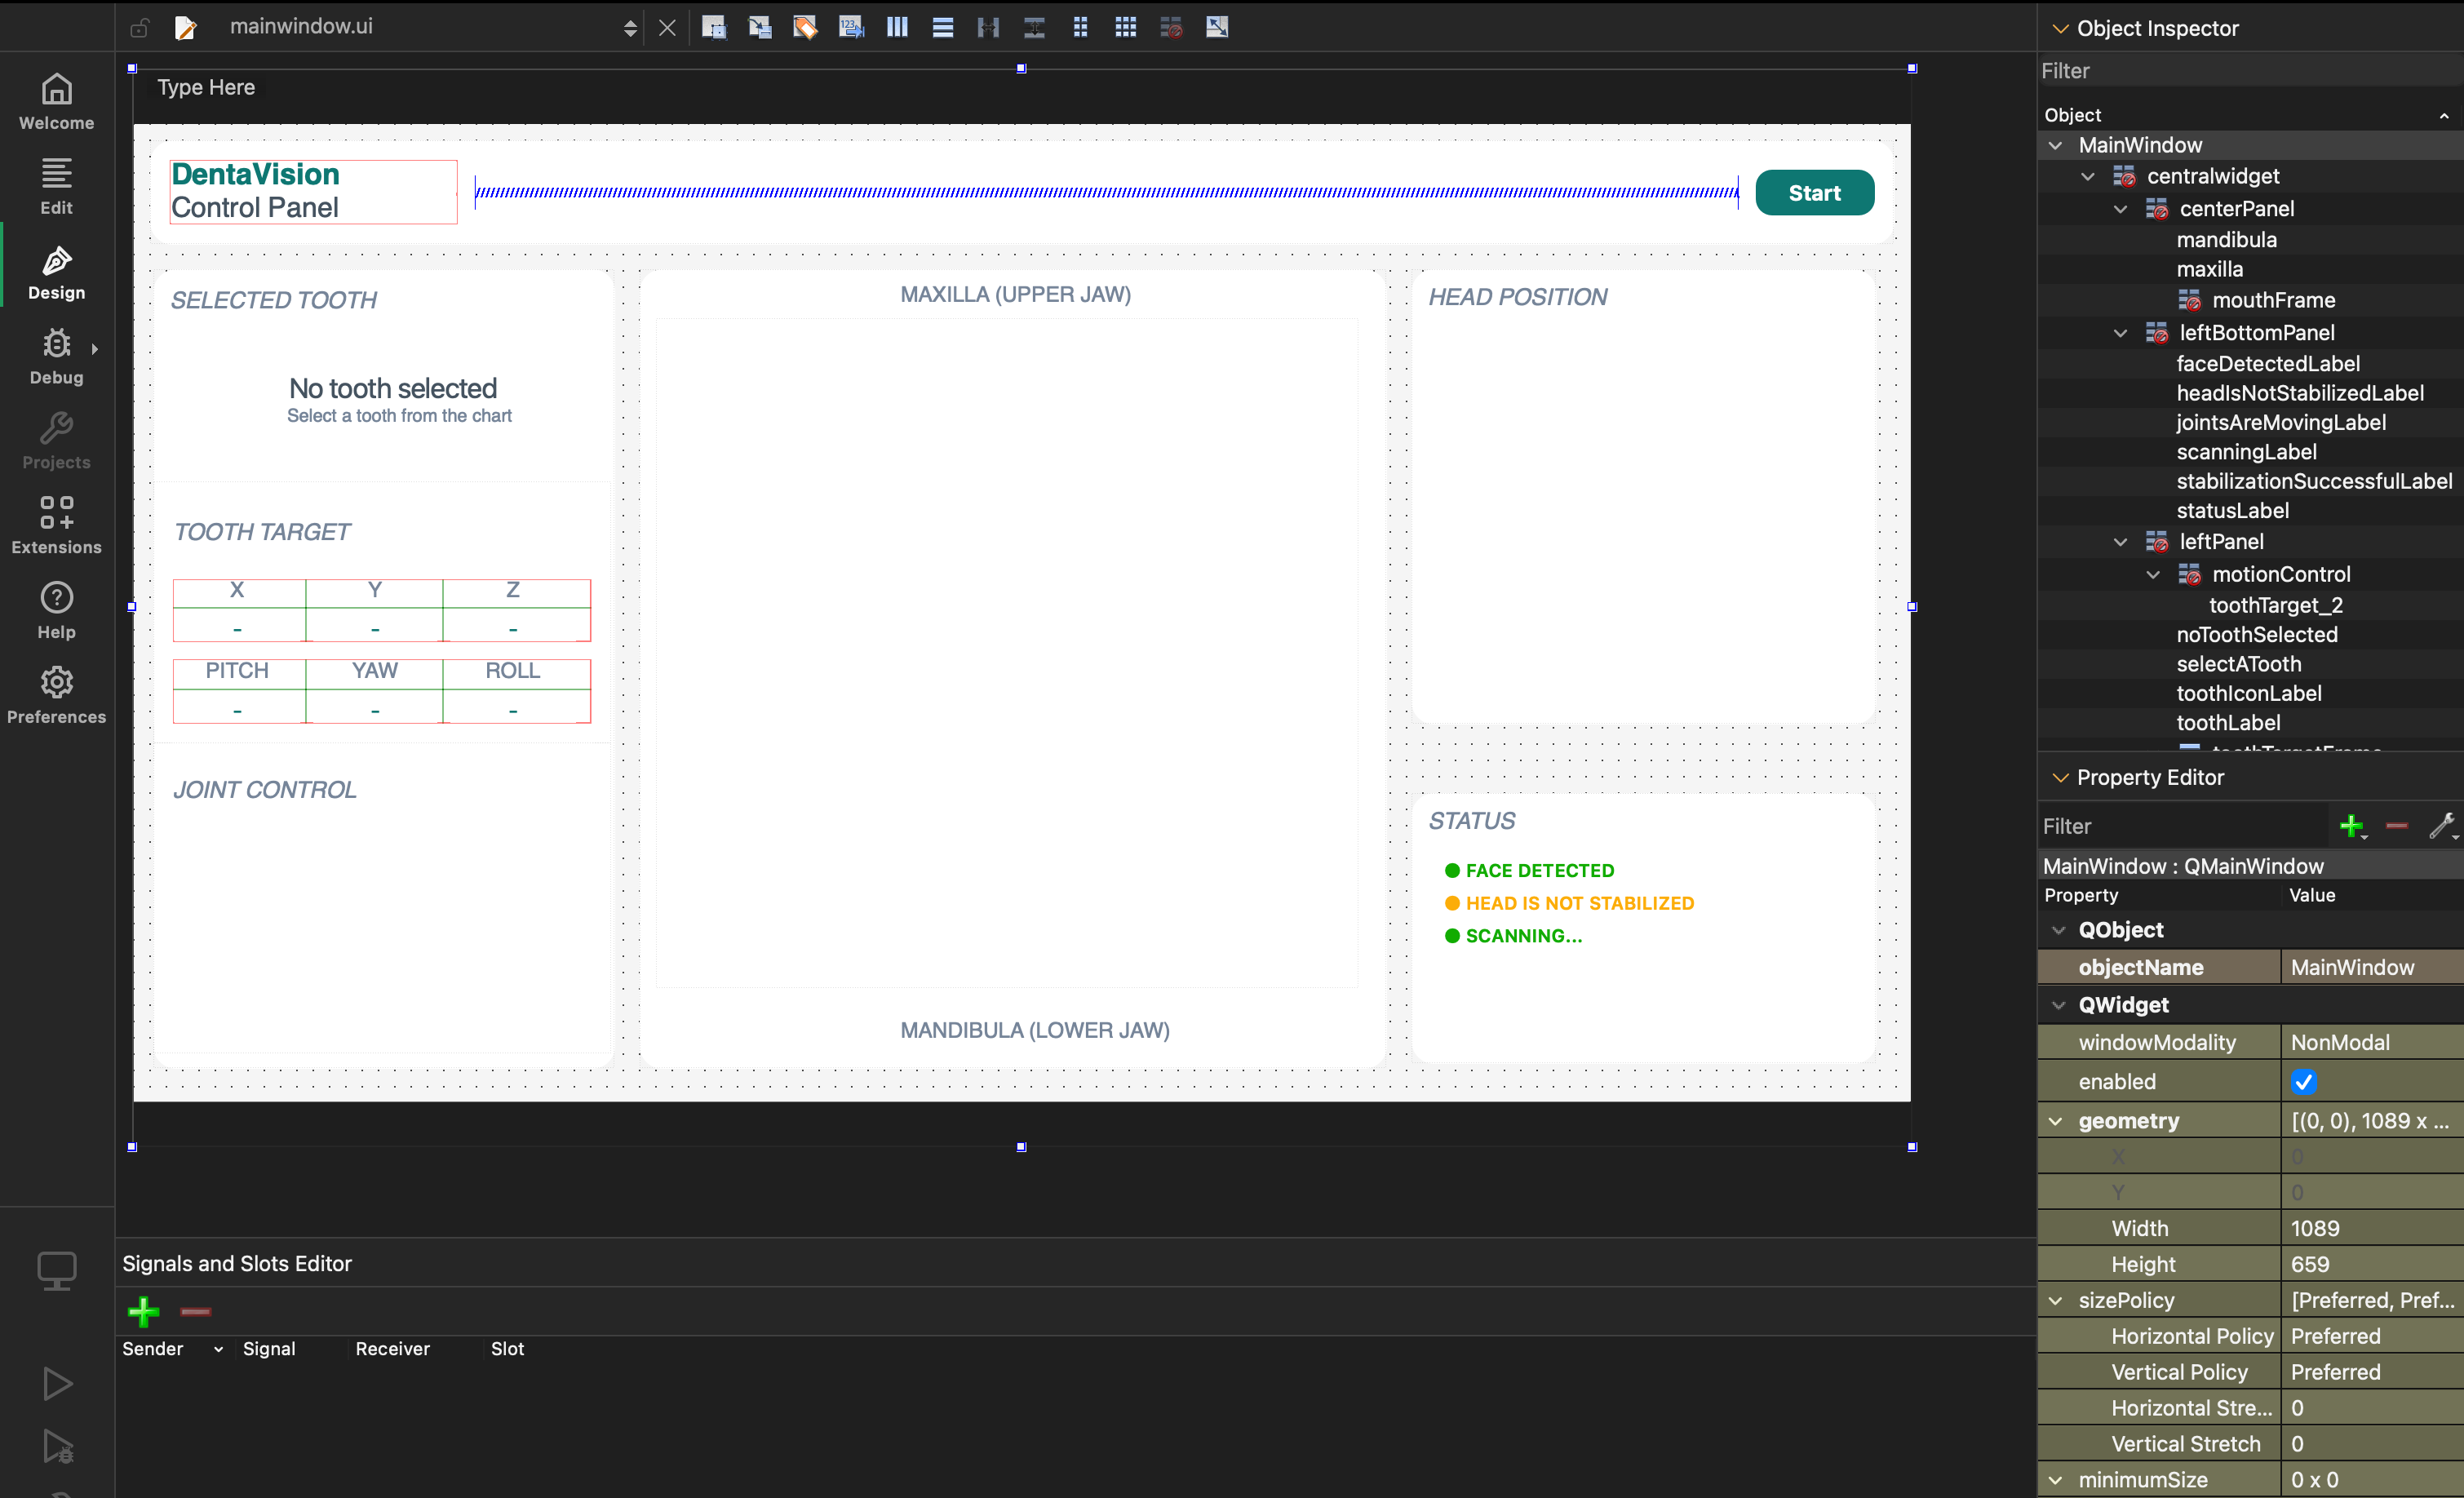
\includegraphics[width=\columnwidth,height=0.45\textheight,keepaspectratio]{ui_assets/qt.png}
    \caption{Qt Creator UI File}
    \label{fig:qt}
\end{figure}

\begin{figure}[t]
    \centering
    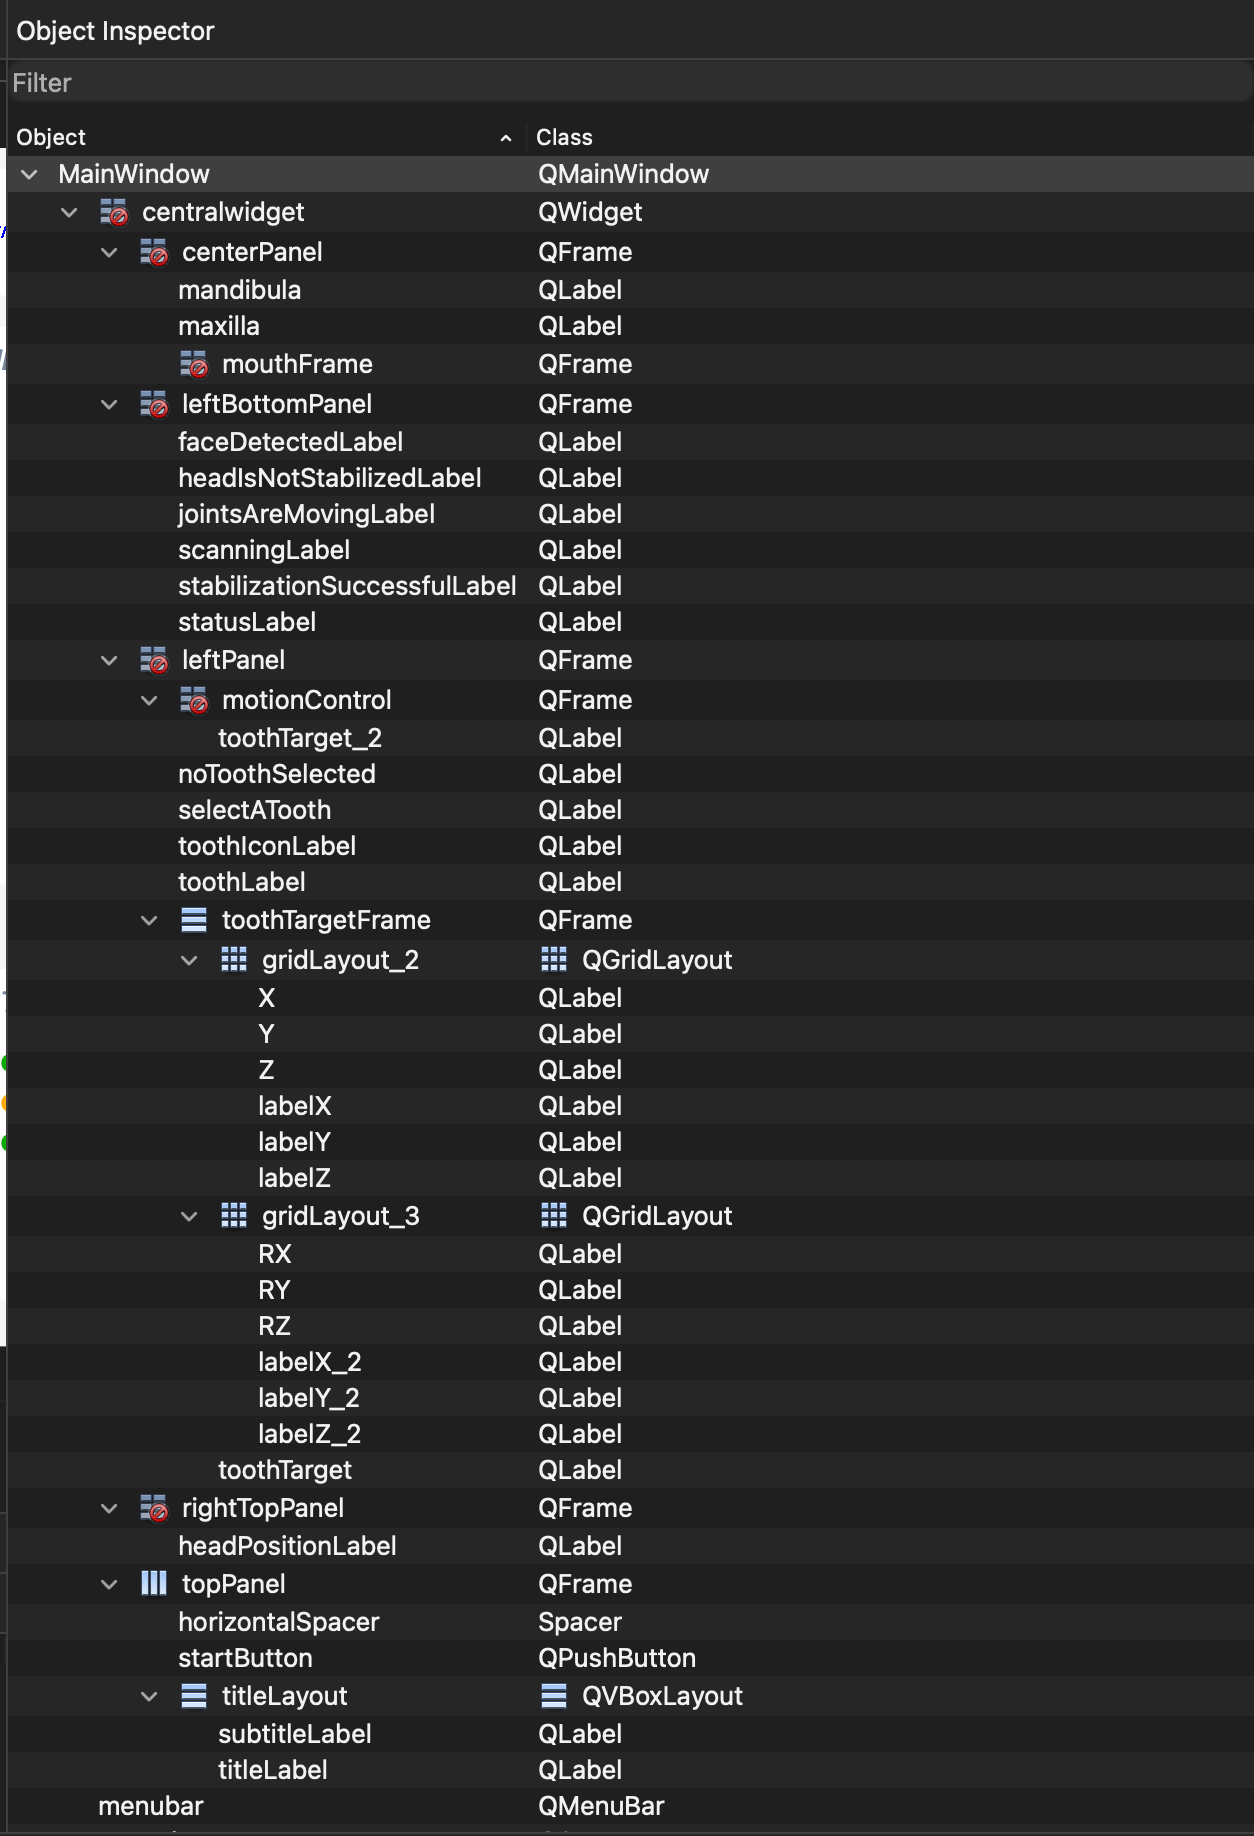
\includegraphics[width=\columnwidth,height=0.35\textheight,keepaspectratio]{ui_assets/object_inspector.png}
    \caption{Qt Creator Object Inspector}
    \label{fig:object_inspector}
\end{figure}

\subsection{Main Window Layout}
Main Window, islem akisini soldan saga ve ustten alta okunacak sekilde 3 panele böler: Solda sirasiyla ustten alta dis secim gostergesi, secilen dis icin tooth targeting sonuclarinin degerleri ve personelin manuel olarak joint hareketlerini kontrol edebilecegi bir motion control modulu bulunmaktadir.
Ortada ise hedeflenen disin secilmesine olanak saglayan tooth chart paneli bulunmaktadir ve son olarak sagda, canli kamera goruntusu ve sistem stateini gosteren status paneli olmak uzere iki panel bulunmaktadir.
En ustte layoutta ise Control Panelin logosu ve 3 asamali Start/Scan/Pause butonu bulunur. 

Main Window ilk once Figma'da ilk versiyonu Figure~\ref{fig:mainwindow_first} olusturulmustur. Bu layout supervisor feedbackleri ve gelisen proje degisiklikleriyle use case ve gercek hayat usabilitysine yonelik revize edilmistir. Figure~\ref{fig:mainwindow_current}

\begin{figure}[h]
    \centering
    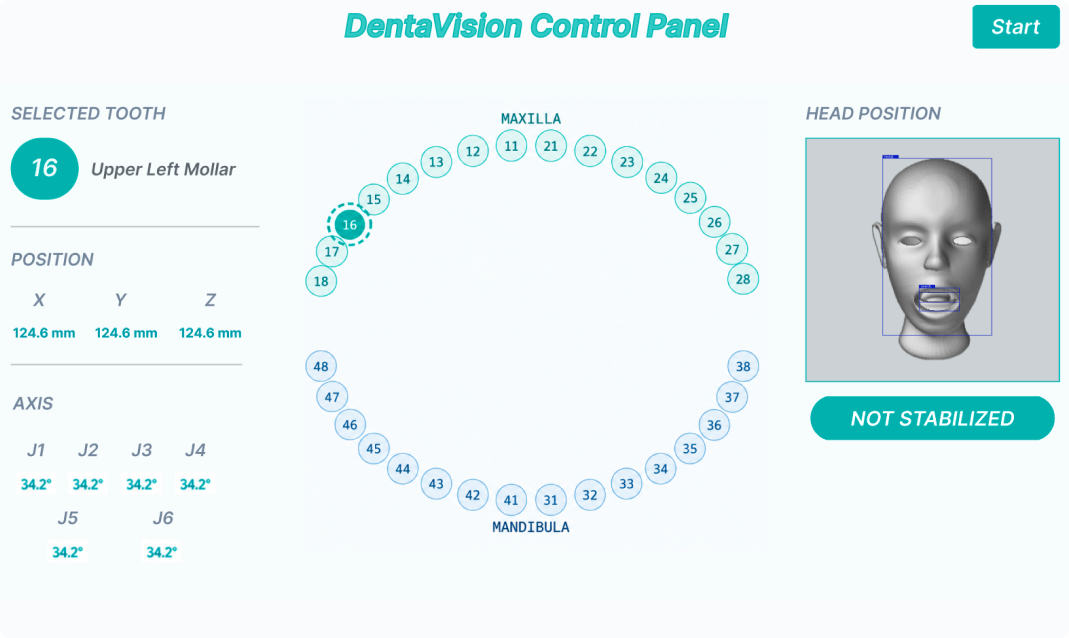
\includegraphics[width=\columnwidth,height=0.40\textheight,keepaspectratio]{ui_assets/first_version.png}
    \caption{First Version of MainWindow}
    \label{fig:mainwindow_first}
\end{figure}

Güncel:

\begin{figure}[h]
    \centering
    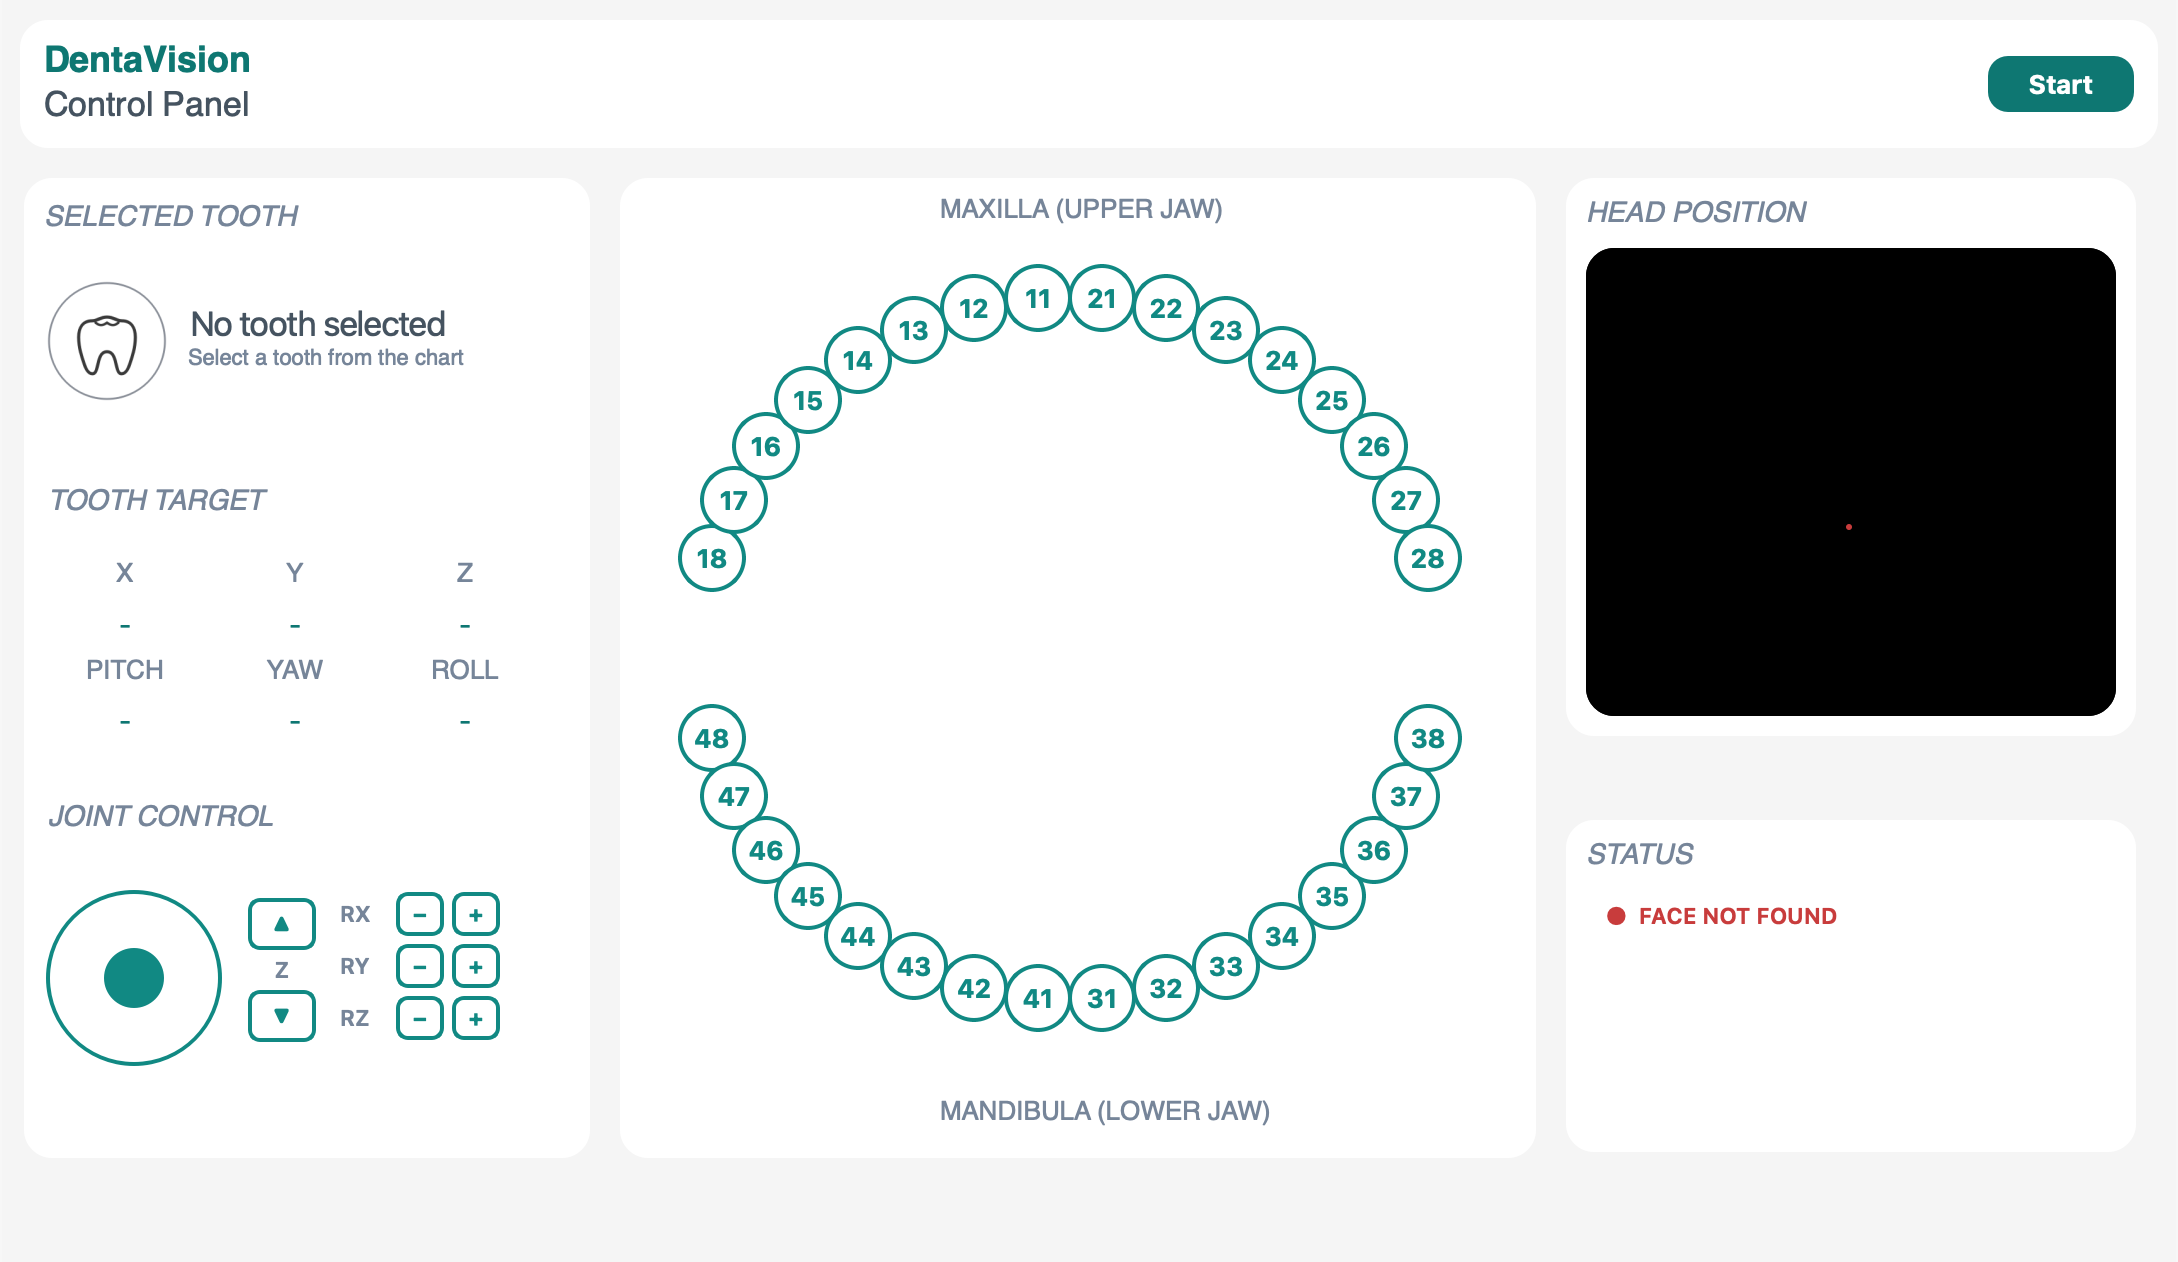
\includegraphics[width=\columnwidth,height=0.40\textheight,keepaspectratio]{ui_assets/current_ui_oP.png}
    \caption{Last Version of MainWindow}
    \label{fig:mainwindow_current}
\end{figure}

\subsection{Tooth Target Panel}

Bu panel 'selected tooth' altinda default (no tooth selected) dis figuru seklinde bir logo bulundurur Figure~\ref{fig:no_tooth_selected_badge}. 
Dental archtan bir dis secildiginde bu figur yerine secilen disin FDI numarasi gelir ve ismi yaninda yazdirilir. Figure~\ref{fig:tooth_selected_badge} 

\begin{figure}[h]
    \centering
    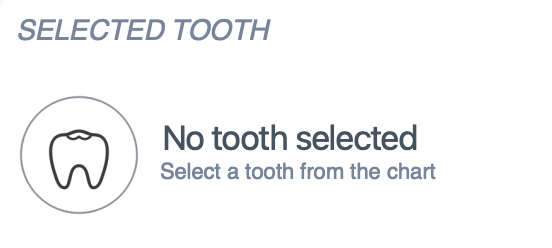
\includegraphics[width=\columnwidth,height=0.40\textheight,keepaspectratio]{ui_assets/components/no_tooth_selected.png}
    \caption{No Tooth Selected Badge}
    \label{fig:no_tooth_selected_badge}
\end{figure}

\begin{figure}[h]
    \centering
    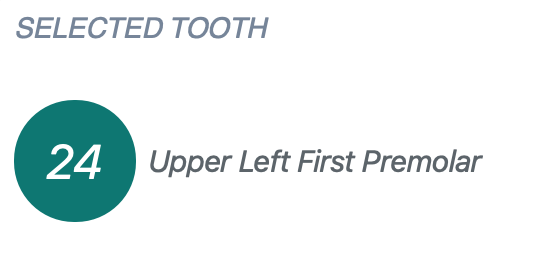
\includegraphics[width=\columnwidth,height=0.40\textheight,keepaspectratio]{ui_assets/components/tooth_selected.png}
    \caption{Tooth Selected View}
    \label{fig:tooth_selected_badge}
\end{figure}

Selected Tooth bolumunun altinda Tooth Target alani bulunur. Bu alan secilen dise gore hesaplanan hedef koordinatları, konum icin X,Y,Z ve rotation icin pitch, roll, yaw degerlerini panel kullanicisina gosterir.
Hicbir dis secilmemisken tum etiketlerin '-' olarak gosterilmesi tercih edilmistir. Figure\ref{fig:tooth_target_} bu, "henüz hesaplanmış geçerli bir değer yok" durumunu "0.0 mm" gibi hesaplanmış bir değerle karıştırmayı önleyen bilinçli bir tercihtir, çünkü 0.0 mm operatör tarafından gerçek bir ölçüm sonucu sanılabilir.
Ekrandan bir dis secildiginde etiketler, birimleriyle birlikte anlik olarak guncellenir. \ref{}    
 
\begin{figure}[h]
    \centering
    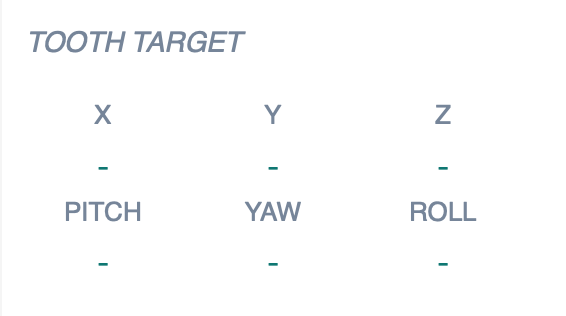
\includegraphics[width=\columnwidth,height=0.40\textheight,keepaspectratio]{ui_assets/components/tooth_target_.png}
    \caption{Tooth Target Landing/Default View}
    \label{fig:tooth_target_}
\end{figure}

\begin{figure}[h]
    \centering
    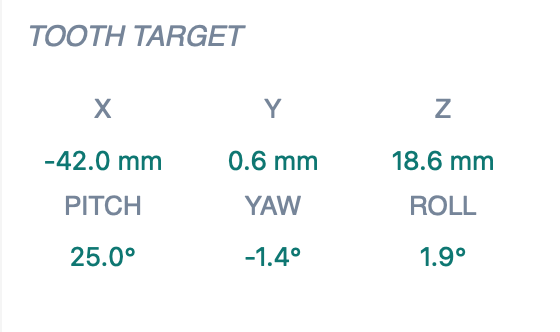
\includegraphics[width=\columnwidth,height=0.40\textheight,keepaspectratio]{ui_assets/components/tooth_target.png}
    \caption{Tooth Target View}
    \label{fig:tooth_target}
\end{figure}


\subsection{Manuel Joint Control Panel}

sistem su ..... asamalardayken kullanima aciktir. Manuel motion kontrol ayari yapilabilir.

\begin{figure}[h]
    \centering
    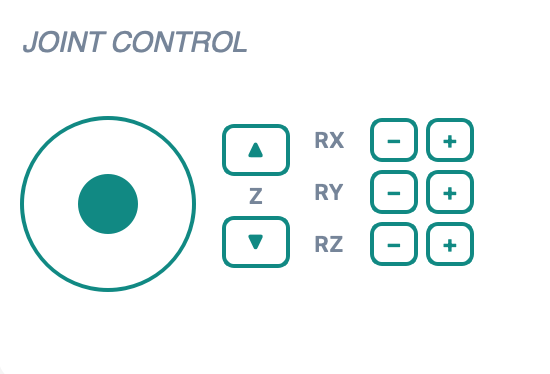
\includegraphics[width=\columnwidth,height=0.40\textheight,keepaspectratio]{ui_assets/components/joint_control.png}
    \caption{Joint Control Panel}
    \label{fig:joint_control}
\end{figure}

BURAYA TERMINAL CIKTISI DA EKLE 

Joint adjustments su caselerde yapilabilmektedir:

\begin{itemize}
    \item A
\end{itemize}

\subsection{Tooth Chart Panel}

Dis secim paneli, disleri duz bir liste veya tablo olarak degil, conceptul basitlestirilmis dental bir arkin (ust ve alt cene yayinin) geometrisine benzer eliptik bir duzen uzerinde konumlandirir. Figure~\ref{fig:dental_arch} 
Panelde dental arki anlamayi kolaylastiran maxilla (upper jaw) ve mandibula (lower jaw) labellari bulunmaktadir.
Bu tasarim personelin gorsel olarak disi daha hizli ve sezgisel bulmasina yardimci olmayi ongormektedir. Bu sayisal bir listeye gore cognitive load belirgin bir sekilde azaltir. 

\begin{figure}[h]
    \centering
    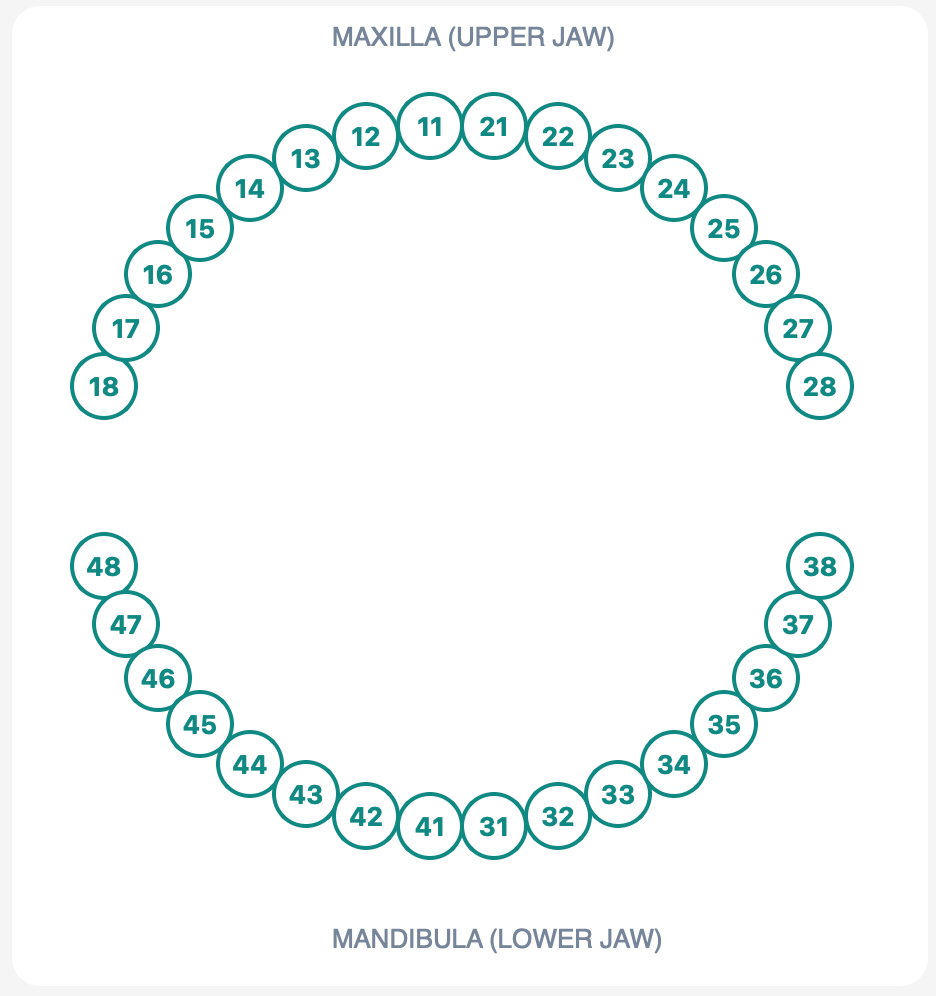
\includegraphics[width=\columnwidth,height=0.40\textheight,keepaspectratio]{ui_assets/components/dental_arch.png}
    \caption{Dental Arch Landing View}
    \label{fig:dental_arch}
\end{figure}

Bir dise tiklandiginda, (on\_tooth\_selected) hastanin kafa pozisyonu yeterince stabilse secilen disin ismi ve FDI numarasi bir badge Figure~\ref{fig:dental_arch_chosen} olarak gorunur.
Kafa pozisyonu yeterince stabil degilse sistem secimi bastan engeller, bu sayede hastanin kafasi hareket halindeyken guvenilir olmayan bir Tooth Target uzerinde calisilmasinin onune gecilmesi ongorulur.
Bu casein error mesaji terminale yazdirilirken, gercek hayattaki karsiliginda panelde secime izin verilmez ve Status olarak "head not stabilized" notificationu sayesinde personel bunun bilincine varir.  


\begin{figure}[h]
    \centering
    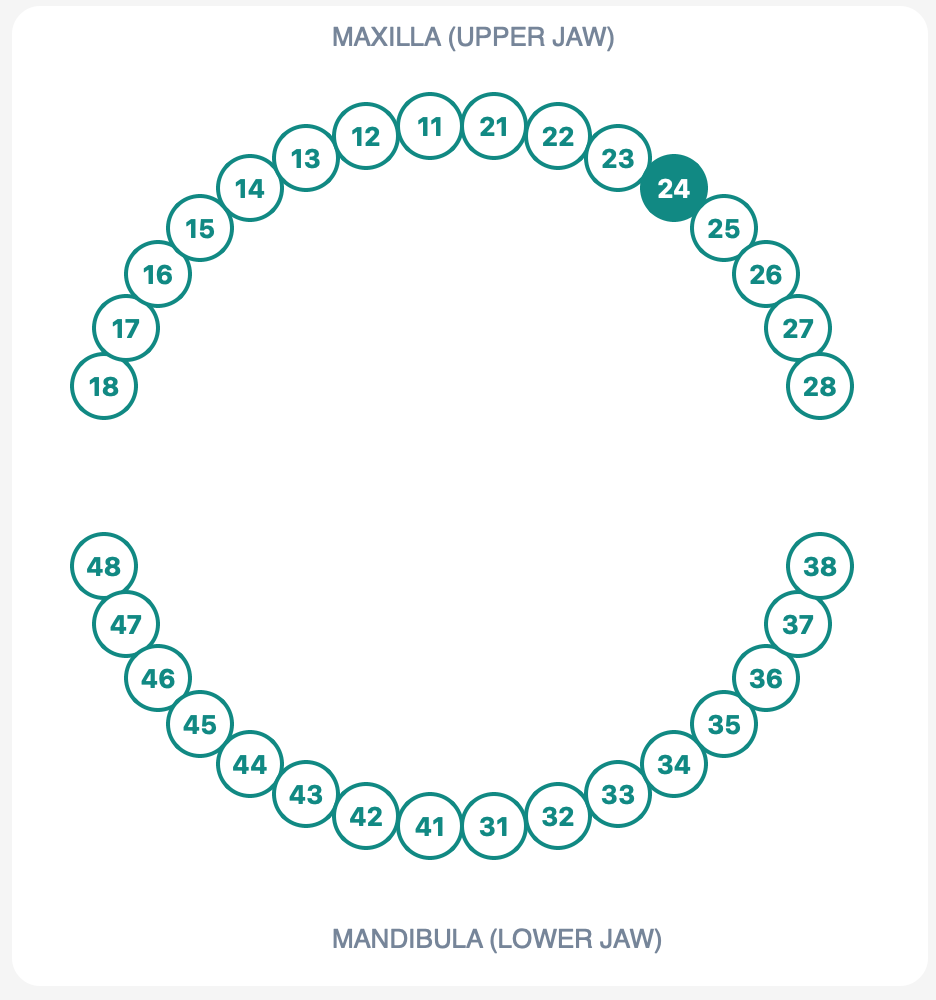
\includegraphics[width=\columnwidth,height=0.40\textheight,keepaspectratio]{ui_assets/components/dental_arch_chosen.png}
    \caption{Dental Arch Tooth Chosen View}
    \label{fig:dental_arch_chosen}
\end{figure}

\subsection{Camera Panel and Status Indicators}

The Camera Panel consists of a live video feed with bounding boxes highlighting the detected face and mouth, with rounded corners framing the detected regions. Figure~\ref{fig:camera} illustrates the interface. In addition, a red point is displayed on the screen to indicate the target position at which the patient's mouth should be centered. This visual reference is intended to assist in monitoring the stability of the patient's head position. A default positional tolerance of 15 pixels is defined around the target point;
 therefore, the patient's mouth is considered to remain within the acceptable stabilization range when its detected position stays within this tolerance.
Tespit durumuna gore FACE NOT FOUND \ref{}, FACE DETECTED \ref{}, STABILIZATION SUCCESSFUL \ref{}, STABILIZATION ERROR \ref{} etiketleri, renk kodlamasiyla desteklenir ve status bolumunde gosterilir.

\begin{figure}[h]
    \centering
    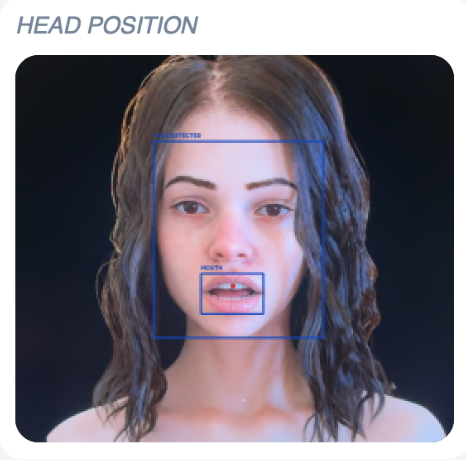
\includegraphics[width=\columnwidth,height=0.40\textheight,keepaspectratio]{ui_assets/components/camera.png}
    \caption{Camera View with a Human Face Model generated by AI. (Status: Head is not stabilized)}
    \label{fig:camera}
\end{figure}


Start butonuna tiklanilarak jointlere hareket komutu verildikten sonra sirasiyla JOINTS ARE MOVING \ref{} ve TARGET REACHED \ref{} etiketleri statuste belirir.
Sonrasinda kullanici gerekli tatbikleri yaptiktan sonra Scan butonuna basar ve sorunsuz ilerlerse statuste sirasiyla SCANNING... \ref{} ve SCANNING SUCCESSFUL \ref{} belirir. 


Status bolumu Camera panelinin hemen altinda bulunur ve personelin sistemdeki akisi ve hastanin guvenligini kontrol etmesine katkida bulunan bir gostergec olarak dusunulmustur.
Status barinin akis hikayesi su sekildedir:

\begin{enumerate}
    \item default olarak kirmizi renkte FACE NOT FOUND etiketi ile baslar. 
    \item Kamerada bir yuz detect edildiginde yesil FACE DETECTED etiketi status barina eklenir.
    \item Eger hastanin kafasi 
\end{enumerate}




\subsection{Buttons}

\begin{figure}[h]
    \centering
    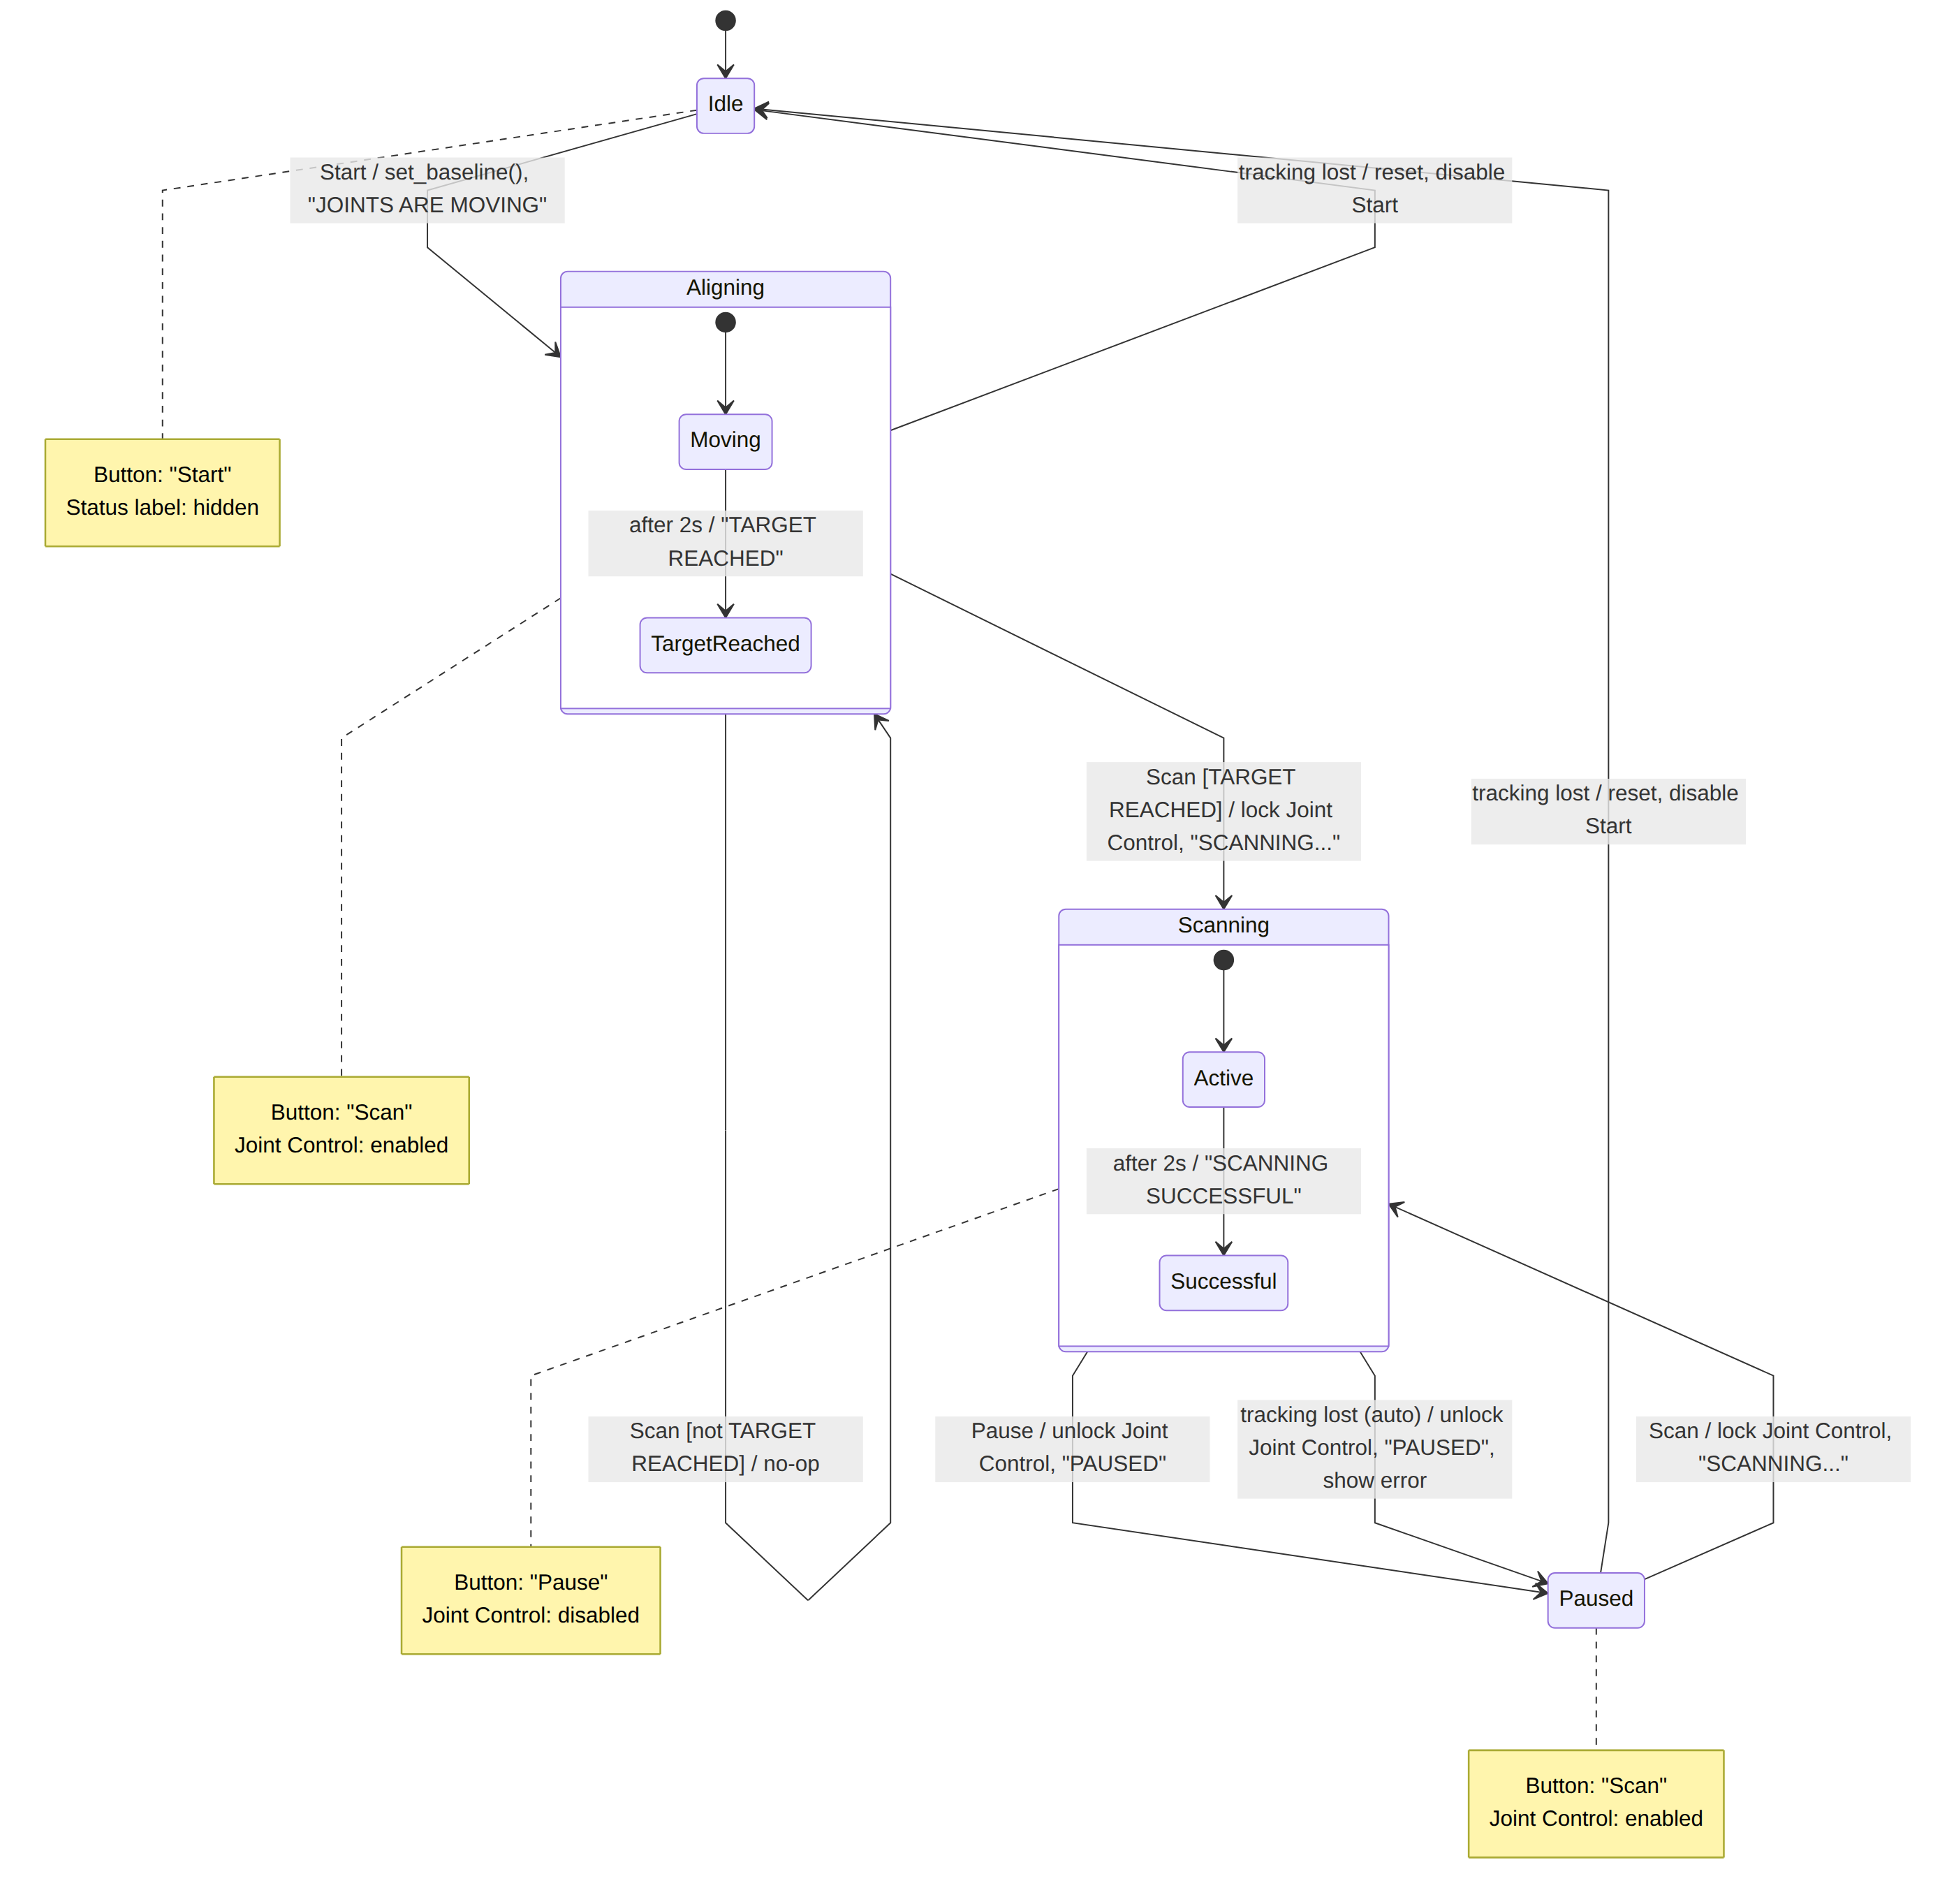
\includegraphics[width=\columnwidth,height=0.45\textheight,keepaspectratio]{ui_assets/state_buttons.png}
    \caption{State Diagram of Button Transformation created by Claude AI}
    \label{fig:buttons}
\end{figure}

\begin{figure}[h]
    \centering
    
\includegraphics[width=0.45\columnwidth,height=0.45\textheight,keepaspectratio]{ui_assets/components/button_start.png}
    \caption{Start Button View}
    \label{fig:button_start}
\end{figure}

\begin{figure}[h]
    \centering
    
\includegraphics[width=0.45\columnwidth,height=0.45\textheight,keepaspectratio]{ui_assets/components/button_start_faded.png}
    \caption{Start Button Faded View}
    \label{fig:button_start_faded}
\end{figure}

\begin{figure}[h]
    \centering
    
\includegraphics[width=0.45\columnwidth,height=0.45\textheight,keepaspectratio]{ui_assets/components/button_scan.png}
    \caption{Scan Button View}
    \label{fig:button_scan}
\end{figure}

\begin{figure}[h]
    \centering
    
\includegraphics[width=0.45\columnwidth,height=0.45\textheight,keepaspectratio]{ui_assets/components/button_pause.png}
    \caption{Pause Button View}
    \label{fig:button_pause}
\end{figure}


\section{Vision and Head Tracking}
Yüz tespiti, \texttt{FaceTracker} sınıfının oluşturduğu MediaPipe Face Mesh
nesnesiyle (\texttt{static\_image\_mode=False}, \texttt{max\_num\_faces=1})
yapılır. 

\subsection{Face and Mouth Detection}

\subsection{Calibration}

\subsection{Position Estimation}

\subsection{Orientation Estimation}

\subsection{Stabilization Check}



\section{Calculation of Tooth Target}
Tooth Target, seçilen bir diş için robot kolunun ulaşması gereken hedef
konumu olan X, Y, Z ve o anki kafa oryantasyonu olan RX, RY, RZ degerlerini
ifade eder. Hesaplama iki dosyaya bölünmüştür: 

Core'da bulunan \texttt{compute\_tooth\_target()} fonksiyonu asıl hesabı yaparken,
\texttt{tooth\_target\_controller.py} ise bu sonucu ne zaman
hesaplatacağını ve panele nasıl yazacağını yönetir.

\texttt{compute\_tooth\_target(tooth\_number, head\_position)} fonksiyonu
oldukça basit bir toplama işlemi yapar: \\

  x = \text{head\_position}.x + dx,

  y = \text{head\_position}.y + dy,
  
  z = \text{head\_position}.z + dz
\\

Buradaki dx ve dy değerleri \texttt{TOOTH\_OFFSETS\_MM} sözlüğünden,
$dz$ değeri ise \texttt{TOOTH\_DEPTH\_OFFSETS\_MM} sözlüğünden, diş
numarasına göre okunur. Bu iki sözlük coreda teeth data olarak kayitlidir. 
Bu data sabit bir dental arch modelinden üretilmiştir ve her
dişin ağız merkezine göre sabit bir konumu olduğunu varsayar.

Kafa takibinden gelen veri (\texttt{head\_position}) ile diş anatomisinden gelen sabit veri
(dx, dy, dz) burada bir araya gelir. \texttt{head\_position} nesnesi
dişler hakkında hiçbir şey bilmez, \texttt{teeth\_data.py} da kafa
pozisyonu hakkında hiçbir şey bilmez. Tooth Target, bir kere hesaplanıp ekranda sabit kalan bir değer
değildir; iki farklı durumda yeniden hesaplanır:
 
\begin{itemize}
    \item \textbf{Diş seçildiğinde:} Kullanıcı bir dişe tıkladığında
    \texttt{show\_target\_for(tooth)} metodunu tetiklenir.
    Bu metot \texttt{compute\_tooth\_target()} sonucunu alır ve
    X,Y ve Z labellarina mm degeri olarak yazar.
    \item \textbf{Kafa pozisyonu her güncellendiğinde:} Kamera
    döngüsü her karede yeni bir kafa pozisyonu hesapladığında, \texttt{CameraController}
    bir callback tetikler. Eğer o anda bir diş seçiliyse ve kafa hâlâ stabilize durumdaysa,
    \texttt{show\_target\_for()} tekrar çağrılır ve panel yeni
    değerlerle güncellenir.
\end{itemize}

Bu ikinci nokta önemlidir: Tooth Target, tıklama anında alınan tek bir
"fotoğraf" değildir; diş seçiliyken ve kafa stabilize kaldığı sürece her
karede yeniden hesaplanan, canlı bir değerdir. Kafa hafifçe hareket
ederse (ama stabilizasyon toleransı içinde kalıyorsa), panelde gösterilen
mm değerleri de buna göre anlık güncellenir.

Pozisyon ve oryantasyon iki deger grubu aynı
panelde birlikte gösterilir, ama kaynakları ve hesaplanma mantıkları
birbirinden bağımsızdır. Cünkü oryantasyon dişe değil sadece kafanın o
anki duruşuna bağlıdır.

RX RY ve RZ rotation degerleri vision bolumunde \texttt{estimate\_head\_orientation()} ile üç açıyı üç farklı yöntemle üretiliyor, ikisi gerçek ölçüm değil yaklaşıklık belirtiyor:

RZ yani roll degeri İki ağız köşesinin (landmark 61 ve 291) piksel koordinatları arasındaki açı doğrudan hesaplanıyor.
Yani ağız çizgisi yataydan ne kadar sapmışsa bir diger deyisle kafa sağa veya sola yatmışsa, o açı direkt \textit{atan2} ile derece cinsine çevriliyor.

RY yani yaw ne RX yani pitch 2d landmark verisiyle gercek aci olcumu mumkun olmadigindan sonuc ağız merkezinin (mouth\_mid), tespit edilen yüz kutusunun merkezine göre ne kadar kaydığına bakılarak yaklasik bir deger hesaplamaktadir.

Bu olcum gercek hayatta \textit{cv2.solvePnP} ile yapilmaktadir (daha da detaylandir)

Kafa artık güvenilir şekilde takip edilemezken panelde eski ve artık geçersiz olan bir mm veya derece
değerinin görünür kalmamaktadir; Bunun yerine kullanici ekranda "-" görür ve bunun henüz
hesaplanmamış ya da artık geçerli olmayan bir değer olduğunu anlar,
gerçek bir ölçümle karıştırmaz.

\section{Manuel Joint Control Mechanism}
Joint Control paneli, personelin seçilen dişe göre hesaplanan Tooth
Target'ı elle ince ayar yapabilmesini sağlar. Bu mekanizma iki dosyaya bölünmüştür:

\texttt{MotionController} sinifi tüm butonları ve joystick'i oluşturup
hareketleri hesaplar, \textit{ui/} folderinda bulunan joystick widget file i ise sınıfı ise X/Y ekseni için kullanılan dairesel
joystick'in çizimini ve mouse etkileşimini yönetir.
  
Panelde iki farklı kontrol biçimi bir arada kullanılır, ve bunlar
bilinçli olarak farklı tasarlanmıştır. X ve Y eksenleri için bir
\textbf{joystick} kullanılır: bu, sürekli ve orantılı (proportional) bir
kontroldür — joystick ne kadar ittirilirse, o yöndeki ofset de o oranda
büyür, ve joystick bırakıldığı anda ofset tekrar sıfıra döner. Z ekseni
ile RX/RY/RZ dönüşleri için ise \textbf{artımlı (incremental) buton}
kontrolü kullanılır: her tıklama sabit bir adım kadar (\texttt{Z\_STEP\_MM
= 1.0} mm, \texttt{ROTATION\_STEP\_DEG = 5.0}°) değeri artırır ya da
azaltır, ve bu değer bir sonraki tıklamaya kadar olduğu gibi kalır. Bu
ayrım rastgele değildir: X/Y ince ayarı doğası gereği sürekli ve
orantılı bir harekettir (joystick bunun için daha doğal bir arayüzdür),
oysa derinlik ve dönüş ayarları genelde küçük, adım adım düzeltmelerdir
ve bir buton bu amaca daha uygun düşer.

\texttt{MotionController}, her eksen için iki ayrı değer tutar: bir
\textbf{baseline} (taban değer) ve bir \textbf{jog} (o ana kadar
yapılan manuel düzeltme). Operatör "Start"a bastığında
\texttt{set\_baseline(x, y, z, rx, ry, rz)} çağrılır; bu, o anki Tooth
Target değerlerini baseline olarak kaydeder ve aynı zamanda tüm jog
değerlerini sıfırlar (\texttt{\_z = 0.0}, üç rotasyon ekseni de
\texttt{0.0}). Yani her yeni "Start" ile manuel düzeltmeler baştan
başlar; bir önceki taramadan kalan jog miktarı bir sonrakine taşınmaz.
Ekranda/terminalde gösterilen değer her zaman şu formülle hesaplanır:
\[
  \text{Gösterilen değer} = \text{Baseline} + \text{Jog}
\]

\section{Error Handling and Edge Cases}

\section{Limitations and Assumptions}
oryantasyon dişe göre değil sadece kafaya göre hesaplanıyor, farklı dişler için farklı yaklaşma açısı yok
joystick modeli hasta icin bir guven problemi olusturur mu?
\section{Testing and Validation}


\begin{figure}[t]
    \centering
    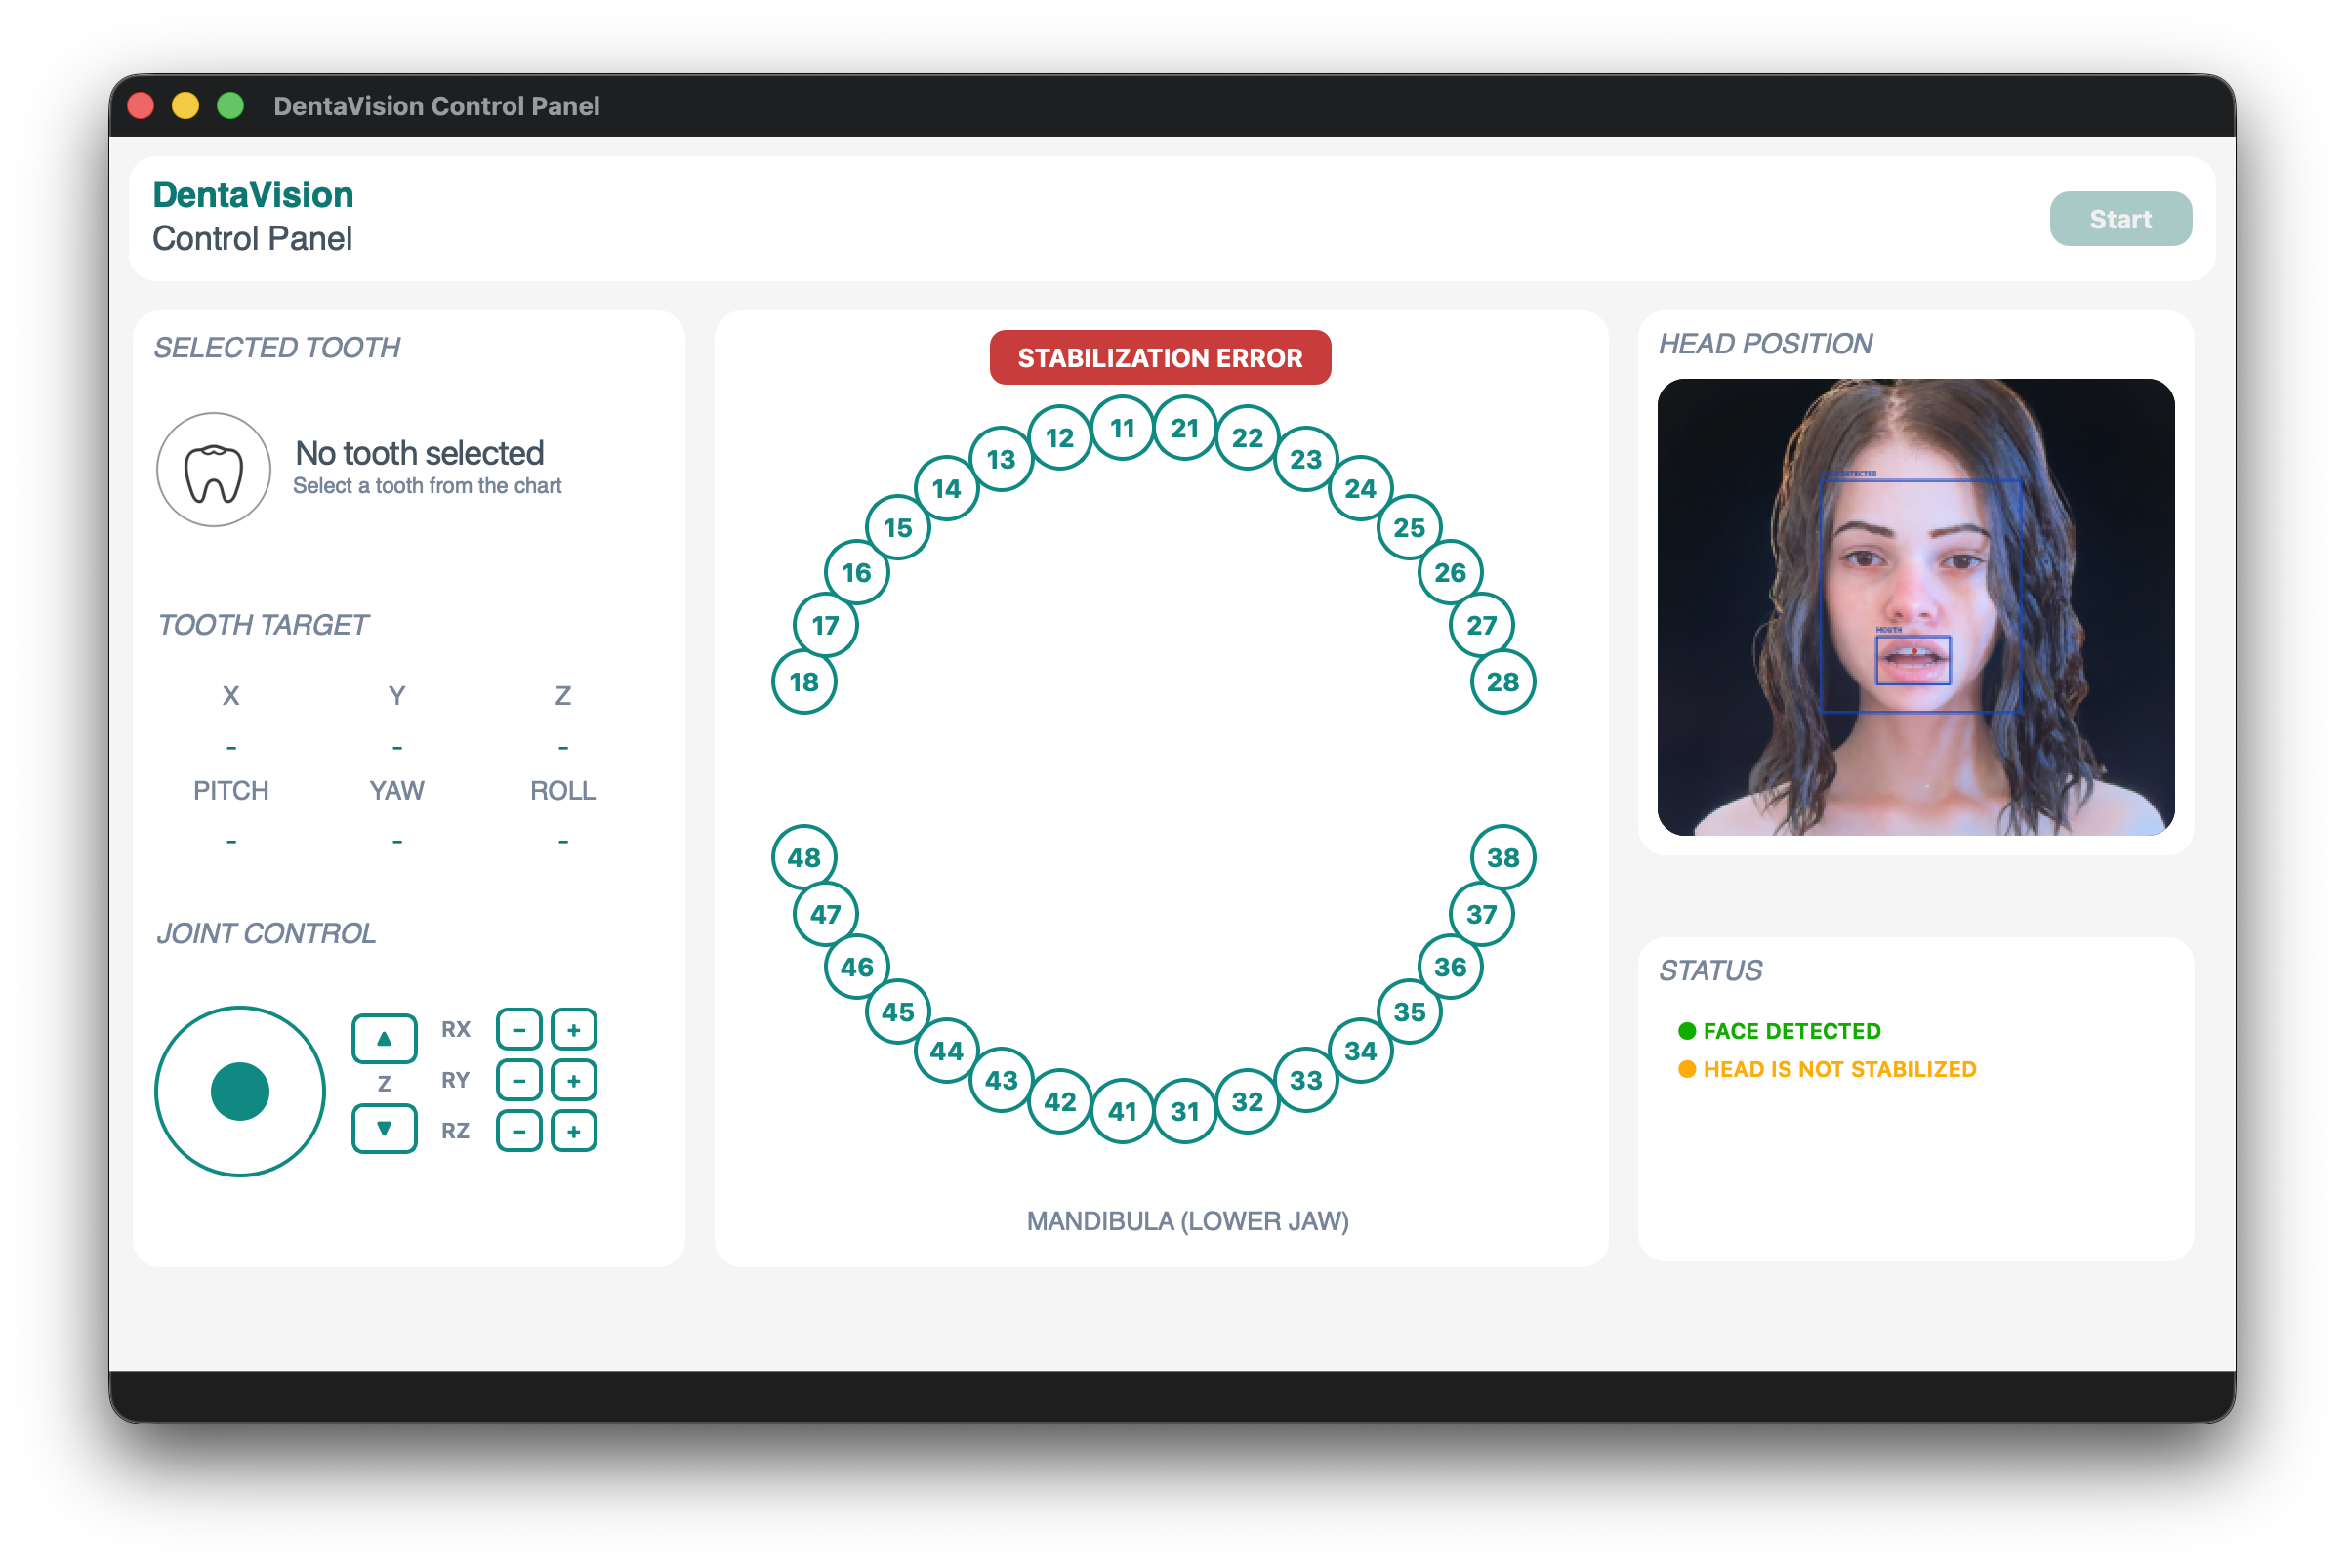
\includegraphics[width=\columnwidth,height=0.45\textheight,keepaspectratio]{ui_assets/demo2-5.png}
    \caption{Demo}
    \label{fig:demo_first}
\end{figure}

\begin{figure}[t]
    \centering
    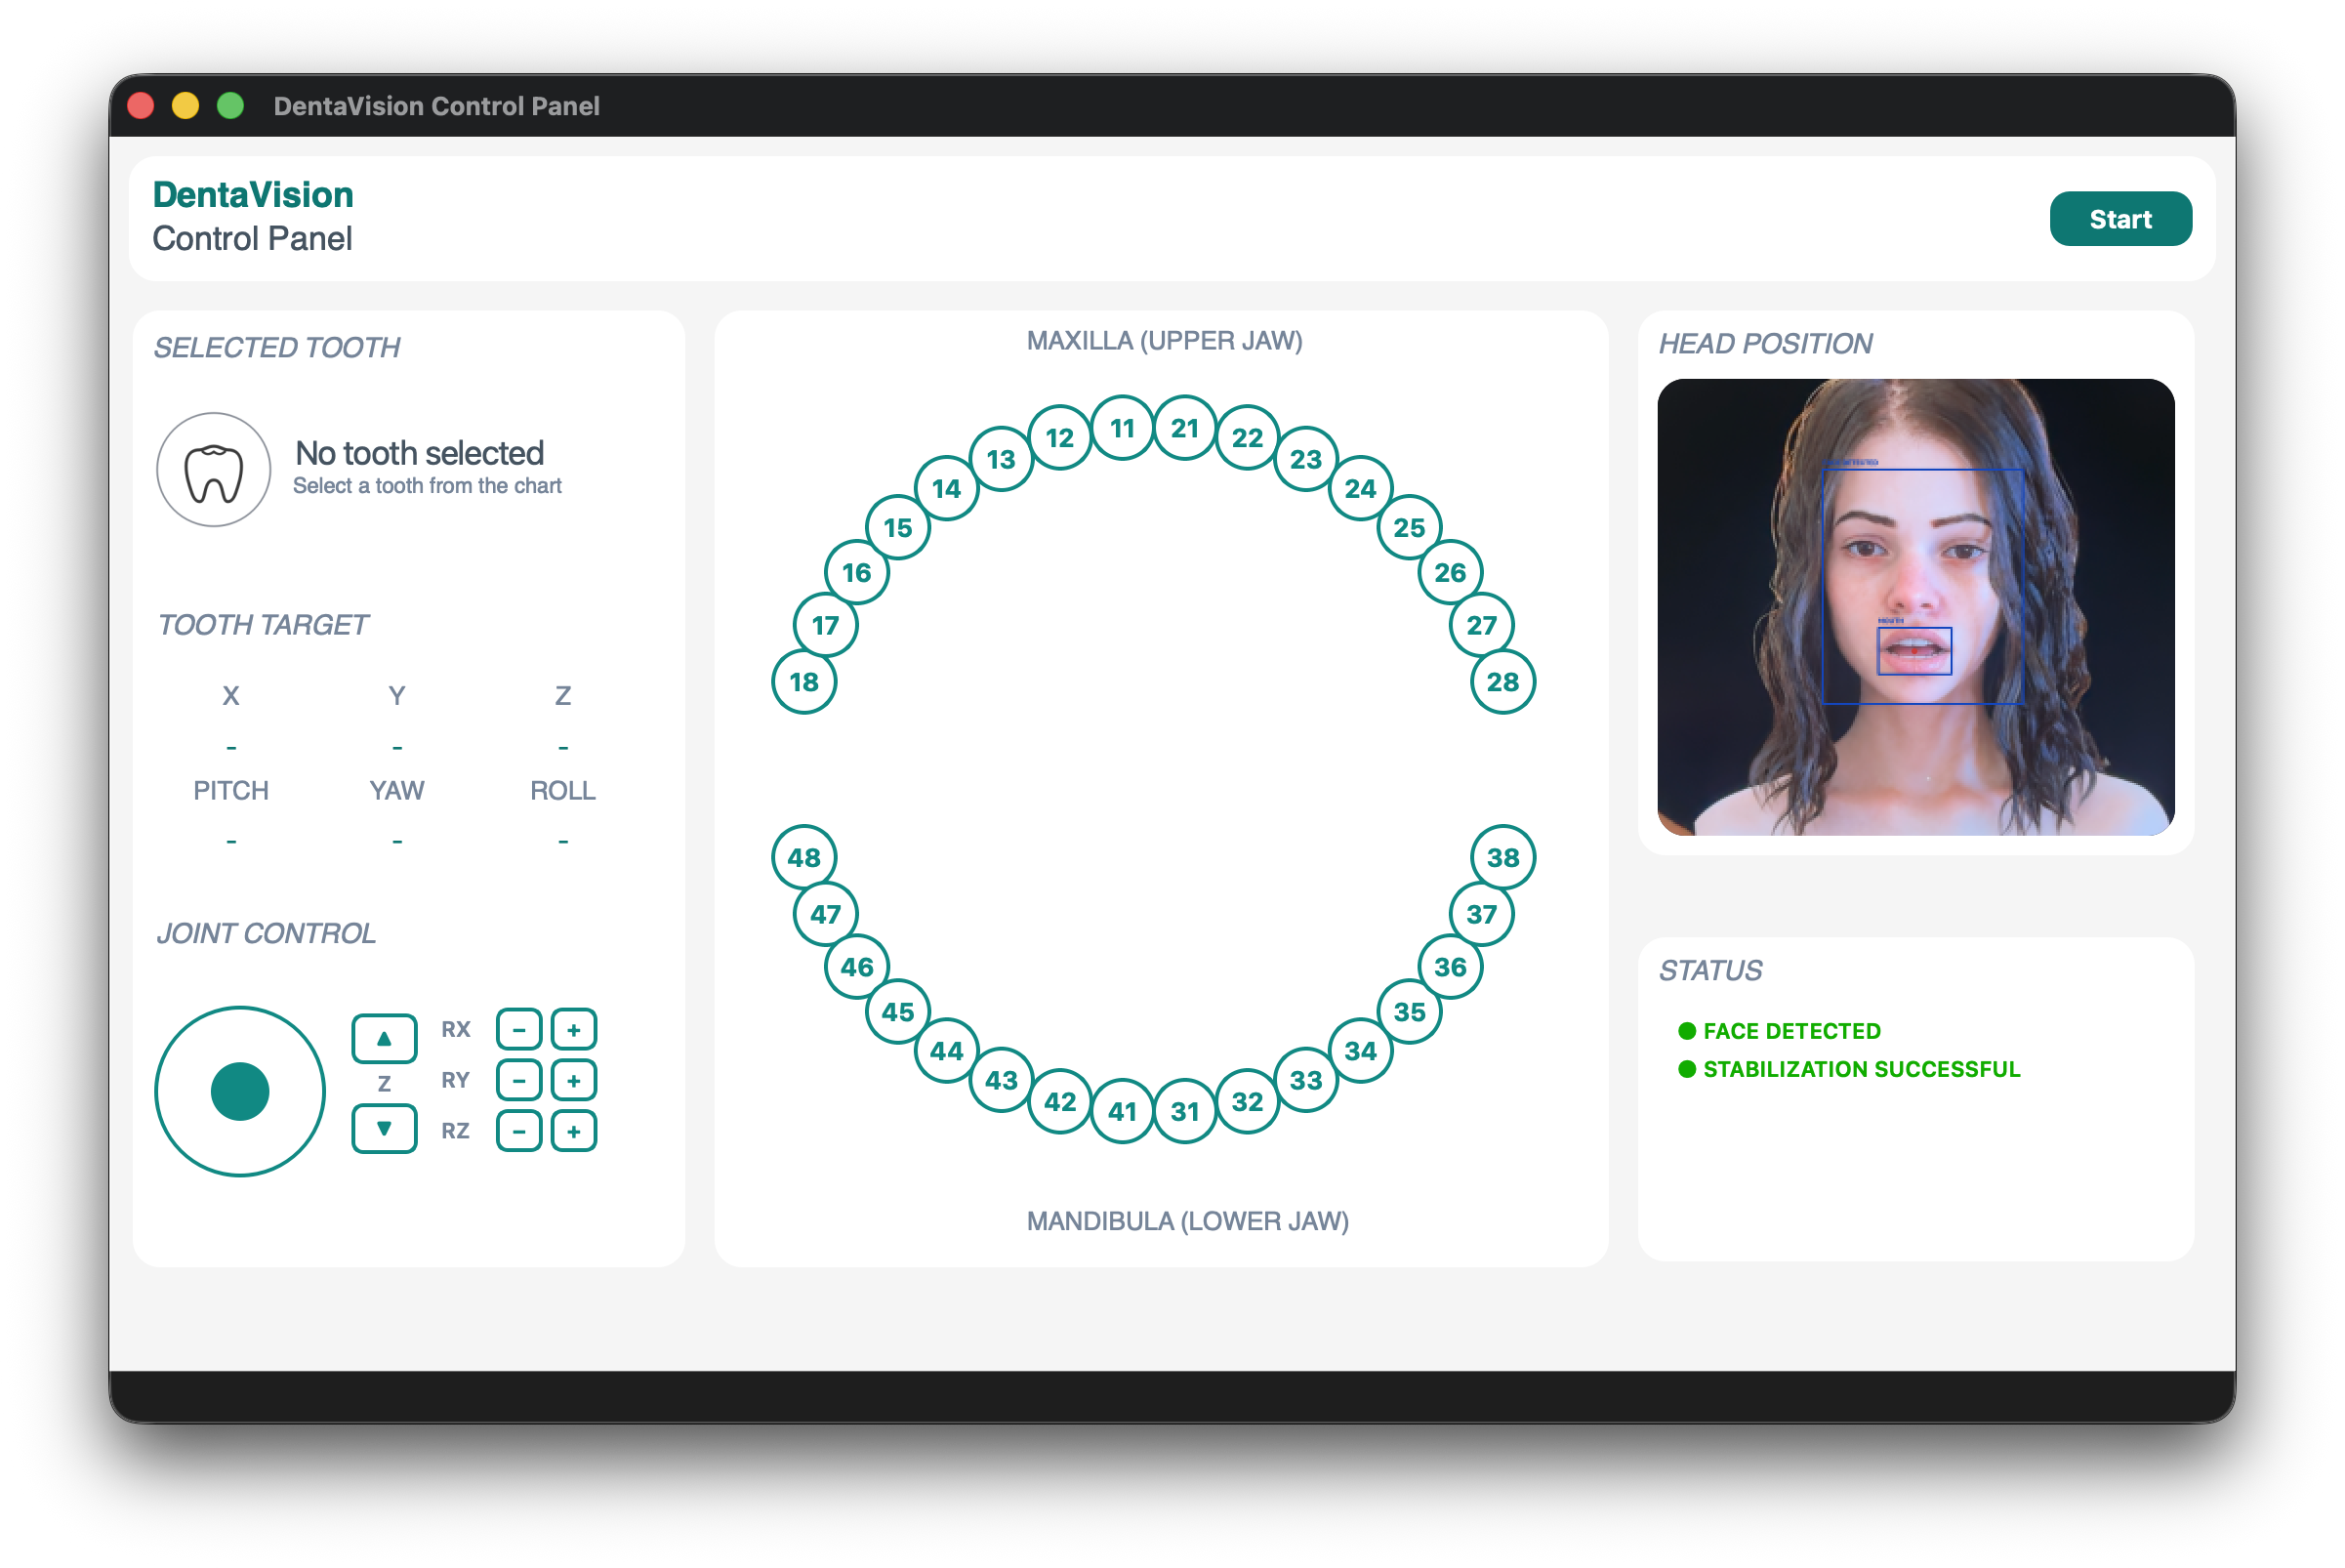
\includegraphics[width=\columnwidth,height=0.45\textheight,keepaspectratio]{ui_assets/demo3.png}
    \caption{Demo}
    \label{fig:demo_second}
\end{figure}

\begin{figure}[t]
    \centering
    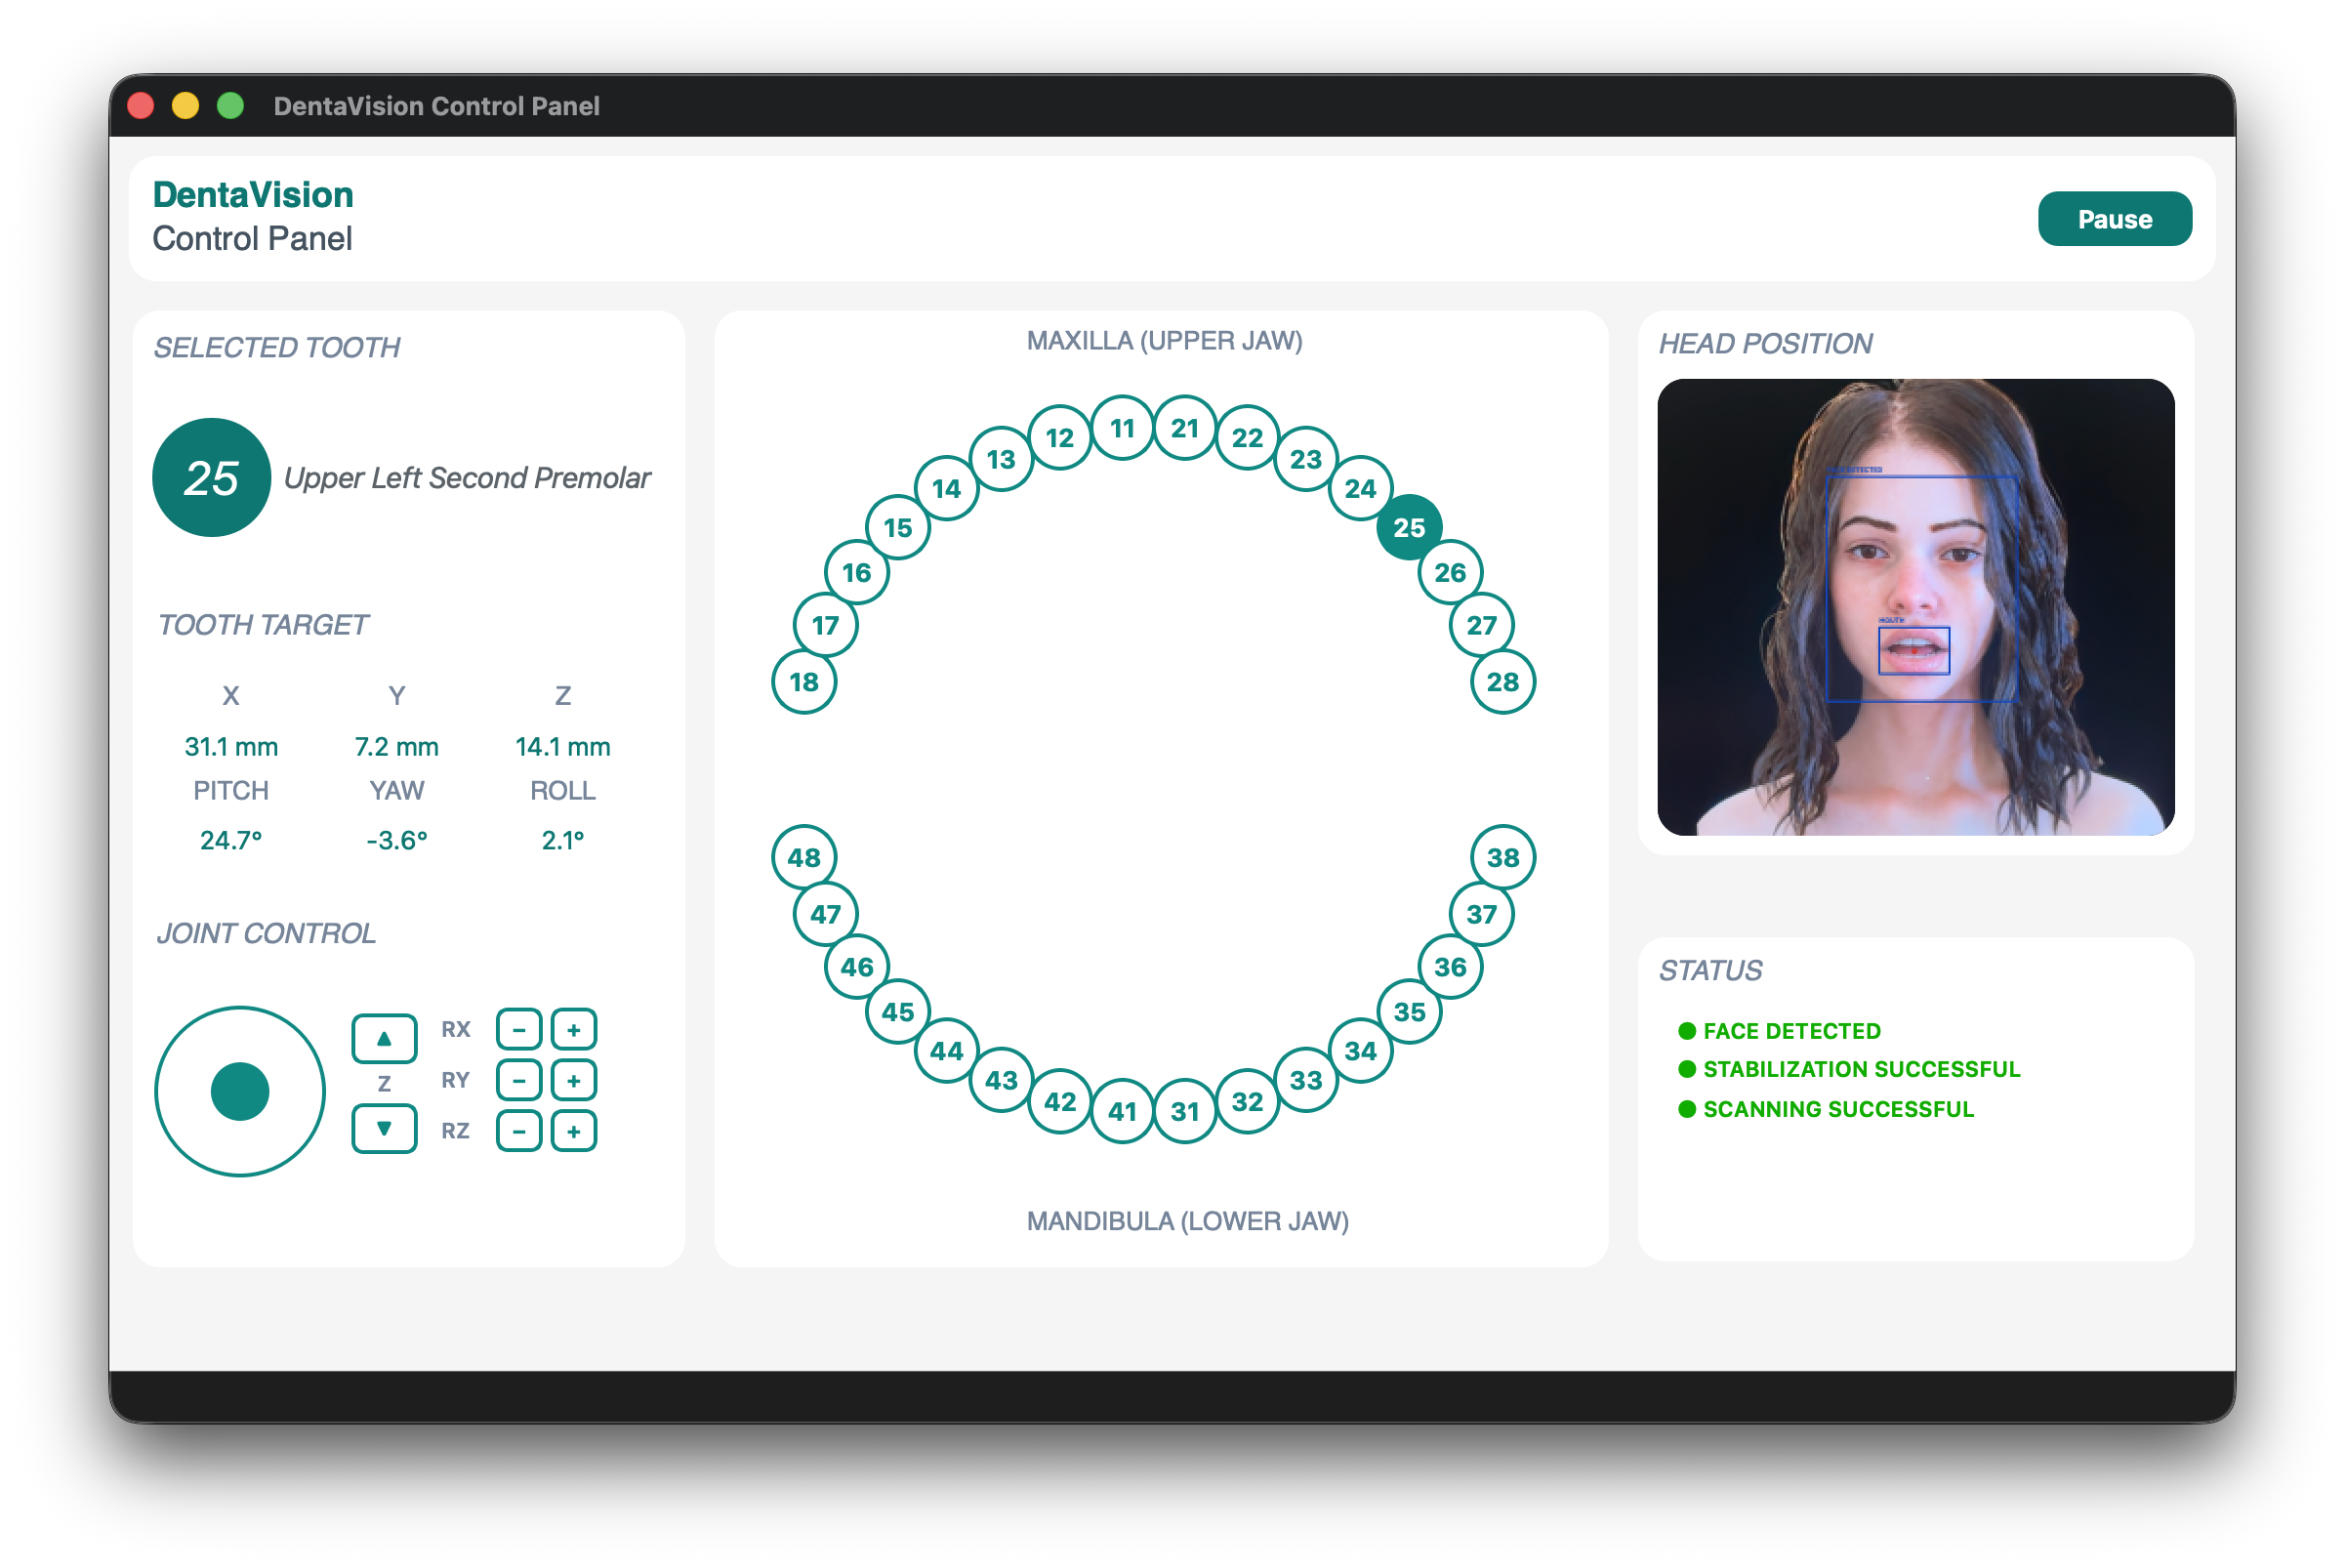
\includegraphics[width=\columnwidth,height=0.45\textheight,keepaspectratio]{ui_assets/demo4.png}
    \caption{Demo}
    \label{fig:demo_third}
\end{figure}

\begin{figure}[t]
    \centering
    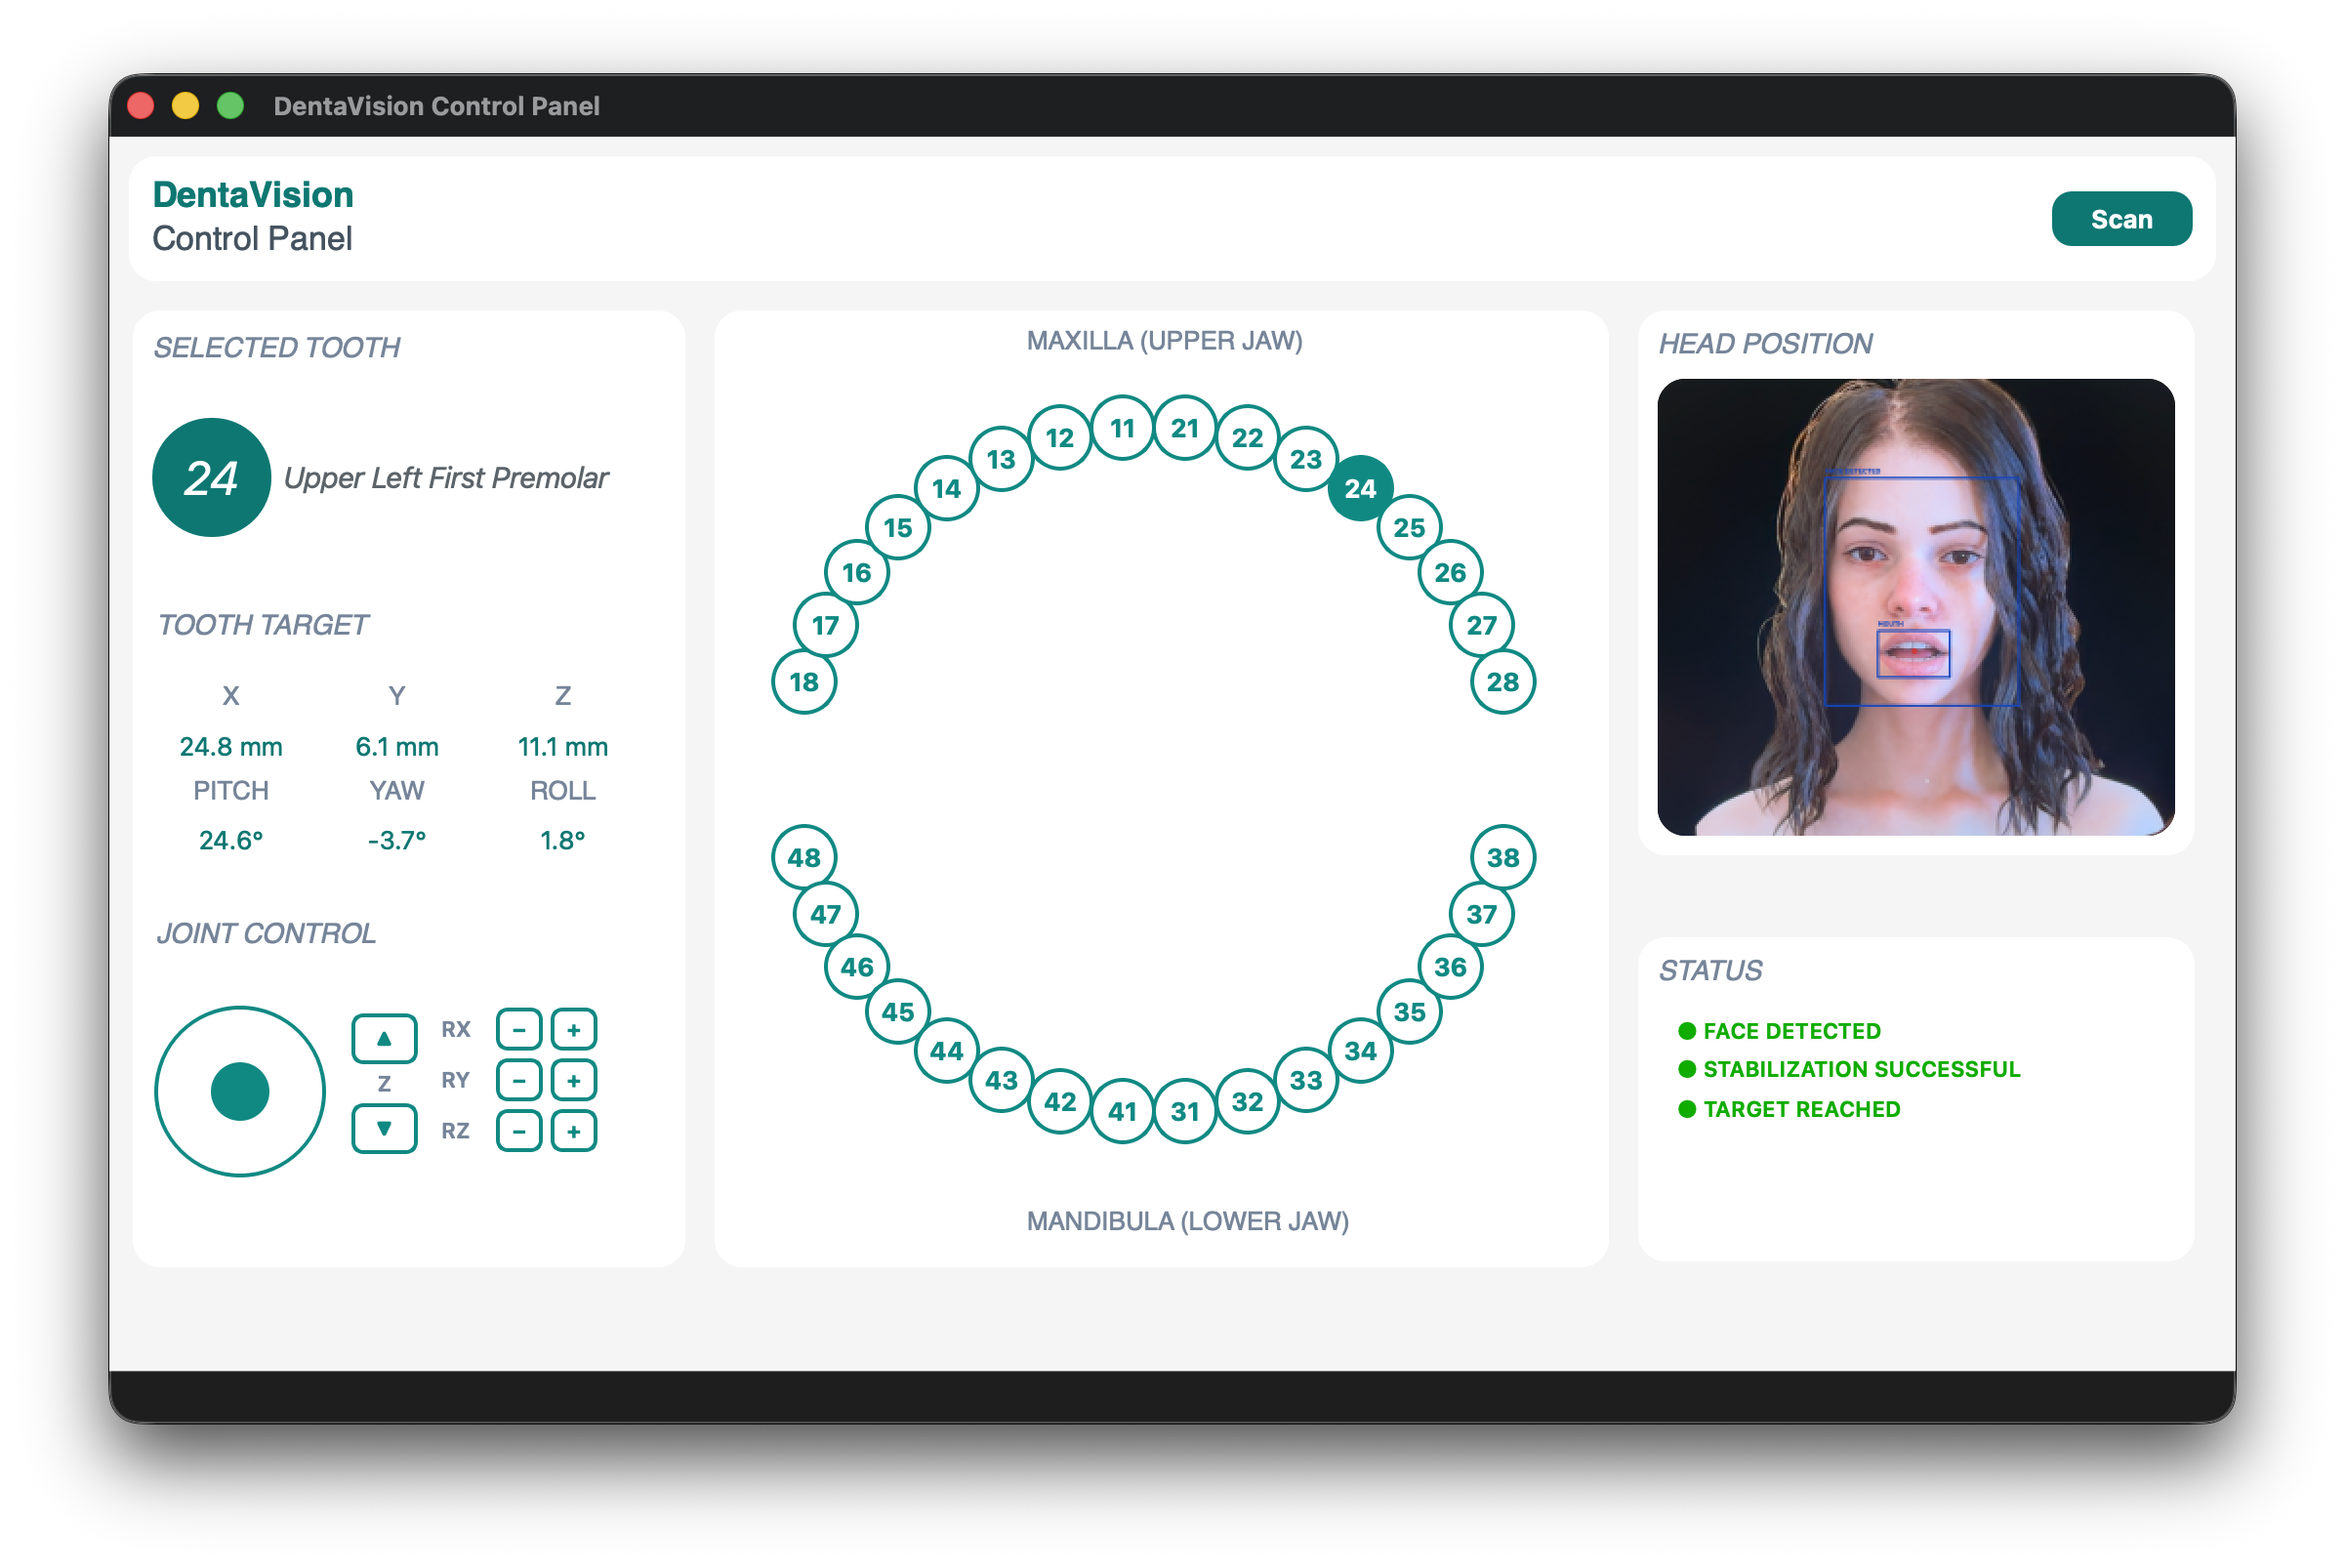
\includegraphics[width=\columnwidth,height=0.45\textheight,keepaspectratio]{ui_assets/demo4_6.png}
    \caption{Demo}
    \label{fig:demo_fourth}
\end{figure}

\section{Future Implementations}


\chapterbreak

\section{Conclusion}
\input{subpapers/05_conclusion}

\listoffigures

\printbibliography

\end{document}
